\documentclass[
%a5paper,
paper=5.5in:8.5in,
BCOR=7mm,
twoside,
DIV=calc,
11pt,
usegeometry,
chapterprefix,
headings=big]{scrbook} % Document font size and paper size

\usepackage{graphicx}
\usepackage{verse}
\usepackage{xcolor}
\usepackage{fontspec}
\usepackage[T1]{fontenc} % International character encodings
\usepackage{makeidx}
\usepackage{lettrine}
\usepackage{scrlayer-scrpage}
\usepackage{pifont}
\usepackage{enumitem}
\usepackage{caption}
\usepackage[maxlevel=3]{csquotes}
\usepackage[export]{adjustbox}
\usepackage{polyglossia}
\usepackage{afterpage}
\usepackage{microtype}
\usepackage{tocbasic}
\usepackage[pass]{geometry}
\usepackage{setspace}
\usepackage{subfiles}
\usepackage{rotating}
\usepackage[all]{nowidow}
\usepackage{setspaceenhanced}
\usepackage{ebgaramond} 
\usepackage{epigraph}
\usepackage{ellipsis}

\MakeAutoQuote{»}{«}
\catcode`\—=13
\protected\def—{\allowbreak\textemdash\allowbreak}
\newcommand\longdash{\mbox{---\,}\ignorespaces{}}

\setmainfont{EB Garamond}
\setdefaultlanguage[variant=uk]{english}
\setotherlanguage{french}
\newcommand{\HUGE}{\fontsize{35}{40}\selectfont}
\newcommand{\moderatelyhuge}{\fontsize{35}{45}\selectfont}
\newcommand{\reasonablyhuge}{\fontsize{30}{40}\selectfont}
\newfontfamily\chapterfont{EB Garamond}
%\newfontfamily\mytitlefont{GramophoneShadedNF.ttf}
%\newfontfamily\myauthorfont{Gramophone.NF.ttf}
\newfontfamily\mytitlefont{RaconteurNf-LOlE.ttf}
\newfontfamily\myauthorfont{RaconteurNf-LOlE.ttf}

\newfontfamily\lettrinefont{Decocaps.ttf}
\renewcommand{\LettrineFontHook}{\fontspec{Decocaps.ttf}}

\setkomafont{chapter}{\chapterfont\Huge\bfseries}
\addtokomafont{disposition}{\normalfont}
%\setkomafont{part}{\chapterfont\HUGE\bfseries}
%\addtokomafont{partnumber}{\chapterfont\moderatelyhuge}
%\renewcommand*{\partformat}{\partname~\thepart} %renew so it doesn't have the trailing period
\renewcommand*{\chapterformat}{\chaptername~\thechapter}
%\newcommand*\hideentrynumber[1]{}

\makeatletter
\@ifclasswith{scrbook}{a5paper}
{%
  \def\coverimagesize{0.7\linewidth}
%  \newcommand{\HUGE}{\fontsize{50}{60}\selectfont}
}{%
    \def\coverimagesize{0.8\linewidth}
%  \newcommand{\HUGE}{\fontsize{60}{70}\selectfont}
}
\makeatother

\newcount\zzc
\makeatletter
\def\zz{%
\ifnum\prevgraf<\c@L@lines
\zzc\z@
\loop
\ifnum\zzc<\prevgraf
\advance\zzc\@ne
\afterassignment\zzda\count@\L@parshape\relax
\repeat
\parshape\L@parshape
\fi}
\def\zzda{\afterassignment\zzdb\dimen@}
\def\zzdb{\afterassignment\zzdef\dimen@}
\def\zzdef#1\relax{\edef\L@parshape{\the\numexpr\count@-1\relax\space #1}}
\makeatother

\BeforeTOCHead[toc]{%
  \KOMAoptions{parskip=false}% no parskip in ToC
  \RedeclareSectionCommand[afterskip=1sp minus 1sp]{chapter}% no skip after ToC title
\DeclareTOCStyleEntry[beforeskip=0.1cm,entryformat=\chapterfont,linefill=\TOCLineLeaderFill]{chapter}{chapter}
}

\headsep=10pt
\headheight=45pt
\footskip=30pt

\defaultfontfeatures{Ligatures=TeX}

\automark{chapter}
\lehead{The Unpleasantness at the Bellona Club}
\rohead{\leftmark}
\flushbottom

\graphicspath{ {./images/} }


\hyphenation{}


\begin{document}
%\setlength{\epigraphwidth}{0.8\textwidth}
%\renewcommand{\epigraphflush}{center}
%\renewcommand{\sourceflush}{center}
%\renewcommand*{\chaptermarkformat}{}
%\renewcommand*{\chapterheadendvskip}{\vspace{10pt}}
%\renewcommand*{\chapterheadstartvskip}{\vspace{0pt}}

\frontmatter
\pagestyle{empty}
\begin{titlepage}

   \recalctypearea
 \newgeometry{left=10mm,right=10mm,top=7mm, bottom=7mm}

  \begin{center}\setstretch{1.8}\mytitlefont
  
{\setstretch{1.8}\reasonablyhuge The}\\
\vspace{0.4cm}
{\setstretch{1.8}\HUGE Unpleasantness}\\
\vspace{0.4cm}
{\setstretch{1.8}\reasonablyhuge at the}\\
\vspace{0.4cm}
{\HUGE Bellona Club}\\
\vfill
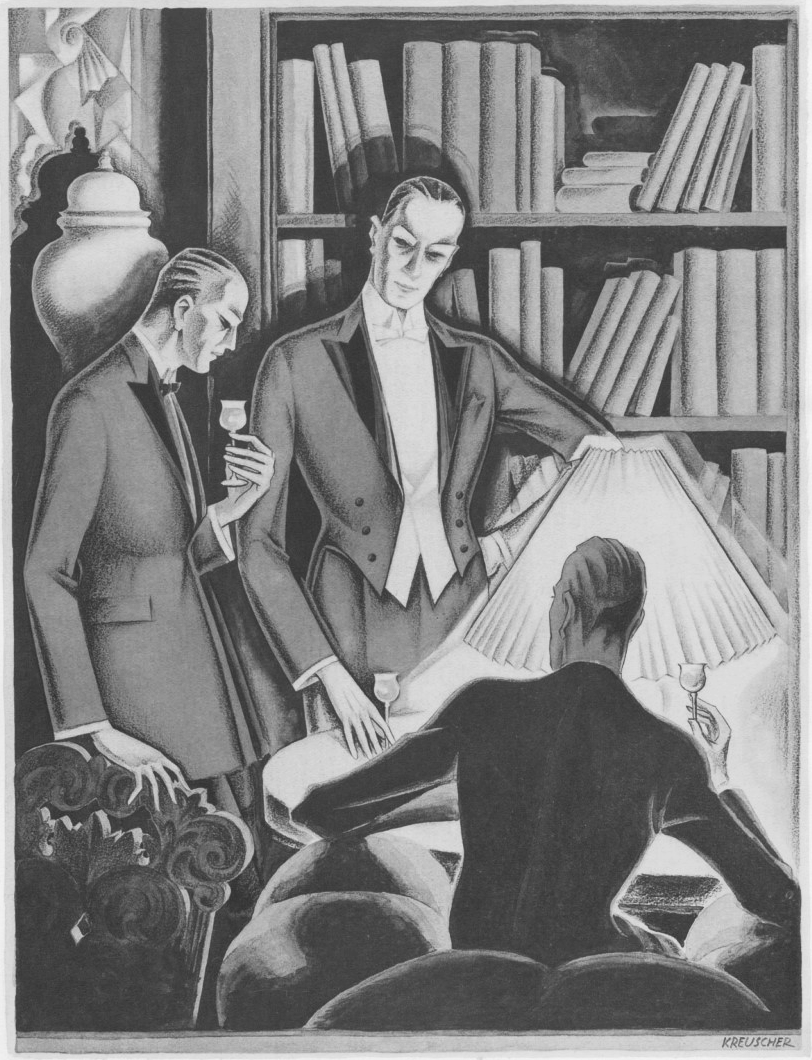
\includegraphics[width=\coverimagesize]{clubguys}\\
\vfill
\setstretch{1.5}\myauthorfont
{\setstretch{1.5}\reasonablyhuge Dorothy L. Sayers}\\
\end{center}
\recalctypearea
\restoregeometry
\end{titlepage}




\pagestyle{plain}

\renewcommand*\raggedchapter{\centering}



\KOMAoptions{headings=openleft}


%\vspace*{-2\baselineskip}
\tableofcontents
\enlargethispage{1.5\baselineskip}
\clearpage


%\clearpage






\mainmatter
\pagestyle{headings}
\renewcommand*{\chapterpagestyle}{plain}

\KOMAoptions{headings=openright}
%!TeX root=../bodytop.tex
\chapter[Chapter \thechapter]{}
\lettrine[lines=4,ante=‘]{O}{h}, damn!' said Lord Peter Wimsey at Piccadilly Circus. \enquote{Hi, driver!}

\zz
The taxi man, irritated at receiving this appeal while negotiating the intricacies of turning into Lower Regent Street across the route of a 19 ’bus, a 38-B and a bicycle, bent an unwilling ear.

\enquote{I’ve left the catalogue behind,} said Lord Peter deprecatingly. \enquote{Uncommonly careless of me. D’you mind puttin’ back to where we came from?}

\enquote{To the Savile Club, sir?}

\enquote{No\allowbreak---\allowbreak 110 Piccadilly\allowbreak---\allowbreak just beyond\allowbreak---\allowbreak thank you.}

\enquote{Thought you was in a hurry,} said the man, overcome with a sense of injury.

\enquote{I’m afraid it’s an awkward place to turn in,} said Lord Peter, answering the thought rather than the words. His long, amiable face looked as if it had generated spontaneously from his top hat, as white maggots breed from Gorgonzola.

The taxi, under the severe eye of a policeman, revolved by slow jerks, with a noise like the grinding of teeth.

The block of new, perfect and expensive flats in which Lord Peter dwelt upon the second floor, stood directly opposite the Green Park, in a spot for many years occupied by the skeleton of a frustrate commercial enterprise. As Lord Peter let himself in he heard his man’s voice in the library, uplifted in that throttled stridency peculiar to well-trained persons using the telephone.

\enquote{I believe that’s his lordship just coming in again\allowbreak---\allowbreak if your Grace would kindly hold the line a moment.}

\enquote{What is it, Bunter?}

\enquote{Her Grace has just called up from Denver, my lord. I was just saying your lordship had gone to the sale when I heard your lordship’s latchkey.}

\enquote{Thanks,} said Lord Peter; \enquote{and you might find me my catalogue, would you? I think I must have left it in my bedroom, or on the desk.}

He sat down to the telephone with an air of leisurely courtesy, as though it were an acquaintance dropped in for a chat.

\enquote{Hullo, Mother\allowbreak---\allowbreak that you?}

\enquote{Oh, there you are, dear,} replied the voice of the Dowager Duchess. \enquote{I was afraid I’d just missed you.}

\enquote{Well, you had, as a matter of fact. I’d just started off to Brocklebury’s sale to pick up a book or two, but I had to come back for the catalogue. What’s up?}

\enquote{Such a quaint thing,} said the Duchess. \enquote{I thought I’d tell you. You know little Mr Thipps?}

\enquote{Thipps?} said Lord Peter. \enquote{Thipps? Oh, yes, the little architect man who’s doing the church roof. Yes. What about him?}

\enquote{Mrs Throgmorton’s just been in, in quite a state of mind.}

\enquote{Sorry, Mother, I can’t hear. Mrs Who?}

\enquote{Throgmorton\allowbreak---\allowbreak Throgmorton---the vicar’s wife.}

\enquote{Oh, Throgmorton, yes?}

\enquote{Mr Thipps rang them up this morning. It was his day to come down, you know.}

\enquote{Yes?}

\enquote{He rang them up to say he couldn’t. He was so upset, poor little man. He’d found a dead body in his bath.}

\enquote{Sorry, Mother, I can’t hear; found what, where?}

\enquote{A dead body, dear, in his bath.}

\enquote{What?---no, no, we haven’t finished. Please don’t cut us off. Hullo! Hullo! Is that you, Mother? Hullo!---Mother!---Oh, yes\allowbreak---\allowbreak sorry, the girl was trying to cut us off. What sort of body?}

\enquote{A dead man, dear, with nothing on but a pair of pince-nez. Mrs Throgmorton positively blushed when she was telling me. I’m afraid people do get a little narrow-minded in country vicarages.}

\enquote{Well, it sounds a bit unusual. Was it anybody he knew?}

\enquote{No, dear, I don’t think so, but, of course, he couldn’t give her many details. She said he sounded quite distracted. He’s such a respectable little man\allowbreak---\allowbreak and having the police in the house and so on, really worried him.}

\enquote{Poor little Thipps! Uncommonly awkward for him. Let’s see, he lives in Battersea, doesn’t he?}

\enquote{Yes, dear; 59, Queen Caroline Mansions; opposite the Park. That big block just round the corner from the Hospital. I thought perhaps you’d like to run round and see him and ask if there’s anything we can do. I always thought him a nice little man.}

\enquote{Oh, quite,} said Lord Peter, grinning at the telephone. The Duchess was always of the greatest assistance to his hobby of criminal investigation, though she never alluded to it, and maintained a polite fiction of its non-existence.

\enquote{What time did it happen, Mother?}

\enquote{I think he found it early this morning, but, of course, he didn’t think of telling the Throgmortons just at first. She came up to me just before lunch\allowbreak---\allowbreak so tiresome, I had to ask her to stay. Fortunately, I was alone. I don’t mind being bored myself, but I hate having my guests bored.}

\enquote{Poor old Mother! Well, thanks awfully for tellin’ me. I think I’ll send Bunter to the sale and toddle round to Battersea now an’ try and console the poor little beast. So-long.}

\enquote{Good-bye, dear.}

\enquote{Bunter!}

\enquote{Yes, my lord.}

\enquote{Her Grace tells me that a respectable Battersea architect has discovered a dead man in his bath.}

\enquote{Indeed, my lord? That’s very gratifying.}

\enquote{Very, Bunter. Your choice of words is unerring. I wish Eton and Balliol had done as much for me. Have you found the catalogue?}

\enquote{Here it is, my lord.}

\enquote{Thanks. I am going to Battersea at once. I want you to attend the sale for me. Don’t lose time\allowbreak---\allowbreak I don’t want to miss the Folio Dante\footnote{This is the first Florence edition, 1481, by Niccolo di Lorenzo. Lord Peter’s collection of printed Dantes is worth inspection. It includes, besides the famous Aldine 8vo. of 1502, the Naples folio of 1477—\enquote{edizione rarissima,} according to Colomb. This copy has no history, and Mr. Parker’s private belief is that its present owner conveyed it away by stealth from somewhere or other. Lord Peter’s own account is that he \enquote{picked it up in a little place in the hills,} when making a walking-tour through Italy.} nor the de Voragine\allowbreak---\allowbreak here you are\allowbreak---\allowbreak see? \textit{Golden Legend}---Wynkyn de Worde, 1493\allowbreak---\allowbreak got that?---and, I say, make a special effort for the Caxton folio of the \textit{Four Sons of Aymon}---it’s the 1489 folio and unique. Look! I’ve marked the lots I want, and put my outside offer against each. Do your best for me. I shall be back to dinner.}

\enquote{Very good, my lord.}

\enquote{Take my cab and tell him to hurry. He may for you; he doesn’t like me very much. Can I,} said Lord Peter, looking at himself in the eighteenth-century mirror over the mantelpiece, \enquote{can I have the heart to fluster the flustered Thipps further\allowbreak---\allowbreak that’s very difficult to say quickly\allowbreak---\allowbreak by appearing in a top-hat and frock-coat? I think not. Ten to one he will overlook my trousers and mistake me for the undertaker. A grey suit, I fancy, neat but not gaudy, with a hat to tone, suits my other self better. Exit the amateur of first editions; new motive introduced by solo bassoon; enter Sherlock Holmes, disguised as a walking gentleman. There goes Bunter. Invaluable fellow\allowbreak---\allowbreak never offers to do his job when you’ve told him to do somethin’ else. Hope he doesn’t miss the \textit{Four Sons of Aymon}. Still, there \textit{is} another copy of that\allowbreak---\allowbreak in the Vatican.\footnote{Lord Peter’s wits were wool-gathering. The book is in the possession of Earl Spencer. The Brocklebury copy is incomplete, the last five signatures being altogether missing, but is unique in possessing the colophon.} It might become available, you never know\allowbreak---\allowbreak if the Church of Rome went to pot or Switzerland invaded Italy\allowbreak---\allowbreak whereas a strange corpse doesn’t turn up in a suburban bathroom more than once in a lifetime\allowbreak---\allowbreak at least, I should think not\allowbreak---\allowbreak at any rate, the number of times it’s happened, \textit{with} a pince-nez, might be counted on the fingers of one hand, I imagine. Dear me! it’s a dreadful mistake to ride two hobbies at once.}

He had drifted across the passage into his bedroom, and was changing with a rapidity one might not have expected from a man of his mannerisms. He selected a dark-green tie to match his socks and tied it accurately without hesitation or the slightest compression of his lips; substituted a pair of brown shoes for his black ones, slipped a monocle into a breast pocket, and took up a beautiful Malacca walking-stick with a heavy silver knob.

\enquote{That’s all, I think,} he murmured to himself. \enquote{Stay\allowbreak---\allowbreak I may as well have you\allowbreak---\allowbreak you may come in useful\allowbreak---\allowbreak one never knows.} He added a flat silver matchbox to his equipment, glanced at his watch, and seeing that it was already a quarter to three, ran briskly downstairs, and, hailing a taxi, was carried to Battersea Park.

Mr Alfred Thipps was a small, nervous man, whose flaxen hair was beginning to abandon the unequal struggle with destiny. One might say that his only really marked feature was a large bruise over the left eyebrow, which gave him a faintly dissipated air incongruous with the rest of his appearance. Almost in the same breath with his first greeting, he made a self-conscious apology for it, murmuring something about having run against the dining-room door in the dark. He was touched almost to tears by Lord Peter’s thoughtfulness and condescension in calling.

\enquote{I’m sure it’s most kind of your lordship,} he repeated for the dozenth time, rapidly blinking his weak little eyelids. \enquote{I appreciate it very deeply, very deeply, indeed, and so would Mother, only she’s so deaf, I don’t like to trouble you with making her understand. It’s been very hard all day,} he added, \enquote{with the policemen in the house and all this commotion. It’s what Mother and me have never been used to, always living very retired, and it’s most distressing to a man of regular habits, my lord, and reely, I’m almost thankful Mother doesn’t understand, for I’m sure it would worry her terribly if she was to know about it. She was upset at first, but she’s made up some idea of her own about it now, and I’m sure it’s all for the best.}

The old lady who sat knitting by the fire nodded grimly in response to a look from her son.

\enquote{I always said as you ought to complain about that bath, Alfred,} she said suddenly, in the high, piping voice peculiar to the deaf, \enquote{and it’s to be ’oped the landlord’ll see about it now; not but what I think you might have managed without having the police in, but there! you always were one to make a fuss about a little thing, from chicken-pox up.}

\enquote{There now,} said Mr Thipps apologetically, \enquote{you see how it is. Not but what it’s just as well she’s settled on that, because she understands we’ve locked up the bathroom and don’t try to go in there. But it’s been a terrible shock to me, sir\allowbreak---\allowbreak my lord, I should say, but there! my nerves are all to pieces. Such a thing has never ’appened\allowbreak---\allowbreak happened to me in all my born days. Such a state I was in this morning\allowbreak---\allowbreak I didn’t know if I was on my head or my heels\allowbreak---\allowbreak I reely didn’t, and my heart not being too strong, I hardly knew how to get out of that horrid room and telephone for the police. It’s affected me, sir, it’s affected me, it reely has\allowbreak---\allowbreak I couldn’t touch a bit of breakfast, nor lunch neither, and what with telephoning and putting off clients and interviewing people all morning, I’ve hardly known what to do with myself.}

\enquote{I’m sure it must have been uncommonly distressin’,} said Lord Peter, sympathetically, \enquote{especially comin’ like that before breakfast. Hate anything tiresome happenin’ before breakfast. Takes a man at such a confounded disadvantage, what?}

\enquote{That’s just it, that’s just it,} said Mr Thipps, eagerly. \enquote{When I saw that dreadful thing lying there in my bath, mother-naked, too, except for a pair of eyeglasses, I assure you, my lord, it regularly turned my stomach, if you’ll excuse the expression. I’m not very strong, sir, and I get that sinking feeling sometimes in the morning, and what with one thing and another I ’ad\allowbreak---\allowbreak had to send the girl for a stiff brandy, or I don’t know \textit{what} mightn’t have happened. I felt so queer, though I’m anything but partial to spirits as a rule. Still, I make it a rule never to be without brandy in the house, in case of emergency, you know?}

\enquote{Very wise of you,} said Lord Peter, cheerfully. \enquote{You’re a very far-seein’ man, Mr Thipps. Wonderful what a little nip’ll do in case of need, and the less you’re used to it the more good it does you. Hope your girl is a sensible young woman, what? Nuisance to have women faintin’ and shriekin’ all over the place.}

\enquote{Oh, Gladys is a good girl,} said Mr Thipps, \enquote{very reasonable indeed. She was shocked, of course; that’s very understandable. I was shocked myself, and it wouldn’t be proper in a young woman not to be shocked under the circumstances, but she is reely a helpful, energetic girl in a crisis, if you understand me. I consider myself very fortunate these days to have got a good, decent girl to do for me and Mother, even though she is a bit careless and forgetful about little things, but that’s only natural. She was very sorry indeed about having left the bathroom window open, she reely was, and though I was angry at first, seeing what’s come of it, it wasn’t anything to speak of, not in the ordinary way, as you might say. Girls will forget things, you know, my lord, and reely she was so distressed I didn’t like to say too much to her. All I said was: \enquote{It might have been burglars,} I said, \enquote{remember that, next time you leave a window open all night; this time it was a dead man,} I said, \enquote{and that’s unpleasant enough, but next time it might be burglars,} I said, \enquote{and all of us murdered in our beds.} But the police-inspector\allowbreak---\allowbreak Inspector Sugg, they called him, from the Yard\allowbreak---\allowbreak he was very sharp with her, poor girl. Quite frightened her, and made her think he suspected her of something, though what good a body could be to her, poor girl, I can’t imagine, and so I told the Inspector. He was quite rude to me, my lord\allowbreak---\allowbreak I may say I didn’t like his manner at all. \enquote{If you’ve got anything definite to accuse Gladys or me of, Inspector,} I said to him, \enquote{bring it forward, that’s what you have to do,} I said, \enquote{but I’ve yet to learn that you’re paid to be rude to a gentleman in his own ’ouse\allowbreak---\allowbreak house.} Reely,} said Mr Thipps, growing quite pink on the top of his head, \enquote{he regularly roused me, regularly roused me, my lord, and I’m a mild man as a rule.}

\enquote{Sugg all over,} said Lord Peter. \enquote{I know him. When he don’t know what else to say, he’s rude. Stands to reason you and the girl wouldn’t go collectin’ bodies. Who’d want to saddle himself with a body? Difficulty’s usually to get rid of ’em. Have you got rid of this one yet, by the way?}

\enquote{It’s still in the bathroom,} said Mr Thipps. \enquote{Inspector Sugg said nothing was to be touched till his men came in to move it. I’m expecting them at any time. If it would interest your lordship to have a look at it\longdash}

\enquote{Thanks awfully,} said Lord Peter. \enquote{I’d like to very much, if I’m not puttin’ you out.}

\enquote{Not at all,} said Mr Thipps. His manner as he led the way along the passage convinced Lord Peter of two things\allowbreak---\allowbreak first, that, gruesome as his exhibit was, he rejoiced in the importance it reflected upon himself and his flat, and secondly, that Inspector Sugg had forbidden him to exhibit it to anyone. The latter supposition was confirmed by the action of Mr Thipps, who stopped to fetch the door-key from his bedroom, saying that the police had the other, but that he made it a rule to have two keys to every door, in case of accident.

The bathroom was in no way remarkable. It was long and narrow, the window being exactly over the head of the bath. The panes were of frosted glass; the frame wide enough to admit a man’s body. Lord Peter stepped rapidly across to it, opened it and looked out.

The flat was the top one of the building and situated about the middle of the block. The bathroom window looked out upon the back-yards of the flats, which were occupied by various small outbuildings, coal-holes, garages, and the like. Beyond these were the back gardens of a parallel line of houses. On the right rose the extensive edifice of St Luke’s Hospital, Battersea, with its grounds, and, connected with it by a covered way, the residence of the famous surgeon, Sir Julian Freke, who directed the surgical side of the great new hospital, and was, in addition, known in Harley Street as a distinguished neurologist with a highly individual point of view.

This information was poured into Lord Peter’s ear at considerable length by Mr Thipps, who seemed to feel that the neighbourhood of anybody so distinguished shed a kind of halo of glory over Queen Caroline Mansions.

\enquote{We had him round here himself this morning,} he said, \enquote{about this horrid business. Inspector Sugg thought one of the young medical gentlemen at the hospital might have brought the corpse round for a joke, as you might say, they always having bodies in the dissecting-room. So Inspector Sugg went round to see Sir Julian this morning to ask if there was a body missing. He was very kind, was Sir Julian, very kind indeed, though he was at work when they got there, in the dissecting-room. He looked up the books to see that all the bodies were accounted for, and then very obligingly came round here to look at this}---he indicated the bath---\enquote{and said he was afraid he couldn’t help us\allowbreak---\allowbreak there was no corpse missing from the hospital, and this one didn’t answer to the description of any they’d had.}

\enquote{Nor to the description of any of the patients, I hope,} suggested Lord Peter casually.

At this grisly hint Mr Thipps turned pale.

\enquote{I didn’t hear Inspector Sugg inquire,} he said, with some agitation. \enquote{What a very horrid thing that would be\allowbreak---\allowbreak God bless my soul, my lord, I never thought of it.}

\enquote{Well, if they had missed a patient they’d probably have discovered it by now,} said Lord Peter. \enquote{Let’s have a look at this one.}

He screwed his monocle into his eye, adding: \enquote{I see you’re troubled here with the soot blowing in. Beastly nuisance, ain’t it? I get it, too\allowbreak---\allowbreak spoils all my books, you know. Here, don’t you trouble, if you don’t care about lookin’ at it.}

He took from Mr Thipps’s hesitating hand the sheet which had been flung over the bath, and turned it back.

The body which lay in the bath was that of a tall, stout man of about fifty. The hair, which was thick and black and naturally curly, had been cut and parted by a master hand, and exuded a faint violet perfume, perfectly recognisable in the close air of the bathroom. The features were thick, fleshy and strongly marked, with prominent dark eyes, and a long nose curving down to a heavy chin. The clean-shaven lips were full and sensual, and the dropped jaw showed teeth stained with tobacco. On the dead face the handsome pair of gold pince-nez mocked death with grotesque elegance; the fine gold chain curved over the naked breast. The legs lay stiffly stretched out side by side; the arms reposed close to the body; the fingers were flexed naturally. Lord Peter lifted one arm, and looked at the hand with a little frown.

\enquote{Bit of a dandy, your visitor, what?} he murmured. \enquote{Parma violet and manicure.} He bent again, slipping his hand beneath the head. The absurd eyeglasses slipped off, clattering into the bath, and the noise put the last touch to Mr Thipps’s growing nervousness.

\enquote{If you’ll excuse me,} he murmured, \enquote{it makes me feel quite faint, it reely does.}

He slipped outside, and he had no sooner done so than Lord Peter, lifting the body quickly and cautiously, turned it over and inspected it with his head on one side, bringing his monocle into play with the air of the late Joseph Chamberlain approving a rare orchid. He then laid the head over his arm, and bringing out the silver matchbox from his pocket, slipped it into the open mouth. Then making the noise usually written \enquote{Tut-tut,} he laid the body down, picked up the mysterious pince-nez, looked at it, put it on his nose and looked through it, made the same noise again, readjusted the pince-nez upon the nose of the corpse, so as to leave no traces of interference for the irritation of Inspector Sugg; rearranged the body; returned to the window and, leaning out, reached upwards and sideways with his walking-stick, which he had somewhat incongruously brought along with him. Nothing appearing to come of these investigations, he withdrew his head, closed the window, and rejoined Mr Thipps in the passage.

Mr Thipps, touched by this sympathetic interest in the younger son of a duke, took the liberty, on their return to the sitting-room, of offering him a cup of tea. Lord Peter, who had strolled over to the window and was admiring the outlook on Battersea Park, was about to accept, when an ambulance came into view at the end of Prince of Wales Road. Its appearance reminded Lord Peter of an important engagement, and with a hurried \enquote{By Jove!} he took his leave of Mr Thipps.

\enquote{My mother sent kind regards and all that,} he said, shaking hands fervently; \enquote{hopes you’ll soon be down at Denver again. Good-bye, Mrs Thipps,} he bawled kindly into the ear of the old lady. \enquote{Oh, no, my dear sir, please don’t trouble to come down.}

He was none too soon. As he stepped out of the door and turned towards the station, the ambulance drew up from the other direction, and Inspector Sugg emerged from it with two constables. The Inspector spoke to the officer on duty at the Mansions, and turned a suspicious gaze on Lord Peter’s retreating back.

\enquote{Dear old Sugg,} said that nobleman, fondly, \enquote{dear, dear old bird! How he does hate me, to be sure.}
%!TeX root=../cloudstop.tex


\chapter{The Green-Eyed Cat}

\epigraph{And here's to the hound\\With his nose unto the ground}{»Drink, Puppy, Drink«}


\lettrine[lines=4]{S}{ome} people hold that breakfast is the best meal of the day. Others, less robust, hold that it is the worst, and that, of all breakfasts in the week, Sunday morning breakfast is incomparably the worst.

\zz
The party gathered about the breakfast-table at Riddlesdale Lodge held, if one might judge from their faces, no brief for that day miscalled of sweet refection and holy love. The only member of it who seemed neither angry nor embarrassed was the Hon. Freddy Arbuthnot, and he was silent, engaged in trying to take the whole skeleton out of a bloater at once.  The very presence of that undistinguished fish upon the Duchess's breakfast-table indicated a disorganized household.

The Duchess of Denver was pouring out coffee. This was one of her uncomfortable habits. Persons arriving late for breakfast were thereby made painfully aware of their sloth. She was a long-necked, long-backed woman, who disciplined her hair and her children. She was never embarrassed, and her anger, though never permitted to be visible, made itself felt the more.

Colonel and Mrs~Marchbanks sat side by side. They had nothing beautiful about them but a stolid mutual affection. Mrs~Marchbanks was not angry, but she was embarrassed in the presence of the Duchess, because she could not feel sorry for her. When you felt sorry for people you called them »poor old dear« or »poor dear old man.« Since, obviously, you could not call the Duchess poor old dear, you were not being properly sorry for her. This distressed Mrs~Marchbanks. The Colonel was both embarrassed and angry—embarrassed because, 'pon my soul, it was very difficult to know what to talk about in a house where your host had been arrested for murder; angry in a dim way, like an injured animal, because unpleasant things like this had no business to break in on the shooting-season.

Mrs~Pettigrew-Robinson was not only angry, she was outraged. As a girl she had adopted the motto stamped upon the school notepaper: \textit{Quœcunque honesta}. She had always thought it \textit{wrong} to let your mind \textit{dwell} on anything that was not really nice. In middle life she still made a point of ignoring those newspaper paragraphs which bore such headlines as: »\textsc{Assault upon a School teacher at Cricklewood}«; »\textsc{Death in a Pint of Stout}«; »\textsc{\textsterling 75 for a Kiss}«; or »\textsc{She called him Hubbykins}«. She said she could not see what \textit{good} it did you to know about such things. She regretted having consented to visit Riddlesdale Lodge in the absence of the Duchess. She had never liked Lady~Mary; she considered her a very objectionable specimen of the modern independent young woman; besides, there had been that very undignified incident connected with a Bolshevist while Lady~Mary was nursing in London during the war. Nor had Mrs~Pettigrew-Robinson at all cared for Captain Denis Cathcart. She did not like a young man to be handsome in that obvious kind of way. But, of course, since Mr~Pettigrew-Robinson had wanted to come to Riddlesdale, it was her place to be with him. She was not to blame for the unfortunate result.

Mr~Pettigrew-Robinson was angry, quite simply, because the detective from Scotland Yard had not accepted his help in searching the house and grounds for footprints. As an older man of some experience in these matters (Mr~Pettigrew-Robinson was a county magistrate) he had gone out of his way to place himself at the man's disposal. Not only had the man been short with him, but he had rudely ordered him out of the conservatory, where he (Mr~Pettigrew-Robinson) had been reconstructing the affair from the point of view of Lady~Mary.

All these angers and embarrassments might have caused less pain to the company had they not been aggravated by the presence of the detective himself, a quiet young man in a tweed suit, eating curry at one end of the table next to Mr~Murbles, the solicitor. This person had arrived from London on Friday, had corrected the local police, and strongly dissented from the opinion of Inspector~Craikes. He had suppressed at the inquest information which, if openly given, might have precluded the arrest of the Duke. He had officiously detained the whole unhappy party, on the grounds that he wanted to re-examine everybody, and was thus keeping them miserably cooped up together over a horrible Sunday; and he had put the coping-stone on his offences by turning out to be an intimate friend of Lord~Peter Wimsey's, and having, in consequence, to be accommodated with a bed in the gamekeeper's cottage and breakfast at the Lodge.

Mr~Murbles, who was elderly and had a delicate digestion, had travelled up in a hurry on Thursday night. He had found the inquest very improperly conducted and his client altogether impracticable. He had spent all his time trying to get hold of Sir Impey Biggs, \textsc{k.c.}, who had vanished for the weekend, leaving no address. He was eating a little dry toast, and was inclined to like the detective, who called him »Sir«, and passed him the butter.

»Is anybody thinking of going to church?« asked the Duchess.

»Theodore and I should like to go,« said Mrs~Pettigrew-Robinson, »if it is not too much trouble; or we could walk. It is not so \textit{very} far.«

»It's two and a half miles, good,« said Colonel Marchbanks.

Mr~Pettigrew-Robinson looked at him gratefully.

»Of course you will come in the car,« said the Duchess. »I am going myself.«

»Are you, though?« said the Hon. Freddy. »I say, won't you get a bit stared at, what?«

»Really, Freddy,« said the Duchess, »does that matter?«

»Well,« said the Hon. Freddy, »I mean to say, these bounders about here are all Socialists and Methodists\dots«

»If they are Methodists,« said Mrs~Pettigrew-Robinson, »they will not be at church.«

»Won't they?« retorted the Hon. Freddy. »You bet they will if there's anything to see. Why, it'll be better'n a funeral to 'em.«

»Surely,« said Mrs~Pettigrew-Robinson, »one has a \textit{duty} in the matter, whatever our private feelings may be—especially at the present day, when people are so terribly \textit{slack}.«

She glanced at the Hon. Freddy.

»Oh, don't you mind me, Mrs~P\@.,« said that youth amiably. »All \textit{I} say is, if these blighters make things unpleasant, don't blame me.«

»Whoever thought of blaming you, Freddy?« said the Duchess.

»Manner of speaking,« said the Hon. Freddy.

»What do you think, Mr~Murbles?« inquired her ladyship.

»I feel,« said the lawyer, carefully stirring his coffee, »that, while your intention is a very admirable one, and does you very great credit, my dear lady, yet Mr~Arbuthnot is right in saying it may involve you in some—er—unpleasant publicity. Er—I have always been a sincere Christian myself, but I cannot feel that our religion demands that we should make ourselves conspicuous—er—in such very painful circumstances.«

Mr~Parker reminded himself of a dictum of Lord~Melbourne.

»Well, after all,« said Mrs~Marchbanks, »as Helen so rightly says, does it matter? Nobody's really got anything to be ashamed of. There has been a stupid mistake, of course, but I don't see why anybody who wants to shouldn't go to church.«

»Certainly not, certainly not, my dear,« said the Colonel heartily. »We might look in ourselves, eh, dear? Take a walk that way I mean, and come out before the sermon. I think it's a good thing. Shows \textit{we} don't believe old Denver's done anything wrong, anyhow.«

»You forget, dear,« said his wife, »I've promised to stay at home with Mary, poor girl.«

»Of course, of course—stupid of me,« said the Colonel. »How is she?«

»She was very restless last night, poor child,« said the Duchess.  »Perhaps she will get a little sleep this morning. It has been a shock to her.«

»One which may prove a blessing in disguise,« said Mrs~Pettigrew-Robinson.

»My dear!« said her husband.

»Wonder when we shall hear from Sir Impey,« said Colonel Marchbanks hurriedly.

»Yes, indeed,« moaned Mr~Murbles. »I am counting on his influence with the Duke.«

»Of course,« said Mrs~Pettigrew-Robinson, »he must speak out—for everybody's sake. He must say what he was doing out of doors at that time. Or, if he does not, it must be discovered. Dear me! That's what these detectives are for, aren't they?«

»That is their ungrateful task,« said Mr~Parker suddenly. He had said nothing for a long time, and everybody jumped.

»There,« said Mrs~Marchbanks, »I expect you'll clear it all up in no time, Mr~Parker. Perhaps you've got the real mur—the culprit up your sleeve all the time.«

»Not quite,« said Mr~Parker, »but I'll do my best to get him.  Besides,« he added, with a grin, »I'll probably have some help on the job.«

»From whom?« inquired Mr~Pettigrew-Robinson.

»Her grace's brother-in-law.«

»Peter?« said the Duchess. »Mr~Parker must be amused at the family amateur,« she added.

»Not at all,« said Parker. »Wimsey would be one of the finest detectives in England if he wasn't lazy. Only we can't get hold of him.«

»I've wired to Ajaccio—poste restante,« said Mr~Murbles, »but I don't know when he's likely to call there. He said nothing about when he was coming back to England.«

»He's a rummy old bird,« said the Hon. Freddy tactlessly, »but he oughter be here, what? What I mean to say is, if anything happens to old Denver, don't you see, he's the head of the family, ain't he—till little Pickled Gherkins comes of age.«

In the frightful silence which followed this remark, the sound of a walking-stick being clattered into an umbrella-stand was distinctly
audible.

»Who's that, I wonder,« said the Duchess.

The door waltzed open.

»Mornin', dear old things,« said the newcomer cheerfully. »How are you all? Hullo, Helen! Colonel, you owe me half a crown since last September year. Mornin', Mrs~Marchbanks, Mornin', Mrs~P\@. Well, Mr~Murbles, how d'you like this bili-beastly weather? Don't trouble to get up, Freddy; I'd simply hate to inconvenience you. Parker, old man, what a damned reliable old bird you are! Always on the spot, like that patent ointment thing. I say, have you all finished? I meant to get up earlier, but I was snorin' so Bunter hadn't the heart to wake me. I nearly blew in last night, only we didn't arrive till 2 \textsc{a.m.} and I thought you wouldn't half bless me if I did. Eh, what, Colonel? Airplane \textit{Victoria} from Paris to London—North-Eastern to Northallerton—damn bad roads the rest of the way, and a puncture just below Riddlesdale. Damn bad bed at the »Lord~in Glory«; thought I'd blow in for the last sausage here, if I was lucky. What? Sunday morning in an English family and no sausages? God bless my soul, what's the world coming to, eh, Colonel? I say, Helen, old Gerald's been an' gone an' done it this time, what? You've no business to leave him on his own, you know; he always gets into mischief. What's that? Curry? Thanks, old man. Here, I say, you needn't be so stingy about it; I've been travelling for three days on end. Freddy, pass the toast. Beg pardon, Mrs~Marchbanks? Oh, rather, yes; Corsica was perfectly amazin'—all black-eyed fellows with knives in their belts and jolly fine-looking girls. Old Bunter had a regular affair with the innkeeper's daughter in one place. D'you know, he's an awfully susceptible old beggar. You'd never think it, would you? Jove! I am hungry. I say, Helen, I meant to get you some fetchin' crêpe-de-Chine undies from Paris, but I saw that old Parker was gettin' ahead of me over the bloodstains, so we packed up our things and buzzed off.«

Mrs~Pettigrew-Robinson rose.

»Theodore,« she said, »I think we ought to be getting ready for church.«

»I will order the car,« said the Duchess. »Peter, of course I'm exceedingly glad to see you. Your leaving no address was most inconvenient. Ring for anything you want. It is a pity you didn't arrive in time to see Gerald.«

»Oh, that's all right,« said Lord~Peter cheerfully; »I'll look him up in quod. Y'know, it's rather a good idea to keep one's crimes in the family; one has so many more facilities. I'm sorry for poor old Polly, though. How is she?«

»She must not be disturbed today,« said the Duchess with decision.

»Not a bit of it,« said Lord~Peter; »she'll keep. Today Parker and I hold high revel. Today he shows me all the bloody footprints—it's all right, Helen, that's not swearin', that's an adjective of quality. I hope they aren't all washed away, are they, old thing?«

»No,« said Parker, »I've got most of them under flower-pots.«

»Then pass the bread and squish,« said Lord~Peter, »and tell me all about it.«

The departure of the church-going element had induced a more humanitarian atmosphere. Mrs~Marchbanks stumped off upstairs to tell Mary that Peter had come, and the Colonel lit a large cigar. The Hon.  Freddy rose, stretched himself, pulled a leather armchair to the fireside, and sat down with his feet on the brass fender, while Parker marched round and poured himself out another cup of coffee.

»I suppose you've seen the papers,« he said.

»Oh, yes, I read up the inquest,« said Lord~Peter. »Y'know, if you'll excuse my saying so, I think you rather mucked it between you.«

»It was disgraceful,« said Mr~Murbles, »disgraceful. The Coroner behaved most improperly. He had no business to give such a summing-up.  With a jury of ignorant country fellows, what could one expect? And the details that were allowed to come out! If I could have got here earlier\longdash«

»I'm afraid that was partly my fault, Wimsey,« said Parker penitently. »Craikes rather resents me. The Superintendent at Stapley sent to us over his head, and when the message came through I ran along to the Chief and asked for the job, because I thought if there should be any misconception or difficulty, you see, you'd just as soon I tackled it as anybody else. I had a few little arrangements to make about a forgery I've been looking into, and, what with one thing and another, I didn't get off till the night express. By the time I turned up on Friday, Craikes and the Coroner were already as thick as thieves, had fixed the inquest for that morning—which was ridiculous—and arranged to produce their blessed evidence as dramatically as possible. I only had time to skim over the ground (disfigured, I'm sorry to say, by the prints of Craikes and his local ruffians), and really had nothing for the jury.«

»Cheer up,« said Wimsey. »I'm not blaming you. Besides, it all lends excitement to the chase.«

»Fact is,« said the Hon. Freddy, »that we ain't popular with respectable Coroners. Giddy aristocrats and immoral Frenchmen. I say, Peter, sorry you've missed Miss Lydia Cathcart. You'd have loved her. She's gone back to Golders Green and taken the body with her.«

»Oh, well,« said Wimsey. »I don't suppose there was anything abstruse about the body.«

»No,« said Parker, »the medical evidence was all right as far as it went. He was shot through the lungs, and that's all.«

»Though, mind you,« said the Hon. Freddy, »he didn't shoot himself. I didn't say anything, not wishin' to upset old Denver's story, but, you know, all that stuff about his bein' so upset and go-to-blazes in his manner was all my whiskers.«

»How do you know?« said Peter.

»Why, my dear man, Cathcart'n I toddled up to bed together. I was rather fed up, havin' dropped a lot on some shares, besides missin' everything I shot at in the mornin', an' lost a bet I made with the Colonel about the number of toes on the kitchen cat, an' I said to Cathcart it was a hell of a damn-fool world, or words to that effect. »Not a bit of it,« he said; »it's a damn good world. I'm goin' to ask Mary for a date tomorrow, an' then we'll go and live in Paris, where they understand sex.« I said somethin' or other vague, and he went off whistlin'.«

Parker looked grave. Colonel Marchbanks cleared his throat.

»Well, well,« he said, »there's no accounting for a man like Cathcart, no accounting at all. Brought up in France, you know. Not at all like a straight-forward Englishman. Always up and down, up and down! Very sad, poor fellow. Well, well, Peter, hope you and Mr~Parker will find out something about it. We mustn't have poor old Denver cooped up in jail like this, you know. Awfully unpleasant for him, poor chap, and with the birds so good this year. Well, I expect you'll be making a tour of inspection, eh, Mr~Parker? What do you say to shoving the balls about a bit, Freddy?«

»Right you are,« said the Hon. Freddy; »you'll have to give me a hundred, though, Colonel.«

»Nonsense, nonsense,« said that veteran, in high good humour; »you play an excellent game.«

Mr~Murbles having withdrawn, Wimsey and Parker faced each other over the remains of the breakfast.

»Peter,« said the detective, »I don't know if I've done the right thing by coming. If you feel\longdash«

»Look here, old man,« said his friend earnestly, »let's cut out the considerations of delicacy. We're goin' to work this case like any other. If anything unpleasant turns up, I'd rather you saw it than anybody else. It's an uncommonly pretty little case, on its merits, and I'm goin' to put some damn good work into it.«

»If you're sure it's all right\longdash«

»My dear man, if you hadn't been here I'd have sent for you. Now let's get to business. Of course, I'm settin' off with the assumption that old Gerald didn't do it.«

»I'm sure he didn't,« agreed Parker.

»No, no,« said Wimsey, »that isn't your line. Nothing rash about you—nothing trustful. You are expected to throw cold water on my hopes and doubt all my conclusions.«

»Right ho!« said Parker. »Where would you like to begin?«

Peter considered. »I think we'll start from Cathcart's bedroom,« he said.

The bedroom was of moderate size, with a single window overlooking the front door. The bed was on the right-hand side, the dressing-table before the window. On the left was the fireplace, with an armchair before it, and a small writing-table.

»Everything's as it was,« said Parker. »Craikes had that much sense.«

»Yes,« said Lord~Peter. »Very well. Gerald says that when he charged Cathcart with bein' a scamp, Cathcart jumped up, nearly knockin' the table over. That's the writin'-table, then, so Cathcart was sittin' in the armchair. Yes, he was—and he pushed it back violently and rumpled up the carpet. See! So far, so good. Now what was he doin' there? He wasn't readin', because there's no book about, and we know that he rushed straight out of the room and never came back. Very good. Was he writin'? No; virgin sheet of blottin'-paper\longdash«

»He might have been writing in pencil,« suggested Parker.

»That's true, old Kill-Joy, so he might. Well, if he was he shoved the paper into his pocket when Gerald came in, because it isn't here; but he didn't, because it wasn't found on his body; so he wasn't writing.«

»Unless he threw the paper away somewhere else,« said Parker. »I haven't been all over the grounds, you know, and at the smallest computation—if we accept the shot heard by Hardraw at 11:50 as the shot—there's an hour and a half unaccounted for.«

»Very well. Let's say there is nothing to show he was writing. Will that do? Well, then\longdash«

Lord~Peter drew out a lens and scrutinized the surface of the armchair carefully before sitting down in it.

»Nothing helpful there,« he said. »To proceed, Cathcart sat where I am sitting. He wasn't writing; he—You're sure this room hasn't been touched?«

»Certain.«

»Then he wasn't smoking.«

»Why not? He might have chucked the stub of a cigar or cigarette into the fire when Denver came in.«

»Not a cigarette,« said Peter, »or we should find traces somewhere—on the floor or in the grate. That light ash blows about so. But a cigar—well, he might have smoked a cigar without leaving a sign, I suppose. But I hope he didn't.«

»Why?«

»Because, old son, I'd rather Gerald's account had some element of truth in it. A nervy man doesn't sit down to the delicate enjoyment of a cigar before bed, and cherish the ash with such scrupulous care. On the other hand, if Freddy's right, and Cathcart was feelin' unusually sleek and pleased with life, that's just the sort of thing he would do.«

»Do you think Mr~Arbuthnot would have invented all that, as a matter of fact?« said Parker thoughtfully. »He doesn't strike me that way. He'd have to be imaginative and spiteful to make it up, and I really don't think he's either.«

»I know,« said Lord~Peter. »I've known old Freddy all my life, and he wouldn't hurt a fly. Besides, he simply hasn't the wits to make up any sort of a story. But what bothers me is that Gerald most certainly hasn't the wits either to invent that Adelphi drama between him and Cathcart.«

»On the other hand,« said Parker, »if we allow for a moment that he shot Cathcart, he had an incentive to invent it. He would be trying to get his head out of the—I mean, when anything important is at stake it's wonderful how it sharpens one's wits. And the story being so far-fetched does rather suggest an unpractised storyteller.«

»True, O King. Well, you've sat on all my discoveries so far. Never mind. My head is bloody but unbowed. Cathcart was sitting here\longdash«

»So your brother said.«

»Curse you, I say he was; at least, somebody was; he's left the impression of his sit-me-down-upon on the cushion.«

»That might have been earlier in the day.«

»Rot. They were out all day. You needn't overdo this Sadducee attitude, Charles. I say Cathcart was sitting here, and—Hullo! Hullo!«

He leaned forward and stared into the grate.

»There's some burnt paper here, Charles.«

»I know. I was frightfully excited about that yesterday, but I found it was just the same in several of the rooms. They often let the bedroom fires go out when everybody's out during the day, and relight them about an hour before dinner. There's only the cook, housemaid, and Fleming here, you see, and they've got a lot to do with such a large party.«

Lord~Peter was picking the charred fragments over.

»I can find nothing to contradict your suggestion,« he sadly said, »and this fragment of the \textit{Morning Post} rather confirms it. Then we can only suppose that Cathcart sat here in a brown study, doing nothing at all. That doesn't get us much further, I'm afraid.« He got up and went to the dressing-table.

»I like these tortoiseshell sets,« he said, »and the perfume is »Baiser du Soir«—very nice too. New to me. I must draw Bunter's attention to it. A charming manicure set, isn't it? You know, I like being clean and neat and all that, but Cathcart was the kind of man who always impressed you as bein' just a little too well turned out. Poor devil! And he'll be buried at Golders Green after all. I only saw him once or twice, you know. He impressed me as knowin' about everything there was to know. I was rather surprised at Mary takin' to him, but, then, I know really awfully little about Mary. You see, she's five years younger than me. When the war broke out she'd just left school and gone to a place in Paris, and I joined up, and she came back and did nursing and social work, so I only saw her occasionally. At that time she was rather taken up with new schemes for puttin' the world to rights and hadn't a lot to say to me. And she got hold of some pacifist fellow who was a bit of a stumer, I fancy. Then I was ill, you know, and then I got the chuck from Barbara and didn't feel much like botherin' about other people's heart-to-hearts, and then I got mixed up in the Attenbury diamond case—and the result is I know uncommonly little about my own sister. But it looks as though her taste in men had altered. I know my mother said Cathcart had charm; that means he was attractive to women, I suppose. No man can see what makes that in another man, but mother is usually right. What's become of this fellow's papers?«

»He left very little here,« replied Parker. »There's a check-book on Cox's Charing Cross branch, but it's a new one and not very helpful. Apparently he only kept a small current account with them for convenience when he was in England. The checks are mostly to self, with an occasional hotel or tailor.«

»Any pass-book?«

»I think all his important papers are in Paris. He has a flat there, near the river somewhere. We're in communication with the Paris police. He had a room at the Albany. I've told them to lock it up till I get there. I thought of running up to town tomorrow.«

»Yes, you'd better. Any pocket-book?«

»Yes; here you are. About \textsterling 30 in various notes, a wine-merchant's card, and a bill for a pair of riding-breeches.«

»No correspondence?«

»Not a line.«

»No,« said Wimsey, »he was the kind, I imagine, that didn't keep letters. Much too good an instinct of self-preservation.«

»Yes. I asked the servants about his letters, as a matter of fact. They said he got a good number, but never left them about. They couldn't tell me much about the ones he wrote, because all the outgoing letters are dropped into the post-bag, which is carried down to the post-office as it is and opened there, or handed over to the postman when—or if—he calls. The general impression was that he didn't write much. The housemaid said she never found anything to speak of in the waste-paper basket.«

»Well, that's uncommonly helpful. Wait a moment. Here's his fountain-pen. Very handsome—Onoto with complete gold casing. Dear me! Entirely empty. Well, I don't know that one can deduce anything from that, exactly. I don't see any pencil about, by the way. I'm inclined to think you're wrong in supposing that he was writing letters.«

»I didn't suppose anything,« said Parker mildly. »I daresay you're right.«

Lord~Peter left the dressing-table, looked through the contents of the wardrobe, and turned over the two or three books on the pedestal beside the bed.

»\foreignlanguage{french}{\textit{La Rôtisserie de la Reine Pédauque, L'Anneau d'Améthyste, South Wind}} (our young friend works out very true to type), \foreignlanguage{french}{\textit{Chronique d'un Cadet de Coutras}} (tut-tut, Charles!), \textit{Manon Lescaut}. H'm! Is there anything else in this room I ought to look at?«

»I don't think so. Where'd you like to go now?«

»We'll follow 'em down. Wait a jiff. Who are in the other rooms? Oh, yes. Here's Gerald's room. Helen's at church. In we go. Of course, this has been dusted and cleaned up, and generally ruined for purposes of observation?«

»I'm afraid so. I could hardly keep the Duchess out of her bedroom.«

»No. Here's the window Gerald shouted out of. H'm! Nothing in the grate here, naturally—the fire's been lit since. I say, I wonder where Gerald did put that letter to—Freeborn's, I mean.«

»Nobody's been able to get a word out of him about it,« said Parker. »Old Mr~Murbles had a fearful time with him. The Duke insists simply that he destroyed it. Mr~Murbles says that's absurd. So it is. If he was going to bring that sort of accusation against his sister's fiancé he'd want \textit{some} evidence of a method in his madness, wouldn't he? Or was he one of those Roman brothers who say simply: »As the head of the family I forbid the banns and that's enough«?«

»Gerald,« said Wimsey, »is a good, clean, decent, thoroughbred public schoolboy, and a shocking ass. But I don't think he's so medieval as that.«

»But if he has the letter, why not produce it?«

»Why, indeed? Letters from old college friends in Egypt aren't, as a rule, compromising.«

»You don't suppose,« suggested Parker tentatively, »that this Mr~Freeborn referred in his letter to any old—er—entanglement which your brother wouldn't wish the Duchess to know about?«

Lord~Peter paused, while absently examining a row of boots.

»That's an idea,« he said. »There were occasions—mild ones, but Helen would make the most of them.« He whistled thoughtfully. »Still, when it comes to the gallows\longdash«

»Do you suppose, Wimsey, that your brother really contemplates the gallows?« asked Parker.

»I think Murbles put it to him pretty straight,« said Lord~Peter.

»Quite so. But does he actually realize—imaginatively—that it is possible to hang an English peer for murder on circumstantial evidence?«

Lord~Peter considered this.

»Imagination isn't Gerald's strong point,« he admitted. »I suppose they do hang peers? They can't be beheaded on Tower Hill or anything?«

»I'll look it up,« said Parker; »but they certainly hanged Earl Ferrers in 1760.«

»Did they, though?« said Lord~Peter. »Ah, well, as the old pagan said of the Gospels, after all, it was a long time ago, and we'll hope it wasn't true.«

»It's true enough,« said Parker; »and he was dissected and anatomized afterwards. But that part of the treatment is obsolete.«

»We'll tell Gerald about it,« said Lord~Peter, »and persuade him to take the matter seriously. Which are the boots he wore Wednesday night?«

»These,« said Parker, »but the fool's cleaned them.«

»Yes,« said Lord~Peter bitterly. »M'm! a good heavy lace-up boot—the sort that sends the blood to the head.«

»He wore leggings, too,« said Parker; »these.«

»Rather elaborate preparations for a stroll in the garden. But, as you were just going to say, the night was wet. I must ask Helen if Gerald ever suffered from insomnia.«

»I did. She said she thought not as a rule, but that he occasionally had toothache, which made him restless.«

»It wouldn't send one out of doors on a cold night, though. Well, let's get downstairs.«

They passed through the billiard-room, where the Colonel was making a sensational break, and into the small conservatory which led from it.

Lord~Peter looked gloomily round at the chrysanthemums and boxes of bulbs.

»These damned flowers look jolly healthy,« he said. »Do you mean you've been letting the gardener swarm in here every day to water 'em?«

»Yes,« said Parker apologetically, »I did. But he's had strict orders only to walk on these mats.«

»Good,« said Lord~Peter. »Take 'em up, then, and let's get to work.«

With his lens to his eye he crawled cautiously over the floor.

»They all came through this way, I suppose,« he said.

»Yes,« said Parker. »I've identified most of the marks. People went in and out. Here's the Duke. He comes in from outside. He trips over the body.« (Parker had opened the outer door and lifted some matting, to show a trampled patch of gravel, discoloured with blood.) »He kneels by the body. Here are his knees and toes. Afterwards he goes into the house, through the conservatory, leaving a good impression in black mud and gravel just inside the door.«

Lord~Peter squatted carefully over the marks.

»It's lucky the gravel's so soft here,« he said.

»Yes. It's just a patch. The gardener tells me it gets very trampled and messy just here owing to his coming to fill cans from the water-trough. They fill the trough up from the well every so often, and then carry the water away in cans. It got extra bad this year, and they put down fresh gravel a few weeks ago.«

»Pity they didn't extend their labours all down the path while they were about it,« grunted Lord~Peter, who was balancing himself precariously on a small piece of sacking. »Well, that bears out old Gerald so far. Here's an elephant been over this bit of box border. Who's that?«

»Oh, that's a constable. I put him at eighteen stone. He's nothing. And this rubber sole with a patch on it is Craikes. He's all over the place. This squelchy-looking thing is Mr~Arbuthnot in bedroom slippers, and the galoshes are Mr~Pettigrew-Robinson. We can dismiss all those. But now here, just coming over the threshold, is a woman's foot in a strong shoe. I make that out to be Lady~Mary's. Here it is again, just at the edge of the well. She came out to examine the body.«

»Quite so,« said Peter; »and then she came in again, with a few grains of red gravel on her shoes. Well, that's all right. Hullo!«

On the outer side of the conservatory were some shelves for small plants, and, beneath these, a damp and dismal bed of earth, occupied, in a sprawling and lackadaisical fashion, by stringy cactus plants and a sporadic growth of maidenhair fern, and masked by a row of large chrysanthemums in pots.

»What've you got?« inquired Parker, seeing his friend peering into this green retreat.

Lord~Peter withdrew his long nose from between two pots and said: »Who put what down here?«

Parker hastened to the place. There, among the cacti, was certainly the clear mark of some oblong object, with corners, that had been stood out of sight on the earth behind the pots.

»It's a good thing Gerald's gardener ain't one of those conscientious blighters that can't even let a cactus alone for the winter,« said Lord~Peter, »or he'd've tenderly lifted these little drooping heads—Oh! damn and blast the beastly plant for a crimson porcupine! You measure it.«

Parker measured it.

»Two and a half feet by six inches,« he said. »And fairly heavy, for it's sunk in and broken the plants about. Was it a bar of anything?«

»I fancy not,« said Lord~Peter. »The impression is deeper on the farther side. I think it was something bulky set up on edge, and leaned against the glass. If you asked for my private opinion I should guess that it was a suit-case.«

»A suit-case!« exclaimed Parker. »Why a suit-case?«

»Why indeed? I think we may assume that it didn't stay here very long. It would have been exceedingly visible in the daytime. But somebody might very well have shoved it in here if they were caught with it—say at three o'clock in the morning—and didn't want it to be seen.«

»Then when did they take it away?«

»Almost immediately, I should say. Before daylight, anyhow, or even Inspector~Craikes could hardly have failed to see it.«

»It's not the doctor's bag, I suppose?«

»No—unless the doctor's a fool. Why put a bag inconveniently in a damp and dirty place out of the way when every law of sense and convenience would urge him to pop it down handy by the body? No. Unless Craikes or the gardener has been leaving things about, it was thrust away there on Wednesday night by Gerald, by Cathcart—or, I suppose, by Mary. Nobody else could be supposed to have anything to hide.«

»Yes,« said Parker, »one person.«

»Who's that?«

»The Person Unknown.«

»Who's he?«

For answer Mr~Parker proudly stepped to a row of wooden frames, carefully covered with matting. Stripping this away, with the air of a bishop unveiling a memorial, he disclosed a V-shaped line of footprints.

»These,« said Parker, »belong to nobody—to nobody I've ever seen or heard of, I mean.«

\begin{letter}
	\enlargethispage{\baselineskip}
\end{letter}

»Hurray!« said Peter.

\begin{quote}
\vspace{-2ex}
»\textit{Then downwards from the steep hill's edge\\They tracked the footmarks small}\\(only they're largish).«
\end{quote}
\vspace{-2ex}

»No such luck,« said Parker. `It's more a case of:
\vspace{-1ex}
\begin{quote}\itshape
They followed from the earthy bank\\
Those footsteps one by one,\\
Into the middle of the plank;\\
And farther there were none!'\end{quote}
%Manually set the open/close quotes here because the original text has the open/close quotes there, and LaTeX requires autoquotes to be nested wrt environments.

»Great poet, Wordsworth,« said Lord~Peter; »how often I've had that feeling. Now let's see. These footmarks—a man's № 10 with worn-down heels and a patch on the left inner side—advance from the hard bit of the path which shows no footmarks; they come to the body—here, where that pool of blood is. I say, that's rather odd, don't you think? No? Perhaps not. There are no footmarks under the body? Can't say, it's such a mess. Well, the Unknown gets so far—here's a footmark deeply pressed in. Was he just going to throw Cathcart into the well? He hears a sound; he starts; he turns; he runs on tiptoe—into the shrubbery, by Jove!«

»Yes,« said Parker, »and the tracks come out on one of the grass paths in the wood, and there's an end of them.«

»H'm! Well, we'll follow them later. Now where did they come from?«

Together the two friends followed the path away from the house. The gravel, except for the little patch before the conservatory, was old and hard, and afforded but little trace, particularly as the last few days had been rainy. Parker, however, was able to assure Wimsey that there had been definite traces of dragging and bloodstains.

»What sort of bloodstains? Smears?«

»Yes, smears mostly. There were pebbles displaced, too, all the way—and now here is something odd.«

It was the clear impression of the palm of a man's hand heavily pressed into the earth of a herbaceous border, the fingers pointing towards the house. On the path the gravel had been scraped up in two long furrows. There was blood on the grass border between the path and the bed, and the edge of the grass was broken and trampled.

»I don't like that,« said Lord~Peter.

»Ugly, isn't it?« agreed Parker.

»Poor devil!« said Peter. »He made a determined effort to hang on here. That explains the blood by the conservatory door. But what kind of a devil drags a corpse that isn't quite dead?«

A few yards farther the path ran into the main drive. This was bordered with trees, widening into a thicket. At the point of intersection of the two paths were some further indistinct marks, and in another twenty yards or so they turned aside into the thicket. A large tree had fallen at some time and made a little clearing, in the midst of which a tarpaulin had been carefully spread out and pegged down. The air was heavy with the smell of fungus and fallen leaves.

»Scene of the tragedy,« said Parker briefly, rolling back the tarpaulin.

Lord~Peter gazed down sadly. Muffled in an overcoat and a thick grey scarf, he looked, with his long, narrow face, like a melancholy adjutant stork. The writhing body of the fallen man had scraped up the dead leaves and left a depression in the sodden ground. At one place the darker earth showed where a great pool of blood had soaked into it, and the yellow leaves of a Spanish poplar were rusted with no autumnal stain.

»That's where they found the handkerchief and revolver,« said Parker. »I looked for finger-marks, but the rain and mud had messed everything up.«

Wimsey took out his lens, lay down, and conducted a personal tour of the whole space slowly on his stomach, Parker moving mutely after him.

»He paced up and down for some time,« said Lord~Peter. »He wasn't smoking. He was turning something over in his mind, or waiting for somebody. What's this? Aha! Here's our № 10 foot again, coming in through the trees on the farther side. No signs of a struggle. That's odd! Cathcart was shot close up, wasn't he?«

»Yes; it singed his shirt-front.«

»Quite so. Why did he stand still to be shot at?«

»I imagine,« said Parker, »that if he had an appointment with № 10 Boots it was somebody he knew, who could get close to him without arousing suspicion.«

»Then the interview was a friendly one—on Cathcart's side, anyhow. But the revolver's a difficulty. How did № 10 get hold of Gerald's revolver?«

»The conservatory door was open,« said Parker dubiously.

»Nobody knew about that except Gerald and Fleming,« retorted Lord~Peter. »Besides, do you mean to tell me that № 10 walked in here, went to the study, fetched the revolver, walked back here, and shot Cathcart? It seems a clumsy method. If he wanted to do any shooting, why didn't he come armed in the first place?«

»It seems more probable that Cathcart brought the revolver,« said Parker.

»Then why no signs of a struggle?«

»Perhaps Cathcart shot himself,« said Parker.

»Then why should № 10 drag him into a conspicuous position and then run away?«

»Wait a minute,« said Parker. »How's this? № 10 has an appointment with Cathcart—to blackmail him, let's say. He somehow gets word of his intention to him between 9:45 and 10:15. That would account for the alteration in Cathcart's manner, and allow both Mr~Arbuthnot and the Duke to be telling the truth. Cathcart rushes violently out after his row with your brother. He comes down here to keep his appointment. He paces up and down waiting for № 10. № 10 arrives and parleys with Cathcart. Cathcart offers him money. № 10 stands out for more. Cathcart says he really hasn't got it. № 10 says in that case he blows the gaff. Cathcart retorts, »In that case you can go to the devil. I'm going there myself.« Cathcart, who has previously got hold of the revolver, shoots himself. № 10 is seized with remorse. He sees that Cathcart isn't quite dead. He picks him up and part drags, part carries him to the house. He is smaller than Cathcart and not very strong, and finds it a hard job. They have just got to the conservatory door when Cathcart has a final hæmorrhage and gives up the ghost. № 10 suddenly becomes aware that his position in somebody else's grounds, alone with a corpse at 3 \textsc{a.m.}, wants some explaining. He drops Cathcart—and bolts. Enter the Duke of Denver and falls over the body. Tableau.«

»That's good,« said Lord~Peter; »that's very good. But when do you suppose it happened? Gerald found the body at 3 \textsc{a.m.}; the doctor was here at 4:30, and said Cathcart had been dead several hours. Very well. Now, how about that shot my sister heard at three o'clock?«

»Look here, old man,« said Parker, »I don't want to appear rude to your sister. May I put it like this? I suggest that that shot at 3 \textsc{a.m.} was poachers.«

»Poachers by all means,« said Lord~Peter. »Well, really, Parker, I think that hangs together. Let's adopt that explanation provisionally. The first thing to do is now to find № 10, since he can bear witness that Cathcart committed suicide; and that, as far as my brother is concerned, is the only thing that matters a rap. But for the satisfaction of my own curiosity I'd like to know: What was № 10 blackmailing Cathcart about? Who hid a suit-case in the conservatory? And what was Gerald doing in the garden at 3 \textsc{a.m.}?«

»Well,« said Parker, »suppose we begin by tracing where № 10 came from.«

»Hi, hi!« cried Wimsey, as they returned to the trail. »Here's something—here's real treasure-trove, Parker!«

From amid the mud and the fallen leaves he retrieved a tiny, glittering object—a flash of white and green between his fingertips.

It was a little charm such as women hang upon a bracelet—a diminutive diamond cat with eyes of bright emerald.
%!TeX root=../cloudstop.tex 
\chapter{Mudstains and Bloodstains}

\epigraph{Other things are all very well in their way, but give me Blood\textellipsis . We say, »There it is! that's Blood!« It is an actual matter of fact. We point it out. It admits of no doubt\textellipsis . We must have Blood, you know.}{\textit{David Copperfield}}


\lettrine[lines=4,ante=`]{H}{itherto,}' said Lord~Peter, as they picked their painful way through the little wood on the trail of Gent's № 10's, »I have always maintained that those obliging criminals who strew their tracks with little articles of personal adornment—here he is, on a squashed fungus—were an invention of detective fiction for the benefit of the author. I see that I have still something to learn about my job.«

»Well, you haven't been at it very long, have you?« said Parker.  »Besides, we don't know that the diamond cat is the criminal's. It may belong to a member of your own family, and have been lying here for days. It may belong to Mr~What's-his-name in the States, or to the last tenant but one, and have been lying here for years. This broken branch may be our friend—I think it is.«

»I'll ask the family,« said Lord~Peter, »and we could find out in the village if anyone's ever inquired for a lost cat. They're pukka stones. It ain't the sort of thing one would drop without making a fuss about—I've lost him altogether.«

»It's all right—I've got him. He's tripped over a root.«

»Serve him glad,« said Lord~Peter viciously, straightening his back.  »I say, I don't think the human frame is very thoughtfully constructed for this sleuth-hound business. If one could go on all-fours, or had eyes in one's knees, it would be a lot more practical.«

»There are many difficulties inherent in a teleological view of creation,« said Parker placidly. »Ah! here we are at the park palings.«

»And here's where he got over,« said Lord~Peter, pointing to a place where the \textit{chevaux de frise} on the top was broken away. »Here's the dent where his heels came down, and here's where he fell forward on hands and knees. Hum! Give us a back, old man, would you? Thanks.  An old break, I see. Mr~Montague-now-in-the-States should keep his palings in better order. № 10 tore his coat on the spikes all the same; he left a fragment of Burberry behind him. What luck! Here's a deep, damp ditch on the other side, which I shall now proceed to fall into.«

A slithering crash proclaimed that he had carried out his intention.  Parker, thus callously abandoned, looked round, and, seeing that they were only a hundred yards or so from the gate, ran along and was let out, decorously, by Hardraw, the gamekeeper, who happened to be coming out of the Lodge.

»By the way,« said Parker to him, »did you ever find any signs of any poachers on Wednesday night after all?«

»Nay,« said the man, »not so much as a dead rabbit. I reckon t'lady wor mistaken, an 'twore the shot I heard as killed t'Captain.«

»Possibly,« said Parker. »Do you know how long the spikes have been broken off the palings over there?«

»A moonth or two, happen. They should 'a' bin put right, but the man's sick.«

»The gate's locked at night, I suppose?«

»Aye.«

»Anybody wishing to get in would have to waken you?«

»Aye, that he would.«

»You didn't see any suspicious character loitering about outside these palings last Wednesday, I suppose?«

»Nay, sir, but my wife may ha' done. Hey, lass!«

Mrs~Hardraw, thus summoned, appeared at the door with a small boy clinging to her skirts.

»Wednesday?« said she. »Nay, I saw no loiterin' folks. I keep a look-out for tramps and such, as it be such a lonely place. Wednesday.  Eh, now, John, that wad be t'day t'young mon called wi' t'motor-bike.«

»Young man with a motor-bike?«

»I reckon 'twas. He said he'd had a puncture and asked for a bucket o' watter.«

»Was that all the asking he did?«

»He asked what were t'name o' t'place and whose house it were.«

»Did you tell him the Duke of Denver was living here?«

»Aye, sir, and he said he supposed a many gentlemen came up for t'shooting.«

»Did he say where he was going?«

»He said he'd coom oop fra' Weirdale an' were makin' a trip into Coomberland.«

»How long was he here?«

»Happen half an hour. An' then he tried to get his machine started, an' I see him hop-hoppitin' away towards King's Fenton.«

She pointed away to the right, where Lord~Peter might be seen gesticulating in the middle of the road.

»What sort of a man was he?«

Like most people, Mrs~Hardraw was poor at definition. She thought he was youngish and tallish, neither dark nor fair, in such a long coat as motor-bicyclists use, with a belt round it.

»Was he a gentleman?«

Mrs~Hardraw hesitated, and Mr~Parker mentally classed the stranger as »Not quite quite.«

»You didn't happen to notice the number of the bicycle?«

Mrs~Hardraw had not. »But it had a side-car,« she added.

Lord~Peter's gesticulations were becoming quite violent, and Mr~Parker hastened to rejoin him.

»Come on, gossiping old thing,« said Lord~Peter unreasonably. »This is a beautiful ditch.
\vspace{-2ex}
\begin{quote}\itshape
From such a ditch as this,\\
When the soft wind did gently kiss the trees\\
And they did make no noise, from such a ditch\\
Our friend, methinks, mounted the Troyan walls,\\
And wiped his soles upon the greasy mud.\\
\end{quote}
\vspace{-5ex}
Look at my trousers!«

»It's a bit of a climb from this side,« said Parker.

»It is. He stood here in the ditch, and put one foot into this place where the paling's broken away and one hand on the top, and hauled himself up. № 10 must have been a man of exceptional height, strength, and agility. I couldn't get my foot up, let alone reaching the top with my hand. I'm five foot nine. Could you?«

Parker was six foot, and could just touch the top of the wall with his hand.

»I \textit{might} do it—on one of my best days,« he said, »for an adequate object, or after adequate stimulant.«

»Just so,« said Lord~Peter. »Hence we deduce № 10's exceptional height and strength.«

»Yes,« said Parker. »It's a bit unfortunate that we had to deduce his exceptional shortness and weakness just now, isn't it?«

»Oh!« said Peter. »Well—well, as you so rightly say, that \textit{is} a bit unfortunate.«

»Well, it may clear up presently. He didn't have a confederate to give him a back or a leg, I suppose?«

»Not unless the confederate was a being without feet or any visible means of support,« said Lord~Peter, indicating the solitary print of a pair of patched 10's. »By the way, how did he make straight in the dark for the place where the spikes were missing? Looks as though he belonged to the neighbourhood, or had reconnoitred previously.«

»Arising out of that reply,« said Parker, »I will now relate to you the entertaining »gossip« I have had with Mrs~Hardraw.«

»Humph!« said Wimsey at the end of it. »That's interesting. We'd better make inquiries at Riddlesdale and King's Fenton. Meanwhile we know where № 10 came from; now where did he go after leaving Cathcart's body by the well?«

»The footsteps went into the preserve,« said Parker. »I lost them there. There is a regular carpet of dead leaves and bracken.«

»Well, but we needn't go through all that sleuth grind again,« objected his friend. »The fellow went in, and, as he presumably is not there still, he came out again. He didn't come out through the gate or Hardraw would have seen him; he didn't come out the same way he went in or he would have left some traces. Therefore he came out elsewhere.  Let's walk round the wall.«

»Then we'll turn to the left,« said Parker, »since that's the side of the preserve, and he apparently went through there.«

»True, O King; and as this isn't a church, there's no harm in going round it widdershins. Talking of church, there's Helen coming back. Get a move on, old thing.«

They crossed the drive, passed the cottage, and then, leaving the road, followed the paling across some open grass fields. It was not long before they found what they sought. From one of the iron spikes above them dangled forlornly a strip of material. With Parker's assistance Wimsey scrambled up in a state of almost lyric excitement.

»Here we are,« he cried. »The belt of a Burberry! No sort of precaution here. Here are the toe-prints of a fellow sprinting for his life. He tore off his Burberry; he made desperate leaps—one, two, three—at the palings. At the third leap he hooked it on to the spikes. He scrambled up, scoring long, scrabbling marks on the paling. He reached the top. Oh, here's a bloodstain run into this crack. He tore his hands. He dropped off. He wrenched the coat away, leaving the belt dangling\longdash«

»I wish you'd drop off,« grumbled Parker. »You're breaking my collar-bone.«

Lord~Peter dropped off obediently, and stood there holding the belt between his fingers. His narrow grey eyes wandered restlessly over the field. Suddenly he seized Parker's arm and marched briskly in the direction of the wall on the farther side—a low erection of unmortared stone in the fashion of the country. Here he hunted along like a terrier, nose foremost, the tip of his tongue caught absurdly between his teeth, then jumped over, and, turning to Parker, said:

»Did you ever read \textit{The Lay of the Last Minstrel}?«

»I learnt a good deal of it at school,« said Parker. »Why?«

»Because there was a goblin page-boy in it,« said Lord~Peter, »who was always yelling »Found! Found! Found!« at the most unnecessary moments.  I always thought him a terrible nuisance, but now I know how he felt.  See here.«

Close under the wall, and sunk heavily into the narrow and muddy lane which ran up here at right angles to the main road, was the track of a side-car combination.
»Very nice too,« said Mr~Parker approvingly. »New Dunlop tire on the front wheel. Old tire on the back. Gaiter on the side-car tire.  Nothing could be better. Tracks come in from the road and go back to the road. Fellow shoved the machine in here in case anybody of an inquisitive turn of mind should pass on the road and make off with it, or take its number. Then he went round on shank's mare to the gap he'd spotted in the daytime and got over. After the Cathcart affair he took fright, bolted into the preserve, and took the shortest way to his bus, regardless. Well, now.«

He sat down on the wall, and, drawing out his note-book, began to jot down a description of the man from the data already known.

»Things begin to look a bit more comfortable for old Jerry,« said Lord~Peter. He leaned on the wall and began whistling softly, but with great accuracy, that elaborate passage of Bach which begins »Let Zion's children«.

\divider

»I wonder,« said the Hon. Freddy Arbuthnot, »what damn silly fool invented Sunday afternoon.«

He shovelled coals onto the library fire with a vicious clatter, waking Colonel Marchbanks, who said, »Eh? Yes, quite right,« and fell asleep again instantly.

»Don't \textit{you} grumble, Freddy,« said Lord~Peter, who had been occupied for some time in opening and shutting all the drawers of the writing-table in a thoroughly irritating manner, and idly snapping to and fro the catch of the French window. »Think how dull old Jerry must feel. 'Spose I'd better write him a line.«

He returned to the table and took a sheet of paper. »Do people use this room much to write letters in, do you know?«

»No idea,« said the Hon. Freddy. »Never write 'em myself. Where's the point of writin' when you can wire? Encourages people to write back, that's all. I think Denver writes here when he writes anywhere, and I saw the Colonel wrestlin' with pen and ink a day or two ago, didn't you, Colonel?« (The Colonel grunted, answering to his name like a dog that wags its tail in its sleep.) »What's the matter? Ain't there any ink?«

»I only wondered,« replied Peter placidly. He slipped a paper-knife under the top sheet of the blotting-pad and held it up to the light.  »Quite right, old man. Give you full marks for observation. Here's Jerry's signature, and the Colonel's, and a big, sprawly hand, which I should judge to be feminine.« He looked at the sheet again, shook his head, folded it up, and placed it in his pocket-book. »Doesn't seem to be anything there,« he commented, »but you never know. »Five something of fine something«—grouse, probably; »oe—is fou«—is found, I suppose. Well, it can't do any harm to keep it.« He spread out his paper and began:

\begin{quote}
\textsc{Dear Jerry},—Here I am, the family sleuth on the trail, and it's damned exciting—
\end{quote}

The Colonel snored.

Sunday afternoon. Parker had gone with the car to King's Fenton, with orders to look in at Riddlesdale on the way and inquire for a green-eyed cat, also for a young man with a side-car. The Duchess was lying down. Mrs~Pettigrew-Robinson had taken her husband for a brisk walk. Upstairs, somewhere, Mrs~Marchbanks enjoyed a perfect communion of thought with her husband.

Lord~Peter's pen gritted gently over the paper, stopped, moved on again, stopped altogether. He leaned his long chin on his hands and stared out of the window, against which there came sudden little swishes of rain, and from time to time a soft, dead leaf. The Colonel snored; the fire tinkled; the Hon. Freddy began to hum and tap his fingers on the arms of his chair. The clock moved slothfully on to five o'clock, which brought teatime and the Duchess.

»How's Mary?« asked Lord~Peter, coming suddenly into the firelight.

»I'm really worried about her,« said the Duchess. »She is giving way to her nerves in the strangest manner. It is so unlike her. She will hardly let anybody come near her. I have sent for Dr~Thorpe again.«

»Don't you think she'd be better if she got up an' came downstairs a bit?« suggested Wimsey. »Gets broodin' about things all by herself, I shouldn't wonder. Wants a bit of Freddy's intellectual conversation to cheer her up.«

»You forget; poor girl,« said the Duchess, »she was engaged to Captain Cathcart. Everybody isn't as callous as you are.«

»Any more letters, your grace?« asked the footman, appearing with the post-bag.

»Oh, are you going down now?« said Wimsey. »Yes, here you are—and there's one other, if you don't mind waitin' a minute while I write it. Wish I could write at the rate people do on the cinema,« he added, scribbling rapidly as he spoke. »»\textsc{Dear Lilian},—Your father has killed Mr~William Snooks, and unless you send me \textsterling 1,000 by bearer, I shall disclose all to your husband.—Sincerely, \textsc{Earl of Digglesbrake}.« That's the style; and all done in one scrape of the pen. Here you are, Fleming.«

The letter was addressed to her grace the Dowager Duchess of Denver.


\divider

\begin{a4}
	\clearpage
\end{a4}

From the \textit{Morning Post} of Monday, November —, 19—:

%todo: finish newspaper environment in epistolary and convert these

% \begin{newspaper}{}{Abandoned Motor-Cycle}
	% A singular discovery was made yesterday by a cattle-drover. He is accustomed to water his animals in a certain pond lying a little off the road about twelve miles south of Ripley. On this occasion he saw that one of them appeared to be in difficulties. On going to the rescue, he found the animal entangled in a motor-cycle, which had been driven into the pond and abandoned. With the assistance of a couple of workmen he extricated the machine. It is a Douglas, with dark-grey side-car. The number-plates and license-holder have been carefully removed. The pond is a deep one, and the outfit was entirely submerged. It seems probable, however, that it could not have been there for more than a week, since the pond is much used on Sundays and Mondays for the watering of cattle. The police are making search for the owner. The front tire of the bicycle is a new Dunlop, and the side-car tire has been repaired with a gaiter. The machine is a 1914 model, much worn.
% \end{newspaper}

\begin{quote}
\begin{center}
\textsc{Abandoned Motor-Cycle}
\end{center}

A singular discovery was made yesterday by a cattle-drover. He is accustomed to water his animals in a certain pond lying a little off the road about twelve miles south of Ripley. On this occasion he saw that one of them appeared to be in difficulties. On going to the rescue, he found the animal entangled in a motor-cycle, which had been driven into the pond and abandoned. With the assistance of a couple of workmen he extricated the machine. It is a Douglas, with dark-grey side-car. The number-plates and license-holder have been carefully removed. The pond is a deep one, and the outfit was entirely submerged. It seems probable, however, that it could not have been there for more than a week, since the pond is much used on Sundays and Mondays for the watering of cattle. The police are making search for the owner. The front tire of the bicycle is a new Dunlop, and the side-car tire has been repaired with a gaiter. The machine is a 1914 model, much worn.
\end{quote}

»That seems to strike a chord,« said Lord~Peter musingly. He consulted a time-table for the time of the next train to Ripley, and ordered the car.

»And send Bunter to me,« he added.

That gentleman arrived just as his master was struggling into an overcoat.

»What was that thing in last Thursday's paper about a number-plate, Bunter?« inquired his lordship.

Mr~Bunter produced, apparently by legerdemain, a cutting from an evening paper:

\pagebreak[2]

%todo: finish newspaper environment in epistolary and convert these
% \begin{newspaper}{}{Number-Plate Mystery}
% The Rev. Nathaniel Foulis, of St~Simon's, North Fellcote, was stopped at six o'clock this morning for riding a motor-cycle without number-plates. The reverend gentleman seemed thunderstruck when his attention was called to the matter. He explained that he had been sent for in great haste at 4 \textsc{a.m.} to administer the Sacrament to a dying parishioner six miles away. He hastened out on his motor-cycle, which he confidingly left by the roadside while executing his sacred duties.  Mr~Foulis left the house at 5:30 without noticing that anything was wrong. Mr~Foulis is well known in North Fellcote and the surrounding country, and there seems little doubt that he has been the victim of a senseless practical joke. North Fellcote is a small village a couple of miles north of Ripley.

% \end{newspaper}

\begin{quote}
\begin{center}
\textsc{Number-Plate Mystery}
\end{center}

The Rev. Nathaniel Foulis, of St~Simon's, North Fellcote, was stopped at six o'clock this morning for riding a motor-cycle without number-plates. The reverend gentleman seemed thunderstruck when his attention was called to the matter. He explained that he had been sent for in great haste at 4 \textsc{a.m.} to administer the Sacrament to a dying parishioner six miles away. He hastened out on his motor-cycle, which he confidingly left by the roadside while executing his sacred duties.  Mr~Foulis left the house at 5:30 without noticing that anything was wrong. Mr~Foulis is well known in North Fellcote and the surrounding country, and there seems little doubt that he has been the victim of a senseless practical joke. North Fellcote is a small village a couple of miles north of Ripley.
\end{quote}

»I'm going to Ripley, Bunter,« said Lord~Peter.

»Yes, my lord. Does your lordship require me?«

»No,« said Lord~Peter, »but—who has been lady's maiding my sister, Bunter?«

»Ellen, my lord—the housemaid.«

»Then I wish you'd exercise your powers of conversation on Ellen.«

»Very good, my lord.«

»Does she mend my sister's clothes, and brush her skirts, and all that?«

»I believe so, my lord.«

»Nothing she may think is of any importance, you know, Bunter.«

»I wouldn't suggest such a thing to a woman, my lord. It goes to their heads, if I may say so.«

»When did Mr~Parker leave for town?«

»At six o'clock this morning, my lord.«

\divider

Circumstances favoured Mr~Bunter's inquiries. He bumped into Ellen as she was descending the back stairs with an armful of clothing. A pair of leather gauntlets was jerked from the top of the pile, and, picking them up, he apologetically followed the young woman into the servants' hall.

»There,« said Ellen, flinging her burden on the table, »and the work I've had to get them, I'm sure. Tantrums, that's what I call it, pretending you've got such a headache you can't let a person into the room to take your things down to brush, and, as soon as they're out of the way, 'opping out of bed and trapesing all over the place.  'Tisn't what I call a headache, would you, now? But there! I daresay you don't get them like I do. Regular fit to split, my head is sometimes—couldn't keep on my feet, not if the house was burning down.  I just have to lay down and keep laying—something cruel it is. And gives a person such wrinkles in one's forehead.«

»I'm sure I don't see any wrinkles,« said Mr~Bunter, »but perhaps I haven't looked hard enough.« An interlude followed, during which Mr~Bunter looked hard enough and close enough to distinguish wrinkles.  »No,« said he, »wrinkles? I don't believe I'd see any if I was to take his lordship's big microscope he keeps up in town.«

»Lor' now, Mr~Bunter,« said Ellen, fetching a sponge and a bottle of benzene from the cupboard, »what would his lordship be using a thing like that for, now?«

»Why, in our hobby, you see, Miss Ellen, which is criminal investigation, we might want to see something magnified extra big—as it might be handwriting in a forgery case, to see if anything's been altered or rubbed out, or if different kinds of ink have been used. Or we might want to look at the roots of a lock of hair, to see if it's been torn out or fallen out. Or take bloodstains, now; we'd want to know if it was animals' blood or human blood, or maybe only a glass of port.«

»Now is it really true, Mr~Bunter,« said Ellen, laying a tweed skirt out upon the table and unstoppering the benzene, »that you and Lord~Peter can find out all that?«

»Of course, we aren't analytical chemists,« Mr~Bunter replied, »but his lordship's dabbled in a lot of things—enough to know when anything looks suspicious, and if we've any doubts we send to a very famous scientific gentleman.« (He gallantly intercepted Ellen's hand as it approached the skirt with a benzene-soaked sponge.) »For instance, now, here's a stain on the hem of this skirt, just at the bottom of the side-seam. Now, supposing it was a case of murder, we'll say, and the person that had worn this skirt was suspected, I should examine that stain.« (Here Mr~Bunter whipped a lens out of his pocket.) »Then I might try it at one edge with a wet handkerchief.« (He suited the action to the word.) »And I should find, you see, that it came off red.  Then I should turn the skirt inside-out, I should see that the stain went right through, and I should take my scissors« (Mr~Bunter produced a small, sharp pair) »and snip off a tiny bit of the inside edge of the seam, like this« (he did so) »and pop it into a little pill-box, so« (the pill-box appeared magically from an inner pocket), »and seal it up both sides with a wafer, and write on the top »Lady~Mary Wimsey's skirt,« and the date. Then I should send it straight off to the analytical gentleman in London, and he'd look through his microscope, and tell me right off that it was rabbit's blood, maybe, and how many days it had been there, and that would be the end of that,« finished Mr~Bunter triumphantly, replacing his nail-scissors and thoughtlessly pocketing the pill-box with its contents.

»Well, he'd be wrong, then,« said Ellen, with an engaging toss of the head, »because it's bird's blood, and not rabbit's at all, because her ladyship told me so; and wouldn't it be quicker just to go and ask the person than get fiddling round with your silly old microscope and things?«

»Well, I only mentioned rabbits for an example,« said Mr~Bunter.  »Funny she should have got a stain down there. Must have regularly knelt in it.«

»Yes. Bled a lot, hasn't it, poor thing? Somebody must 'a' been shootin' careless-like. 'Twasn't his grace, nor yet the Captain, poor man. Perhaps it was Mr~Arbuthnot. He shoots a bit wild sometimes.  It's a nasty mess, anyway, and it's so hard to clean off, being left so long. I'm sure I wasn't thinking about cleaning nothing the day the poor Captain was killed; and then the Coroner's inquest—'orrid, it was—and his grace being took off like that! Well, there, it upset me.  I suppose I'm a bit sensitive. Anyhow, we was all at sixes and sevens for a day or two, and then her ladyship shuts herself up in her room and won't let me go near the wardrobe. »Ow!« she says, »do leave that wardrobe door alone. Don't you know it squeaks, and my head's so bad and my nerves so bad I can't stand it,« she says. »I was only going to brush your skirts, my lady,« I says. »Bother my skirts,« says her ladyship, »and do go away, Ellen. I shall scream if I see you fidgeting about there. You get on my nerves,« she says. Well, I didn't see why I should go on, not after being spoken to like that. It's very nice to be a ladyship, and all your tempers coddled and called nervous prostration. I know I was dreadfully cut up about poor Bert, my young man what was killed in the war—nearly cried my eyes out, I did; but, law! Mr~Bunter, I'd be ashamed to go on so. Besides, between you and I and the gate-post, Lady~Mary wasn't that fond of the Captain. Never appreciated him, that's what I said to cook at the time, and she agreed with me. He had a way with him, the Captain had. Always quite the gentleman, of course, and never said anything as wasn't his place—I don't mean that—but I mean as it was a pleasure to do anything for him. Such a handsome man as he was, too, Mr~Bunter.«

»Ah!« said Mr~Bunter. »So on the whole her ladyship was a bit more upset than you expected her to be?«

»Well, to tell you the truth, Mr~Bunter, I think it's just temper. She wanted to get married and away from home. Drat this stain! It's regular dried in. She and his grace never could get on, and when she was away in London during the war she had a rare old time, nursing officers, and going about with all kinds of queer people his grace didn't approve of.  Then she had some sort of a love-affair with some quite low-down sort of fellow, so cook says; I think he was one of them dirty Russians as wants to blow us all to smithereens—as if there hadn't been enough people blown up in the war already! Anyhow, his grace made a dreadful fuss, and stopped supplies, and sent for her ladyship home, and ever since then she's been just mad to be off with somebody. Full of notions, she is. Makes me tired, I can tell you. Now, I'm sorry for his grace. I can see what he thinks. Poor gentleman! And then to be taken up for murder and put in jail, just like one of them nasty tramps.  Fancy!«

Ellen, having exhausted her breath and finished cleaning off the bloodstains, paused and straightened her back.

»Hard work it is,« she said, »rubbing; I quite ache.«

»If you would allow me to help you,« said Mr~Bunter, appropriating the hot water, the benzene bottle, and the sponge.

He turned up another breadth of the skirt.

»Have you got a brush handy,« he asked, »to take this mud off?«

»You're as blind as a bat, Mr~Bunter,« said Ellen, giggling. »Can't you see it just in front of you?«

»Ah, yes,« said the valet. »But that's not as hard a one as I'd like.  Just you run and get me a real hard one, there's a dear good girl, and I'll fix this for you.«

»Cheek!« said Ellen. »But,« she added, relenting before the admiring gleam in Mr~Bunter's eye, »I'll get the clothes-brush out of the hall for you. That's as hard as a brick-bat, that is.«

No sooner was she out of the room than Mr~Bunter produced a pocket-knife and two more pill-boxes. In a twinkling of an eye he had scraped the surface of the skirt in two places and written two fresh labels:

»Gravel from Lady~Mary's skirt, about 6 in. from hem.«

»Silver sand from hem of Lady~Mary's skirt.«

He added the date, and had hardly pocketed the boxes when Ellen returned with the clothes-brush. The cleaning process continued for some time, to the accompaniment of desultory conversation. A third stain on the skirt caused Mr~Bunter to stare critically.

»Hullo!« he said. »Her ladyship's been trying her hand at cleaning this herself.«

»What?« cried Ellen. She peered closely at the mark, which at one edge was smeared and whitened, and had a slightly greasy appearance.

»Well, I never,« she exclaimed, »so she has! Whatever's that for, I wonder? And her pretending to be so ill she couldn't raise her head off the pillow. She's a sly one, she is.«

»Couldn't it have been done before?« suggested Mr~Bunter.

»Well, she might have been at it between the day the Captain was killed and the inquest,« agreed Ellen, »though you wouldn't think that was a time to choose to begin learning domestic work. \textit{She} ain't much hand at it, anyhow, for all her nursing. I never believed that came to anything.«

»She's used soap,« said Mr~Bunter, benzening away resolutely. »Can she boil water in her bedroom?«

»Now, whatever should she do that for, Mr~Bunter?« exclaimed Ellen, amazed. »You don't think she keeps a kettle? I bring up her morning tea. Ladyships don't want to boil water.«

»No,« said Mr~Bunter, »and why didn't she get it from the bathroom?« He scrutinized the stain more carefully still. »Very amateurish,« he said; »distinctly amateurish. Interrupted, I fancy. An energetic young lady, but not ingenious.«

The last remarks were addressed in confidence to the benzene bottle.  Ellen had put her head out of the window to talk to the gamekeeper.

\divider

The Police Superintendent at Ripley received Lord~Peter at first frigidly, and later, when he found out who he was, with a mixture of the official attitude to private detectives and the official attitude to a Duke's son.

»I've come to you,« said Wimsey, »because you can do this combin'-out business a sight better'n an amateur like myself. I suppose your fine organization's hard at work already, what?«

»Naturally,« said the Superintendent, »but it's not altogether easy to trace a motor-cycle without knowing the number. Look at the Bournemouth Murder.« He shook his head regretfully and accepted a Villar y Villar.

»We didn't think at first of connecting him with the number-plate business,« the Superintendent went on in a careless tone which somehow conveyed to Lord~Peter that his own remarks within the last half-hour had established the connection in the official mind for the first time. »Of course, if he'd been seen going through Ripley \textit{without} a number-plate he'd have been noticed and stopped, whereas with Mr~Foulis's he was as safe as—as the Bank of England,« he concluded in a burst of originality.

»Obviously,« said Wimsey. »Very agitatin' for the parson, poor chap.  So early in the mornin', too. I suppose it was just taken to be a practical joke?«

»Just that,« agreed the Superintendent, »but, after hearing what you have to tell us, we shall use our best efforts to get the man. I expect his grace won't be any too sorry to hear he's found. You may rely on us, and if we find the man or the number-plates\longdash«

»Lord~bless us and save us, man,« broke in Lord~Peter with unexpected vivacity, »you're not goin' to waste your time lookin' for the number-plates. What d'you s'pose he'd pinch the curate's plates for if he wanted to advertise his own about the neighbourhood? Once you drop on them you've got his name and address; s'long as they're in his trousers pocket you're up a gum-tree. Now, forgive me, Superintendent, for shovin' along with my opinion, but I simply can't bear to think of you takin' all that trouble for nothin'—draggin' ponds an' turnin' over rubbish-heaps to look for number-plates that ain't there. You just scour the railway-stations for a young man six foot one or two with a № 10 shoe, and dressed in a Burberry that's lost its belt, and with a deep scratch on one of his hands. And look here, here's my address, and I'll be very grateful if you'll let me know anything that turns up. So awkward for my brother, y'know, all this. Sensitive man; feels it keenly. By the way, I'm a very uncertain bird—always hoppin' about; you might wire me any news in duplicate, to Riddlesdale and to town—110 Piccadilly. Always delighted to see you, by the way, if ever you're in town. You'll forgive me slopin' off now, won't you? I've got a lot to do.«

\divider

Returning to Riddlesdale, Lord~Peter found a new visitor seated at the tea-table. At Peter's entry he rose into towering height, and extended a shapely, expressive hand that would have made an actor's fortune.  He was not an actor, but he found this hand useful, nevertheless, in the exploitation of dramatic moments. His magnificent build and the nobility of his head and mask were impressive; his features were flawless; his eyes ruthless. The Dowager Duchess had once remarked: »Sir Impey Biggs is the handsomest man in England, and no woman will ever care twopence for him.« He was, in fact, thirty-eight, and a bachelor, and was celebrated for his rhetoric and his suave but pitiless dissection of hostile witnesses. The breeding of canaries was his unexpected hobby, and besides their song he could appreciate no music but revue airs. He answered Wimsey's greeting in his beautiful, resonant, and exquisitely controlled voice. Tragic irony, cutting contempt, or a savage indignation were the emotions by which Sir Impey Biggs swayed court and jury; he prosecuted murderers of the innocent, defended in actions for criminal libel, and, moving others, was himself as stone. Wimsey expressed himself delighted to see him in a voice, by contrast, more husky and hesitant even than usual.

»You just come from Jerry?« he asked. »Fresh toast, please Fleming. How is he? Enjoyin' it? I never knew a fellow like Jerry for gettin' the least possible out of any situation. I'd rather like the experience myself, you know; only I'd hate bein' shut up and watchin' the other idiots bunglin' my case. No reflection on Murbles and you, Biggs. I mean myself—I mean the man who'd be me if I was Jerry. You follow me?«

»I was just saying to Sir Impey,« said the Duchess, »that he really must make Gerald say what he was doing in the garden at three in the morning. If only I'd been at Riddlesdale none of this would have happened. Of course, \textit{we} all know that he wasn't doing any harm, but we can't expect the jurymen to understand that. The lower orders are so prejudiced. It is absurd of Gerald not to realize that he must speak out. He has \textit{no} consideration.«

»I am doing my very best to persuade him, Duchess,« said Sir Impey, »but you must have patience. Lawyers enjoy a little mystery, you know.  Why, if everybody came forward and told the truth, the whole truth, and nothing but the truth straight out, we should all retire to the workhouse.«

»Captain Cathcart's death is very mysterious,« said the Duchess, »though when I think of the things that have come out about him it really seems quite providential, as far as my sister-in-law is concerned.«

»I s'pose you couldn't get 'em to bring it in »Death by the Visitation of God«, could you, Biggs?« suggested Lord~Peter. »Sort of judgment for wantin' to marry into our family, what?«

»I have known less reasonable verdicts,« returned Biggs dryly. »It's wonderful what you can suggest to a jury if you try. I remember once at the Liverpool Assizes\longdash«

He steered skilfully away into a quiet channel of reminiscence. Lord~Peter watched his statuesque profile against the fire; it reminded him of the severe beauty of the charioteer of Delphi and was about as communicative.

\divider

It was not until after dinner that Sir Impey opened his mind to Wimsey.  The Duchess had gone to bed, and the two men were alone in the library.  Peter, scrupulously in evening dress, had been valeted by Bunter, and had been more than usually rambling and cheerful all evening. He now took a cigar, retired to the largest chair, and effaced himself in a complete silence.

Sir Impey Biggs walked up and down for some half-hour, smoking. Then he came across with determination, brutally switched on a reading-lamp right into Peter's face, sat down opposite to him, and said:

»Now, Wimsey, I want to know all you know.«

»Do you, though?« said Peter. He got up, disconnected the reading-lamp, and carried it away to a side-table.

»No bullying of the witness, though,« he added, and grinned.

»I don't care so long as you wake up,« said Biggs, unperturbed. »Now then.«

Lord~Peter removed his cigar from his mouth, considered it with his head on one side, turned it carefully over, decided that the ash could hang on to its parent leaf for another minute or two, smoked without speaking until collapse was inevitable, took the cigar out again, deposited the ash entire in the exact centre of the ash-tray, and began his statement, omitting only the matter of the suit-case and Bunter's information obtained from Ellen.

Sir Impey Biggs listened with what Peter irritably described as a cross-examining countenance, putting a sharp question every now and again. He made a few notes, and, when Wimsey had finished, sat tapping his note-book thoughtfully.

»I think we can make a case out of this,« he said, »even if the police don't find your mysterious man. Denver's silence is an awkward complication, of course.« He hooded his eyes for a moment. »Did you say you'd put the police on to find the fellow?«
»Yes.«

»Have you a very poor opinion of the police?«

»Not for that kind of thing. That's in their line; they have all the facilities, and do it well.«

»Ah! You expect to find the man, do you?«

»I hope to.«

»Ah! What do you think is going to happen to my case if you \textit{do} find him, Wimsey?«

»What do I\longdash«

»See here, Wimsey,« said the barrister, »you are not a fool, and it's no use trying to look like a country policeman. You are really trying to find this man?«

»Certainly.«

»Just as you like, of course, but my hands are rather tied already. Has it ever occurred to you that perhaps he'd better not be found?«

Wimsey stared at the lawyer with such honest astonishment as actually to disarm him.

»Remember this,« said the latter earnestly, »that if once the police get hold of a thing or a person it's no use relying on my, or Murbles's, or anybody's professional discretion. Everything's raked out into the light of common day, and very common it is. Here's Denver accused of murder, and he refuses in the most categorical way to give me the smallest assistance.«

»Jerry's an ass. He doesn't realize\longdash«

»Do you suppose,« broke in Biggs, »I have not made it my business to \textit{make} him realize? All he says is, »They can't hang me; I didn't kill the man, though I think it's a jolly good thing he's dead. It's no business of theirs what I was doing in the garden.« Now I ask you, Wimsey, is that a reasonable attitude for a man in Denver's position to take up?«

Peter muttered something about »Never had any sense.«

»Had anybody told Denver about this other man?«

»Something vague was said about footsteps at the inquest, I believe.«

»That Scotland Yard man is your personal friend, I'm told?«

»Yes.«

»So much the better. He can hold his tongue.«

»Look here, Biggs, this is all damned impressive and mysterious, but what are you gettin' at? Why shouldn't I lay hold of the beggar if I can?«

»I'll answer that question by another.« Sir Impey leaned forward a little. »Why is Denver screening him?«

Sir Impey Biggs was accustomed to boast that no witness could perjure himself in his presence undetected. As he put the question, he released the other's eyes from his, and glanced down with finest cunning at Wimsey's long, flexible mouth and nervous hands. When he glanced up again a second later he met the eyes passing, guarded and inscrutable, through all the changes expressive of surprised enlightenment; but by that time it was too late; he had seen a little line at the corner of the mouth fade out, and the fingers relax ever so slightly. The first movement had been one of relief.

»B'Jove!« said Peter. »I never thought of that. What sleuths you lawyers are. If that's so, I'd better be careful, hadn't I\@? Always was a bit rash. My mother says\longdash«

»You're a clever devil, Wimsey,« said the barrister. »I may be wrong, then. Find your man by all means. There's just one other thing I'd like to ask. Whom are \textit{you} screening?«

»Look here, Biggs,« said Wimsey, »you're not paid to ask that kind of question here, you know. You can jolly well wait till you get into court. It's your job to make the best of the stuff we serve up to you, not to give us the third degree. Suppose I murdered Cathcart myself\longdash«

»You didn't.«

»I know I didn't, but if I did I'm not goin' to have you askin' questions and lookin' at me in that tone of voice. However, just to oblige you, I don't mind sayin' plainly that I don't know who did away with the fellow. When I do I'll tell you.«

»You will?«

»Yes, I will, but not till I'm sure. You people can make such a little circumstantial evidence go such a damn long way, you might hang me while I was only in the early stages of suspectin' myself.«

»H'm!« said Biggs. »Meanwhile, I tell you candidly, I am taking the line that they can't make out a case.«

»Not proven, eh? Well, anyhow, Biggs, I swear my brother shan't hang for lack of my evidence.«

»Of course not,« said Biggs, adding inwardly: »but you hope it won't come to that.«

A spurt of rain plashed down the wide chimney and sizzled on the logs.

\divider

\begin{mail}{Craven Hotel,\\Strand, W\@.C\@.,\\Tuesday.}{My Dear Wimsey---}
	A line as I promised, to report progress, but it's precious little. On the journey up I sat next to Mrs~Pettigrew-Robinson, and opened and shut the window for her and looked after her parcels. She mentioned that when your sister roused the household on Thursday morning she went first to Mr~Arbuthnot's room—a circumstance which the lady seemed to think odd, but which is natural enough when you come to think of it, the room being directly opposite the head of the staircase. It was Mr~Arbuthnot who knocked up the Pettigrew-Robinsons, and Mr~P\@. ran downstairs immediately.  Mrs~P\@. then saw that Lady~Mary was looking very faint, and tried to support her. Your sister threw her off—rudely, Mrs~P\@. says—declined »in a most savage manner« all offers of assistance, rushed to her own room, and locked herself in. Mrs~Pettigrew-Robinson listened at the door »to make sure,« as she says, »that everything was all right,« but, hearing her moving about and slamming cupboards, she concluded that she would have more chance of poking her finger into the pie downstairs, and departed.

If Mrs~Marchbanks had told me this, I admit I should have thought the episode worth looking into, but I feel strongly that if I were dying I should still lock the door between myself and Mrs~Pettigrew-Robinson.  Mrs~P\@. was quite sure that at no time had Lady~Mary anything in her hand. She was dressed as described at the inquest—a long coat over her pyjamas (sleeping suit was Mrs~P's expression), stout shoes, and a woolly cap, and she kept these garments on throughout the subsequent visit of the doctor. Another odd little circumstance is that Mrs~Pettigrew-Robinson (who was awake, you remember, from 2 \textsc{a.m.} onwards) is certain that just \textit{before} Lady~Mary knocked on Mr~Arbuthnot's door she heard a door slam somewhere in the passage. I don't know what to make of this—perhaps there's nothing in it, but I just mention it.

I've had a rotten time in town. Your brother-in-law elect was a model of discretion. His room at the Albany is a desert from a detecting point of view; no papers except a few English bills and receipts, and invitations. I looked up a few of his inviters, but they were mostly men who had met him at the club or knew him in the Army, and could tell me nothing about his private life. He is known at several night-clubs. I made the round of them last night—or, rather, this morning. General verdict: generous but impervious. By the way, poker seems to have been his great game. No suggestion of anything crooked.  He won pretty consistently on the whole, but never very spectacularly.

I think the information we want must be in Paris. I have written to the Sûreté and the Crédit Lyonnais to produce his papers, especially his account and check-book.

I'm pretty dead with yesterday's and today's work. Dancing all night on top of a journey is a jolly poor joke. Unless you want me, I'll wait here for the papers, or I may run over to Paris myself.

Cathcart's books here consist of a few modern French novels of the usual kind, and another copy of \textit{Manon} with what the catalogues call »curious« plates. He must have had a life somewhere, mustn't he?

The enclosed bill from a beauty specialist in Bond Street may interest you. I called on her. She says he came regularly every week when he was in England.

\enlargethispage{-2\baselineskip}

I drew quite blank at King's Fenton on Sunday—oh, but I told you that. I don't think the fellow ever went there. I wonder if he slunk off up into the moor. Is it worth rummaging about, do you think?  Rather like looking for a needle in a bundle of hay. It's odd about that diamond cat. You've got nothing out of the household, I suppose?  It doesn't seem to fit № 10, somehow—and yet you'd think somebody would have heard about it in the village if it had been lost. Well, so long,

\closeletter[Yours Ever,]{Ch. Parker.}
\end{mail}


%!TeX root=../cloudstop.tex

\chapter{—And His Daughter Much-Afraid}

\epigraph{The women also looked pale and wan.}{\textit{The Pilgrim's Progress}}


\lettrine[lines=4]{M}{r} Bunter brought Parker's letter up to Lord Peter in bed on the Wednesday morning. The house was almost deserted, everybody having gone to attend the police-court proceedings at Northallerton. The thing would be purely formal, of course, but it seemed only proper that the family should be fully represented. The Dowager Duchess, indeed, was there—she had promptly hastened to her son's side and was living heroically in furnished lodgings, but the younger Duchess thought her mother-in-law more energetic than dignified. There was no knowing what she might do if left to herself. She might even give an interview to a newspaper reporter. Besides, at these moments of crisis a wife's right place is at her husband's side. Lady Mary was ill, and nothing could be said about that, and if Peter chose to stay smoking cigarettes in his pyjamas while his only brother was undergoing public humiliation, that was only what might be expected. Peter took after his mother. How that eccentric strain had got into the family her grace could not imagine, for the Dowager came of a good Hampshire family; there must have been some foreign blood somewhere. Her own duty was clear, and she would do it.

Lord Peter was awake, and looked rather fagged, as though he had been sleuthing in his sleep. Mr Bunter wrapped him solicitously in a brilliant Oriental robe, and placed the tray on his knees.

»Bunter,« said Lord Peter rather fretfully, »your \textit{café au lait} is the one tolerable incident in this beastly place.«

»Thank you, my lord. Very chilly again this morning, my lord, but not actually raining.«

Lord Peter frowned over his letter.

»Anything in the paper, Bunter?«

»Nothing urgent, my lord. A sale next week at Northbury Hall—Mr  Fleetwhite's library, my lord—a Caxton \textit{Confessio Amantis}\longdash«

»What's the good of tellin' me that when we're stuck up here for God knows how long? I wish to heaven I'd stuck to books and never touched crime. Did you send those specimens up to Lubbock?«

»Yes, my lord,« said Bunter gently. Dr Lubbock was the »analytical gentleman.«

»Must have facts,« said Lord Peter, »facts. When I was a small boy I always hated facts. Thought of 'em as nasty, hard things, all knobs.  Uncompromisin'.«

»Yes, my lord. My old mother\longdash«

»Your mother, Bunter? I didn't know you had one. I always imagined you were turned out ready-made, so to speak. 'Scuse me. Infernally rude of me. Beg your pardon, I'm sure.«

»Not at all, my lord. My mother lives in Kent, my lord, near Maidstone.  Seventy-five, my lord, and an extremely active woman for her years, if you'll excuse my mentioning it. I was one of seven.«

»That is an invention, Bunter. I know better. You are unique. But I interrupted you. You were goin' to tell me about your mother.«

»She always says, my lord, that facts are like cows. If you look them in the face hard enough they generally run away. She is a very courageous woman, my lord.«

Lord Peter stretched out his hand impulsively, but Mr Bunter was too well trained to see it. He had, indeed, already begun to strop a razor.  Lord Peter suddenly bundled out of bed with a violent jerk and sped
across the landing to the bathroom.

Here he revived sufficiently to lift up his voice in »Come unto these Yellow Sands«. Thence, feeling in a Purcellish mood, he passed to »I Attempt from Love's Fever to Fly«, with such improvement of spirits that, against all custom, he ran several gallons of cold water into the bath and sponged himself vigorously. Wherefore, after a rough toweling, he burst explosively from the bathroom, and caught his shin somewhat violently against the lid of a large oak chest which stood at the head of the staircase—so violently, indeed, that the lid lifted with the shock and shut down with a protesting bang.

Lord Peter stopped to say something expressive and to caress his leg softly with the palm of his hand. Then a thought struck him. He set down his towels, soap, sponge, loofah, bath-brush, and other belongings, and quietly lifted the lid of the chest.

Whether, like the heroine of \textit{Northanger Abbey}, he expected to find anything gruesome inside was not apparent. It is certain that, like her, he beheld nothing more startling than certain sheets and counterpanes neatly folded at the bottom. Unsatisfied, he lifted the top one of these gingerly and inspected it for a few moments in the light of the staircase window. He was just returning it to its place, whistling softly the while, when a little hiss of indrawn breath caused him to look up with a start.

His sister was at his elbow. He had not heard her come, but she stood there in her dressing-gown, her hands clutched together on her breast.  Her blue eyes were dilated till they looked almost black, and her skin seemed nearly the colour of her ash-blond hair. Wimsey stared at her over the sheet he held in his arms, and the terror in her face passed over into his, stamping them suddenly with the mysterious likeness of blood-relationship.

Peter's own impression was that he stared »like a stuck pig« for about a minute. He knew, as a matter of fact, that he had recovered himself in a fraction of a second. He dropped the sheet into the chest and stood up.

»Hullo, Polly, old thing,« he said, »where've you been hidin' all this time? First time I've seen you. 'Fraid you've been havin' a pretty thin time of it.«

He put his arm round her, and felt her shrink.

»What's the matter?« he demanded. »What's up, old girl? Look here, Mary, we've never seen enough of each other, but I am your brother. Are you in trouble? Can't I\longdash«

»Trouble?« she said. »Why, you silly old Peter, of course I'm in trouble. Don't you know they've killed my man and put my brother in prison? Isn't that enough to be in trouble about?« She laughed, and Peter suddenly thought, »She's talking like somebody in a blood-and-thunder novel.« She went on more naturally. »It's all right, Peter, truly—only my head's so bad. I really don't know what I'm doing. What are you after? You made such a noise, I came out. I thought it was a door banging.«

»You'd better toddle back to bed,« said Lord Peter. »You're gettin' all cold. Why do girls wear such mimsy little pajimjams in this damn cold climate? There, don't you worry. I'll drop in on you later and we'll have a jolly old pow-wow, what?«

»Not today—not today, Peter. I'm going mad, I think.« (»Sensation fiction again,« thought Peter.) »Are they trying Gerald today?«

»Not exactly trying,« said Peter, urging her gently along to her room.  »It's just formal, y'know. The jolly old magistrate bird hears the charge read, and then old Murbles pops up and says please he wants only formal evidence given as he has to instruct counsel. That's Biggy, y'know. Then they hear the evidence of arrest, and Murbles says old Gerald reserves his defence. That's all till the Assizes—evidence before the Grand Jury—a lot of bosh! That'll be early next month, I suppose. You'll have to buck up and be fit by then.«

Mary shuddered.

»No—no! Couldn't I get out of it? I couldn't go through it all again.  I should be sick. I'm feeling awful. No, don't come in. I don't want you. Ring the bell for Ellen. No, let go; go away! I don't want you, Peter!«

Peter hesitated, a little alarmed.

»Much better not, my lord, if you'll excuse me,« said Bunter's voice at his ear. »Only produce hysterics,« he added, as he drew his master gently from the door. »Very distressing for both parties, and altogether unproductive of results. Better to wait for the return of her grace, the Dowager.«

»Quite right,« said Peter. He turned back to pick up his paraphernalia, but was dexterously forestalled. Once again he lifted the lid of the chest and looked in.

»What did you say you found on that skirt, Bunter?«

»Gravel, my lord, and silver sand.«

»Silver sand.«

\noindent\hfil\rule{0.5\textwidth}{.4pt}\hfil

Behind Riddlesdale Lodge the moor stretched starkly away and upward.  The heather was brown and wet, and the little streams had no colour in them. It was six o'clock, but there was no sunset. Only a paleness had moved behind the thick sky from east to west all day. Lord Peter, tramping back after a long and fruitless search for tidings of the man with the motor-cycle, voiced the dull suffering of his gregarious spirit. »I wish old Parker was here,« he muttered, and squelched down a sheep-track.

He was making, not directly for the Lodge, but for a farmhouse about two and a half miles distant from it, known as Grider's Hole. It lay almost due north of Riddlesdale village, a lonely outpost on the edge of the moor, in a valley of fertile land between two wide swells of heather. The track wound down from the height called Whemmeling Fell, skirted a vile swamp, and crossed the little river Ridd about half a mile before reaching the farm. Peter had small hope of hearing any news at Grider's Hole, but he was filled with a sullen determination to leave no stone unturned. Privately, however, he felt convinced that the motor-cycle had come by the high road, Parker's investigations notwithstanding, and perhaps passed directly through King's Fenton without stopping or attracting attention. Still, he had said he would search the neighbourhood, and Grider's Hole was in the neighbourhood. He paused to relight his pipe, then squelched steadily on. The path was marked with stout white posts at regular intervals, and presently with hurdles. The reason for this was apparent as one came to the bottom of the valley, for only a few yards on the left began the stretch of rough, reedy tussocks, with slobbering black bog between them, in which anything heavier than a water-wagtail would speedily suffer change into a succession of little bubbles. Wimsey stooped for an empty sardine-tin which lay, horridly battered, at his feet, and slung it idly into the quag. It struck the surface with a noise like a wet kiss, and vanished instantly. With that instinct which prompts one, when depressed, to wallow in every circumstance of gloom, Peter leaned sadly upon the hurdles and abandoned himself to a variety of shallow considerations upon ⑴ The vanity of human wishes; ⑵ Mutability; ⑶ First love; ⑷ The decay of idealism; ⑸ The aftermath of the Great War; ⑹ Birth-control; and ⑺ The fallacy of free-will. This was his nadir, however. Realizing that his feet were cold and his stomach empty, and that he had still some miles to go, he crossed the stream on a row of slippery stepping-stones and approached the gate of the farm, which was not an ordinary five-barred one, but solid and uncompromising. A man was leaning over it, sucking a straw. He made no attempt to move at Wimsey's approach. »Good evening,« said that nobleman in a sprightly manner, laying his hand on the catch. »Chilly, ain't it?«

The man made no reply, but leaned more heavily, and breathed. He wore a rough coat and breeches, and his leggings were covered with manure.

»Seasonable, of course, what?« said Peter. »Good for the sheep, I daresay. Makes their wool curl, and so on.«

The man removed the straw and spat in the direction of Peter's right boot.

»Do you lose many animals in the bog?« went on Peter, carelessly unlatching the gate, and leaning upon it in the opposite direction. »I see you have a good wall all round the house. Must be a bit dangerous in the dark, what, if you're thinkin' of takin' a little evenin' stroll with a friend?«

The man spat again, pulled his hat over his forehead, and said briefly:
»What doost 'a want?«

»Well,« said Peter, »I thought of payin' a little friendly call on Mr—on the owner of this farm, that is to say. Country neighbours, and all that. Lonely kind of country, don't you see. Is he in, d'ye think?«

The man grunted.

»I'm glad to hear it,« said Peter; »it's so uncommonly jolly findin' all you Yorkshire people so kind and hospitable, what? Never mind who you are, always a seat at the fireside and that kind of thing. Excuse me, but do you know you're leanin' on the gate so as I can't open it?  I'm sure it's a pure oversight, only you mayn't realize that just where you're standin' you get the maximum of leverage. What an awfully charmin' house this is, isn't it? All so jolly stark and grim and all the rest of it. No creepers or little rose-grown porches or anything suburban of that sort. Who lives in it?«

The man surveyed him up and down for some moments, and replied, »Mester Grimethorpe.«

»No, does he now?« said Lord Peter. »To think of that. Just the fellow I want to see. Model farmer, what? Wherever I go throughout the length and breadth of the North Riding I hear of Mr Grimethorpe.  »Grimethorpe's butter is the best«; »Grimethorpe's fleeces Never go to pieces«; »Grimethorpe's pork Melts on the fork«; »For Irish stews Take Grimethorpe's ewes«; »A tummy lined with Grimethorpe's beef, Never, never comes to grief«. It has been my life's ambition to see Mr  Grimethorpe in the flesh. And you no doubt are his sturdy henchman and right-hand man. You leap from bed before the breaking-day, To milk the kine amid the scented hay. You, when the shades of evening gather deep, Home from the mountain lead the mild-eyed sheep. You, by the ingle's red and welcoming blaze, Tell your sweet infants tales of olden days! A wonderful life, though a trifle monotonous p'raps in the winter. Allow me to clasp your honest hand.«

Whether the man was moved by this lyric outburst, or whether the failing light was not too dim to strike a pale sheen from the metal in Lord Peter's palm, at any rate he moved a trifle back from the gate.

»Thanks awfully, old bean,« said Peter, stepping briskly past him. »I take it I shall find Mr Grimethorpe in the house?«

The man said nothing till Wimsey had proceeded about a dozen yards up the flagged path, then he hailed him, but without turning round.

»Mester!«

»Yes, old thing?« said Peter affably, returning.

»Happen he'll set dog on tha.«

»You don't say so?« said Peter. »The faithful hound welcomes the return of the prodigal. Scene of family rejoicing. »My own long lost boy!« Sobs and speeches, beer all round for the delighted tenantry. Glees by the old fireside, till the rafters ring and all the smoked hams tumble down to join in the revelry. Good night, sweet Prince, until the cows come home and the dogs eat Jezebel in the portion of Jezreel when the hounds of spring are on winter's traces. I suppose,« he added to himself, »they will have finished tea.«

As Lord Peter approached the door of the farm his spirits rose. He enjoyed paying this kind of visit. Although he had taken to detecting as he might, with another conscience or constitution, have taken to Indian hemp—for its exhilarating properties—at a moment when life seemed dust and ashes, he had not primarily the detective temperament.  He expected next to nothing from inquiries at Grider's Hole, and, if he had, he might probably have extracted all the information he wanted by a judicious display of Treasury notes to the glum man at the gate. Parker would in all likelihood have done so; he was paid to detect and to do nothing else, and neither his natural gifts nor his education (at Barrow-in-Furness Grammar School) prompted him to stray into side-tracks at the beck of an ill-regulated imagination. But to Lord Peter the world presented itself as an entertaining labyrinth of side-issues. He was a respectable scholar in five or six languages, a musician of some skill and more understanding, something of an expert in toxicology, a collector of rare editions, an entertaining man-about-town, and a common sensationalist. He had been seen at half-past twelve on a Sunday morning walking in Hyde Park in a top-hat and frock-coat, reading the \textit{News of the World}. His passion for the unexplored led him to hunt up obscure pamphlets in the British Museum, to unravel the emotional history of income-tax collectors, and to find out where his own drains led to. In this case, the fascinating problem of a Yorkshire farmer who habitually set the dogs on casual visitors imperatively demanded investigation in a personal interview. The result was unexpected.

His first summons was unheeded, and he knocked again. This time there was a movement, and a surly male voice called out:

»Well, let 'un in then, dang 'un—and dang \textit{thee},« emphasized by the sound of something falling or thrown across the room.

The door was opened unexpectedly by a little girl of about seven, very dark and pretty, and rubbing her arm as though the missile had caught her there. She stood defensively, blocking the threshold, till the same voice growled impatiently:

»Well, who is it?«

»Good evening,« said Wimsey, removing his hat. »I hope you'll excuse me droppin' in like this. I'm livin' at Riddlesdale Lodge.«

»What of it?« demanded the voice. Above the child's head Wimsey saw the outline of a big, thick-set man smoking in the inglenook of an immense fireplace. There was no light but the firelight, for the window was small, and dusk had already fallen. It seemed to be a large room, but a high oak settle on the farther side of the chimney ran out across it, leaving a cavern of impenetrable blackness beyond.

»May I come in?« said Wimsey.

»If tha must,« said the man ungraciously. »Shoot door, lass; what art starin' at? Go to thi moother and bid her mend thi manners for thee.«

This seemed a case of the pot lecturing the kettle on cleanliness, but the child vanished hurriedly into the blackness behind the settle, and Peter walked in.

»Are you Mr Grimethorpe?« he asked politely.

»What if I am?« retorted the farmer. »\textit{I've} no call to be ashamed o' my name.«

»Rather not,« said Lord Peter, »nor of your farm. Delightful place, what? My name's Wimsey, by the way—Lord Peter Wimsey, in fact, the Duke of Denver's brother, y'know. I'm sure I hate interruptin' you—you must be busy with the sheep and all that—but I thought you wouldn't mind if I just ran over in a neighbourly way. Lonely sort of country, ain't it? I like to know the people next door, and all that sort of thing. I'm used to London, you see, where people live pretty thick on the ground. I suppose very few strangers ever pass this way?«

»None,« said Mr Grimethorpe, with decision.

»Well, perhaps it's as well,« pursued Lord Peter. »Makes one appreciate one's home circle more, what? Often think one sees too many strangers in town. Nothing like one's family when all's said and done—cosy, don't you know. You a married man, Mr Grimethorpe?«

»What the hell's that to you?« growled the farmer, rounding on him with such ferocity that Wimsey looked about quite nervously for the dogs before-mentioned.

»Oh, nothin',« he replied, »only I thought that charmin' little girl might be yours.«

»And if I thought she weren't,« said Mr Grimethorpe, »I'd strangle the bitch and her mother together. What hast got to say to that?«

As a matter of fact, the remark, considered as a conversational formula, seemed to leave so much to be desired that Wimsey's natural loquacity suffered a severe check. He fell back, however, on the usual resource of the male, and offered Mr Grimethorpe a cigar, thinking to himself as he did so:

»What a hell of a life the woman must lead.«

The farmer declined the cigar with a single word, and was silent.  Wimsey lit a cigarette for himself and became meditative, watching his companion. He was a man of about forty-five, apparently, rough, harsh, and weather-beaten, with great ridgy shoulders and short, thick thighs—a bull-terrier with a bad temper. Deciding that delicate hints would be wasted on such an organism, Wimsey adopted a franker method.

»To tell the truth, Mr Grimethorpe,« he said, »I didn't blow in without any excuse at all. Always best to provide oneself with an excuse for a call, what? Though it's so perfectly delightful to see you—I mean, no excuse might appear necessary. But fact is, I'm looking for a young man—a—an acquaintance of mine—who said he'd be roamin' about this neighbourhood some time or other about now. Only I'm afraid I may have missed him. You see, I've only just got over from Corsica—interestin' country and all that, Mr Grimethorpe, but a trifle out of the way—and from what my friend said I think he must have turned up here about a week ago and found me out. Just my luck.  But he didn't leave his card, so I can't be quite sure, you see. You didn't happen to come across him by any chance? Tall fellow with big feet on a motor-cycle with a side-car. I thought he might have come rootin' about here. Hullo! d'you know him?«

The farmer's face had become swollen and almost black with rage.

»What day sayst tha?« he demanded thickly.

»I should think last Wednesday night or Thursday morning,« said Peter, with a hand on his heavy malacca cane.

»I knew it,« growled Mr Grimethorpe. »—the slut, and all these dommed women wi' their dirty ways. Look here, mester. The tyke were a friend o' thine? Well, I wor at Stapley Wednesday and Thursday—tha knew that, didn't tha? And so did thi friend, didn't 'un? An' if I hadn't, it'd 'a' bin the worse for 'un. He'd 'a' been in Peter's Pot if I'd 'a' cot 'un, an' that's where tha'll be thesen in a minute, blast tha! And if I find 'un sneakin' here again, I'll blast every boon in a's body and send 'un to look for thee there.«

And with these surprising words he made for Peter's throat like a bull-dog.

»That won't do,« said Peter, disengaging himself with an ease which astonished his opponent, and catching his wrist in a grip of mysterious and excruciating agony. »'Tisn't wise, y'know—might murder a fellow like that. Nasty business, murder. Coroner's inquest and all that sort of thing. Counsel for the Prosecution askin' all sorts of inquisitive questions, and a feller puttin' a string round your neck. Besides, your method's a bit primitive. Stand still, you fool, or you'll break your arm. Feelin' better? That's right. Sit down. You'll get into trouble one of these days, behavin' like that when you're asked a civil question.«

»Get out o' t'house,« said Mr Grimethorpe sullenly.

»Certainly,« said Peter. »I have to thank you for a very entertainin' evenin', Mr Grimethorpe. I'm sorry you can give me no news of my friend\longdash«

Mr Grimethorpe sprang up with a blasphemous ejaculation, and made for the door, shouting »Jabez!« Lord Peter stared after him for a moment, and then stared round the room.

»Something fishy here,« he said. »Fellow knows somethin'. Murderous sort of brute. I wonder\longdash«

He peered round the settle, and came face to face with a woman—a dim patch of whiteness in the thick shadow.

»You?« she said, in a low, hoarse gasp. »You? You are mad to come here.  Quick, quick! He has gone for the dogs.«

She placed her two hands on his breast, thrusting him urgently back.  Then, as the firelight fell upon his face, she uttered a stifled shriek and stood petrified—a Medusa-head of terror.

Medusa was beautiful, says the tale, and so was this woman; a broad white forehead under massed, dusky hair, black eyes glowing under straight brows, a wide, passionate mouth—a shape so wonderful that even in that strenuous moment sixteen generations of feudal privilege stirred in Lord Peter's blood. His hands closed over hers instinctively, but she pulled herself hurriedly away and shrank back.

»Madam,« said Wimsey, recovering himself, »I don't quite\longdash«

A thousand questions surged up in his mind, but before he could frame them a long yell, and another, and then another came from the back of the house.

»Run, run!« she said. »The dogs! My God, my God, what will become of me? Go, if you don't want to see me killed. Go, go! Have pity!«

»Look here,« said Peter, »can't I stay and protect\longdash«

»You can stay and murder me,« said the woman. »Go!«

Peter cast Public School tradition to the winds, caught up his stick, and went. The brutes were at his heels as he fled. He struck the foremost with his stick, and it dropped back, snarling. The man was still leaning on the gate, and Grimethorpe's hoarse voice was heard shouting to him to seize the fugitive. Peter closed with him; there was a scuffle of dogs and men, and suddenly Peter found himself thrown bodily over the gate. As he picked himself up and ran, he heard the farmer cursing the man and the man retorting that he couldn't help it; then the woman's voice, uplifted in a frightened wail. He glanced over his shoulder. The man and the woman and a second man who had now joined the party, were beating the dogs back, and seemed to be persuading Grimethorpe not to let them through. Apparently their remonstrances had some effect, for the farmer turned moodily away, and the second man called the dogs off, with much whip-cracking and noise. The woman said something, and her husband turned furiously upon her and struck her to the ground.

Peter made a movement to go back, but a strong conviction that he could only make matters worse for her arrested him. He stood still, and waited till she had picked herself up and gone in, wiping the blood and dirt from her face with her shawl. The farmer looked round, shook his fist at him, and followed her into the house. Jabez collected the dogs and drove them back, and Peter's friend returned to lean over the gate.
Peter waited till the door had closed upon Mr and Mrs Grimethorpe; then he pulled out his handkerchief and, in the half-darkness, signalled cautiously to the man, who slipped through the gate and came slowly down to him.

»Thanks very much,« said Wimsey, putting money into his hand. »I'm afraid I've done unintentional mischief.«

The man looked at the money and at him.

»'Tes t' master's way wi' them as cooms t'look at t'missus,« he said.  »Tha's best keep away if so be tha wutna' have her blood on tha heid.«

»See here,« said Peter, »did you by any chance meet a young man with a motor-cycle wanderin' round here last Wednesday or thereabouts?«

»Naay. Wednesday? T'wod be day t'mester went to Stapley, Ah reckon, after machines. Naay, Ah seed nowt.«

»All right. If you find anybody who did, let me know. Here's my name, and I'm staying at Riddlesdale Lodge. Good night, many thanks.«

The man took the card from him and slouched back without a word of farewell.

\noindent\hfil\rule{0.5\textwidth}{.4pt}\hfil

Lord Peter walked slowly, his coat collar turned up and his hat pulled over his eyes. This cinematographic episode had troubled his logical faculty. With an effort he sorted out his ideas and arranged them in some kind of order.

»First item,« said he, \enquote{Mr Grimethorpe. A gentleman who will stick at nothing. Hefty. Unamiable. Inhospitable. Dominant characteristic—jealousy of his very astonishing wife. Was at Stapley last Wednesday and Thursday buying machinery. (Helpful gentleman at the gate corroborates this, by the way, so that at this stage of the proceedings one may allow it to be a sound alibi.) Did not, therefore, see our mysterious friend with the side-car, \textit{if} he was there. But is disposed to think he \textit{was} there, and has very little doubt about what he came for. Which raises an interestin' point. Why the side-car?  Awkward thing to tour about with. Very good. But if our friend came after Mrs G. he obviously didn't take her. Good again.}

»Second item, Mrs Grimethorpe. Very singular item. By Jove!« He paused meditatively to reconstruct a thrilling moment. »Let us at once admit that if № 10 came for the purpose suspected he had every excuse for it. Well! Mrs G. goes in terror of her husband, who thinks nothing of knocking her down on suspicion. I wish to God—but I'd only have made things worse. Only thing you can do for the wife of a brute like that is to keep away from her. Hope there won't be murder done. One's enough at a time. Where was I?«

\enquote{Yes—well, Mrs Grimethorpe knows something—and she knows somebody.  She took me for somebody who had every reason for not coming to Grider's Hole. Where was she, I wonder, while I was talking to Grimethorpe? She wasn't in the room. Perhaps the child warned her. No, that won't wash; I told the child who I was. Aha! wait a minute. Do I see light? She looked out of the window and saw a bloke in an aged Burberry. № 10 is a bloke in an aged Burberry. Now, let's suppose for a moment she takes me for № 10. What does she do? She sensibly keeps out of the way—can't think why I'm such a fool as to turn up.  Then, when Grimethorpe runs out shoutin' for the kennel-man, she nips down with her life in her hands to warn her—her—shall we say boldly her lover?—to get away. She finds it isn't her lover, but only a gaping ass of (I fear) a very comin'-on disposition. New compromisin' position. She tells the ass to save himself and herself by clearin' out. Ass clears—not too gracefully. The next instalment of this enthrallin' drama will be shown in this theatre—when? I'd jolly well like to know.}

He tramped on for some time.

»All the same,« he retorted upon himself, »all this throws no light on what № 10 was doing at Riddlesdale Lodge.«

At the end of his walk he had reached no conclusion.

»Whatever happens,« he said to himself, »and if it can be done without danger to her life, I must see Mrs Grimethorpe again.«




%!TeX root=../viewsbodytop.tex
\addchap{The Unprincipled Affair of the Practical Joker}

\lettrine[lines=4]{T}{he} \textit{Zambesi}, they said, was expected to dock at six in the morning. Mrs~Ruyslaender booked a bedroom at the Magnifical, with despair in her heart. A bare nine hours and she would be greeting her husband. After that would begin the sickening period of waiting—it might be days, it might be weeks, possibly even months—for the inevitable discovery.

The reception-clerk twirled the register towards her. Mechanically, as she signed it, she glanced at the preceding entry:

<Lord~Peter Wimsey and valet—London—Suite 24.>

Mrs~Ruyslaender's heart seemed to stop for a second. Was it possible that, even now, God had left a loophole? She expected little from Him—all her life He had shown Himself a sufficiently stern creditor. It was fantastic to base the frailest hope on this signature of a man she had never even seen.

Yet the name remained in her mind while she dined in her own room. She dismissed her maid presently, and sat for a long time looking at her own haggard reflection in the mirror. Twice she rose and went to the door—then turned back, calling herself a fool. The third time she turned the handle quickly and hurried down the corridor, without giving herself time to think.

A large golden arrow at the corner directed her to Suite 24. It was 11 o'clock, and nobody was within view. Mrs~Ruyslaender gave a sharp knock on Lord~Peter Wimsey's door and stood back, waiting, with the sort of desperate relief one experiences after hearing a dangerous letter thump the bottom of the pillar-box. Whatever the adventure, she was committed to it.

The manservant was of the imperturbable sort. He neither invited nor rejected, but stood respectfully upon the threshold.

<Lord~Peter Wimsey?> murmured Mrs~Ruyslaender.

<Yes, madam.>

<Could I speak to him for a moment?>

<His Lordship has just retired, madam. If you will step in, I will enquire.>

Mrs~Ruyslaender followed him into one of those palatial sitting-rooms which the Magnifical provides for the wealthy pilgrim.

<Will you take a seat, madam?>

The man stepped noiselessly to the bedroom door and passed in, shutting it behind him. The lock, however, failed to catch, and Mrs~Ruyslaender caught the conversation.

<Pardon me, my lord, a lady has called. She mentioned no appointment, so I considered it better to acquaint your lordship.>

<Excellent discretion,> said a voice. It had a slow, sarcastic intonation, which brought a painful flush to Mrs~Ruyslaender's cheek. <I never make appointments. Do I know the lady?>

<No, my lord. But—hem—I know her by sight, my lord. It is Mrs~Ruyslaender.>

<Oh, the diamond-merchant's wife. Well, find out tactfully what it's all about, and, unless it's urgent, ask her to call to-morrow.>

The valet's next remark was inaudible, but the reply was:

<Don't be coarse, Bunter.>

The valet returned.

<His lordship desires me to ask you, madam, in what way he can be of service to you?>

<Will you say to him that I have heard of him in connection with the Attenbury diamond case, and am anxious to ask his advice.>

<Certainly, madam. May I suggest that, as his lordship is greatly fatigued, he would be better able to assist you after he has slept.>

<If to-morrow would have done, I would not have thought of disturbing him to-night. Tell him, I am aware of the trouble I am giving\longdash>

<Excuse me one moment, madam.>

This time the door shut properly. After a short interval Bunter returned to say, <His lordship will be with you immediately, madam,> and to place a decanter of wine and a box of Sobranies beside her.

Mrs~Ruyslaender lit a cigarette, but had barely sampled its flavour when she was aware of a soft step beside her. Looking round, she perceived a young man, attired in a mauve dressing-gown of great splendour, from beneath the hem of which peeped coyly a pair of primrose silk pyjamas.

<You must think it very strange of me, thrusting myself on you at this hour,> she said, with a nervous laugh.

Lord~Peter put his head on one side.

<Don't know the answer to that,> he said. <If I say, <Not at all,> it sounds abandoned. If I say, <Yes, very,> it's rude. Supposin' we give it a miss, what? and you tell me what I can do for you.>

Mrs~Ruyslaender hesitated. Lord~Peter was not what she had expected. She noted the sleek, straw-coloured hair, brushed flat back from a rather sloping forehead, the ugly, lean, arched nose, and the faintly foolish smile, and her heart sank within her.

<I—I'm afraid it's ridiculous of me to suppose you can help me,> she began.

<Always my unfortunate appearance,> moaned Lord~Peter, with such alarming acumen as to double her discomfort. <Would it invite confidence more, d'you suppose, if I dyed my hair black an' grew a Newgate fringe? It's very tryin', you can't think, always to look as if one's name was Algy.>

<I only meant,> said Mrs~Ruyslaender, <that I don't think \textit{anybody} could possibly help. But I saw your name in the hotel book, and it seemed just a chance.>

Lord~Peter filled the glasses and sat down.

<Carry on,> he said cheerfully; <it sounds interestin'.>

Mrs~Ruyslaender took the plunge.

<My husband,> she explained, <is Henry Ruyslaender, the diamond merchant. We came over from Kimberley ten years ago, and settled in England. He spends several months in Africa every year on business, and I am expecting him back on the \textit{Zambesi} to-morrow morning. Now, this is the trouble. Last year he gave me a magnificent diamond necklace of a hundred and fifteen stones\longdash>

<The Light of Africa—I know,> said Wimsey.

She looked a little surprised, but assented. <The necklace has been stolen from me, and I can't hope to conceal the loss from him. No duplicate would deceive him for an instant.>

She paused, and Lord~Peter prompted gently:

<You have come to me, I presume, because it is not to be a police matter. Will you tell me quite frankly why?>

<The police would be useless. I know who took it.>

<Yes?>

<There is a man we both know slightly—a man called Paul Melville.>

Lord~Peter's eyes narrowed. <M'm, yes, I fancy I've seen him about the clubs. New Army, but transferred himself into the Regulars. Dark. Showy. Bit of an ampelopsis, what?>

<Ampelopsis?>

<Surburban plant that climbs by suction. \textit{You} know—first year, tender little shoots—second year, fine show—next year, all over the shop. Now tell me I am rude.>

Mrs~Ruyslaender giggled. <Now you mention it, he is \textit{exactly} like an ampelopsis. What a relief to be able to think of him as that.... Well, he is some sort of distant relation of my husband's. He called one evening when I was alone. We talked about jewels, and I brought down my jewel-box and showed him the Light of Africa. He knows a good deal about stones. I was in and out of the room two or three times, but didn't think to lock up the box. After he left, I was putting the things away, and I opened the jeweller's case the diamonds were in—and they had gone!>

<H'm—pretty bare-faced. Look here, Mrs~Ruyslaender, you agree he's an ampelopsis, but you won't call in the police. Honestly, now—forgive me; you're askin' my advice, you know—is he worth botherin' about?>

<It's not that,> said the woman, in a low tone. <Oh, no! But he took something else as well. He took—a portrait—a small painting set with diamonds.>

<Oh!>

<Yes. It was in a secret drawer in the jewel-box. I can't imagine how he knew it was there, but the box was an old casket, belonging to my husband's family, and I fancy he must have known about the drawer and—well, thought that investigation might prove profitable. Anyway, the evening the diamonds went the portrait went too, and he knows I daren't try to get the necklace back because they'd both be found together.>

<Was there something more than just the portrait, then? A portrait in itself isn't necessarily hopeless of explanation. It was given you to take care of, say.>

<The names were on it—and—and an inscription which nothing, \textit{nothing} could ever explain away. A—a passage from Petronius.>

<Oh, dear!> said Lord~Peter, <dear me, yes. Rather a lively author.>

<I was married very young,> said Mrs~Ruyslaender, <and my husband and I have never got on well. Then one year, when he was in Africa, it all happened. We were wonderful—and shameless. It came to an end. I was bitter. I wish I had not been. He left me, you see, and I couldn't forgive it. I prayed day and night for revenge. Only now—I don't want it to be through me!>

<Wait a moment,> said Wimsey, <you mean that, if the diamonds are found and the portrait is found too, all this story is bound to come out.>

<My husband would get a divorce. He would never forgive me—or him. It is not so much that I mind paying the price myself, but\longdash>

She clenched her hands.

<I have cursed him again and again, and the clever girl who married him. She played her cards so well. This would ruin them both.>

<But if \textit{you} were the instrument of vengeance,> said Wimsey gently, <you would hate yourself. And it would be terrible to you because he would hate you. A woman like you couldn't stoop to get your own back. I see that. If God makes a thunderbolt, how awful and satisfying—if you help to make a beastly row, what a rotten business it would be.>

<You seem to understand,> said Mrs~Ruyslaender. <How unusual.>

<I understand perfectly. Though let me tell you,> said Wimsey, with a wry little twist of the lips, <that it's sheer foolishness for a woman to have a sense of honour in such matters. It only gives her excruciating pain, and nobody expects it, anyway. Look here, don't let's get all worked up. You certainly shan't have your vengeance thrust upon you by an ampelopsis. Why should you? Nasty fellow. We'll have him up—root, branch, and little suckers. Don't worry. Let's see. My business here will only take a day. Then I've got to get to know Melville—say a week. Then I've got to get the doings—say another week, provided he hasn't sold them yet, which isn't likely. Can you hold your husband off 'em for a fortnight, d'you think?>

<Oh, yes. I'll say they're in the country, or being cleaned, or something. But do you really think you can—?>

<I'll have a jolly good try, anyhow, Mrs~Ruyslaender. Is the fellow hard up, to start stealing diamonds?>

<I fancy he has got into debt over horses lately. And possibly poker.>

<Oh! Poker player, is he? That makes an excellent excuse for gettin' to know him. Well, cheer up—we'll get the goods, even if we have to buy 'em. But we won't, if we can help it. Bunter!>

<My lord?> The valet appeared from the inner room.

<Just go an' give the <All Clear,> will you?>

Mr~Bunter accordingly stepped into the passage, and, having seen an old gentleman safely away to the bathroom and a young lady in a pink kimono pop her head out of an adjacent door and hurriedly pop it back on beholding him, blew his nose with a loud, trumpeting sound.

<Good night,> said Mrs~Ruyslaender, <and thank you.>

She slipped back to her room unobserved.

<Whatever has induced you, my dear boy,> said Colonel Marchbanks, <to take up with that very objectionable fellow Melville?>

<Diamonds,> said Lord~Peter. <Do you find him so, really?>

<Perfectly dreadful man,> said the Hon. Frederick Arbuthnot. <Hearts. What did you want to go and get him a room here for? This used to be a quite decent club.>

<Two clubs?> said Sir Impey Biggs, who had been ordering a whisky, and had only caught the last word.

<No, no, one heart.>

<I beg your pardon. Well, partner, how about spades? Perfectly good suit.>

<Pass,> said the Colonel. <I don't know what the Army's coming to nowadays.>

<No trumps,> said Wimsey. <It's all right, children. Trust your Uncle Pete. Come on, Freddy, how many of those hearts are you going to shout for?>

<None, the Colonel havin' let me down so 'orrid,> said the Hon. Freddy.

<Cautious blighter. All content? Righty-ho! Bring out your dead, partner. Oh, very pretty indeed. We'll make it a slam this time. I'm rather glad to hear that expression of opinion from you, Colonel, because I particularly want you and Biggy to hang on this evening and take a hand with Melville and me.>

<What happens to me?> enquired the Hon. Freddy.

<You have an engagement and go home early, dear old thing. I've specially invited friend Melville to meet the redoubtable Colonel Marchbanks and our greatest criminal lawyer. Which hand am I supposed to be playin' this from? Oh, yes. Come on, Colonel—you've got to hike that old king out some time, why not now?>

<It's a plot,> said Mr~Arbuthnot, with an exaggerated expression of mystery. <Carry on, don't mind me.>

<I take it you have your own reasons for cultivating the man,> said Sir Impey.

<The rest are mine, I fancy. Well, yes, I have. You and the Colonel would really do me a favour by letting Melville cut in to-night.>

<If you wish it,> growled the Colonel, <but I hope the impudent young beggar won't presume on the acquaintance.>

<I'll see to that,> said his lordship. <Your cards, Freddy. Who had the ace of hearts? Oh! I had it myself, of course. Our honours.... Hullo! Evenin', Melville.>

The ampelopsis was rather a good-looking creature in his own way. Tall and bronzed, with a fine row of very persuasive teeth. He greeted Wimsey and Arbuthnot heartily, the Colonel with a shade too much familiarity, and expressed himself delighted to be introduced to Sir Impey Biggs.

<You're just in time to hold Freddy's hand,> said Wimsey; <he's got a date. Not his little paddy-paw, I don't mean—but the dam' rotten hand he generally gets dealt him. Joke.>

<Oh, well,> said the obedient Freddy, rising, <I s'pose I'd better make a noise like a hoop and roll away. Night, night, everybody.>

Melville took his place, and the game continued with varying fortunes for two hours, at the end of which time Colonel Marchbanks, who had suffered much under his partner's eloquent theory of the game, was beginning to wilt visibly.

Wimsey yawned.

<Gettin' a bit bored, Colonel? Wish they'd invent somethin' to liven this game up a bit.>

<Oh, Bridge is a one-horse show, anyway,> said Melville. <Why not have a little flutter at poker, Colonel? Do you all the good in the world. What d'you say, Biggs?>

Sir Impey turned on Wimsey a thoughtful eye, accustomed to the sizing-up of witnesses. Then he replied:

<I'm quite willing, if the others are.>

<Damn good idea,> said Lord~Peter. <Come now, Colonel, be a sport. You'll find the chips in that drawer, I think. I always lose money at poker, but what's the odds so long as you're happy. Let's have a new pack.>

<Any limit?>

<What do \textit{you} say, Colonel?>

The Colonel proposed a twenty-shilling limit. Melville, with a grimace, amended this to one-tenth of the pool. The amendment was carried and the cards cut, the deal falling to the Colonel.

Contrary to his own prophecy, Wimsey began by winning considerably, and grew so garrulously imbecile in the process that even the experienced Melville began to wonder whether this indescribable fatuity was the cloak of ignorance or the mask of the hardened poker-player. Soon, however, he was reassured. The luck came over to his side, and he found himself winning hands down, steadily from Sir Impey and the Colonel, who played cautiously and took little risk—heavily from Wimsey, who appeared reckless and slightly drunk, and was staking foolishly on quite impossible cards.

<I never knew such luck as yours, Melville,> said Sir Impey, when that young man had scooped in the proceeds from a handsome straight-flush.

<My turn to-night, yours to-morrow,> said Melville, pushing the cards across to Biggs, whose deal it was.

Colonel Marchbanks required one card. Wimsey laughed vacantly and demanded an entirely fresh hand; Biggs asked for three; and Melville, after a pause for consideration, took one.

It seemed as though everybody had something respectable this time—though Wimsey was not to be depended upon, frequently going the limit upon a pair of jacks in order, as he expressed it, to keep the pot a-boiling. He became peculiarly obstinate now, throwing his chips in with a flushed face, in spite of Melville's confident air.

The Colonel got out, and after a short time Biggs followed his example. Melville held on till the pool mounted to something under a hundred pounds, when Wimsey suddenly turned restive and demanded to see him.

<Four kings,> said Melville.

<Blast you!> said Lord~Peter, laying down four queens. <No holdin' this feller to-night, is there? Here, take the ruddy cards, Melville, and give somebody else a look in, will you.>

He shuffled them as he spoke, and handed them over. Melville dealt, satisfied the demands of the other three players, and was in the act of taking three new cards for himself, when Wimsey gave a sudden exclamation, and shot a swift hand across the table.

<Hullo! Melville,> he said, in a chill tone which bore no resemblance to his ordinary speech, <what exactly does this mean?>

He lifted Melville's left arm clear of the table and, with a sharp gesture, shook it. From the sleeve something fluttered to the table and glided away to the floor. Colonel Marchbanks picked it up, and in a dreadful silence laid the joker on the table.

<Good God!> said Sir Impey.

<You young blackguard!> gasped the Colonel, recovering speech.

<What the hell do you mean by this?> gasped Melville, with a face like chalk. <How dare you! This is a trick—a plant—> A horrible fury gripped him. <You dare to say that I have been cheating. You liar! You filthy sharper. You put it there. I tell you, gentlemen,< he cried, looking desperately round the table, >he must have put it there.>

<Come, come,> said Colonel Marchbanks, <no good carryin' on that way, Melville. Dear me, no good at all. Only makes matters worse. We all saw it, you know. Dear, dear, I don't know what the Army's coming to.>

<Do you mean you believe it?> shrieked Melville. <For God's sake, Wimsey, is this a joke or what? Biggs—you've got a head on your shoulders—are you going to believe this half-drunk fool and this doddering old idiot who ought to be in his grave?>

<That language won't do you any good, Melville,> said Sir Impey. <I'm afraid we all saw it clearly enough.>

<I've been suspectin' this some time, y'know,> said Wimsey. <That's why I asked you two to stay to-night. We don't want to make a public row, but\longdash>

<Gentlemen,> said Melville more soberly, <I swear to you that I am absolutely innocent of this ghastly thing. Can't you believe me?>

<I can believe the evidence of my own eyes, sir,> said the Colonel, with some heat.

<For the good of the club,> said Wimsey, <this couldn't go on, but—also for the good of the club—I think we should all prefer the matter to be quietly arranged. In the face of what Sir Impey and the Colonel can witness, Melville, I'm afraid your protestations are not likely to be credited.>

Melville looked from the soldier's face to that of the great criminal lawyer.

<I don't know what your game is,> he said sullenly to Wimsey, <but I can see you've laid a trap and pulled it off all right.>

<I think, gentlemen,> said Wimsey, <that, if I might have a word in private with Melville in his own room, I could get the thing settled satisfactorily, without undue fuss.>

<He'll have to resign his commission,> growled the Colonel.

<I'll put it to him in that light,> said Peter. <May we go to your room for a minute, Melville?>

With a lowering brow, the young soldier led the way. Once alone with Wimsey, he turned furiously on him.

<What do you want? What do you mean by making this monstrous charge? I'll take action for libel!>

<Do,> said Wimsey coolly, <if you think anybody is likely to believe your story.>

He lit a cigarette, and smiled lazily at the angry young man.

<Well, what's the meaning of it, anyway?>

<The meaning,> said Wimsey, <is simply that you, an officer and a member of this club, have been caught red-handed cheating at cards while playing for money, the witnesses being Sir Impey Biggs, Colonel Marchbanks, and myself. Now, I suggest to you, Captain Melville, that your best plan is to let me take charge of Mrs~Ruyslaender's diamond necklace and portrait, and then just to trickle away quiet-like from these halls of dazzlin' light—without any questions asked.>

Melville leapt to his feet.

<My God!> he cried. <I can see it now. It's blackmail.>

<You may certainly call it blackmail, and theft too,> said Lord~Peter, with a shrug. <But why use ugly names? I hold five aces, you see. Better chuck in your hand.>

<Suppose I say I never heard of the diamonds?>

<It's a bit late now, isn't it?> said Wimsey affably. <But, in that case, I'm beastly sorry and all that, of course, but we shall have to make to-night's business public.>

<Damn you!> muttered Melville, <you sneering devil.>

He showed all his white teeth, half springing, with crouched shoulders. Wimsey waited quietly, his hands in his pockets.

The rush did not come. With a furious gesture, Melville pulled out his keys and unlocked his dressing-case.

<Take them,> he growled, flinging a small parcel on the table; <you've got me. Take 'em and go to hell.>

<Eventually—why not now?> murmured his lordship. <Thanks frightfully. Man of peace myself, you know—hate unpleasantness and all that.> He scrutinised his booty carefully, running the stones expertly between his fingers. Over the portrait he pursed up his lips. <Yes,> he murmured, <that \textit{would} have made a row.> He replaced the wrapping and slipped the parcel into his pocket.

<Well, good night, Melville—and thanks for a pleasant game.>

<I say, Biggs,> said Wimsey, when he had returned to the card-room. <You've had a lot of experience. What tactics d'you think one's justified in usin' with a blackmailer?>

<Ah!> said the \textsc{k.c.} <There you've put your finger on Society's sore place, where the Law is helpless. Speaking as a man, I'd say nothing could be too bad for the brute. It's a crime crueller and infinitely worse in its results than murder. As a lawyer, I can only say that I have consistently refused to defend a blackmailer or to prosecute any poor devil who does away with his tormentor.>

<H'm,> replied Wimsey. <What do you say, Colonel?>

<A man like that's a filthy pest,> said the little warrior stoutly. <Shootin's too good for him. I knew a man—close personal friend, in fact—hounded to death—blew his brains out—one of the best. Don't like to talk about it.>

<I want to show you something,> said Wimsey.

He picked up the pack which still lay scattered on the table, and shuffled it together.

<Catch hold of these, Colonel, and lay 'em out face downwards. That's right. First of all you cut 'em at the twentieth card—you'll see the seven of diamonds at the bottom. Correct? Now I'll call 'em. Ten of hearts, ace of spades, three of clubs, five of clubs, king of diamonds, nine, jack, two of hearts. Right? I could pick 'em all out, you see, except the ace of hearts, and that's here.>

He leaned forward and produced it dexterously from Sir Impey's breast-pocket.

<I learnt it from a man who shared my dug-out near Ypres,> he said. <You needn't mention to-night's business, you two. There are crimes which the Law cannot reach.>
%!TeX root=../bellonatop.tex
\chapter{A Card of Re-Entry}
\lettrine[lines=4]{T}{he} door of the little flat in Dover Street was opened by an elderly man-servant, whose anxious face bore signs of his grief at his master's death. He informed them that Major Fentiman was at home and would be happy to receive Lord Peter Wimsey. As he spoke, a tall, soldierly man of about forty-five came out from one of the rooms and hailed his visitor cheerily.

»That you, Wimsey? Murbles told me to expect you. Come in. Haven't seen you for a long time. Hear you're turning into a regular Sherlock. Smart bit of work that was you put in over your brother's little trouble. What's all this? Camera? Bless me, you're going to do our little job in the professional manner, eh? Woodward, see that Lord Peter's man has everything he wants. Have you had lunch? Well, you'll have a spot of something, I take it, before you start measuring up the footprints. Come along. We're a bit at sixes and sevens here, but you won't mind.«

He led the way into the small, austerely-furnished sitting-room.

»Thought I might as well camp here for a bit, while I get the old man's belongings settled up. It's going to be a deuce of a job, though, with all this fuss about the will. However, I'm his executor, so all this part of it falls to me in any case. It's very decent of you to lend us a hand. Queer old girl, Great-aunt Dormer. Meant well, you know, but made it damned awkward for everybody. How are you getting along?«

Wimsey explained the failure of his researches at the Bellona.

»Thought I'd better get a line on it at this end,« he added. »If we know exactly what time he left here in the morning, we ought to be able to get an idea of the time he got to the Club.«

Fentiman screwed his mouth into a whistle.

»But, my dear old egg, didn't Murbles tell you the snag?«

»He told me nothing. Left me to get on with it. What \textit{is} the snag?«

»Why, don't you see, the old boy never came home that night.«

»Never came home?—Where was he, then?«

»Dunno. That's the puzzle. All we know is\textellipsis  wait a minute, this is Woodward's story; he'd better tell you himself. Woodward!«

»Yes, sir.«

»Tell Lord Peter Wimsey the story you told me—about that telephone-call, you know.«

»Yes, sir. About nine o'clock\dots«

»Just a moment,« said Wimsey, »I do like a story to begin at the beginning. Let's start with the morning—the mornin' of November  10\textsuperscript{th}. Was the General all right that morning? Usual health and spirits and all that?«

»Entirely so, my lord. General Fentiman was accustomed to rise early, my lord, being a light sleeper, as was natural at his great age. He had his breakfast in bed at a quarter to eight—tea and buttered toast, with an egg lightly boiled, as he did every day in the year. Then he got up, and I helped him to dress—that would be about half-past eight to nine, my lord. Then he took a little rest, after the exertion of dressing, and at a quarter to ten I fetched his hat, overcoat, muffler and stick, and saw him start off to walk to the Club. That was his daily routine. He seemed in very good spirits—and in his usual health. Of course, his heart was always frail, my lord, but he seemed no different from ordinary.«

»I see. And in the ordinary way he'd just sit at the Club all day and come home—when, exactly?«

»I was accustomed to have his evening meal ready for him at half-past seven precisely, my lord.«

»Did he always turn up to time?«

»Invariably so, my lord. Everything as regular as on parade. That was the General's way. About three o'clock in the afternoon, there was a ring on the telephone. We had the telephone put in, my lord, on account of the General's heart, so that we could always call up a medical man in case of emergency.«

»Very right, too,« put in Robert Fentiman.

»Yes, sir. General Fentiman was good enough to say, sir, he did not wish me to have the heavy responsibility of looking after him alone in case of illness. He was a very kind, thoughtful gentleman.« The man's voice faltered.

»Just so,« said Wimsey. »I'm sure you must be very sorry to lose him, Woodward. Still, one couldn't expect otherwise, you know. I'm sure you looked after him splendidly. What was it happened about three o'clock?«

»Why, my lord, they rang up from Lady Dormer's to say as how her ladyship was very ill, and would General Fentiman please come at once if he wanted to see her alive. So I went down to the Club myself. I didn't like to telephone, you see, because General Fentiman was a little hard of hearing—though he had his faculties wonderful well for a gentleman of his age—and he never liked the telephone. Besides, I was afraid of the shock it might be to him, seeing his heart was so weak—which, of course, at his age you couldn't hardly expect otherwise—so that was why I went myself.«

»That was very considerate of you.«

»Thank you, my lord. Well, I see General Fentiman, and I give him the message—careful-like, and breaking it gently as you might say. I could see he was took aback a bit, but he just sits thinking for a few minutes, and then he says, `very well, Woodward, I will go. It is certainly my duty to go.' So I wraps him up careful, and gets him a taxi, and he says. `You needn't come with me, Woodward. I don't quite know how long I shall stay there. They will see that I get home quite safely.' So I told the man where to take him and came back to the flat. And that, my lord, was the last time I see him.«

Wimsey made a sympathetic clucking sound.

»Yes, my lord. When General Fentiman didn't return at his usual time, I thought he was maybe staying to dine at Lady Dormer's, and took no notice of it. However, at half-past eight, I began to be afraid of the night air for him; it was very cold that day, my lord, if you remember. At nine o'clock, I was thinking of calling up the household at Lady Dormer's to ask when he was to be expected home, when the `phone rang.«

»At nine exactly?«

»About nine. It might have been a little later, but not more than a quarter-past at latest. It was a gentleman spoke to me. He said: »Is that General Fentiman's flat?« I said, »Yes, who is it, please?« And he said, »Is that Woodward?« giving my name, just like that. And I said »Yes.« And he said, »Oh, Woodward, General Fentiman wishes me to tell you not to wait up for him, as he is spending the night with me.« So I said, »Excuse me, sir, who is it speaking, please?« And he said, »Mr Oliver.« So I asked him to repeat the name, not having heard it before, and he said »Oliver«—it came over very plain, »Mr Oliver,« he said, »I'm an old friend of General Fentiman's, and he is staying to-night with me, as we have some business to talk over.« So I said, »Does the General require anything, sir?«—thinking, you know, my lord, as he might wish to have his sleeping-suit and his tooth-brush or something of that, but the gentleman said no, he had got everything necessary and I was not to trouble myself. Well, of course, my lord, as I explained to Major Fentiman, I didn't like to take upon myself to ask questions, being only in service, my lord; it might seem taking a liberty. But I was very much afraid of the excitement and staying up late being too much for the General, so I went so far as to say I hoped General Fentiman was in good health and not tiring of himself, and Mr Oliver laughed and said he would take very good care of him and send him to bed straight away. And I was just about to make so bold as to ask him where he lived, when he rang off. And that was all I knew till I heard next day of the General being dead, my lord.«

»There now,« said Robert Fentiman. »What do you think of that?«

»Odd,« said Wimsey, »and most unfortunate as it turns out. Did the General often stay out at night, Woodward?«

»Never, my lord. I don't recollect such a thing happening once in five or six years. In the old days, perhaps, he'd visit friends occasionally, but not of late.«

»And you'd never heard of this Mr Oliver?«

»No, my lord.«

»His voice wasn't familiar?«

»I couldn't say but what I might have heard it before, my lord, but I find it very difficult to recognize voices on the telephone. But I thought at the time it might be one of the gentlemen from the Club.«

»Do \textit{you} know anything about the man, Fentiman?«

»Oh yes—I've met him. At least, I suppose it's the same man. But I know nothing about him. I fancy I ran across him once in some frightful crush or other, a public dinner, or something of that kind, and he said he knew my grandfather. And I've seen him lunching at Gatti's and that sort of thing. But I haven't the remotest idea where he lives or what he does.«

»Army man?«

»No—something in the engineering line, I fancy.«

»What's he like?«

»Oh, tall, thin, gray hair and spectacles. About sixty-five to look at. He may be older—must be, if he's an old friend of grandfather's. I gathered he was retired from whatever it is he did, and lived in some suburb, but I'm hanged if I can remember which.«

»Not very helpful,« said Wimsey. »D'you know, occasionally I think there's quite a lot to be said for women.«

»What's that got to do with it?«

»Well, I mean, all this easy, uninquisitive way men have of makin' casual acquaintances is very fine and admirable and all that—but look how inconvenient it is! Here you are. You admit you've met this bloke two or three times, and all you know about him is that he is tall and thin and retired into some unspecified suburb. A woman, with the same opportunities, would have found out his address and occupation, whether he was married, how many children he had, with their names and what they did for a living, what his favourite author was, what food he liked best, the name of his tailor, dentist and bootmaker, when he knew your grandfather and what he thought of him—screeds of useful stuff!«

»So she would,« said Fentiman, with a grin. »That's why I've never married.«

»I quite agree,« said Wimsey, »but the fact remains that as a source of information you're simply a wash-out. Do, for goodness' sake, pull yourself together and try to remember something a bit more definite about the fellow. It may mean half a million to you to know what time grandpa set off in the morning from Tooting Bec or Finchley or wherever it was. If it was a distant suburb, it would account for his arriving rather late at the Club—which is rather in your favour, by the way.«

»I suppose it is. I'll do my best to remember. But I'm not sure that I ever knew.«

»It's awkward,« said Wimsey. »No doubt the police could find the man for us, but it's not a police case. And I don't suppose you particularly want to advertise.«

»Well—it may come to that. But naturally, we're not keen on publicity if we can avoid it. If only I could remember exactly what work he said he'd been connected with.«

»Yes—or the public dinner or whatever it was where you first met him. One might get hold of a list of the guests.«

»My dear Wimsey—that was two or three years ago!«

»Or maybe they know the blighter at Gatti's.«

»That's an idea. I've met him there several times. Tell you what, I'll go along there and make inquiries, and if they don't know him, I'll make a point of lunching there pretty regularly. He's almost bound to turn up again.«

»Right. You do that. And meanwhile, do you mind if I have a look round the flat?«

»Rather not. D'you want me? Or would you rather have Woodward? He really knows a lot more about things.«

»Thanks. I'll have Woodward. Don't mind me. I shall just be fussing about.«

»Carry on by all means. I've got one or two drawers full of papers to go through. If I come across anything bearing on the Oliver bloke I'll yell out to you.«

»Right.«

Wimsey went out, leaving him to it, and joined Woodward and Bunter, who were conversing in the next room. A glance told Wimsey that this was the General's bedroom.

On a table beside the narrow iron bedstead was an old-fashioned writing-desk. Wimsey took it up, weighed it in his hands a moment and then took it to Robert Fentiman in the other room. »Have you opened this?« he asked.

»Yes—only old letters and things.«

»You didn't come across Oliver's address, I suppose?«

»No. Of course I looked for that.«

»Looked anywhere else? Any drawers? Cupboards? That sort of thing?«

»Not so far,« said Fentiman, rather shortly.

»No telephone memorandum or anything—you've tried the telephone-book, I suppose?«

»Well, no—I can't very well ring up perfect strangers and\longdash«

»And sing `em the Froth-Blowers' Anthem? Good God, man, anybody'd think you were chasing a lost umbrella, not half a million of money. The man rang you up, so he may very well be on the `phone himself. Better let Bunter tackle the job. He has an excellent manner on the line; people find it a positive pleasure to be tr-r-roubled by him.«

Robert Fentiman greeted this feeble pleasantry with an indulgent grin, and produced the telephone directory, to which Bunter immediately applied himself. Finding two-and-a-half columns of Olivers, he removed the receiver and started to work steadily through them in rotation. Wimsey returned to the bedroom. It was in apple-pie order—the bed neatly made, the wash-hand apparatus set in order, as though the occupant might return at any moment, every speck of dust removed—a tribute to Woodward's reverent affection, but a depressing sight for an investigator. Wimsey sat down, and let his eye rove slowly from the hanging wardrobe, with its polished doors, over the orderly line of boots and shoes arranged on their trees on a small shelf, the dressing table, the washstand, the bed and the chest of drawers which, with the small bedside table and a couple of chairs, comprised the furniture.

»Did the General shave himself, Woodward?«

»No, my lord; not latterly. That was my duty, my lord.«

»Did he brush his own teeth, or dental plate or whatever it was?«

»Oh, yes, my lord. General Fentiman had an excellent set of teeth for his age.«

Wimsey fixed his powerful monocle into his eye, and carried the tooth-brush over to the window. The result of the scrutiny was unsatisfactory. He looked round again.

»Is that his walking-stick?«

»Yes, my lord.«

»May I see it?«

Woodward brought it across, carrying it, after the manner of a well-trained servant, by the middle. Lord Peter took it from him in the same manner, suppressing a slight, excited smile. The stick was a heavy malacca, with a thick crutch-handle of polished ivory, suitable for sustaining the feeble steps of old age. The monocle came into play again, and this time its owner gave a chuckle of pleasure.

»I shall want to take a photograph of this stick presently, Woodward. Will you be very careful to see that it is not touched by anybody beforehand?«

»Certainly, my lord.«

Wimsey stood the stick carefully in its corner again, and then, as though it had put a new train of ideas into his mind, walked across to the shoeshelf.

»Which were the shoes General Fentiman was wearing at the time of his death?«

»These, my lord.«

»Have they been cleaned since?«

Woodward looked a trifle stricken.

»Not to say cleaned, my lord. I just wiped them over with a duster. They were not very dirty, and somehow—I hadn't the heart—if you'll excuse me, my lord.«

»That's very fortunate.«

Wimsey turned them over and examined the soles very carefully, both with the lens and with the naked eye. With a small pair of tweezers, taken from his pocket, he delicately removed a small fragment of pile—apparently from a thick carpet—which was clinging to a projecting brad, and stored it carefully away in an envelope. Then, putting the right shoe aside, he subjected the left to a prolonged scrutiny, especially about the inner edge of the sole. Finally he asked for a sheet of paper, and wrapped the shoe up as tenderly as though it had been a piece of priceless Waterford glass.

»I should like to see all the clothes General Fentiman was wearing that day—the outer garments, I mean—hat, suit, overcoat and so on.«

The garments were produced, and Wimsey went over every inch of them with the same care and patience, watched by Woodward with flattering attention.

»Have they been brushed?«

»No, my lord—only shaken out.« This time Woodward offered no apology, having grasped dimly that polishing and brushing were not acts which called for approval under these unusual circumstances.

»You see,« said Wimsey, pausing for a moment to note an infinitesimally small ruffling of the threads on the left-hand trouser-leg, »we might be able to get some sort of a clew from the dust on the clothes, if any—to show us where the General spent the night. If—to take a rather unlikely example—we were to find a lot of sawdust, for instance, we might suppose that he had been visiting a carpenter. Or a dead leaf might suggest a garden or a common, or something of that sort. While a cobweb might mean a wine-cellar, or—or a potting-shed—and so on. You see?«

»Yes, my lord,« (rather doubtfully).

»You don't happen to remember noticing that little tear—well, it's hardly a tear—just a little roughness. It might have caught on a nail.«

»I can't say I recollect it, my lord. But I might have overlooked it.«

»Of course. It's probably of no importance. Well—lock the things up carefully. It's just possible I might have to have the dust extracted and analysed. Just a moment—Has anything been removed from these clothes? The pockets were emptied, I suppose?«

»Yes, my lord.«

»There was nothing unusual in them?«

»No, my lord. Nothing but what the General always took out with him. Just his handkerchief, keys, money and cigar-case.«

»H'm. How about the money?«

»Well, my lord—I couldn't say exactly as to that. Major Fentiman has got it all. There was two pound notes in his note-case, I remember. I believe he had two pounds ten when he went out, and some loose silver in the trouser pocket. He'd have paid his taxi-fare and his lunch at the Club out of the ten-shilling note.«

»That shows he didn't pay for anything unusual, then, in the way of train or taxis backwards and forwards, or dinner, or drinks.«

»No, my lord.«

»But naturally, this Oliver fellow would see to all that. Did the General have a fountain-pen?«

»No, my lord. He did very little writing, my lord. I was accustomed to write any necessary letters to tradesmen, and so on.«

»What sort of nib did he use, when he did write?«

»A J pen, my lord. You will find it in the sitting-room. But mostly I believe he wrote his letters at the Club. He had a very small private correspondence—it might be a letter or so to the Bank or to his man of business, my lord.«

»I see. Have you his check-book?«

»Major Fentiman has it, my lord.«

»Do you remember whether the General had it with him when he last went out?«

»No, my lord. It was kept in his writing-desk as a rule. He would write the checks for the household here, my lord, and give them to me. Or occasionally he might take the book down to the Club with him.«

»Ah! Well, it doesn't look as though the mysterious Mr Oliver was one of those undesirable blokes who demand money. Right you are, Woodward. You're perfectly certain that you removed nothing whatever from those clothes except what was in the pockets?«

»I am quite positive of that, my lord.«

»That's very odd,« said Wimsey, half to himself. »I'm not sure that it isn't the oddest thing about the case.«

»Indeed, my lord? Might I ask why?«

»Why,« said Wimsey, »I should have expected\longdash« he checked himself. Major Fentiman was looking in at the door.

»What's odd, Wimsey?«

»Oh, just a little thing struck me,« said Wimsey, vaguely. »I expected to find something among those clothes which isn't there. That's all.«

»Impenetrable sleuth,« said the major, laughing. »What are you driving at?«

»Work it out for yourself, my dear Watson,« said his lordship, grinning like a dog. »You have all the data. Work it out for yourself, and let me know the answer.«

Woodward, a trifle pained by this levity, gathered up the garments and put them away in the wardrobe.

»How's Bunter getting on with those calls?«

»No luck, at present.«

»Oh!—well, he'd better come in now and do some photographs. We can finish the telephoning at home. Bunter!—Oh, and, I say, Woodward—d'you mind if we take your finger-prints?«

»Finger-prints, my lord?«

»Good God, you're not trying to fasten anything on Woodward?«

»Fasten what?«

»Well—I mean, I thought it was only burglars and people who had finger-prints taken.«

»Not exactly. No—I want the General's finger-prints, really, to compare them with some others I got at the Club. There's a very fine set on that walking-stick of his, and I want Woodward's, just to make sure I'm not getting the two sets mixed up. I'd better take yours, too. It's just possible you might have handled the stick without noticing.«

»Oh, I get you, Steve. I don't think I've touched the thing, but it's as well to make sure, as you say. Funny sort of business, what? Quite the Scotland Yard touch. How d'you do it?«

»Bunter will show you.«

Bunter immediately produced a small inking-pad and roller, and a number of sheets of smooth, white paper. The fingers of the two candidates were carefully wiped with a clean cloth, and pressed first on the pad and then on the paper. The impressions thus obtained were labelled and put away in envelopes, after which the handle of the walking-stick was lightly dusted with gray powder, bringing to light an excellent set of prints of a right-hand set of fingers, superimposed here and there, but quite identifiable. Fentiman and Woodward gazed fascinated at this entertaining miracle.

»Are they all right?«

»Perfectly so, sir; they are quite unlike either of the other two specimens.«

»Then presumably they're the General's. Hurry up and get a negative.«

Bunter set up the camera and focussed it.

»Unless,« observed Major Fentiman, »they are Mr Oliver's. That would be a good joke, wouldn't it?«

»It would, indeed,« said Wimsey, a little taken aback. »A very good joke—on somebody. And for the moment, Fentiman, I'm not sure which of us would do the laughing.«


%!TeX root=../bodytop.tex
\chapter[Chapter \thechapter]{}
\lettrine[lines=4]{O}{n} returning to the flat just before lunch-time on the following morning, after a few confirmatory researches in Balham and the neighbourhood of Victoria Station, Lord~Peter was greeted at the door by Mr~Bunter (who had gone straight home from Waterloo) with a telephone message and a severe and nursemaid-like eye.

»Lady~Swaffham rang up, my lord, and said she hoped your lordship had not forgotten you were lunching with her.«

»I have forgotten, Bunter, and I mean to forget. I trust you told her I had succumbed to lethargic encephalitis suddenly, no flowers by request.«

»Lady~Swaffham said, my lord, she was counting on you. She met the Duchess of Denver yesterday\longdash«

»If my sister-in-law's there I won't go, that's flat,« said Lord~Peter.

»I beg your pardon, my lord, the Dowager Duchess.«

»What's she doing in town?«

»I imagine she came up for the inquest, my lord.«

»Oh, yes—we missed that, Bunter.«

»Yes, my lord. Her Grace is lunching with Lady~Swaffham.«

»Bunter, I can't. I can't, really. Say I'm in bed with whooping cough, and ask my mother to come round after lunch.«

»Very well, my lord. Mrs~Tommy Frayle will be at Lady~Swaffham's, my lord, and Mr~Milligan\longdash«

»Mr~who?«

»Mr~John P\@. Milligan, my lord, and\longdash«

»Good God, Bunter, why didn't you say so before? Have I time to get there before he does? All right. I'm off. With a taxi I can just\longdash«

»Not in those trousers, my lord,« said Mr~Bunter, blocking the way to the door with deferential firmness.

»Oh, Bunter,« pleaded his lordship, »do let me—just this once. You don't know how important it is.«

»Not on any account, my lord. It would be as much as my place is worth.«

»The trousers are all right, Bunter.«

»Not for Lady~Swaffham's, my lord. Besides, your lordship forgets the man that ran against you with a milk-can at Salisbury.«

And Mr~Bunter laid an accusing finger on a slight stain of grease showing across the light cloth.

»I wish to God I'd never let you grow into a privileged family retainer, Bunter,« said Lord~Peter, bitterly, dashing his walking-stick into the umbrella-stand. »You've no conception of the mistakes my mother may be making.«

Mr~Bunter smiled grimly and led his victim away.

When an immaculate Lord~Peter was ushered, rather late for lunch, into Lady~Swaffham's drawing-room, the Dowager Duchess of Denver was seated on a sofa, plunged in intimate conversation with Mr~John P\@. Milligan of Chicago.

»I'm vurry pleased to meet you, Duchess,« had been that financier's opening remark, »to thank you for your exceedingly kind invitation. I assure you it's a compliment I deeply appreciate.«

The Duchess beamed at him, while conducting a rapid rally of all her intellectual forces.

»Do come and sit down and talk to me, Mr~Milligan,« she said. »I do so love talking to you great business men—let me see, is it a railway king you are or something about puss-in-the-corner—at least, I don't mean that exactly, but that game one used to play with cards, all about wheat and oats, and there was a bull and a bear, too—or was it a horse?---no, a bear, because I remember one always had to try and get rid of it and it used to get so dreadfully crumpled and torn, poor thing, always being handed about, one got to recognise it, and then one had to buy a new pack—so foolish it must seem to you, knowing the real thing, and dreadfully noisy, but really excellent for breaking the ice with rather stiff people who didn't know each other—I'm quite sorry it's gone out.«

Mr~Milligan sat down.

»Wal, now,« he said, »I guess it's as interesting for us business men to meet British aristocrats as it is for Britishers to meet American railway kings, Duchess. And I guess I'll make as many mistakes talking your kind of talk as you would make if you were tryin' to run a corner in wheat in Chicago. Fancy now, I called that fine lad of yours Lord~Wimsey the other day, and he thought I'd mistaken him for his brother. That made me feel rather green.«

This was an unhoped-for lead. The Duchess walked warily.

»Dear boy,« she said, »I am so glad you met him, Mr~Milligan. \textit{Both} my sons are a \textit{great} comfort to me, you know, though, of course, Gerald is more conventional—just the right kind of person for the House of Lords, you know, and a splendid farmer. I can't see Peter down at Denver half so well, though he is always going to all the right things in town, and very amusing sometimes, poor boy.«

»I was vurry much gratified by Lord~Peter's suggestion,« pursued Mr~Milligan, »for which I understand you are responsible, and I'll surely be very pleased to come any day you like, though I think you're flattering me too much.«

»Ah, well,« said the Duchess, »I don't know if you're the best judge of that, Mr~Milligan. Not that I know anything about business myself,« she added. »I'm rather old-fashioned for these days, you know, and I can't pretend to do more than know a nice \textit{man} when I see him; for the other things I rely on my son.«

The accent of this speech was so flattering that Mr~Milligan purred almost audibly, and said:

»Wal, Duchess, I guess that's where a lady with a real, beautiful, old-fashioned soul has the advantage of these modern young blatherskites—there aren't many men who wouldn't be nice—to her, and even then, if they aren't rock-bottom she can see through them.«

»But that leaves me where I was,« thought the Duchess. »I believe,« she said aloud, »that I ought to be thanking you in the name of the vicar of Duke's Denver for a very munificent cheque which reached him yesterday for the Church Restoration Fund. He was so delighted and astonished, poor dear man.«

»Oh, that's nothing,« said Mr~Milligan, »we haven't any fine old crusted buildings like yours over on our side, so it's a privilege to be allowed to drop a little kerosene into the worm-holes when we hear of one in the old country suffering from senile decay. So when your lad told me about Duke's Denver I took the liberty to subscribe without waiting for the Bazaar.«

»I'm sure it was very kind of you,« said the Duchess. »You are coming to the Bazaar, then?« she continued, gazing into his face appealingly.

»Sure thing,« said Mr~Milligan, with great promptness. »Lord~Peter said you'd let me know for sure about the date, but we can always make time for a little bit of good work anyway. Of course I'm hoping to be able to avail myself of your kind invitation to stop, but if I'm rushed, I'll manage anyhow to pop over and speak my piece and pop back again.«

»I hope so very much,« said the Duchess. »I must see what can be done about the date—of course, I can't promise\longdash«

»No, no,« said Mr~Milligan heartily. »I know what these things are to fix up. And then there's not only me—there's all the real big men of European eminence your son mentioned, to be consulted.«

The Duchess turned pale at the thought that any one of these illustrious persons might some time turn up in somebody's drawing-room, but by this time she had dug herself in comfortably, and was even beginning to find her range.

»I can't say how grateful we are to you,« she said; »it will be such a treat. Do tell me what you think of saying.«

»Wal\longdash« began Mr~Milligan.

Suddenly everybody was standing up and a penitent voice was heard to say:

»Really, most awfully sorry, y'know—hope you'll forgive me, Lady~Swaffham, what? Dear lady, could I possibly forget an invitation from you? Fact is, I had to go an' see a man down in Salisbury—absolutely true, 'pon my word, and the fellow wouldn't let me get away. I'm simply grovellin' before you, Lady~Swaffham. Shall I go an' eat my lunch in the corner?«

Lady~Swaffham gracefully forgave the culprit.

»Your dear mother is here,« she said.

»How do, Mother?« said Lord~Peter, uneasily.

»How are you, dear?« replied the Duchess. »You really oughtn't to have turned up just yet. Mr~Milligan was just going to tell me what a thrilling speech he's preparing for the Bazaar, when you came and interrupted us.«

Conversation at lunch turned, not unnaturally, on the Battersea inquest, the Duchess giving a vivid impersonation of Mrs~Thipps being interrogated by the Coroner.

»»Did you hear anything unusual in the night?« says the little man, leaning forward and screaming at her, and so crimson in the face and his ears sticking out so—just like a cherubim in that poem of Tennyson's—or is a cherub blue?---perhaps it's a seraphim I mean—anyway, you know what I mean, all eyes, with little wings on its head. And dear old Mrs~Thipps saying, »Of course I have, any time these eighty years,« and \textit{such} a sensation in court till they found out she thought he'd said, »Do you sleep without a light?« and everybody laughing, and then the Coroner said quite loudly, »Damn the woman,« and she heard that, I can't think why, and said: »Don't you get swearing, young man, sitting there in the presence of Providence, as you may say. I don't know what young people are coming to nowadays«---and he's sixty if he's a day, you know,« said the Duchess.

By a natural transition, Mrs~Tommy Frayle referred to the man who was hanged for murdering three brides in a bath.

»I always thought that was so ingenious,« she said, gazing soulfully at Lord~Peter, »and do you know, as it happened, Tommy had just made me insure my life, and I got so frightened, I gave up my morning bath and took to having it in the afternoon when he was in the House—I mean, when he was \textit{not} in the house—not at home, I mean.«

»Dear lady,« said Lord~Peter, reproachfully, »I have a distinct recollection that all those brides were thoroughly unattractive. But it was an uncommonly ingenious plan—the first time of askin'---only he shouldn't have repeated himself.«

»One demands a little originality in these days, even from murderers,« said Lady~Swaffham. »Like dramatists, you know—so much easier in Shakespeare's time, wasn't it? Always the same girl dressed up as a man, and even that borrowed from Boccaccio or Dante or somebody. I'm sure if I'd been a Shakespeare hero, the very minute I saw a slim-legged young page-boy I'd have said: »Odsbodikins! There's that girl again!««

»That's just what happened, as a matter of fact,« said Lord~Peter. »You see, Lady~Swaffham, if ever you want to commit a murder, the thing you've got to do is to prevent people from associatin' their ideas. Most people don't associate anythin'---their ideas just roll about like so many dry peas on a tray, makin' a lot of noise and goin' nowhere, but once you begin lettin' 'em string their peas into a necklace, it's goin' to be strong enough to hang you, what?«

»Dear me!« said Mrs~Tommy Frayle, with a little scream, »what a blessing it is none of my friends have any ideas at all!«

»Y'see,« said Lord~Peter, balancing a piece of duck on his fork and frowning, »it's only in Sherlock Holmes and stories like that, that people think things out logically. Or'nar'ly, if somebody tells you somethin' out of the way, you just say, »By Jove!« or »How sad!« an' leave it at that, an' half the time you forget about it, 'nless somethin' turns up afterwards to drive it home. F'r instance, Lady~Swaffham, I told you when I came in that I'd been down to Salisbury, 'n' that's true, only I don't suppose it impressed you much; 'n' I don't suppose it'd impress you much if you read in the paper tomorrow of a tragic discovery of a dead lawyer down in Salisbury, but if I went to Salisbury again next week 'n' there was a Salisbury doctor found dead the day after, you might begin to think I was a bird of ill omen for Salisbury residents; and if I went there again the week after, 'n' you heard next day that the see of Salisbury had fallen vacant suddenly, you might begin to wonder what took me to Salisbury, an' why I'd never mentioned before that I had friends down there, don't you see, an' you might think of goin' down to Salisbury yourself, an' askin' all kinds of people if they'd happened to see a young man in plum-coloured socks hangin' round the Bishop's Palace.«

»I daresay I should,« said Lady~Swaffham.

»Quite. An' if you found that the lawyer and the doctor had once upon a time been in business at Poggleton-on-the-Marsh when the Bishop had been vicar there, you'd begin to remember you'd once heard of me payin' a visit to Poggleton-on-the-Marsh a long time ago, an' you'd begin to look up the parish registers there an' discover I'd been married under an assumed name by the vicar to the widow of a wealthy farmer, who'd died suddenly of peritonitis, as certified by the doctor, after the lawyer'd made a will leavin' me all her money, and \textit{then} you'd begin to think I might have very good reasons for gettin' rid of such promisin' blackmailers as the lawyer, the doctor an' the bishop. Only, if I hadn't started an association in your mind by gettin' rid of 'em all in the same place, you'd never have thought of goin' to Poggleton-on-the-Marsh, 'n' you wouldn't even have remembered I'd ever been there.«

»\textit{Were} you ever there, Lord~Peter?« inquired Mrs~Tommy, anxiously.

»I don't think so,« said Lord~Peter; »the name threads no beads in my mind. But it might, any day, you know.«

»But if you were investigating a crime,« said Lady~Swaffham, »you'd have to begin by the usual things, I suppose—finding out what the person had been doing, and who'd been to call, and looking for a motive, wouldn't you?«

»Oh, yes,« said Lord~Peter, »but most of us have such dozens of motives for murderin' all sorts of inoffensive people. There's lots of people I'd like to murder, wouldn't you?«

»Heaps,« said Lady~Swaffham. »There's that dreadful—perhaps I'd better not say it, though, for fear you should remember it later on.«

»Well, I wouldn't if I were you,« said Peter, amiably. »You never know. It'd be beastly awkward if the person died suddenly tomorrow.«

»The difficulty with this Battersea case, I guess,« said Mr~Milligan, »is that nobody seems to have any associations with the gentleman in the bath.«

»So hard on poor Inspector~Sugg,« said the Duchess. »I quite felt for the man, having to stand up there and answer a lot of questions when he had nothing at all to say.«

Lord~Peter applied himself to the duck, having got a little behindhand. Presently he heard somebody ask the Duchess if she had seen Lady~Levy.

»She is in great distress,« said the woman who had spoken, a Mrs~Freemantle, »though she clings to the hope that he will turn up. I suppose you knew him, Mr~Milligan—know him, I should say, for I hope he's still alive somewhere.«

Mrs~Freemantle was the wife of an eminent railway director, and celebrated for her ignorance of the world of finance. Her \textit{faux pas} in this connection enlivened the tea parties of City men's wives.

»Wal, I've dined with him,« said Mr~Milligan, good-naturedly. »I think he and I've done our best to ruin each other, Mrs~Freemantle. If this were the States,« he added, »I'd be much inclined to suspect myself of having put Sir Reuben in a safe place. But we can't do business that way in your old country; no, ma'am.«

»It must be exciting work doing business in America,« said Lord~Peter.

»It is,« said Mr~Milligan. »I guess my brothers are having a good time there now. I'll be joining them again before long, as soon as I've fixed up a little bit of work for them on this side.«

»Well, you mustn't go till after my bazaar,« said the Duchess.

Lord~Peter spent the afternoon in a vain hunt for Mr~Parker. He ran him down eventually after dinner in Great Ormond Street.

Parker was sitting in an elderly but affectionate armchair, with his feet on the mantelpiece, relaxing his mind with a modern commentary on the Epistle to the Galatians. He received Lord~Peter with quiet pleasure, though without rapturous enthusiasm, and mixed him a whisky-and-soda. Peter took up the book his friend had laid down and glanced over the pages.

»All these men work with a bias in their minds, one way or other,« he said; »they find what they are looking for.«

»Oh, they do,« agreed the detective; »but one learns to discount that almost automatically, you know. When I was at college, I was all on the other side—Conybeare and Robertson and Drews and those people, you know, till I found they were all so busy looking for a burglar whom nobody had ever seen, that they couldn't recognise the footprints of the household, so to speak. Then I spent two years learning to be cautious.«

»Hum,« said Lord~Peter, »theology must be good exercise for the brain then, for you're easily the most cautious devil I know. But I say, do go on reading—it's a shame for me to come and root you up in your off-time like this.«

»It's all right, old man,« said Parker.

The two men sat silent for a little, and then Lord~Peter said:

»D'you like your job?«

The detective considered the question, and replied:

»Yes—yes, I do. I know it to be useful, and I am fitted to it. I do it quite well—not with inspiration, perhaps, but sufficiently well to take a pride in it. It is full of variety and it forces one to keep up to the mark and not get slack. And there's a future to it. Yes, I like it. Why?«

»Oh, nothing,« said Peter. »It's a hobby to me, you see. I took it up when the bottom of things was rather knocked out for me, because it was so damned exciting, and the worst of it is, I enjoy it—up to a point. If it was all on paper I'd enjoy every bit of it. I love the beginning of a job—when one doesn't know any of the people and it's just exciting and amusing. But if it comes to really running down a live person and getting him hanged, or even quodded, poor devil, there don't seem as if there was any excuse for me buttin' in, since I don't have to make my livin' by it. And I feel as if I oughtn't ever to find it amusin'. But I do.«

Parker gave this speech his careful attention.

»I see what you mean,« he said.

»There's old Milligan, f'r instance,« said Lord~Peter. »On paper, nothin' would be funnier than to catch old Milligan out. But he's rather a decent old bird to talk to. Mother likes him. He's taken a fancy to me. It's awfully entertainin' goin' and pumpin' him with stuff about a bazaar for church expenses, but when he's so jolly pleased about it and that, I feel a worm. S'pose old Milligan has cut Levy's throat and plugged him into the Thames. It ain't my business.«

»It's as much yours as anybody's,« said Parker; »it's no better to do it for money than to do it for nothing.«

»Yes, it is,« said Peter stubbornly. »Havin' to live is the only excuse there is for doin' that kind of thing.«

»Well, but look here!« said Parker. »If Milligan has cut poor old Levy's throat for no reason except to make himself richer, I don't see why he should buy himself off by giving \textsterling 1,000 to Duke's Denver church roof, or why he should be forgiven just because he's childishly vain, or childishly snobbish.«

»That's a nasty one,« said Lord~Peter.

»Well, if you like, even because he has taken a fancy to you.«

»No, but\longdash«

»Look here, Wimsey—do you think he \textit{has} murdered Levy?«

»Well, he may have.«

»But do you think he has?«

»I don't want to think so.«

»Because he has taken a fancy to you?«

»Well, that biases me, of course\longdash«

»I daresay it's quite a legitimate bias. You don't think a callous murderer would be likely to take a fancy to you?«

»Well—besides, I've taken rather a fancy to him.«

»I daresay that's quite legitimate, too. You've observed him and made a subconscious deduction from your observations, and the result is, you don't think he did it. Well, why not? You're entitled to take that into account.«

»But perhaps I'm wrong and he did do it.«

»Then why let your vainglorious conceit in your own power of estimating character stand in the way of unmasking the singularly cold-blooded murder of an innocent and lovable man?«

»I know—but I don't feel I'm playing the game somehow.«

»Look here, Peter,« said the other with some earnestness, »suppose you get this playing-fields-of-Eton complex out of your system once and for all. There doesn't seem to be much doubt that something unpleasant has happened to Sir Reuben Levy. Call it murder, to strengthen the argument. If Sir Reuben has been murdered, is it a game? and is it fair to treat it as a game?«

»That's what I'm ashamed of, really,« said Lord~Peter. »It \textit{is} a game to me, to begin with, and I go on cheerfully, and then I suddenly see that somebody is going to be hurt, and I want to get out of it.«

»Yes, yes, I know,« said the detective, »but that's because you're thinking about your attitude. You want to be consistent, you want to look pretty, you want to swagger debonairly through a comedy of puppets or else to stalk magnificently through a tragedy of human sorrows and things. But that's childish. If you've any duty to society in the way of finding out the truth about murders, you must do it in any attitude that comes handy. You want to be elegant and detached? That's all right, if you find the truth out that way, but it hasn't any value in itself, you know. You want to look dignified and consistent—what's that got to do with it? You want to hunt down a murderer for the sport of the thing and then shake hands with him and say, »Well played—hard luck—you shall have your revenge tomorrow!« Well, you can't do it like that. Life's not a football match. You want to be a sportsman. You can't be a sportsman. You're a responsible person.«

»I don't think you ought to read so much theology,« said Lord~Peter. »It has a brutalizing influence.«

He got up and paced about the room, looking idly over the bookshelves. Then he sat down again, filled and lit his pipe, and said:

»Well, I'd better tell you about the ferocious and hardened Crimplesham.«

He detailed his visit to Salisbury. Once assured of his bona fides, Mr~Crimplesham had given him the fullest details of his visit to town.

»And I've substantiated it all,« groaned Lord~Peter, »and unless he's corrupted half Balham, there's no doubt he spent the night there. And the afternoon was really spent with the bank people. And half the residents of Salisbury seem to have seen him off on Monday before lunch. And nobody but his own family or young Wicks seems to have anything to gain by his death. And even if young Wicks wanted to make away with him, it's rather far-fetched to go and murder an unknown man in Thipps's place in order to stick Crimplesham's eyeglasses on his nose.«

»Where was young Wicks on Monday?« asked Parker.

»At a dance given by the Precentor,« said Lord~Peter, wildly. »David—his name is David—dancing before the ark of the Lord~in the face of the whole Cathedral Close.«

There was a pause.

»Tell me about the inquest,« said Wimsey.

Parker obliged with a summary of the evidence.

»Do you believe the body could have been concealed in the flat after all?« he asked. »I know we looked, but I suppose we might have missed something.«

»We might. But Sugg looked as well.«

»Sugg!«

»You do Sugg an injustice,« said Lord~Peter; »if there had been any signs of Thipps's complicity in the crime, Sugg would have found them.«

»Why?«

»Why? Because he was looking for them. He's like your commentators on Galatians. He thinks that either Thipps, or Gladys Horrocks, or Gladys Horrocks's young man did it. Therefore he found marks on the window sill where Gladys Horrocks's young man might have come in or handed something in to Gladys Horrocks. He didn't find any signs on the roof, because he wasn't looking for them.«

»But he went over the roof before me.«

»Yes, but only in order to prove that there were no marks there. He reasons like this: Gladys Horrocks's young man is a glazier. Glaziers come on ladders. Glaziers have ready access to ladders. Therefore Gladys Horrocks's young man had ready access to a ladder. Therefore Gladys Horrocks's young man came on a ladder. Therefore there will be marks on the window sill and none on the roof. Therefore he finds marks on the window sill but none on the roof. He finds no marks on the ground, but he thinks he would have found them if the yard didn't happen to be paved with asphalt. Similarly, he thinks Mr~Thipps may have concealed the body in the box-room or elsewhere. Therefore you may be sure he searched the box-room and all the other places for signs of occupation. If they had been there he would have found them, because he was looking for them. Therefore, if he didn't find them it's because they weren't there.«

»All right,« said Parker, »stop talking. I believe you.«

He went on to detail the medical evidence.

»By the way,« said Lord~Peter, »to skip across for a moment to the other case, has it occurred to you that perhaps Levy was going out to see Freke on Monday night?«

»He was; he did,« said Parker, rather unexpectedly, and proceeded to recount his interview with the nerve-specialist.

»Humph!« said Lord~Peter. »I say, Parker, these are funny cases, ain't they? Every line of inquiry seems to peter out. It's awfully exciting up to a point, you know, and then nothing comes of it. It's like rivers getting lost in the sand.«

»Yes,« said Parker. »And there's another one I lost this morning.«

»What's that?«

»Oh, I was pumping Levy's secretary about his business. I couldn't get much that seemed important except further details about the Argentine and so on. Then I thought I'd just ask round in the City about those Peruvian Oil shares, but Levy hadn't even heard of them so far as I could make out. I routed out the brokers, and found a lot of mystery and concealment, as one always does, you know, when somebody's been rigging the market, and at last I found one name at the back of it. But it wasn't Levy's.«

»No? Whose was it?«

»Oddly enough, Freke's. It seems mysterious. He bought a lot of shares last week, in a secret kind of way, a few of them in his own name, and then quietly sold 'em out on Tuesday at a small profit—a few hundreds, not worth going to all that trouble about, you wouldn't think.«

»Shouldn't have thought he ever went in for that kind of gamble.«

»He doesn't as a rule. That's the funny part of it.«

»Well, you never know,« said Lord~Peter; »people do these things just to prove to themselves or somebody else that they could make a fortune that way if they liked. I've done it myself in a small way.«

He knocked out his pipe and rose to go.

»I say, old man,« he said suddenly, as Parker was letting him out, »does it occur to you that Freke's story doesn't fit in awfully well with what Anderson said about the old boy having been so jolly at dinner on Monday night? Would you be, if you thought you'd got anything of that sort?«

»No, I shouldn't,« said Parker; »but,« he added with his habitual caution, »some men will jest in the dentist's waiting-room. You, for one.«

»Well, that's true,« said Lord~Peter, and went downstairs.

%!TeX root=../bodytop.tex
\chapter[Chapter \thechapter]{}
\lettrine[lines=4]{L}{ord} Peter reached home about midnight, feeling extraordinarily wakeful and alert. Something was jigging and worrying in his brain; it felt like a hive of bees, stirred up by a stick. He felt as though he were looking at a complicated riddle, of which he had once been told the answer but had forgotten it and was always on the point of remembering.

<Somewhere,> said Lord~Peter to himself, <somewhere I've got the key to these two things. I know I've got it, only I can't remember what it is. Somebody said it. Perhaps I said it. I can't remember where, but I know I've got it. Go to bed, Bunter, I shall sit up a little. I'll just slip on a dressing-gown.>

Before the fire he sat down with his pipe in his mouth and his jazz-coloured peacocks gathered about him. He traced out this line and that line of investigation—rivers running into the sand. They ran out from the thought of Levy, last seen at ten o'clock in Prince of Wales Road. They ran back from the picture of the grotesque dead man in Mr~Thipps's bathroom—they ran over the roof, and were lost—lost in the sand. Rivers running into the sand—rivers running underground, very far down—

\begin{verse}
Where Alph, the sacred river, ran\\
Through caverns measureless to man\\
Down to a sunless sea.\\
\end{verse}


By leaning his head down, it seemed to Lord~Peter that he could hear them, very faintly, lipping and gurgling somewhere in the darkness. But where? He felt quite sure that somebody had told him once, only he had forgotten.

He roused himself, threw a log on the fire, and picked up a book which the indefatigable Bunter, carrying on his daily fatigues amid the excitements of special duty, had brought from the Times Book Club. It happened to be Sir Julian Freke's <Physiological Bases of the Conscience,> which he had seen reviewed two days before.

<This ought to send one to sleep,> said Lord~Peter; <if I can't leave these problems to my subconscious I'll be as limp as a rag tomorrow.>

He opened the book slowly, and glanced carelessly through the preface.

<I wonder if that's true about Levy being ill,> he thought, putting the book down; <it doesn't seem likely. And yet—Dash it all, I'll take my mind off it.>

He read on resolutely for a little.

<I don't suppose Mother's kept up with the Levys much,> was the next importunate train of thought. <Dad always hated self-made people and wouldn't have 'em at Denver. And old Gerald keeps up the tradition. I wonder if she knew Freke well in those days. She seems to get on with Milligan. I trust Mother's judgment a good deal. She was a brick about that bazaar business. I ought to have warned her. She said something once\longdash>

He pursued an elusive memory for some minutes, till it vanished altogether with a mocking flicker of the tail. He returned to his reading.

Presently another thought crossed his mind aroused by a photograph of some experiment in surgery.

<If the evidence of Freke and that man Watts hadn't been so positive,> he said to himself, <I should be inclined to look into the matter of those shreds of lint on the chimney.>

He considered this, shook his head and read with determination.

Mind and matter were one thing, that was the theme of the physiologist. Matter could erupt, as it were, into ideas. You could carve passions in the brain with a knife. You could get rid of imagination with drugs and cure an outworn convention like a disease. <The knowledge of good and evil is an observed phenomenon, attendant upon a certain condition of the brain-cells, which is removable.> That was one phrase; and again:

<Conscience in man may, in fact, be compared to the sting of a hive-bee, which, so far from conducing to the welfare of its possessor, cannot function, even in a single instance, without occasioning its death. The survival-value in each case is thus purely social; and if humanity ever passes from its present phase of social development into that of a higher individualism, as some of our philosophers have ventured to speculate, we may suppose that this interesting mental phenomenon may gradually cease to appear; just as the nerves and muscles which once controlled the movements of our ears and scalps have, in all save a few backward individuals, become atrophied and of interest only to the physiologist.>

<By Jove!> thought Lord~Peter, idly, <that's an ideal doctrine for the criminal. A man who believed that would never\longdash>

And then it happened—the thing he had been half-unconsciously expecting. It happened suddenly, surely, as unmistakably, as sunrise. He remembered—not one thing, nor another thing, nor a logical succession of things, but everything—the whole thing, perfect, complete, in all its dimensions as it were and instantaneously; as if he stood outside the world and saw it suspended in infinitely dimensional space. He no longer needed to reason about it, or even to think about it. He knew it.

There is a game in which one is presented with a jumble of letters and is required to make a word out of them, as thus:

\begin{center}
\textsc{C O S S S S R I}
\end{center}

The slow way of solving the problem is to try out all the permutations and combinations in turn, throwing away impossible conjunctions of letters, as:

\begin{center}
\textsc{S S S I R C}
\end{center}

or

\begin{center}
\textsc{S C S R S O}
\end{center}

Another way is to stare at the inco-ordinate elements until, by no logical process that the conscious mind can detect, or under some adventitious external stimulus, the combination:

\begin{center}
\textsc{S C I S S O R S}
\end{center}

presents itself with calm certainty. After that, one does not even need to arrange the letters in order. The thing is done.

Even so, the scattered elements of two grotesque conundrums, flung higgledy-piggledy into Lord~Peter's mind, resolved themselves, unquestioned henceforward. A bump on the roof of the end house—Levy in a welter of cold rain talking to a prostitute in the Battersea Park Road—a single ruddy hair—lint bandages—Inspector~Sugg calling the great surgeon from the dissecting-room of the hospital—Lady~Levy with a nervous attack—the smell of carbolic soap—the Duchess's voice—<not really an engagement, only a sort of understanding with her father>—shares in Peruvian Oil—the dark skin and curved, fleshy profile of the man in the bath—Dr~Grimbold giving evidence, <In my opinion, death did not occur for several days after the blow>—india-rubber gloves—even, faintly, the voice of Mr~Appledore, <He called on me, sir, with an anti-vivisectionist pamphlet>—all these things and many others rang together and made one sound, they swung together like bells in a steeple, with the deep tenor booming through the clamour:

<The knowledge of good and evil is a phenomenon of the brain, and is removable, removable, removable. The knowledge of good and evil is removable.>

Lord~Peter Wimsey was not a young man who habitually took himself very seriously, but this time he was frankly appalled. <It's impossible,> said his reason, feebly; <\textit{credo quia impossibile,}> said his interior certainty with impervious self-satisfaction. <All right,> said conscience, instantly allying itself with blind faith, <what are you going to do about it?>

Lord~Peter got up and paced the room: <Good Lord!> he said. <Good Lord!> He took down <Who's Who> from the little shelf over the telephone and sought comfort in its pages:

\begin{quote}
\textsc{Freke}, Sir Julian, Kt. \textit{cr.} 1916; G\@.C\@.V\@.O\@. \textit{cr.} 1919; K\@.C\@.V\@.O\@. 1917; K\@.C\@.B\@. 1918; M\@.D\@., F\@.R\@.C\@.P\@., F\@.R\@.C\@.S\@., Dr~en Méd. Paris; D\@. Sci. Cantab.; Knight of Grace of the Order of S\@. John of Jerusalem; Consulting Surgeon of St~Luke's Hospital, Battersea. \textit{b.} Gryllingham, 16 March, 1872, \textit{only son} of Edward Curzon Freke, Esq., of Gryll Court, Gryllingham. \textit{Educ.} Harrow and Trinity Coll., Cambridge; Col. A\@.M\@.S\@.; late Member of the Advisory Board of the Army Medical Service. \textit{Publications}: Some Notes on the Pathological Aspects of Genius, 1892; Statistical Contributions to the Study of Infantile Paralysis in England and Wales, 1894; Functional Disturbances of the Nervous System, 1899; Cerebro-Spinal Diseases, 1904; The Borderland of Insanity, 1906; An Examination into the Treatment of Pauper Lunacy in the United Kingdom, 1906; Modern Developments in Psycho-Therapy: A Criticism, 1910; Criminal Lunacy, 1914; The Application of Psycho-Therapy to the Treatment of Shell-Shock, 1917; An Answer to Professor Freud, with a Description of Some Experiments Carried Out at the Base Hospital at Amiens, 1919; Structural Modifications Accompanying the More Important Neuroses, 1920. \textit{Clubs}: White's; Oxford and Cambridge; Alpine, etc. Recreations: Chess, Mountaineering, Fishing. \textit{Address}: 282, Harley Street and St~Luke's House, Prince of Wales Road, Battersea Park, S\@.W\@.11.
\end{quote}

He flung the book away. <Confirmation!> he groaned. <As if I needed it!>

He sat down again and buried his face in his hands. He remembered quite suddenly how, years ago, he had stood before the breakfast table at Denver Castle—a small, peaky boy in blue knickers, with a thunderously beating heart. The family had not come down; there was a great silver urn with a spirit lamp under it, and an elaborate coffee-pot boiling in a glass dome. He had twitched the corner of the tablecloth—twitched it harder, and the urn moved ponderously forward and all the teaspoons rattled. He seized the tablecloth in a firm grip and pulled his hardest—he could feel now the delicate and awful thrill as the urn and the coffee machine and the whole of a Sèvres breakfast service had crashed down in one stupendous ruin—he remembered the horrified face of the butler, and the screams of a lady guest.

A log broke across and sank into a fluff of white ash. A belated motor-lorry rumbled past the window.

Mr~Bunter, sleeping the sleep of the true and faithful servant, was aroused in the small hours by a hoarse whisper, <Bunter!>

<Yes, my lord,> said Bunter, sitting up and switching on the light.

<Put that light out, damn you!> said the voice. <Listen—over there—listen—can't you hear it?>

<It's nothing, my lord,> said Mr~Bunter, hastily getting out of bed and catching hold of his master; <it's all right, you get to bed quick and I'll fetch you a drop of bromide. Why, you're all shivering—you've been sitting up too late.>

<Hush! no, no—it's the water,> said Lord~Peter with chattering teeth; <it's up to their waists down there, poor devils. But listen! can't you hear it? Tap, tap, tap—they're mining us—but I don't know where—I can't hear—I can't. Listen, you! There it is again—we must find it—we must stop it\textellipsis . Listen! Oh, my God! I can't hear—I can't hear anything for the noise of the guns. Can't they stop the guns?>

<Oh, dear!> said Mr~Bunter to himself. <No, no—it's all right, Major—don't you worry.>

<But I hear it,> protested Peter.

<So do I\@,> said Mr~Bunter stoutly; <very good hearing, too, my lord. That's our own sappers at work in the communication trench. Don't you fret about that, sir.>

Lord~Peter grasped his wrist with a feverish hand.

<Our own sappers,> he said; <sure of that?>

<Certain of it,> said Mr~Bunter, cheerfully.

<They'll bring down the tower,> said Lord~Peter.

<To be sure they will,> said Mr~Bunter, <and very nice, too. You just come and lay down a bit, sir—they've come to take over this section.>

<You're sure it's safe to leave it?> said Lord~Peter.

<Safe as houses, sir,> said Mr~Bunter, tucking his master's arm under his and walking him off to his bedroom.

Lord~Peter allowed himself to be dosed and put to bed without further resistance. Mr~Bunter, looking singularly un-Bunterlike in striped pyjamas, with his stiff black hair ruffled about his head, sat grimly watching the younger man's sharp cheekbones and the purple stains under his eyes.

<Thought we'd had the last of these attacks,> he said. <Been overdoin' of himself. Asleep?> He peered at him anxiously. An affectionate note crept into his voice. <Bloody little fool!> said Sergeant Bunter.
%!TeX root=../bellonatop.tex
\chapter{Knave High}

\lettrine[lines=4,ante=‘]{L}{ook} here, Wimsey,' said Captain Culyer of the Bellona Club, »aren't you ever going to get finished with this investigation or whatever it is? The members are complaining, really they are, and I can't blame them. They find your everlasting questions an intolerable nuisance, old boy, and I can't stop them from thinking there must be something behind it. People complain that they can't get attention from the porters or the waiters because you're everlastingly there chatting, and if you're not there, you're hanging round the bar, eavesdropping. If this is your way of conducting an inquiry tactfully, I wish you'd do it tactlessly. It's becoming thoroughly unpleasant. And no sooner do you stop it, than the other fellow begins.«

»What other fellow?«

»That nasty little skulking bloke who's always turning up at the service door and questioning the staff.«

»I don't know anything about \textit{him},« replied Wimsey, »I never heard of him. I'm sorry I'm being a bore and all that, though I swear I couldn't be worse than some of your other choice specimens in that line, but I've hit a snag. This business—quite in your ear, old bean—isn't as straightforward as it looks on the surface. That fellow Oliver whom I mentioned to you\longdash«

»He's not known here, Wimsey.«

»No, but he may have been here.«

»If nobody saw him, he can't have been here.«

»Well, then, where did General Fentiman go to when he left? And when he did leave? That's what I want to know. Dash it all, Culyer, the old boy's a landmark. We know he came back here on the evening of the 10th—the driver brought him to the door, Rogers saw him come in and two members noticed him in the smoking-room just before seven. I have a certain amount of evidence that he went into the library. And he can't have stayed long, because he had his outdoor things with him. Somebody \textit{must} have seen him leave. It's ridiculous. The servants aren't all blind. I don't like to say it, Culyer, but I can't help thinking that somebody has been bribed to hold his tongue\textellipsis. Of course, I knew that would annoy you, but how can you account for it? Who's this fellow you say has been hangin' round the kitchen?«

»I came across him one morning when I'd been down to see about the wine. By the way, there's a case of Margaux come in which I'd like your opinion on some day. The fellow was talking to Babcock, the wine steward, and I asked him pretty sharply what he wanted. He thanked me, and said he had come from the railway to inquire after a packing-case that had gone astray, but Babcock, who is a very decent fellow, told me afterwards that he had been working the pump-handle about old Fentiman, and I gathered he had been pretty liberal with his cash. I thought you were up to your tricks again.«

»Is the fellow a sahib?«

»Good God, no. Looks like an attorney's clerk or something. A nasty little tout.«

»Glad you told me. I shouldn't wonder if he's the snag I'm up against. Probably Oliver coverin' his tracks.«

»Do you suspect this Oliver of something wrong?«

»Well—I rather think so. But I'm damned if I know quite what. I think he knows something about old Fentiman that we don't. And of course he knows how he spent the night, and that's what I'm after.«

»What the devil does it matter how he spent the night? He can't have been very riotous, at his age.«

»It might throw some light on the time he arrived in the morning, mightn't it?«

»Oh—Well, all I can say is, I hope to God you'll hurry up and finish with it. This Club's becoming a perfect bear-garden. I'd almost rather have the police in.«

»Keep hopin'. You may get 'em yet.«

»You don't mean that, seriously?«

»I'm never serious. That's what my friends dislike about me. Honestly, I'll try and make as little row as I can. But if Oliver is sending his minions to corrupt your staff and play old harry with my investigations, it's going to make it damned awkward. I wish you'd let me know if the fellow turns up again. I'd like to cast my eye over him.«

»All right, I will. And do clear out now, there's a good fellow.«

»I go,« said Wimsey, »my tail well tucked down between my legs and a flea in each ear. Oh! by the way\longdash«

»\textit{Well?}« (in an exasperated tone).

»When did you last see George Fentiman?«

»Not for donkey's years. Not since it happened.«

»I thought not. Oh, and by the way\longdash«

»\textit{Yes?}«

»Robert Fentiman was actually staying in the Club at the time, wasn't he?«

»Which time?«

»The time it happened, you ass.«

»Yes, he was. But he's living at the old man's place now.«

»I know, thanks. But I wondered whether—Where does he live when he isn't in town?«

»Out at Richmond, I think. In rooms, or something.«

»Oh, does he? Thanks very much. Yes, I really will go. In fact, I've practically gone.«

He went. He never stopped going till he came to Finsbury Park. George was out, and so, of course, was Mrs~Fentiman, but the charwoman said she had heard the Captain mention he was going down to Great Portland Street. Wimsey went in pursuit. A couple of hours spent lounging round show-rooms and talking to car-demonstrators, nearly all of whom were, in one manner or another, his dear old pals, resulted in the discovery that George Fentiman was being taken on by the Walmisley-Hubbard outfit for a few weeks to show what he could do.

»Oh, he'll do you all right,« said Wimsey, »he's a damn fine driver. Oh, lord, yes! \textit{He's} all right.«

»He looks a bit nervy,« said the particular dear old pal attached to the Walmisley-Hubbard show. »Wants bucking up, what? That reminds me. What about a quick one?«

Wimsey submitted to a mild quick one and then wandered back to look at a new type of clutch. He spun out this interesting interview till one of the Walmisley-Hubbard »shop 'buses« came in with Fentiman at the wheel.

»Hullo!« said Wimsey, »trying her out?«

»Yes. I've got the hang of her all right.«

»Think you could sell her?« asked the old pal.

»Oh, yes. Soon learn to show her off. She's a jolly decent 'bus.«

»That's good. Well, I expect you're about ready for a quick one. How about it, Wimsey?«

They had a quick one together. After this, the dear old pal remembered that he must buzz off because he'd promised to hunt up a customer.

»You'll turn up to-morrow, then?« he said to George. »There's an old bird down at Malden wants to have a trial trip. I can't go, so you can have a shot at him. All right?«

»Perfectly.«

»Righty-ho! I'll have the 'bus ready for you at eleven. Cheer-most-frightfully-ho! So long.«

»Little sunbeam about the house, isn't he?« said Wimsey.

»Rather. Have another?«

»I was thinking, how about lunch? Come along with me if you have nothing better to do.«

George accepted and put forward the names of one or two restaurants.

»No,« said Wimsey, »I've got a fancy to go to Gatti's to-day, if you don't mind.«

»Not at all, that will do splendidly. I've seen Murbles, by the bye, and he's prepared to deal with the MacStewart man. He thinks he can hold him off till it's all settled up—if it ever \textit{is} settled.«

»That's good,« said Wimsey, rather absently.

»And I'm damned glad about this chance of a job,« went on George. »If it turns out any good, it'll make things a lot easier—in more than one way.«

Wimsey said heartily that he was sure it would, and then relapsed into a silence unusual with him, which lasted all the way to the Strand.

At Gatti's he left George in a corner while he went to have a chat with the head waiter, emerging from the interview with a puzzled expression which aroused even George's curiosity, full as he was of his own concerns.

»What's up? Isn't there anything you can bear to eat?«

»It's all right. I was just wondering whether to have \textit{moules marinières} or not.«

»Good idea.«

Wimsey's face cleared, and for some time they absorbed mussels from the shell with speechless, though not altogether silent, satisfaction.

»By the way,« said Wimsey, suddenly, »you never told me that you had seen your grandfather the afternoon before he died.«

George flushed. He was struggling with a particularly elastic mussel, firmly rooted to the shell, and could not answer for a moment.

»How on earth?—confound it all, Wimsey, are \textit{you} behind this infernal watch that's being kept on me?«

»Watch?«

»Yes, I said watch. I call it a damn rotten thing to do. I never thought for a moment you had anything to do with it.«

»I haven't. Who's keeping a watch on you?«

»There's a fellow following me about. A spy. I'm always seeing him. I don't know whether he's a detective or what. He looks like a criminal. He came down in the 'bus with me from Finsbury Park this morning. He was after me all day yesterday. He's probably about now. I won't have it. If I catch sight of him again I shall knock his dirty little head off. Why should I be followed and spied on? I haven't done anything. And now \textit{you} begin.«

»I swear I've nothing to do with anybody following you about. Honestly, I haven't. I wouldn't employ a man, anyway, who'd let a bloke see that he was being followed. No. When I start huntin' you, I shall \textit{be} as silent and stealthy as a gas-leak. What's this incompetent bloodhound like to look at?«

»Looks like a tout. Small, thin, with his hat pulled down over his eyes and an old rain-coat with the collar turned up. And a very blue chin.«

»Sounds like a stage detective. He's a silly ass anyway.«

»He gets on my nerves.«

»Oh, all right. Next time you see him, punch his head.«

»But what does he want?«

»How should I know? What have you been doing?«

»Nothing, of course. I tell you, Wimsey, I believe there's some sort of conspiracy going on to get me into trouble, or do away with me, or something. I can't stand it. It's simply damnable. Suppose this fellow starts hanging round the Walmisley-Hubbard place. Look nice, won't it, for their salesman to have a 'tec on his heels all the time? Just as I hoped things were coming right\longdash«

»Bosh!« said Wimsey. »Don't let yourself get rattled. It's probably all imagination, or just a coincidence.«

»It isn't. I wouldn't mind betting he's outside in the street now.«

»Well, then, we'll settle his hash when we get outside. Give him in charge for annoying you. Look here, forget him for a bit. Tell me about the old General. How did he seem, that last time you saw him?«

»Oh, he seemed fit enough. Crusty, as usual.«

»Crusty, was he? What about?«

»Private matters,« said George, sullenly.

Wimsey cursed himself for having started his questions tactlessly. The only thing now was to retrieve the situation as far as possible.

»I'm not at all sure,« he said, »that relations shouldn't all be painlessly put away after threescore and ten. Or at any rate segregated. Or have their tongues sterilized, so that they can't be poisonously interferin'.«

»I wish they were,« growled George. »The old man—damn it all, I know he was in the Crimea, but he's no idea what a real war's like. He thinks things can go on just as they did half a century ago. I daresay he never did behave as I do. Anyway, I know he never had to go to his wife for his pocket-money, let alone having the inside gassed out of him. Coming preaching to me—and I couldn't say anything, because he was so confoundedly old, you know.«

»Very trying,« murmured Wimsey, sympathetically.

»It's all so damned unfair,« said George. »Do you know,« he burst out, the sense of grievance suddenly overpowering his wounded vanity, »the old devil actually threatened to cut me out of the miserable little bit of money he had to leave me if I didn't »reform my domestic behaviour«. That's the way he talked. Just as if I was carrying on with another woman or something. I know I did have an awful row with Sheila one day, but of course I didn't mean half I said. She knows that, but the old man took it all seriously.«

»Half a moment,« broke in Wimsey, »did he say all this to you in the taxi that day?«

»Yes, he did. A long lecture, all about the purity and courage of a good woman, driving round and round Regent's Park. I had to promise to turn over a new leaf and all that. Like being back at one's prep. school.«

»But didn't he mention anything about the money Lady Dormer was leaving to him?«

»Not a word. I don't suppose he knew about it.«

»I think he did. He'd just come from seeing her, you know, and I've a very good idea she explained matters to him then.«

»Did she? Well, that rather explains it. I thought he was being very pompous and stiff about it. He said what a responsibility money was, you know, and how he would like to feel that anything he left to me was being properly used and all that. And he rubbed it in about my not having been able to make good for myself—that was what got my goat—and about Sheila. Said I ought to appreciate a good woman's love more, my boy, and cherish her and so on. As if I needed him to tell me that. But of course, if he knew he was in the running for this half-million, it makes rather a difference. By jove, yes! I expect he would feel a bit anxious at the idea of leaving it all to a fellow he looked on as a waster.«

»I wonder he didn't mention it.«

»You didn't know grandfather. I bet he was thinking over in his mind whether it wouldn't be better to give my share to Sheila, and he was sounding me, to see what sort of disposition I'd got. The old fox! Well, I did my best to put myself in a good light, of course, because just at the moment I didn't want to lose my chance of his two thousand. But I don't think he found me satisfactory. I say,« went on George, with rather a sheepish laugh, »perhaps it's just as well he popped off when he did. He might have cut me off with a shilling, eh?«

»Your brother would have seen you through in any case.«

»I suppose he would. Robert's quite a decent sort, really, though he does get on one's nerves so.«

»Does he?«

»He's so thick-skinned; the regular unimaginative Briton. I believe Robert would cheerfully go through another five years of war and think it all a very good rag. Robert was proverbial, you know, for never turning a hair. I remember Robert, at that ghastly hole at Carency, where the whole ground was rotten with corpses—ugh!—potting those swollen great rats for a penny a time, and laughing at them. Rats. Alive and putrid with what they'd been feeding on. Oh, yes. Robert was thought a damn good soldier.«

»Very fortunate for him,« said Wimsey.

»Yes. He's the same sort as grandfather. They liked each other. Still, grandfather was very decent about me. A beast, as the school-boy said, but a just beast. And Sheila was a great favourite of his.«

»Nobody could help liking her,« said Wimsey, politely.

Lunch ended on a more cheerful note than it had begun. As they came out into the street, however, George Fentiman glanced round uneasily. A small man in a buttoned-up overcoat and with a soft hat pulled down over his eyes, was gazing into the window of a shop near at hand.

George strode up to him.

»Look here, you!« he said. »What the devil do you mean by following me about? You clear off, d'you hear?«

»I think you are mistaken, sir,« said the man, quietly enough. »I have never seen you before.«

»Haven't you, by jove? Well, \textit{I've} seen \textit{you} hanging about, and if you do it any more, I'll give you something to remember me by. D'you hear?«

»Hullo!« said Wimsey, who had stopped to speak to the commissionaire, »what's up?—Here, you, wait a moment!«

But at sight of Wimsey, the man had slipped like an eel among the roaring Strand traffic, and was lost to view.

George Fentiman turned to his companion triumphantly.

»Did you see that? That lousy little beggar! Made off like a shot when I threatened him. That's the fellow who's been dogging me about for three days.«

»I'm sorry,« said Wimsey, »but it was not your prowess, Fentiman. It was my awful aspect that drove him away. What is it about me? Have I a front like Jove to threaten and command? Or am I wearing a repulsive tie?«

»He's gone, anyway.«

»I wish I'd had a better squint at him. Because I've got a sort of idea that I've seen those lovely features before, and not so long ago, either. Was this the face that launched a thousand ships? No, I don't think it was that.«

»All I can say is,« said George, »that if I see him again, I'll put such a face on him that his mother won't know him.«

»Don't do that. You might destroy a clue. I—wait a minute—I've got an idea. I believe it must be the same man who's been haunting the Bellona and asking questions. Oh, hades! and we've let him go. And I'd put him down in my mind as Oliver's minion. If ever you see him again, Fentiman, freeze on to him like grim death. I want to talk to him.«
%!TeX root=../bodytop.tex
\chapter[Chapter \thechapter]{}
\lettrine[lines=4]{M}{r} Parker, a faithful though doubting Thomas, had duly secured his medical student: a large young man like an overgrown puppy, with innocent eyes and a freckled face. He sat on the Chesterfield before Lord Peter’s library fire, bewildered in equal measure by his errand, his surroundings and the drink which he was absorbing. His palate, though untutored, was naturally a good one, and he realized that even to call this liquid a drink\allowbreak---\allowbreak the term ordinarily used by him to designate cheap whisky, post-war beer or a dubious glass of claret in a Soho restaurant\allowbreak---\allowbreak was a sacrilege; this was something outside normal experience: a genie in a bottle.

The man called Parker, whom he had happened to run across the evening before in the public-house at the corner of Prince of Wales Road, seemed to be a good sort. He had insisted on bringing him round to see this friend of his, who lived splendidly in Piccadilly. Parker was quite understandable; he put him down as a government servant, or perhaps something in the City. The friend was embarrassing; he was a lord, to begin with, and his clothes were a kind of rebuke to the world at large. He talked the most fatuous nonsense, certainly, but in a disconcerting way. He didn’t dig into a joke and get all the fun out of it; he made it in passing, so to speak, and skipped away to something else before your retort was ready. He had a truly terrible man-servant\allowbreak---\allowbreak the sort you read about in books\allowbreak---\allowbreak who froze the marrow in your bones with silent criticism. Parker appeared to bear up under the strain, and this made you think more highly of Parker; he must be more habituated to the surroundings of the great than you would think to look at him. You wondered what the carpet had cost on which Parker was carelessly spilling cigar ash; your father was an upholsterer\allowbreak---\allowbreak Mr Piggott, of Piggott \& Piggott, Liverpool\allowbreak---\allowbreak and you knew enough about carpets to know that you couldn’t even guess at the price of this one. When you moved your head on the bulging silk cushion in the corner of the sofa, it made you wish you shaved more often and more carefully. The sofa was a monster\allowbreak---\allowbreak but even so, it hardly seemed big enough to contain you. This Lord Peter was not very tall\allowbreak---\allowbreak in fact, he was rather a small man, but he didn’t look undersized. He looked right; he made you feel that to be six-foot-three was rather vulgarly assertive; you felt like Mother’s new drawing-room curtains\allowbreak---\allowbreak all over great big blobs. But everybody was very decent to you, and nobody said anything you couldn’t understand, or sneered at you. There were some frightfully deep-looking books on the shelves all round, and you had looked into a great folio Dante which was lying on the table, but your hosts were talking quite ordinarily and rationally about the sort of books you read yourself\allowbreak---\allowbreak clinking good love stories and detective stories. You had read a lot of those, and could give an opinion, and they listened to what you had to say, though Lord Peter had a funny way of talking about books, too, as if the author had confided in him beforehand, and told him how the story was put together, and which bit was written first. It reminded you of the way old Freke took a body to pieces.

\enquote{Thing I object to in detective stories,} said Mr Piggott, \enquote{is the way fellows remember every bloomin’ thing that’s happened to ’em within the last six months. They’re always ready with their time of day and was it rainin’ or not, and what were they doin’ on such an’ such a day. Reel it all off like a page of poetry. But one ain’t like that in real life, d’you think so, Lord Peter?} Lord Peter smiled, and young Piggott, instantly embarrassed, appealed to his earlier acquaintance. \enquote{You know what I mean, Parker. Come now. One day’s so like another, I’m sure I couldn’t remember\allowbreak---\allowbreak well, I might remember yesterday, p’r’aps, but I couldn’t be certain about what I was doin’ last week if I was to be shot for it.}

\enquote{No,} said Parker, \enquote{and evidence given in police statements sounds just as impossible. But they don’t really get it like that, you know. I mean, a man doesn’t just say, \enquote{Last Friday I went out at 10 \textsc{a.m.} to buy a mutton chop. As I was turning into Mortimer Street I noticed a girl of about twenty-two with black hair and brown eyes, wearing a green jumper, check skirt, Panama hat and black shoes, riding a Royal Sunbeam Cycle at about ten miles an hour turning the corner by the Church of St Simon and St Jude on the wrong side of the road riding towards the market place!} It amounts to that, of course, but it’s really wormed out of him by a series of questions.}

\enquote{And in short stories,} said Lord Peter, \enquote{it has to be put in statement form, because the real conversation would be so long and twaddly and tedious, and nobody would have the patience to read it. Writers have to consider their readers, if any, y’see.}

\enquote{Yes,} said Mr Piggott, \enquote{but I bet you most people would find it jolly difficult to remember, even if you asked ’em things. I should\allowbreak---\allowbreak of course, I know I’m a bit of a fool, but then, most people are, ain’t they? You know what I mean. Witnesses ain’t detectives, they’re just average idiots like you and me.}

\enquote{Quite so,} said Lord Peter, smiling as the force of the last phrase sank into its unhappy perpetrator; \enquote{you mean, if I were to ask you in a general way what you were doin’---say, a week ago today, you wouldn’t be able to tell me a thing about it offhand?}

\enquote{No\allowbreak---\allowbreak I’m sure I shouldn’t.} He considered. \enquote{No. I was in at the Hospital as usual, I suppose, and, being Tuesday, there’d be a lecture on something or the other\allowbreak---\allowbreak dashed if I know what\allowbreak---\allowbreak and in the evening I went out with Tommy Pringle\allowbreak---\allowbreak no, that must have been Monday\allowbreak---\allowbreak or was it Wednesday? I tell you, I couldn’t swear to anything.}

\enquote{You do yourself an injustice,} said Lord Peter gravely. \enquote{I’m sure, for instance, you recollect what work you were doing in the dissecting-room on that day, for example.}

\enquote{Lord, no! not for certain. I mean, I daresay it might come back to me if I thought for a long time, but I wouldn’t swear to it in a court of law.}

\enquote{I’ll bet you half-a-crown to sixpence,} said Lord Peter, \enquote{that you’ll remember within five minutes.}

\enquote{I’m sure I can’t.}

\enquote{We’ll see. Do you keep a notebook of the work you do when you dissect? Drawings or anything?}

\enquote{Oh, yes.}

\enquote{Think of that. What’s the last thing you did in it?}

\enquote{That’s easy, because I only did it this morning. It was leg muscles.}

\enquote{Yes. Who was the subject?}

\enquote{An old woman of sorts; died of pneumonia.}

\enquote{Yes. Turn back the pages of your drawing book in your mind. What came before that?}

\enquote{Oh, some animals\allowbreak---\allowbreak still legs; I’m doing motor muscles at present. Yes. That was old Cunningham’s demonstration on comparative anatomy. I did rather a good thing of a hare’s legs and a frog’s, and rudimentary legs on a snake.}

\enquote{Yes. Which day does Mr Cunningham lecture?}

\enquote{Friday.}

\enquote{Friday; yes. Turn back again. What comes before that?}

Mr Piggott shook his head.

\enquote{Do your drawings of legs begin on the right-hand page or the left-hand page? Can you see the first drawing?}

\enquote{Yes\allowbreak---\allowbreak yes---I can see the date written at the top. It’s a section of a frog’s hind leg, on the right-hand page.}

\enquote{Yes. Think of the open book in your mind’s eye. What is opposite to it?}

This demanded some mental concentration.

\enquote{Something round\allowbreak---\allowbreak coloured---oh, yes\allowbreak---\allowbreak it’s a hand.}

\enquote{Yes. You went on from the muscles of the hand and arm to leg- and foot-muscles?}

\enquote{Yes; that’s right. I’ve got a set of drawings of arms.}

\enquote{Yes. Did you make those on the Thursday?}

\enquote{No; I’m never in the dissecting-room on Thursday.}

\enquote{On Wednesday, perhaps?}

\enquote{Yes; I must have made them on Wednesday. Yes; I did. I went in there after we’d seen those tetanus patients in the morning. I did them on Wednesday afternoon. I know I went back because I wanted to finish ’em. I worked rather hard\allowbreak---\allowbreak for me. That’s why I remember.}

\enquote{Yes; you went back to finish them. When had you begun them, then?}

\enquote{Why, the day before.}

\enquote{The day before. That was Tuesday, wasn’t it?}

\enquote{I’ve lost count\allowbreak---\allowbreak yes, the day before Wednesday\allowbreak---\allowbreak yes, Tuesday.}

\enquote{Yes. Were they a man’s arms or a woman’s arms?}

“Oh, a man’s arms.

\enquote{Yes; last Tuesday, a week ago today, you were dissecting a man’s arms in the dissecting-room. Sixpence, please.}

\enquote{By Jove!}

\enquote{Wait a moment. You know a lot more about it than that. You’ve no idea how much you know. You know what kind of man he was.}

\enquote{Oh, I never saw him complete, you know. I got there a bit late that day, I remember. I’d asked for an arm specially, because I was rather weak in arms, and Watts\allowbreak---\allowbreak that’s the attendant\allowbreak---\allowbreak had promised to save me one.}

\enquote{Yes. You have arrived late and found your arm waiting for you. You are dissecting it\allowbreak---\allowbreak taking your scissors and slitting up the skin and pinning it back. Was it very young, fair skin?}

\enquote{Oh, no\allowbreak---\allowbreak no. Ordinary skin, I think\allowbreak---\allowbreak with dark hairs on it\allowbreak---\allowbreak yes, that was it.}

\enquote{Yes. A lean, stringy arm, perhaps, with no extra fat anywhere?}

\enquote{Oh, no\allowbreak---\allowbreak I was rather annoyed about that. I wanted a good, muscular arm, but it was rather poorly developed and the fat got in my way.}

\enquote{Yes; a sedentary man who didn’t do much manual work.}

\enquote{That’s right.}

\enquote{Yes. You dissected the hand, for instance, and made a drawing of it. You would have noticed any hard calluses.}

\enquote{Oh, there was nothing of that sort.}

\enquote{No. But should you say it was a young man’s arm? Firm young flesh and limber joints?}

\enquote{No\allowbreak---\allowbreak no.}

\enquote{No. Old and stringy, perhaps.}

\enquote{No. Middle-aged\allowbreak---\allowbreak with rheumatism. I mean, there was a chalky deposit in the joints, and the fingers were a bit swollen.}

\enquote{Yes. A man about fifty.}

\enquote{About that.}

\enquote{Yes. There were other students at work on the same body.}

\enquote{Oh, yes.}

\enquote{Yes. And they made all the usual sort of jokes about it.}

\enquote{I expect so\allowbreak---\allowbreak oh, yes!}

\enquote{You can remember some of them. Who is your local funny man, so to speak?}

\enquote{Tommy Pringle.}

\enquote{What was Tommy Pringle’s doing?}

\enquote{Can’t remember.}

\enquote{Whereabouts was Tommy Pringle working?}

\enquote{Over by the instrument cupboard\allowbreak---\allowbreak by sink C.}

\enquote{Yes. Get a picture of Tommy Pringle in your mind’s eye.}

Piggott began to laugh.

\enquote{I remember now. Tommy Pringle said the old Sheeny\longdash}

\enquote{Why did he call him a Sheeny?}

\enquote{I don’t know. But I know he did.}

\enquote{Perhaps he looked like it. Did you see his head?}

\enquote{No.}

\enquote{Who had the head?}

\enquote{I don’t know\allowbreak---\allowbreak oh, yes, I do, though. Old Freke bagged the head himself, and little Bouncible Binns was very cross about it, because he’d been promised a head to do with old Scrooger.}

\enquote{I see. What was Sir Julian doing with the head?}

\enquote{He called us up and gave us a jaw on spinal haemorrhage and nervous lesions.}

\enquote{Yes. Well, go back to Tommy Pringle.}

Tommy Pringle’s joke was repeated, not without some embarrassment.

\enquote{Quite so. Was that all?}

\enquote{No. The chap who was working with Tommy said that sort of thing came from over-feeding.}

\enquote{I deduce that Tommy Pringle’s partner was interested in the alimentary canal.}

\enquote{Yes; and Tommy said, if he’d thought they’d feed you like that he’d go to the workhouse himself.}

\enquote{Then the man was a pauper from the workhouse?}

\enquote{Well, he must have been, I suppose.}

\enquote{Are workhouse paupers usually fat and well-fed?}

\enquote{Well, no\allowbreak---\allowbreak come to think of it, not as a rule.}

\enquote{In fact, it struck Tommy Pringle and his friend that this was something a little out of the way in a workhouse subject?}

\enquote{Yes.}

\enquote{And if the alimentary canal was so entertaining to these gentlemen, I imagine the subject had come by his death shortly after a full meal.}

\enquote{Yes\allowbreak---\allowbreak oh, yes\allowbreak---\allowbreak he’d have had to, wouldn’t he?}

\enquote{Well, I don’t know,} said Lord Peter. \enquote{That’s in your department, you know. That would be your inference, from what they said.}

\enquote{Oh, yes. Undoubtedly.}

\enquote{Yes; you wouldn’t, for example, expect them to make that observation if the patient had been ill for a long time and fed on slops.}

\enquote{Of course not.}

\enquote{Well, you see, you really know a lot about it. On Tuesday week you were dissecting the arm muscles of a rheumatic middle-aged Jew, of sedentary habits, who had died shortly after eating a heavy meal, of some injury producing spinal haemorrhage and nervous lesions, and so forth, and who was presumed to come from the workhouse?}

\enquote{Yes.}

\enquote{And you could swear to those facts, if need were?}

\enquote{Well, if you put it in that way, I suppose I could.}

\enquote{Of course you could.}

Mr Piggott sat for some moments in contemplation.

\enquote{I say,} he said at last, \enquote{I did know all that, didn’t I?}

\enquote{Oh, yes\allowbreak---\allowbreak you knew it all right\allowbreak---\allowbreak like Socrates’s slave.}

\enquote{Who’s he?}

\enquote{A person in a book I used to read as a boy.}

“Oh\allowbreak---\allowbreak does he come in ‘The Last Days of Pompeii’?”

\enquote{No\allowbreak---\allowbreak another book\allowbreak---\allowbreak I daresay you escaped it. It’s rather dull.}

\enquote{I never read much except Henty and Fenimore Cooper at school.... But\allowbreak---\allowbreak have I got rather an extra good memory, then?}

\enquote{You have a better memory than you credit yourself with.}

\enquote{Then why can’t I remember all the medical stuff? It all goes out of my head like a sieve.}

\enquote{Well, why can’t you?} said Lord Peter, standing on the hearthrug and smiling down at his guest.

\enquote{Well,} said the young man, \enquote{the chaps who examine one don’t ask the same sort of questions you do.}

\enquote{No?}

\enquote{No\allowbreak---\allowbreak they leave you to remember all by yourself. And it’s beastly hard. Nothing to catch hold of, don’t you know? But, I say\allowbreak---\allowbreak how did you know about Tommy Pringle being the funny man and\longdash}

\enquote{I didn’t, till you told me.}

\enquote{No; I know. But how did you know he’d be there if you did ask? I mean to say\allowbreak---\allowbreak I say,} said Mr Piggott, who was becoming mellowed by influences themselves not unconnected with the alimentary canal---\enquote{I say, are you rather clever, or am I rather stupid?}

\enquote{No, no,} said Lord Peter, \enquote{it’s me. I’m always askin’ such stupid questions, everybody thinks I must mean somethin’ by ’em.}

This was too involved for Mr Piggott.

\enquote{Never mind,} said Parker, soothingly, “he’s always like that. You mustn’t take any notice. He can’t help it. It’s premature senile decay, often observed in the families of hereditary legislators. Go away, Wimsey, and play us the ‘Beggar’s Opera,’ or something.”

\enquote{That’s good enough, isn’t it?} said Lord Peter, when the happy Mr Piggott had been despatched home after a really delightful evening.

\enquote{I’m afraid so,} said Parker. \enquote{But it seems almost incredible.}

\enquote{There’s nothing incredible in human nature,} said Lord Peter; \enquote{at least, in educated human nature. Have you got that exhumation order?}

\enquote{I shall have it tomorrow. I thought of fixing up with the workhouse people for tomorrow afternoon. I shall have to go and see them first.}

\enquote{Right you are; I’ll let my mother know.}

\enquote{I begin to feel like you, Wimsey, I don’t like this job.}

\enquote{I like it a deal better than I did.}

\enquote{You are really certain we’re not making a mistake?}

Lord Peter had strolled across to the window. The curtain was not perfectly drawn, and he stood gazing out through the gap into lighted Piccadilly. At this he turned round:

\enquote{If we are,} he said, \enquote{we shall know tomorrow, and no harm will have been done. But I rather think you will receive a certain amount of confirmation on your way home. Look here, Parker, d’you know, if I were you I’d spend the night here. There’s a spare bedroom; I can easily put you up.}

Parker stared at him.

\enquote{Do you mean\allowbreak---\allowbreak I’m likely to be attacked?}

\enquote{I think it very likely indeed.}

\enquote{Is there anybody in the street?}

\enquote{Not now; there was half-an-hour ago.}

\enquote{When Piggott left?}

\enquote{Yes.}

\enquote{I say\allowbreak---\allowbreak I hope the boy is in no danger.}

\enquote{That’s what I went down to see. I don’t think so. Fact is, I don’t suppose anybody would imagine we’d exactly made a confidant of Piggott. But I think you and I are in danger. You’ll stay?}

\enquote{I’m damned if I will, Wimsey. Why should I run away?}

\enquote{Bosh!} said Peter. \enquote{You’d run away all right if you believed me, and why not? You don’t believe me. In fact, you’re still not certain I’m on the right tack. Go in peace, but don’t say I didn’t warn you.}

\enquote{I won’t; I’ll dictate a message with my dying breath to say I was convinced.}

\enquote{Well, don’t walk\allowbreak---\allowbreak take a taxi.}

\enquote{Very well, I’ll do that.}

\enquote{And don’t let anybody else get into it.}

\enquote{No.}

It was a raw, unpleasant night. A taxi deposited a load of people returning from the theatre at the block of flats next door, and Parker secured it for himself. He was just giving the address to the driver, when a man came hastily running up from a side street. He was in evening dress and an overcoat. He rushed up, signalling frantically.

\enquote{Sir\allowbreak---\allowbreak sir!---dear me! why, it’s Mr Parker! How fortunate! If you would be so kind\allowbreak---\allowbreak summoned from the club\allowbreak---\allowbreak a sick friend\allowbreak---\allowbreak can’t find a taxi\allowbreak---\allowbreak everybody going home from the theatre\allowbreak---\allowbreak if I might share your cab\allowbreak---\allowbreak you are returning to Bloomsbury? I want Russell Square\allowbreak---\allowbreak if I might presume\allowbreak---\allowbreak a matter of life and death.}

He spoke in hurried gasps, as though he had been running violently and far. Parker promptly stepped out of the taxi.

\enquote{Delighted to be of service to you, Sir Julian,} he said; \enquote{take my taxi. I am going down to Craven Street myself, but I’m in no hurry. Pray make use of the cab.}

\enquote{It’s extremely kind of you,} said the surgeon. \enquote{I am ashamed\longdash}

\enquote{That’s all right,} said Parker, cheerily. \enquote{I can wait.} He assisted Freke into the taxi. \enquote{What number? 24 Russell Square, driver, and look sharp.}

The taxi drove off. Parker remounted the stairs and rang Lord Peter’s bell.

\enquote{Thanks, old man,} he said. \enquote{I’ll stop the night, after all.}

\enquote{Come in,} said Wimsey.

\enquote{Did you see that?} asked Parker.

\enquote{I saw something. What happened exactly?}

Parker told his story. \enquote{Frankly,} he said, \enquote{I’ve been thinking you a bit mad, but now I’m not quite so sure of it.}

Peter laughed.

\enquote{Blessed are they that have not seen and yet have believed. Bunter, Mr Parker will stay the night.}

\enquote{Look here, Wimsey, let’s have another look at this business. Where’s that letter?}

Lord Peter produced Bunter’s essay in dialogue. Parker studied it for a short time in silence.

\enquote{You know, Wimsey, I’m as full of objections to this idea as an egg is of meat.}

\enquote{So’m I, old son. That’s why I want to dig up our Chelsea pauper. But trot out your objections.}

\enquote{Well\longdash}

\enquote{Well, look here, I don’t pretend to be able to fill in all the blanks myself. But here we have two mysterious occurrences in one night, and a complete chain connecting the one with another through one particular person. It’s beastly, but it’s not unthinkable.}

\enquote{Yes, I know all that. But there are one or two quite definite stumbling-blocks.}

“Yes, I know. But, see here. On the one hand, Levy disappeared after being last seen looking for Prince of Wales Road at nine o’clock. At eight next morning a dead man, not unlike him in general outline, is discovered in a bath in Queen Caroline Mansions. Levy, by Freke’s own admission, was going to see Freke. By information received from Chelsea workhouse a dead man, answering to the description of the Battersea corpse in its natural state, was delivered that same day to Freke. We have Levy with a past, and no future, as it were; an unknown vagrant with a future (in the cemetery) and no past, and Freke stands between their future and their past.”

\enquote{That looks all right\longdash}

\enquote{Yes. Now, further: Freke has a motive for getting rid of Levy\allowbreak---\allowbreak an old jealousy.}

\enquote{Very old\allowbreak---\allowbreak and not much of a motive.}

\enquote{People have been known to do that sort of thing.\footnote{Lord Peter was not without authority for his opinion: \enquote{With respect to the alleged motive, it is of great importance to see whether there was a motive for committing such a crime, or whether there was not, or whether there is an improbability of its having been committed so strong as not to be overpowered by positive evidence. But \textit{if there be any motive which can be assigned, I am bound to tell you that the inadequacy of that motive is of little importance}. We know, from the experience of criminal courts, that atrocious crimes of this sort have been committed from very slight motives; \textit{not merely from malice and revenge}, but to gain a small pecuniary advantage, and to drive off for a time pressing difficulties.}—L. C. J. Campbell, summing up in Reg. v. Palmer, Shorthand Report, p. 308 C. C. C., May, 1856, Sess. Pa. 5. (Italics mine. D. L. S.)} You’re thinking that people don’t keep up old jealousies for twenty years or so. Perhaps not. Not just primitive, brute jealousy. That means a word and a blow. But the thing that rankles is hurt vanity. That sticks. Humiliation. And we’ve all got a sore spot we don’t like to have touched. I’ve got it. You’ve got it. Some blighter said hell knew no fury like a woman scorned. Stickin’ it on to women, poor devils. Sex is every man’s loco spot\allowbreak---\allowbreak you needn’t fidget, you know it’s true\allowbreak---\allowbreak he’ll take a disappointment, but not a humiliation. I knew a man once who’d been turned down\allowbreak---\allowbreak not too charitably\allowbreak---\allowbreak by a girl he was engaged to. He spoke quite decently about her. I asked what had become of her. \enquote{Oh,} he said, \enquote{she married the other fellow.} And then burst out\allowbreak---\allowbreak couldn’t help himself. \enquote{Lord, yes!} he cried. \enquote{To think of it\allowbreak---\allowbreak jilted for a Scotchman!} I don’t know why he didn’t like Scots, but that was what got him on the raw. Look at Freke. I’ve read his books. His attacks on his antagonists are savage. And he’s a scientist. Yet he can’t bear opposition, even in his work, which is where any first-class man is most sane and open-minded. Do you think he’s a man to take a beating from any man on a side-issue? On a man’s most sensitive side-issue? People are opinionated about side-issues, you know. I see red if anybody questions my judgment about a book. And Levy\allowbreak---\allowbreak who was nobody twenty years ago\allowbreak---\allowbreak romps in and carries off Freke’s girl from under his nose. It isn’t the girl Freke would bother about\allowbreak---\allowbreak it’s having his aristocratic nose put out of joint by a little Jewish nobody.}

\enquote{There’s another thing. Freke’s got another side-issue. He likes crime. In that criminology book of his he gloats over a hardened murderer. I’ve read it, and I’ve seen the admiration simply glaring out between the lines whenever he writes about a callous and successful criminal. He reserves his contempt for the victims or the penitents or the men who lose their heads and get found out. His heroes are Edmond de la Pommerais, who persuaded his mistress into becoming an accessory to her own murder, and George Joseph Smith of Brides-in-a-bath fame, who could make passionate love to his wife in the night and carry out his plot to murder her in the morning. After all, he thinks conscience is a sort of vermiform appendix. Chop it out and you’ll feel all the better. Freke isn’t troubled by the usual conscientious deterrent. Witness his own hand in his books. Now again. The man who went to Levy’s house in his place knew the house: Freke knew the house; he was a red-haired man, smaller than Levy, but not much smaller, since he could wear his clothes without appearing ludicrous: you have seen Freke\allowbreak---\allowbreak you know his height\allowbreak---\allowbreak about five-foot-eleven, I suppose, and his auburn mane; he probably wore surgical gloves: Freke is a surgeon; he was a methodical and daring man: surgeons are obliged to be both daring and methodical. Now take the other side. The man who got hold of the Battersea corpse had to have access to dead bodies. Freke obviously had access to dead bodies. He had to be cool and quick and callous about handling a dead body. Surgeons are all that. He had to be a strong man to carry the body across the roofs and dump it in at Thipps’s window. Freke is a powerful man and a member of the Alpine Club. He probably wore surgical gloves and he let the body down from the roof with a surgical bandage. This points to a surgeon again. He undoubtedly lived in the neighbourhood. Freke lives next door. The girl you interviewed heard a bump on the roof of the end house. That is the house next to Freke’s. Every time we look at Freke, he leads somewhere, whereas Milligan and Thipps and Crimplesham and all the other people we’ve honoured with our suspicion simply led nowhere.}

\enquote{Yes; but it’s not quite so simple as you make out. What was Levy doing in that surreptitious way at Freke’s on Monday night?}

\enquote{Well, you have Freke’s explanation.}

\enquote{Rot, Wimsey. You said yourself it wouldn’t do.}

\enquote{Excellent. It won’t do. Therefore Freke was lying. Why should he lie about it, unless he had some object in hiding the truth?}

\enquote{Well, but why mention it at all?}

\enquote{Because Levy, contrary to all expectation, had been seen at the corner of the road. That was a nasty accident for Freke. He thought it best to be beforehand with an explanation\allowbreak---\allowbreak of sorts. He reckoned, of course, on nobody’s ever connecting Levy with Battersea Park.}

\enquote{Well, then, we come back to the first question: Why did Levy go there?}

\enquote{I don’t know, but he was got there somehow. Why did Freke buy all those Peruvian Oil shares?}

\enquote{I don’t know,} said Parker in his turn.

\enquote{Anyway,} went on Wimsey, \enquote{Freke expected him, and made arrangements to let him in himself, so that Cummings shouldn’t see who the caller was.}

\enquote{But the caller left again at ten.}

\enquote{Oh, Charles! I did not expect this of you. This is the purest Suggery! Who saw him go? Somebody said \enquote{Good-night} and walked away down the street. And you believe it was Levy because Freke didn’t go out of his way to explain that it wasn’t.}

\enquote{D’you mean that Freke walked cheerfully out of the house to Park Lane, and left Levy behind\allowbreak---\allowbreak dead or alive\allowbreak---\allowbreak for Cummings to find?}

\enquote{We have Cummings’s word that he did nothing of the sort. A few minutes after the steps walked away from the house, Freke rang the library bell and told Cummings to shut up for the night.}

\enquote{Then\longdash}

\enquote{Well\allowbreak---\allowbreak there’s a side door to the house, I suppose\allowbreak---\allowbreak in fact, you know there is\allowbreak---\allowbreak Cummings said so\allowbreak---\allowbreak through the hospital.}

\enquote{Yes\allowbreak---\allowbreak well, where was Levy?}

\enquote{Levy went up into the library and never came down. You’ve been in Freke’s library. Where would you have put him?}

\enquote{In my bedroom next door.}

\enquote{Then that’s where he did put him.}

\enquote{But suppose the man went in to turn down the bed?}

\enquote{Beds are turned down by the housekeeper, earlier than ten o’clock.}

\enquote{Yes.... But Cummings heard Freke about the house all night.}

\enquote{He heard him go in and out two or three times. He’d expect him to do that, anyway.}

\enquote{Do you mean to say Freke got all that job finished before three in the morning?}

\enquote{Why not?}

\enquote{Quick work.}

\enquote{Well, call it quick work. Besides, why three? Cummings never saw him again till he called him for eight o’clock breakfast.}

\enquote{But he was having a bath at three.}

\enquote{I don’t say he didn’t get back from Park Lane before three. But I don’t suppose Cummings went and looked through the bathroom keyhole to see if he was in the bath.}

Parker considered again.

\enquote{How about Crimplesham’s pince-nez?} he asked.

\enquote{That is a bit mysterious,} said Lord Peter.

\enquote{And why Thipps’s bathroom?}

\enquote{Why, indeed? Pure accident, perhaps\allowbreak---\allowbreak or pure devilry.}

\enquote{Do you think all this elaborate scheme could have been put together in a night, Wimsey?}

\enquote{Far from it. It was conceived as soon as that man who bore a superficial resemblance to Levy came into the workhouse. He had several days.}

\enquote{I see.}

\enquote{Freke gave himself away at the inquest. He and Grimbold disagreed about the length of the man’s illness. If a small man (comparatively speaking) like Grimbold presumes to disagree with a man like Freke, it’s because he is sure of his ground.}

\enquote{Then\allowbreak---\allowbreak if your theory is sound\allowbreak---\allowbreak Freke made a mistake.}

\enquote{Yes. A very slight one. He was guarding, with unnecessary caution, against starting a train of thought in the mind of anybody\allowbreak---\allowbreak say, the workhouse doctor. Up till then he’d been reckoning on the fact that people don’t think a second time about anything (a body, say) that’s once been accounted for.}

\enquote{What made him lose his head?}

\enquote{A chain of unforeseen accidents. Levy’s having been recognised\allowbreak---\allowbreak my mother’s son having foolishly advertised in the \textit{Times} his connection with the Battersea end of the mystery\allowbreak---\allowbreak Detective Parker (whose photograph has been a little prominent in the illustrated press lately) seen sitting next door to the Duchess of Denver at the inquest. His aim in life was to prevent the two ends of the problem from linking up. And there were two of the links, literally side by side. Many criminals are wrecked by over-caution.}

Parker was silent.
%!TeX root=../bellonatop.tex
\chapter{Lord Peter Clears Trumps}
\lettrine[lines=4,ante=‘]{S}{leuths} Incorporated's' report, when it came, might be summed up as »Nothing doing and Major Fentiman convinced that there never will be anything doing; opinion shared by Sleuths Incorporated.« Lord Peter's reply was: »Keep on watching and something will happen before the week is out.«

His lordship was justified. On the fourth evening, »Sleuths Incorporated« reported again by telephone. The particular sleuth in charge of the case had been duly relieved by Major Fentiman at 6 \textsc{p.m.} and had gone to get his dinner. On returning to his post an hour later, he had been presented with a note left for him with the ticket-collector at the stair-head. It ran: »Just seen Oliver getting into taxi. Am following. Will communicate to refreshment-room. Fentiman.« The sleuth had perforce to return to the refreshment room and hang about waiting for a further message. »But all the while, my lord, the second man I put on as instructed by you, my lord, was a-following the Major unbeknownst.« Presently a call was put through from Waterloo. »Oliver is on the Southampton train. I am following.« The sleuth hurried down to Waterloo, found the train gone and followed on by the next. At Southampton he made inquiries and learned that a gentleman answering to Fentiman's description had made a violent disturbance as the Havre boat was just starting, and had been summarily ejected at the instance of an elderly man whom he appeared to have annoyed or attacked in some way. Further investigation among the Port authorities made it clear that Fentiman had followed this person down, made himself offensive on the train and been warned off by the guard, collared his prey again on the gangway and tried to prevent him from going aboard. The gentleman had produced his passport and pièces d'identité, showing him to be a retired manufacturer of the name of Postlethwaite, living at Kew. Fentiman had insisted that he was, on the contrary, a man called Oliver, address and circumstances unknown, whose testimony was wanted in some family matter. As Fentiman was unprovided with a passport and appeared to have no official authority for stopping and questioning travellers, and as his story seemed vague and his manner agitated, the local police had decided to detain Fentiman. Postlethwaite was allowed to proceed on his way, after leaving his address in England and his destination, which, as he contended, and as he produced papers and correspondence to prove, was Venice.

The sleuth went round to the police-station, where he found Fentiman, apoplectic with fury, threatening proceedings for false imprisonment. He was able to get him released, however, on bearing witness to Fentiman's identity and good faith, and after persuading him to give a promise to keep the peace. He had then reminded Fentiman that private persons were not entitled to assault or arrest peaceable people against whom no charge could be made, pointing out to him that his proper course, when Oliver denied being Oliver, would have been to follow on quietly and keep a watch on him, while communicating with Wimsey or Mr Murbles or Sleuths Incorporated. He added that he was himself now waiting at Southampton for further instructions from Lord Peter. Should he follow to Venice, or send his subordinate, or should he return to London? In view of the frank behaviour of Mr Postlethwaite, it seemed probable that a genuine mistake had been made as to identity, but Fentiman insisted that he was not mistaken.

Lord Peter, holding the trunk line, considered for a moment. Then he laughed.

»Where is Major Fentiman?« he asked.

»Returning to town, my lord. I have represented to him that I have now all the necessary information to go upon, and that his presence in Venice would only hamper my movements, now that he had made himself known to the party.«

»Quite so. Well, I think you might as well send your man on to Venice, just in case it's a true bill. And listen«.... He gave some further instructions, ending with: »And ask Major Fentiman to come and see me as soon as he arrives.«

»Certainly, my lord.«

»What price the gypsy's warning now?« said Lord Peter, as he communicated this piece of intelligence to Bunter.

Major Fentiman came round to the flat that afternoon, in a whirl of apology and indignation.

»I'm sorry, old man. It was damned stupid of me, but I lost my temper. To hear that fellow calmly denying that he had ever seen me or poor old grandfather, and coming out with his bits of evidence so pat, put my bristles up. Of course, I see now that I made a mistake. I quite realize that I ought to have followed him up quietly. But how was I to know that he wouldn't answer to his name?«

»But you ought to have guessed when he didn't, that either you had made a mistake or that he had some very good motive for trying to get away,« said Wimsey.

»I wasn't accusing him of anything.«

»Of course not, but he seems to have thought you were.«

»But why?—I mean, when I first spoke to him, I just said, »Mr Oliver, I think?« And he said, »You are mistaken.« And I said, »Surely not. My name's Fentiman, and you knew my grandfather, old General Fentiman.« And he said he hadn't the pleasure. So I explained that we wanted to know where the old boy had spent the night before he died, and he looked at me as if I was a lunatic. That annoyed me, and I said I knew he was Oliver, and then he complained to the guard. And when I saw him just trying to hop off like that, without giving us any help, and when I thought about that half-million, it made me so mad I just collared him. »Oh, no, you don't,« I said—and that was how the fun began, don't you see.«

»I see perfectly,« said Wimsey. »But don't \textit{you} see, that if he really \textit{is} Oliver and has gone off in that elaborate manner, with false passports and everything, he must have something important to conceal.«

Fentiman's jaw dropped.

»You don't mean—you don't mean there's anything funny about the death? Oh! surely not.«

»There must be something funny about Oliver, anyway, mustn't there? On your own showing?«

»Well, if you look at it that way, I suppose there must. I tell you what, he's probably got into some bother or other and is clearing out. Debt, or a woman, or something. Of course that must be it. And I was beastly inconvenient popping up like that. So he pushed me off. I see it all now. Well, in that case, we'd better let him rip. We can't get him back, and I daresay he won't be able to tell us anything after all.«

»That's possible, of course. But when you bear in mind that he seems to have disappeared from Gatti's, where you used to see him, almost immediately after the General's death, doesn't it look rather as though he was afraid of being connected up with that particular incident?«

Fentiman wriggled uncomfortably.

»Oh, but, hang it all! What could he have to do with the old man's death?«

»I don't know. But I think we might try to find out.«

»How?«

»Well, we might apply for an exhumation order.«

»Dig him up!« cried Fentiman, scandalized.

»Yes. There was no post-mortem, you know.«

»No, but Penberthy knew all about it and gave the certificate.«

»Yes; but at that time there was no reason to suppose that anything was wrong.«

»And there isn't now.«

»There are a number of peculiar circumstances, to say the least.«

»There's only Oliver—and I may have been mistaken about him.«

»But I thought you were so sure?«

»So I was. But—this is preposterous, Wimsey! Besides, think what a scandal it would make!«

»Why should it? You are the executor. You can make a private application and the whole thing can be done quite privately.«

»Yes, but surely the Home Office would never consent, on such flimsy grounds.«

»I'll see that they do. They'll know I wouldn't be keen on anything flimsy. Little bits of fluff were never in my line.«

»Oh, do be serious. What reason can we give?«

»Quite apart from Oliver, we can give a very good one. We can say that we want to examine the contents of the viscera to see how soon the General died after taking his last meal. That might be of great assistance in solving the question of the survivorship. And the law, generally speaking, is nuts on what they call the orderly devolution of property.«

»Hold on! D'you mean to say you can tell when a bloke died just by looking inside his tummy?«

»Not exactly, of course. But one might get an idea. If we found, that is, that he'd only that moment swallowed his brekker, it would show that he'd died not very long after arriving at the Club.«

»Good lord!—that would be a poor look-out for me.«

»It might be the other way, you know.«

»I don't like it, Wimsey. It's very unpleasant. I wish to goodness we could compromise on it.«

»But the lady in the case won't compromise. You know that. We've got to get at the facts somehow. I shall certainly get Murbles to suggest the exhumation to Pritchard.«

»Oh, lord! What'll \textit{he} do?«

»Pritchard? If he's an honest man and his client's an honest woman, they'll support the application. If they don't, I shall fancy they've something to conceal.«

»I wouldn't put it past them. They're a low-down lot. But they can't do anything without my consent, can they?«

»Not exactly—at least, not without a lot of trouble and publicity. But if \textit{you're} an honest man, you'll give your consent. \textit{You've} nothing to conceal, I suppose?«

»Of course not. Still, it seems rather\longdash«

»They suspect us already of some kind of dirty work,« persisted Wimsey. »That brute Pritchard as good as told me so. I'm expecting every day to hear that he has suggested exhumation off his own bat. I'd rather we got in first with it.«

»If that's the case, I suppose we must do it. But I can't believe it'll do a bit of good, and it's sure to get round and make an upheaval. Isn't there some other way—you're so darned clever\longdash«

»Look here, Fentiman. Do you want to get at the facts? Or are you out to collar the cash by hook or by crook? You may as well tell me frankly which it is.«

»Of course I want to get at the facts.«

»Very well; I've told you the next step to take.«

»Damn it all,« said Fentiman, discontentedly; »I suppose it'll have to be done, then. But I don't know whom to apply to or how to do it.«

»Sit down, then, and I'll dictate the letter for you.«

From this there was no escape, and Robert Fentiman did as he was told, grumbling.

»There's George. I ought to consult him.«

»It doesn't concern George, except indirectly. That's right. Now write to Murbles, telling him what you're doing and instructing him to let the other party know.«

»Oughtn't we to consult about the whole thing with Murbles first?«

»I've already consulted Murbles, and he agrees it's the thing to do.«

»These fellows would agree to anything that means fees and trouble.«

»Just so. Still, solicitors are necessary evils. Is that finished?«

»Yes.«

»Give the letters to me; I'll see they're posted. Now you needn't worry any more about it. Murbles and I will see to it all, and the detective-wallah is looking after Oliver all right, so you can run away and play.«

»You\longdash«

»I'm sure you're going to say how good it is of me to take all this trouble. Delighted, I'm sure. It's of no consequence. A pleasure, in fact. Have a drink.«

The disconcerted major refused the drink rather shortly and prepared to depart.

»You mustn't think I'm not grateful, Wimsey, and all that. But it is rather unseemly.«

»With all your experience,« said Wimsey, »you oughtn't to be so sensitive about corpses. We've seen many things much unseemlier than a nice, quiet little resurrection in a respectable cemetery.«

»Oh, I don't care twopence about the corpse,« retorted the Major, »but the thing doesn't look well. That's all.«

»Think of the money,« grinned Wimsey, shutting the door of the flat upon him.

He returned to the library, balancing the two letters in his hand. »There's many a man now walking the streets of London,« said he, »through not clearing trumps. Take these letters to the post, Bunter. And Mr Parker will be dining here with me this evening. We will have a \textit{perdrix aux choux} and a savoury to follow, and you can bring up two bottles of the Chambertin.«

»Very good, my lord.«

Wimsey's next proceeding was to write a little confidential note to an official whom he knew very well at the Home Office. This done, he returned to the telephone and asked for Penberthy's number.

»That you, Penberthy?... Wimsey speaking\textellipsis~. Look here, old man, you know that Fentiman business?... Yes, well, we're applying for an exhumation.«

»For a \textit{what}?«

»An exhumation. Nothing to do with your certificate. We know \textit{that's} all right. It's just by way of getting a bit more information about when the beggar died.«

He outlined his suggestion.

»Think there's something in it?«

»There might be, of course.«

»Glad to hear you say that. I'm a layman in these matters, but it occurred to me as a good idea.«

»Very ingenious.«

»I always was a bright lad. You'll have to be present, of course.«

»Am I to do the autopsy?«

»If you like. Lubbock will do the analysis.«

»Analysis of what?«

»Contents of the doings. Whether he had kidneys on toast or eggs and bacon and all that.«

»Oh, I see. I doubt if you'll get much from that, after all this time.«

»Possibly not, but Lubbock had better have a squint at it.«

»Yes, certainly. As I gave the certificate, it's better that my findings should be checked by somebody.«

»Exactly. I knew you'd feel that way. You quite understand about it?«

»Perfectly. Of course, if we'd had any idea there was going to be all this uncertainty, I'd have made a post-mortem at the time.«

»Naturally you would. Well, it can't be helped. All in the day's work. I'll let you know when it's to be. I suppose the Home Office will send somebody along. I thought I ought just to let you know about it.«

»Very good of you. Yes. I'm glad to know. Hope nothing unpleasant will come out.«

»Thinking of your certificate?«

»Oh, well—no—I'm not worrying much about that. Though you never know, of course. I was thinking of that rigour, you know. Seen Captain Fentiman lately?«

»Yes. I didn't mention\longdash«

»No. Better not, unless it becomes absolutely necessary. Well, I'll hear from you later, then?«

»That's the idea. Good-bye.«

That day was a day of incident.

About four o'clock a messenger arrived, panting, from Mr Murbles. (Mr Murbles refused to have his chambers desecrated by a telephone.) Mr Murbles' compliments, and would Lord Peter be good enough to read this note and let Mr Murbles have an immediate answer.

The note ran:

\begin{samepage}
\begin{quotation}
\noindent Dear Lord Peter,\\
\nopagebreak[4]
\indent In re Fentiman deceased. Mr Pritchard has called. He informs me that his client is now willing to compromise on a division of the money if the Court will permit. Before I consult my client, Major Fentiman, I should be greatly obliged by your opinion as to how the investigation stands at present.
\begin{flushright}
Yours faithfully,\\
\nopagebreak[4]
\textsc{Jno. Murbles.}
\end{flushright}
\end{quotation}
\end{samepage}

Lord Peter replied as follows:
\begin{samepage}
\begin{quotation}
\noindent Dear Mr Murbles,

\indent Re Fentiman deceased. Too late to compromise now, unless you are willing to be party to a fraud. I warned you, you know. Robert has applied for exhumation. Can you dine with me at 8?
\begin{flushright}
\textsc{P. W.}
\end{flushright}
\end{quotation}
\end{samepage}

Having sent this off his lordship rang for Bunter.

»Bunter, as you know, I seldom drink champagne. But I am inclined to do so now. Bring a glass for yourself as well.«

The cork popped merrily, and Lord Peter rose to his feet.

»Bunter,« said he, »I give you a toast. The triumph of Instinct over Reason!«
%!TeX root=../cloudstop.tex

\chapter{The Alibi}

\epigraph{When actually in the embrace of a voracious and powerful wild animal, the desirability of leaving a limb is not a matter to be subjected to
lengthy consideration.}{\textit{The Wallet Of Kai-Lung}}

\lettrine[lines=4,ante=`]{I}{} tripped right into it,' said Wimsey's voice steadily, out of the blackness. »One sinks very fast. You'd better not come near, or you'll go too. We'll yell a bit. I don't think we can be very far from Grider's Hole.«

»If your lordship will keep shouting,« returned Mr Bunter, »I think\allowbreak---\allowbreak I can\allowbreak---\allowbreak get to you,« he panted, untying with his teeth the hard knot of a coil of string.

»Oy!« cried Lord Peter obediently. »Help! Oy! Oy!«

Mr Bunter groped towards the voice, feeling cautiously before him with his walking-stick.

»Wish you'd keep away, Bunter,« said Lord Peter peevishly. »Where's the sense of both of us---?« He squelched and floundered again.

»Don't do that, my lord,« cried the man entreatingly. »You'll sink farther in.«

»I'm up to my thighs now,« said Lord Peter.

»I'm coming,« said Bunter. »Go on shouting. Ah, here's where it gets soggy.«

He felt the ground carefully, selected a tussocky bit which seemed reasonably firm, and drove his stick well into it.

»Oy! Hi! Help!« said Lord Peter, shouting lustily.

Mr Bunter tied one end of the string to the walking-stick, belted his Burberry tightly about him, and, laying himself cautiously down upon his belly, advanced, clue in hand, like a very Gothic Theseus of a late and degenerate school.

The bog heaved horribly as he crawled over it, and slimy water squelched up into his face. He felt with his hands for tussocks of grass, and got support from them when he could.

»Call out again, my lord!«

»Here!« The voice was fainter and came from the right. Bunter had lost his line a little, hunting for tussocks. »I daren't come faster,« he explained. He felt as though he had been crawling for years.

»Get out while there's time,« said Peter. »I'm up to my waist. Lord!  this is rather a beastly way to peg out.«

»You won't peg out,« grunted Bunter. His voice was suddenly quite close. »Your hands now.«

For a few agonizing minutes two pairs of hands groped over the invisible slime. Then:

»Keep yours still,« said Bunter. He made a slow, circling movement. It was hard work keeping his face out of the mud. His hands slithered over the slobbery surface\allowbreak---\allowbreak and suddenly closed on an arm.

»Thank God!« said Bunter. »Hang on here, my lord.«

He felt forward. The arms were perilously close to the sucking mud. The hands crawled clingingly up his arms and rested on his shoulders. He grasped Wimsey beneath the armpits and heaved. The exertion drove his own knees deep into the bog. He straightened himself hurriedly. Without using his knees he could get no purchase, but to use them meant certain death. They could only hang on desperately till help came\allowbreak---\allowbreak or till the strain became too great. He could not even shout, it was almost more than he could do to keep his mouth free of water. The dragging strain on his shoulders was intolerable; the mere effort to breathe meant an agonizing crick in the neck.

»You must go on shouting, my lord.«

Wimsey shouted. His voice was breaking and fading.

»Bunter, old thing,« said Lord Peter, »I'm simply beastly sorry to have let you in for this.«

»Don't mention it, my lord,« said Bunter, with his mouth in the slime.  A thought struck him.

»What became of your stick, my lord?«

»I dropped it. It should be somewhere near, if it hasn't sunk in.«

Bunter cautiously released his left hand and felt about.

»Hi! Hi! Help!«

Bunter's hand closed over the stick, which, by a happy accident, had fallen across a stable tuft of grass. He pulled it over to him, and laid it across his arms, so that he could just rest his chin upon it.  The relief to his neck was momentarily so enormous that his courage was renewed. He felt he could hang on for ever.

»Help!« 

\noindent\hfil\rule{0.5\textwidth}{.4pt}\hfil 

Minutes passed like hours. 

\noindent\hfil\rule{0.5\textwidth}{.4pt}\hfil 

»See that?«

A faint, flickering gleam somewhere away to the right. With desperate energy both shouted together.

»Help! Help! Oy! Oy! Help!«

An answering yell. The light swayed\allowbreak---\allowbreak came nearer\allowbreak---\allowbreak a spreading blur in the fog.

\enquote{We \textit{must} keep it up,} panted Wimsey. They yelled again.

»Where be?«

»Here!«

»Hello!« A pause. Then:

»Here be stick,« said a voice, suddenly near.

»Follow the string!« yelled Bunter. They heard two voices, apparently arguing. Then the string was twitched.

»Here! Here! Two of us! Make haste!«

More consultation.

»Hang on, canst a?«

»Yes, if you're quick.«

»Fetchin' hurdle. Two on 'ee, sayst a?«

»Yes.«

»Deep in?«

»One of us.«

»Aw reet. Jem's comin'.«

A splattering noise marked the arrival of Jem with a hurdle. Then came an endless wait. Then another hurdle, the string twitching, and the blur of the lantern bobbing violently about. Then a third hurdle was flung down, and the light came suddenly out of the mist. A hand caught Bunter by the ankle.

»Where's other?«

»Here\allowbreak---\allowbreak nearly up to his neck. Have you a rope?«

»Aye, sure. Jem! T'rope!«

The rope came snaking out of the fog. Bunter grasped it, and passed it round his master's body.

»Now\allowbreak---\allowbreak coom tha back and heave.«

Bunter crawled cautiously backwards upon the hurdle. All three set hands upon the rope. It was like trying to heave the earth out of her course.

»'Fraid I'm rooted to Australia,« panted Peter apologetically. Bunter sweated and sobbed.

»It's aw reet\allowbreak---\allowbreak he's coomin'!«

With slow heavings the rope began to come towards them. Their muscles cracked.

Suddenly, with a great \textit{plop!} the bog let go its hold. The three at the rope were hurled head over heels upon the hurdles. Something unrecognizable in slime lay flat, heaving helplessly. They dragged at him in a kind of frenzy, as though he might be snatched back from them again. The evil bog stench rose thickly round them. They crossed the first hurdle\allowbreak---\allowbreak the second\allowbreak---\allowbreak the third\allowbreak---\allowbreak and rose staggeringly to their feet on firm ground.

»What a beastly place,« said Lord Peter faintly. »'Pologise, stupid of me to have forgotten\allowbreak---\allowbreak what'sy name?«

»Well, tha's loocky,« said one of their rescuers. »We thowt we heerd someun a-shouting. There be few folks as cooms oot o' Peter's Pot dead or alive, I reckon.«

»Well, it was nearly potted Peter that time,« said his lordship, and fainted. 

\noindent\hfil\rule{0.5\textwidth}{.4pt}\hfil 

To Lord Peter the memory of his entry that night into the farmhouse at Grider's Hole always brought with it a sensation of nightmare.  The coils of fog rolled in with them as the door opened, and through them the firelight leapt steamily. A hanging lamp made a blur. The Medusa-head of Mrs Grimethorpe, terribly white against her black hair, peered over him. A hairy paw caught her by the shoulder and wrenched her aside.

»Shameless! A mon\allowbreak---\allowbreak ony mon\allowbreak---\allowbreak that's a' tha thinks on. Bide till tha's wanted. What's this?«

Voices\allowbreak---\allowbreak voices---ever so many fierce faces peering down all round.

»Peter's Pot? An' what were 'ee a-wanting on t'moor this time night? No good. Nobbody but a fool or a thief 'ud coom oop ere i' t'fog.«

One of the men, a farm laborer with wry shoulders and a thin, malicious face, suddenly burst into tuneless song: 
\begin{samepage}
\begin{verse}
\begin{altverse}
I been a-courtin' Mary Jane\\
On Ilkla' Moor bar t'at.
\end{altverse}
\end{verse}
\end{samepage}

 »Howd toong!« yelled Grimethorpe, in a fury. »Doost want Ah should break ivery bwoan i' thi body?« He turned on Bunter. »Tak thesen off, Ah tell tha. Tha'rt here for no good.«

»But, William\longdash« began his wife. He snapped round at her like a dog, and she shrank back.

»Naay now, naay now,« said a man, whom Wimsey dimly recognized as the fellow who had befriended him on his previous visit, »tha mun' taak them in for t' night, racken, or there'll be trouble wi' t' folk down yonder at t' Lodge, lat aloan what police 'ull saay. Ef t' fellow 'm coom to do harm, 'ee's doon it already\allowbreak---\allowbreak to 'unself. Woan't do no more tonight\allowbreak---\allowbreak look at 'un. Bring 'un to fire, mon,« he added to Bunter, and then, turning to the farmer again, »'Tes tha'll be in Queer Street ef 'e wor to goo an' die on us wi' noomony or rhoomaticks.«

This reasoning seemed partly to convince Grimethorpe. He made way, grumbling, and the two chilled and exhausted men were brought near the fire. Somebody brought two large, steaming tumblers of spirits.  Wimsey's brain seemed to clear, then swim again drowsily, drunkenly. 

\noindent\hfil\rule{0.5\textwidth}{.4pt}\hfil 

Presently he became aware that he was being carried upstairs and put to bed. A big, old-fashioned room, with a fire on the hearth and a huge, grim four-poster. Bunter was helping him out of soaked clothes; rubbing him. Another man appeared from time to time to help him. From below came the bellowing sound of Grimethorpe's voice, blasphemously uplifted. Then the harsh, brassy singing of the wry-shouldered man: 

\begin{verse}
\begin{altverse}
Then woorms will coom an' ate thee oop\\
On Ilkla' Moor bar t'at....\\
Then doocks will coom an' ate oop woorms\\
On Ilkla' Moor....\\
\end{altverse}
\end{verse}


 Lord Peter rolled into bed.

»Bunter\allowbreak---\allowbreak where---you all right? Never said thank you\allowbreak---\allowbreak dunno what I'm doing\allowbreak---\allowbreak anywhere to sleep\allowbreak---\allowbreak what?«

He drifted away into oblivion. The old song came up mockingly, and wound its horrible fancies into his dreams: 

\begin{verse}
\begin{altverse}
Then we shall coom an' ate oop doocks\\
On Ilkla' Moor bar t'at....\\
An' that is how—an' that is how—is how....\\
\end{altverse}
\end{verse}

\noindent\hfil\rule{0.5\textwidth}{.4pt}\hfil 

When Wimsey next opened his eyes a pale November sun was struggling in at the window. It seemed that the fog had fulfilled its mission and departed. For some time he lay, vaguely unaware of how he came to be where he was; then the outlines of recollection straightened themselves, the drifting outposts of dreams were called back, the burden of his preoccupation settled down as usual. He became aware of an extreme bodily lassitude, and of the dragging pain of wrenched shoulder muscles. Examining himself perfunctorily, he found a bruised and tender zone beneath the armpits and round his chest and back, where the rescuing rope had hauled at him. It was painful to move, so he lay back and closed his eyes once more.

Presently the door opened to admit Bunter, neatly clothed and bearing a tray from which rose a most excellent odor of ham and eggs.

»Hullo, Bunter!«

»Good morning, my lord! I trust your lordship has rested.«

»Feel as fit as a fiddle, thanks\allowbreak---\allowbreak come to think of it, why fiddle?---except for a general feeling of havin' been violently massaged by some fellow with cast-iron fingers and knobbly joints. How about you?«

»The arms are a trifle fatigued, thank you, my lord; otherwise, I am happy to say, I feel no trace of the misadventure. Allow me, my lord.«

He set the tray tenderly upon Lord Peter's ready knees.

»They must be jolly well dragged out of their sockets,« said his lordship, »holdin' me up all that ghastly long time. I'm so beastly deep in debt to you already, Bunter, it's not a bit of use tryin' to repay it. You know I won't forget, anyhow, don't you? All right, I won't be embarrassin' or anything\allowbreak---\allowbreak thanks awfully, anyhow. That's that.  What? Did they give you anywhere decent to sleep? I didn't seem to be able to sit up an' take notice last night.«

»I slept excellently, I thank your lordship.« Mr Bunter indicated a kind of truckle-bed in a corner of the room. »They would have given me another room, my lord, but in the circumstances, I preferred to remain with your lordship, trusting you would excuse the liberty. I told them that I feared the effects of prolonged immersion upon your lordship's health. I was uneasy, besides, about the intention of Grimethorpe. I feared he might not feel altogether hospitably disposed, and that he might be led into some hasty action if we were not together.«

»I shouldn't wonder. Most murderous-lookin' fellow I ever set eyes on.  I'll have to talk to him this morning\allowbreak---\allowbreak or to Mrs Grimethorpe. I'd take my oath she could tell us something, what?«

»I should say there was very little doubt of it, my lord.«

»Trouble is,« pursued Wimsey, with his mouth full of egg, »I don't know how to get at her. That jolly husband of hers seems to cherish the most unpleasant suspicions of anything that comes this way in trousers. If he found out we'd been talkin' to her, what you may call privately, he might, as you say, be hurried by his feelin's into doin' something regrettable.«

»Just so, my lord.«

»Still, the fellow must go an' look after his bally old farm some time, and then, p'raps, we'll be able to tackle her. Queer sort of woman\allowbreak---\allowbreak damn fine one, what? Wonder what she made of Cathcart?« he added musingly.

Mr Bunter volunteered no opinion on this delicate point.

»Well, Bunter, I think I'll get up. I don't suppose we're altogether welcome here. I didn't fancy the look in our host's eye last night.«

»No, my lord. He made a deal of opposition about having your lordship conveyed to this room.«

»Why, whose room is it?«

»His own and Mrs Grimethorpe's, my lord. It appeared most suitable, there being a fireplace, and the bed already made up. Mrs Grimethorpe showed great kindness, my lord, and the man Jake pointed out to Grimethorpe that it would doubtless be to his pecuniary advantage to treat your lordship with consideration.«

\enquote{H'm. Nice, graspin' character, ain't he? Well, it's up and away for me. O Lord! I \textit{am} stiff. I say, Bunter, have I any clothes to put on?}

»I have dried and brushed your lordship's suit to the best of my ability, my lord. It is not as I should wish to see it, but I think your lordship will be able to wear it to Riddlesdale.«

»Well, I don't suppose the streets will be precisely crowded,« retorted his lordship. \enquote{I \textit{do} so want a hot bath. How about shavin' water?}

»I can procure that from the kitchen, my lord.«

Bunter padded away, and Lord Peter, having pulled on a shirt and trousers with many grunts and groans, roamed over to the window. As usual with hardy country dwellers, it was tightly shut, and a thick wedge of paper had been rammed in to keep the sash from rattling. He removed this and flung up the sash. The wind rollicked in, laden with peaty moor scents. He drank it in gladly. It was good to see the jolly old sun after all\allowbreak---\allowbreak he would have hated to die a sticky death in Peter's Pot. For a few minutes he stood there, returning thanks vaguely in his mind for the benefits of existence. Then he withdrew to finish dressing. The wad of paper was still in his hand, and he was about to fling it into the fire, when a word caught his eye. He unrolled the paper. As he read it his eyebrows went up and his mouth pursed itself into an indescribable expression of whimsical enlightenment. Bunter, returning with the hot water, found his master transfixed, the paper in one hand, and his socks in the other, and whistling a complicated passage of Bach under his breath.

»Bunter,« said his lordship, »I am, without exception, the biggest ass in Christendom. When a thing is close under my nose I can't see it. I get a telescope, and look for the explanation in Stapley. I deserve to be crucified upside-down, as a cure for anemia of the brain. Jerry!  Jerry! But, naturally, of course, you rotten ass, isn't it obvious?  Silly old blighter. Why couldn't he tell Murbles or me?«

Mr Bunter advanced, the picture of respectful inquiry.

»Look at it\allowbreak---\allowbreak look at it!« said Wimsey, with a hysterical squeak of laughter. \enquote{O Lord! O Lord! Stuck into the window-frame for anybody to find. \textit{Just} like Jerry. Signs his name to the business in letters a foot long, leaves it conspicuously about, and then goes away and is chivalrously silent.}

Mr Bunter put the jug down upon the washstand in case of accident, and took the paper.

It was the missing letter from Tommy Freeborn.

No doubt about it. There it was\allowbreak---\allowbreak the evidence which established the truth of Denver's evidence. More\allowbreak---\allowbreak which established his alibi for the night of the 13\textsuperscript{th}.

Not Cathcart\allowbreak---\allowbreak Denver.

Denver suggesting that the shooting party should return in October to Riddlesdale, where they had opened the grouse season in August.  Denver sneaking hurriedly out at 11:30 to walk two miles across the fields on a night when Farmer Grimethorpe had gone to buy machinery.  Denver carelessly plugging a rattling sash on a stormy night with an important letter bearing his title on it for all to see. Denver padding back at three in the morning like a homing tom-cat, to fall over his guest's dead body by the conservatory. Denver, with his kind, stupid, English-gentleman ideas about honor, going obstinately off to prison, rather than tell his solicitor where he had been. Denver misleading them all into the wildest and most ingenious solutions of a mystery which now stood out clear as seven sunbeams. Denver, whose voice the woman had thought she recognized on the memorable day when she flung herself into the arms of his brother. Denver calmly setting in motion the enormous, creaking machinery of a trial by his noble peers in order to safeguard a woman's reputation.

This very day, probably, a Select Committee of lords was sitting »to inspect the Journals of this House upon former trials of peers in criminal cases, in order to bring the Duke of Denver to a speedy trial, and to report to the House what they should think proper thereupon.« There they were: moving that an address be presented to His Majesty by the lords with white staves, to acquaint His Majesty of the date proposed for the trial; arranging for fitting up the Royal Gallery at Westminster; humbly requesting the attendance of a sufficient police force to keep clear the approaches leading to the House; petitioning His Majesty graciously to appoint a Lord High Steward; ordering, in sheeplike accordance with precedent, that all lords be summoned to attend in their robes; that every lord, in giving judgment, disclose his opinion upon his honor, laying his right hand upon his heart; that the Sergeant-at-Arms be within the House to make proclamations in the King's name for keeping silence\allowbreak---\allowbreak and so on, and on, unendingly.  And there, jammed in the window-sash, was the dirty little bit of paper which, discovered earlier, would have made the whole monstrous ceremonial unnecessary.

Wimsey's adventure in the bog had unsettled his nerves. He sat down on the bed and laughed, with the tears streaming down his face.

Mr Bunter was speechless. Speechlessly he produced a razor\allowbreak---\allowbreak and to the end of his days Wimsey never knew how or from whom he had so adequately procured it\allowbreak---\allowbreak and began to strop it thoughtfully upon the palm of his hand.

Presently Wimsey pulled himself together and staggered to the window for a little cooling draught of moor air. As he did so, a loud hullabaloo smote his ear, and he perceived, in the courtyard below, Farmer Grimethorpe striding among his dogs; when they howled he struck at them with a whip, and they howled again. Suddenly he glanced up at the window, with an expression of such livid hatred that Wimsey stepped hurriedly back as though struck.

While Bunter shaved him he was silent. 

\noindent\hfil\rule{0.5\textwidth}{.4pt}\hfil 

The interview before Lord Peter was a delicate one; the situation, however one looked at it, unpleasant. He was under a considerable debt of gratitude to his hostess; on the other hand, Denver's position was such that minor considerations really had to go to the wall. His lordship had, nevertheless, never felt quite such a cad as he did while descending the staircase at Grider's Hole.

In the big farm kitchen he found a stout country-woman, stirring a pot of stew. He asked for Mr Grimethorpe, and was told that he had gone out.

»Can I speak to Mrs Grimethorpe, please?«

The woman looked doubtfully at him, wiped her hands on her apron, and, going into the scullery, shouted, »Mrs Grimethorpe!« A voice replied from somewhere outside.

»Gentleman wants see tha.«

»Where is Mrs Grimethorpe?« broke in Peter hurriedly.

»I' t'dairy, recken.«

»I'll go to her there,« said Wimsey, stepping briskly out. He passed through a stone-paved scullery, and across a yard, in time to see Mrs  Grimethorpe emerging from a dark doorway opposite.

Framed there, the cold sunlight just lighting upon her still, dead-white face and heavy, dark hair, she was more wonderful than ever.  There was no trace of Yorkshire descent in the long, dark eyes and curled mouth. The curve of nose and cheekbones vouched for an origin immensely remote; coming out of the darkness, she might have just risen from her far tomb in the Pyramids, dropping the dry and perfumed grave-bands from her fingers.

Lord Peter pulled himself together.

»Foreign,« he said to himself matter-of-factly. »Touch of Jew perhaps, or Spanish, is it? Remarkable type. Don't blame Jerry. Couldn't live with Helen myself. Now for it.«

He advanced quickly.

»Good morning,« she said, »are you better?«

»Perfectly all right, thank you\allowbreak---\allowbreak thanks to your kindness, which I do not know how to repay.«

»You will repay any kindness best by going at once,« she answered in her remote voice. »My husband does not care for strangers, and 'twas unfortunate the way you met before.«

»I will go directly. But I must first beg for the favor of a word with you.« He peered past her into the dimness of the dairy. »In here, perhaps?«

»What do you want with me?«

She stepped back, however, and allowed him to follow her in.

\enquote{Mrs Grimethorpe, I am placed in a most painful position. You know that my brother, the Duke of Denver, is in prison, awaiting his trial for a murder which took place on the night of October 13\textsuperscript{th}?}

Her face did not change. »I have heard so.«

»He has, in the most decided manner, refused to state where he was between eleven and three on that night. His refusal has brought him into great danger of his life.«

She looked at him steadily.

»He feels bound in honor not to disclose his whereabouts, though I know that, if he chose to speak, he could bring a witness to clear him.«

»He seems to be a very honorable man.« The cold voice wavered a trifle, then steadied again.

»Yes. Undoubtedly, from his point of view, he is doing the right thing. You will understand, however, that, as his brother, I am naturally anxious to have the matter put in its proper light.«

»I don't understand why you are telling me all this. I suppose, if the thing is disgraceful, he doesn't want it known.«

»Obviously. But to us\allowbreak---\allowbreak to his wife and young son, and to his sister and myself\allowbreak---\allowbreak his life and safety are matters of the first importance.«

»Of more importance than his honor?«

»The secret is a disgraceful one in a sense, and will give pain to his family. But it would be an infinitely greater disgrace that he should be executed for murder. The stigma in that case would involve all those who bear his name. The shame of the truth will, I fear, in this very unjust society of ours, rest more upon the witness to his alibi than upon himself.«

»Can you in that case expect the witness to come forward?«

»To prevent the condemnation of an innocent man? Yes, I think I may venture to expect even that.«

»I repeat\allowbreak---\allowbreak why are you telling me all this?«

»Because, Mrs Grimethorpe, you know, even better than I, how innocent my brother is of this murder. Believe me, I am deeply distressed at having to say these things to you.«

»I know nothing about your brother.«

»Forgive me, that is not true.«

»I know nothing. And surely, if the Duke will not speak, you should respect his reasons.«

»I am not bound in any way.«

»I am afraid I cannot help you. You are wasting time. If you cannot produce your missing witness, why do you not set about finding the real murderer? If you do so you surely need not trouble about this alibi.  Your brother's movements are his own business.«

»I could wish,« said Wimsey, »you had not taken up this attitude.  Believe me, I would have done all I could to spare you. I have been working hard to find, as you say, the real murderer, but with no success. The trial will probably take place at the end of the month.«

Her lips twitched a little at that, but she said nothing.

»I had hoped that with your help we might agree on some explanation\allowbreak---\allowbreak less than the truth, perhaps, but sufficient to clear my brother. As it is, I fear I shall have to produce the proof I hold, and let matters take their course.«

That, at last, struck under her guard. A dull flush crept up her cheeks; one hand tightened upon the handle of the churn, where she had rested it.

»What do you mean by proof?«

\enquote{I can prove that on the night of the 13\textsuperscript{th} my brother slept in the room I occupied last night,} said Wimsey, with calculated brutality.

She winced. »It is a lie. You cannot prove it. He will deny it. I shall deny it.«

»He was not there?«

»No.«

»Then how did this come to be wedged in the sash of the bedroom window?«

At sight of the letter she broke down, crumpling up in a heap against the table. The set lines of her face distorted themselves into a mere caricature of terror.

»No, no, no! It is a lie! God help me!«

»Hush!« said Wimsey peremptorily. »Someone will hear you.« He dragged her to her feet. »Tell the truth, and we will see if we can find a way out. It is true\allowbreak---\allowbreak he was here that night?«

»You know it.«

»When did he come?«

»At a quarter past twelve.«

»Who let him in?«

»He had the keys.«

»When did he leave you?«

»A little after two.«

»Yes, that fits in all right. Three quarters of an hour to go and three quarters to come back. He stuck this into the window, I suppose, to keep it from rattling?«

»There was a high wind\allowbreak---\allowbreak I was nervous. I thought every sound was my husband coming back.«

»Where was your husband?«

»At Stapley.«

»Had he suspected this?«

»Yes, for some time.«

»Since my brother was here in August?«

»Yes. But he could get no proof. If he had had proof he would have killed me. You have seen him. He is a devil.«

»M'm.«

Wimsey was silent. The woman glanced fearfully at his face and seemed to read some hope there, for she clutched him by the arm.

»If you call me to give evidence,« she said, \enquote{he will know. He \textit{will} kill me. For God's sake, have pity. That letter is my death-warrant.  Oh, for the mother that bore you, have mercy upon me. My life is a hell, and when I die I shall go to hell for my sin. Find some other way\allowbreak---\allowbreak you can\allowbreak---\allowbreak you must.}

Wimsey gently released himself.

»Don't do that, Mrs Grimethorpe. We might be seen. I am deeply sorry for you, and, if I can get my brother out of this without bringing you in, I promise you I will. But you see the difficulty. Why don't you leave this man? He is openly brutal to you.«

She laughed.

»Do you think he'd leave me alive while the law was slowly releasing me? Knowing him, do you think so?«

Wimsey really did not think so.

»I will promise you this, Mrs Grimethorpe. I will do all I can to avoid having to use your evidence. But if there should be no other way, I will see that you have police protection from the moment that the subpoena is served on you.«

»And for the rest of my life?«

»When you are once in London we will see about freeing you from this man.«

»No. If you call upon me, I am a lost woman. But you will find another way?«

»I will try, but I can promise nothing. I will do everything that is possible to protect you. If you care at all for my brother\longdash«

»I don't know. I am so horribly afraid. He was kind and good to me. He was\allowbreak---\allowbreak so different. But I am afraid\allowbreak---\allowbreak I'm afraid.«

Wimsey turned. Her terrified eyes had seen the shadow cross the threshold. Grimethorpe was at the door, glowering in upon them.

»Ah, Mr Grimethorpe,« exclaimed Wimsey cheerfully, »there you are.  Awfully pleased to see you and thank you, don'tcherknow, for puttin' me up. I was just saying so to Mrs Grimethorpe, an' asking her to say good-bye to you for me. Must be off now, I'm afraid. Bunter and I are ever so grateful to you both for all your kindness. Oh, and I say, could you find me the stout fellows who hauled us out of that Pot of yours last night\allowbreak---\allowbreak if it is yours. Nasty, damp thing to keep outside the front door, what? I'd like to thank 'em.«

»Dom good thing for unwelcome guests,« said the man ferociously. »An' tha'd better be off afore Ah throws thee out.«

»I'm just off,« said Peter. »Good-bye again, Mrs Grimethorpe, and a thousand thanks.«

He collected Bunter, rewarded his rescuers suitably, took an affectionate farewell of the enraged farmer, and departed, sore in body and desperately confused in mind. 

%!TeX root=../cloudstop.tex

\chapter{Manon}
\epigraph{»That one word, my dear Watson, should have told me the whole story, had I been the ideal reasoner which you are so fond of depicting.«}{\textit{Memoirs Of Sherlock Holmes}}

\lettrine[lines=4,ante=`]{T}{hank} God,' said Parker. »Well, that settles it.«

\zz
»It does—and yet again, it doesn't,« retorted Lord~Peter. He leaned back against the fat silk cushion in the sofa corner meditatively.

»Of course, it's disagreeable having to give this woman away,« said Parker sensibly and pleasantly, »but these things have to be done.«

»I know. It's all simply awfully nice and all that. And Jerry, who's got the poor woman into this mess, has to be considered first. I know. And if we don't restrain Grimethorpe quite successfully, and he cuts her throat for her, it'll be simply rippin' for Jerry to think of all his life\textellipsis . Jerry! I say, you know, what frightful idiots we were not to see the truth right off! I mean—of course, my sister-in-law is an awfully good woman, and all that, but Mrs~Grimethorpe—whew! I told you about the time she mistook me for Jerry. One crowded, split second of glorious all-overishness. I ought to have known then. Our voices are alike, of course, and she couldn't see in that dark kitchen. I don't believe there's an ounce of any feeling left in the woman except sheer terror—but, ye gods! what eyes and skin! Well, never mind. Some undeserving fellows have all the luck. Have you got any really good stories? No? Well, I'll tell you some—enlarge your mind and all that. Do you know the rhyme about the young man at the War Office?«

Mr~Parker endured five stories with commendable patience, and then suddenly broke down.

»Hurray!« said Wimsey. »Splendid man! I love to see you melt into a refined snigger from time to time. I'll spare you the really outrageous one about the young housewife and the traveller in bicycle-pumps. You know, Charles, I really should like to know who did Cathcart in. Legally, it's enough to prove Jerry innocent, but, Mrs~Grimethorpe or no Mrs~Grimethorpe, it doesn't do us credit in a professional capacity. »The father weakens, but the governor is firm«; that is, as a brother I am satisfied—I may say light-hearted—but as a sleuth I am cast down, humiliated, thrown back upon myself, a lodge in a garden of cucumbers. Besides, of all defences an alibi is the most awkward to establish, unless a number of independent and disinterested witnesses combine to make it thoroughly air-tight. If Jerry sticks to his denial, the most they can be sure of is that either he or Mrs~Grimethorpe is being chivalrous.«

»But you've got the letter.«

»Yes. But how are we going to prove that it came that evening? The envelope is destroyed. Fleming remembers nothing about it. Jerry might have received it days earlier. Or it might be a complete fake. Who is to say that I didn't put it in the window myself and pretend to find it. After all, I'm hardly what you would call disinterested.«

»Bunter saw you find it.«

»He didn't, Charles. At that precise moment he was out of the room fetching shaving-water.«

»Oh, was he?«

»Moreover, only Mrs~Grimethorpe can swear to what is really the important point—the moment of Jerry's arrival and departure. Unless he was at Grider's Hole before 12:30 at least, it's immaterial whether he was there or not.«

»Well,« said Parker, »can't we keep Mrs~Grimethorpe up our sleeve, so to speak\longdash«

»Sounds a bit abandoned,« said Lord~Peter, »but we will keep her with pleasure if you like.«

»—and meanwhile,« pursued Mr~Parker, unheeding, »do our best to find the actual criminal?«

»Oh, yes,« said Lord~Peter, »and that reminds me. I made a discovery at the Lodge—at least, I think so. Did you notice that somebody had been forcing one of the study windows?«

»No, really?«

»Yes; I found distinct marks. Of course, it was a long time after the murder, but there were scratches on the catch all right—the sort of thing a penknife would leave.«

»What fools we were not to make an examination at the time!«

»Come to think of it, why should you have? Anyhow, I asked Fleming about it, and he said he did remember, now he came to think of it, that on the Thursday morning he'd found the window open, and couldn't account for it. And here's another thing. I've had a letter from my friend Tim Watchett. Here it is:«

\begin{quote}
\textsc{My Lord},—About our conversation. I have found a Man who was with the Party in question at the »Pig and Whistle« on the night of the 13th \textit{ult.} and he tells me that the Party borrowed his bicycle, and same was found afterwards in the ditch where Party was picked up with the Handlebars bent and wheels buckled.

\begin{flushright}
\begin{minipage}{.5\textwidth}
Trusting to the Continuance of your esteemed favour.\\
~\\
\textsc{Timothy Watchett.}
\end{minipage}
\end{flushright}
\end{quote}

»What do you think of that?«

»Good enough to go on,« said Parker. »At least, we are no longer hampered with horrible doubts.«

»No. And, though she's my sister, I must say that of all the blithering she-asses Mary is the blitheringest. Taking up with that awful bounder to start with\longdash«

»She was jolly fine about it,« said Mr~Parker, getting rather red in the face. »It's just because she's your sister that you can't appreciate what a fine thing she did. How should a big, chivalrous nature like hers see through a man like that? She's so sincere and thorough herself, she judges everyone by the same standard. She wouldn't believe anybody could be so thin and wobbly-minded as Goyles till it was proved to her. And even then she couldn't bring herself to think ill of him till he'd given himself away out of his own mouth. It was wonderful, the way she fought for him. Think what it must have meant to such a splendid, straight-forward woman to\longdash«

»All right, all right,« cried Peter, who had been staring at his friend, transfixed with astonishment. »Don't get worked up. I believe you. Spare me. I'm only a brother. All brothers are fools. All lovers are lunatics—Shakespeare says so. Do you want Mary, old man? You surprise me, but I believe brothers always are surprised. Bless you, dear children!«

»Damn it all, Wimsey,« said Parker, very angry, »you've no right to talk like that. I only said how greatly I admired your sister—everyone must admire such pluck and staunchness. You needn't be insulting. I know she's Lady Mary Wimsey and damnably rich, and I'm only a common police official with nothing a year and a pension to look forward to, but there's no need to sneer about it.«

»I'm not sneering,« retorted Peter indignantly. »I can't imagine why anybody should want to marry my sister, but you're a friend of mine and a damn good sort, and you've my good word for what it's worth. Besides—dash it all, man!—to put it on the lowest grounds, do look what it might have been! A Socialist Conchy of neither bowels nor breeding, or a card-sharping dark horse with a mysterious past! Mother and Jerry must have got to the point when they'd welcome a decent, God-fearing plumber, let alone a policeman. Only thing I'm afraid of is that Mary, havin' such beastly bad taste in blokes, won't know how to appreciate a really decent fellow like you, old son.«

Mr~Parker begged his friend's pardon for his unworthy suspicions, and they sat a little time in silence. Parker sipped his port, and saw unimaginable visions warmly glowing in its rosy depths. Wimsey pulled out his pocket-book, and began idly turning over its contents, throwing old letters into the fire, unfolding and refolding memoranda, and reviewing a miscellaneous series of other people's visiting-cards. He came at length to the slip of blotting-paper from the study at Riddlesdale, to whose fragmentary markings he had since given scarcely a thought.

Presently Mr~Parker, finishing his port and recalling his mind with an effort, remembered that he had been meaning to tell Peter something before the name of Lady Mary had driven all other thoughts out of his head. He turned to his host, open-mouthed for speech, but his remark never got beyond a preliminary click like that of a clock about to strike, for, even as he turned, Lord~Peter brought his fist down on the little table with a bang that made the decanters ring, and cried out in the loud voice of complete and sudden enlightenment:

»\textit{Manon Lescaut}!«

»Eh?« said Mr~Parker.

»Boil my brains!« said Lord~Peter. »Boil 'em and mash 'em and serve 'em up with butter as a dish of turnips, for it's damn well all they're fit for! Look at me!« (Mr~Parker scarcely needed this exhortation.) »Here we've been worryin' over Jerry, an' worryin' over Mary, an' huntin' for Goyleses an' Grimethorpes and God knows who—and all the time I'd got this little bit of paper tucked away in my pocket. The blot upon the paper's rim a blotted paper was to him, and it was nothing more. But \textit{Manon}, \textit{Manon}! Charles, if I'd had the grey matter of a woodlouse that book ought to have told me the whole story. And think what we'd have been saved!«

»I wish you wouldn't be so excited,« said Parker. »I'm sure it's perfectly splendid for you to see your way so clearly, but I never read \textit{Manon Lescaut}, and you haven't shown me the blotting-paper, and I haven't the foggiest idea what you've discovered.«

Lord~Peter passed the relic over without comment.

»I observe,« said Parker, »that the paper is rather crumpled and dirty, and smells powerfully of tobacco and Russian leather, and deduce that you have been keeping it in your pocket-book.«

»No!« said Wimsey incredulously. »And when you actually saw me take it out! Holmes, how do you do it?«

»At one corner,« pursued Parker, »I see two blots, one rather larger than the other. I think someone must have shaken a pen there. Is there anything sinister about the blot?«

»I haven't noticed anything.«

»Some way below the blots the Duke has signed his name two or three times—or, rather, his title. The inference is that his letters were not to intimates.«

»The inference is justifiable, I fancy.«

»Colonel Marchbanks has a neat signature.«

»He can hardly mean mischief,« said Peter. »He signs his name like an honest man! Proceed.«

»There's a sprawly message about five something of fine something. Do you see anything occult there?«

»The number five may have a cabalistic meaning, but I admit I don't know what it is. There are five senses, five fingers, five great Chinese precepts, five books of Moses, to say nothing of the mysterious entities hymned in the Dilly Song—»Five are the flamboys under the pole.« I must admit that I have always panted to know what the five flamboys were. But, not knowing, I get no help from it in this case.«

»Well, that's all, except a fragment consisting of »oe« on one line, and »is fou\longdash« below it.«

»What do you make of that?«

»»Is found,« I suppose.«

»Do you?«

»That seems the simplest interpretation. Or possibly »his foul«—there seems to have been a sudden rush of ink to the pen just there. Do you think it is »his foul«? Was the Duke writing about Cathcart's foul play? Is that what you mean?«

»No, I don't make that of it. Besides, I don't think it's Jerry's writing.«

»Whose is it?«

»I don't know, but I can guess.«

»And it leads somewhere?«

»It tells the whole story.«

»Oh, cough it up, Wimsey. Even Dr~Watson would lose patience.«

»Tut, tut! Try the line above.«

»Well, there's only »oe.««

»Yes, well?«

»Well, I don't know. Poet, poem, manœuvre, Loeb edition, Citroën—it might be anything.«

»Dunno about that. There aren't lashings of English words with »oe« in them—and it's written so close it almost looks like a diphthong at that.«

»Perhaps it isn't an English word.«

»Exactly; perhaps it isn't.«

»Oh! Oh, I see. French?«

»Ah, you're gettin' warm.«

»Sœur—œuvre—œuf—bœuf\longdash«

»No, no. You were nearer the first time.«

»Sœur—Cœur!«

»Cœur. Hold on a moment. Look at the scratch in front of that.«

»Wait a bit—er—cer\longdash«

»How about \textit{percer}?«

»I believe you're right. »Percer le cœur.««

»Yes. Or »perceras le cœur.««

»That's better. It seems to need another letter or two.«

»And now your »is found« line.«

»\textit{Fou!}«

»Who?«

»I didn't say »who«; I said »\textit{fou}«.«

»I know you did. I said who?«

»Who?«

»Who's \textit{fou}?«

»Oh, is. By Jove, »suis«! »Je suis fou.««

»\textit{À la bonne heure!} And I suggest that the next words are »\textit{de douleur}«, or something like it.«

»They might be.«

»Cautious beast! I say they are.«

»Well, and suppose they are?«

»It tells us everything.«

»Nothing!«

»Everything, I say. Think. This was written on the day Cathcart died. Now who in the house would be likely to write these words, »\textit{perceras le cœur \textellipsis  je suis fou de douleur}«? Take everybody. I know it isn't Jerry's fist, and he wouldn't use those expressions. Colonel or Mrs~Marchbanks? Not Pygmalion likely! Freddy? Couldn't write passionate letters in French to save his life.«

»No, of course not. It would have to be either Cathcart or—Lady Mary.«

»Rot! It couldn't be Mary.«

»Why not?«

»Not unless she changed her sex, you know.«

»Of course not. It would have to be »je suis folle.« Then Cathcart\longdash«

»Of course. He lived in France all his life. Consider his bank-book. Consider\longdash«

»Lord! Wimsey, we've been blind.«

»Yes.«

»And listen! I was going to tell you. The Sûreté write me that they've traced one of Cathcart's bank-notes.«

»Where to?«

»To a Mr~François who owns a lot of house property near the Etoile.«

»And lets it out in \textit{appartements}!«

»No doubt.«

»When's the next train? Bunter!«

»My lord!«

Mr~Bunter hurried to the door at the call.

»The next boat-train for Paris?«

»Eight-twenty, my lord, from Waterloo.«

»We're going by it. How long?«

»Twenty minutes, my lord.«

»Pack my toothbrush and call a taxi.«

»Certainly, my lord.«

»But, Wimsey, what light does it throw on Cathcart's murder? Did this woman\longdash«

»I've no time,« said Wimsey hurriedly. »But I'll be back in a day or two. Meanwhile\longdash«

He hunted hastily in the bookshelf.

»Read this.«

He flung the book at his friend and plunged into his bedroom.

At eleven o'clock, as a gap of dirty water disfigured with oil and bits of paper widened between the \textit{Normannia} and the quay; while hardened passengers fortified their sea-stomachs with cold ham and pickles, and the more nervous studied the Boddy jackets in their cabins; while the harbour lights winked and swam right and left, and Lord~Peter scraped acquaintance with a second-rate cinema actor in the bar, Charles Parker sat, with a puzzled frown, before the fire at 110 Piccadilly, making his first acquaintance with the delicate masterpiece of the Abbé Prévost.


%!TeX root=../cloudstop.tex


\chapter{The Edge of the Axe Towards Him}

\epigraph{
\textit{Scene 1. Westminster Hall. Enter as to the Parliament, Bolingbroke, Aumerle, Northumberland, Percy, Fitzwater, Surrey, the Bishop of Carlisle, the Abbot of Westminster, and another Lord, Herald, Officers, and Bagot.}\\
\textsc{Bolingbroke}: Call forth Bagot.\\
\indent Now, Bagot, freely speak thy mind;\\
\indent What thou dost know of noble Gloucester's death;\\
\indent Who wrought it with the king, and who performed\\
The bloody office of his timeless end.\\
\textsc{Bagot}: Then set before my face the Lord Aumerle.}{\textit{King Richard Ⅱ}}


\lettrine[lines=4]{T}{he} historic trial of the Duke of Denver for murder opened as soon as Parliament reassembled after the Christmas vacation. The papers had leaderettes on »Trial by his Peers,« by a Woman Barrister, and »The Privilege of Peers: should it be abolished?« by a Student of History.  The \textit{Evening Banner} got into trouble for contempt by publishing an article entitled »The Silken Rope« (by an Antiquarian), which was deemed to be prejudicial, and the \textit{Daily Trumpet}—the Labour organ—inquired sarcastically why, when a peer was tried, the fun of seeing the show should be reserved to the few influential persons who could wangle tickets for the Royal Gallery.

Mr Murbles and Detective Inspector Parker, in close consultation, went about with preoccupied faces, while Sir Impey Biggs retired into a complete eclipse for three days, revolved about by Mr Glibbery, \textsc{k.c.}, Mr Brownrigg-Fortescue, \textsc{k.c.}, and a number of lesser satellites. The schemes of the Defence were kept dark indeed—the more so that they found themselves on the eve of the struggle deprived of their principal witness, and wholly ignorant whether or not he would be forthcoming with his testimony.

Lord Peter had returned from Paris at the end of four days, and had burst in like a cyclone at Great Ormond Street. »I've got it,« he said, »but it's touch and go. Listen!«

For an hour Parker had listened, feverishly taking notes.

»You can work on that,« said Wimsey. »Tell Murbles. I'm off.«

His next appearance was at the American Embassy. The Ambassador, however, was not there, having received a royal mandate to dine. Wimsey damned the dinner, abandoned the polite, horn-rimmed secretaries, and leapt back into his taxi with a demand to be driven to Buckingham Palace. Here a great deal of insistence with scandalized officials produced first a higher official, then a very high official, and, finally, the American Ambassador and a Royal Personage while the meat was yet in their mouths.

»Oh, yes,« said the Ambassador, »of course it can be done\longdash«

»Surely, surely,« said the Personage genially, »we mustn't have any delay. Might cause an international misunderstanding, and a lot of paragraphs about Ellis Island. Terrible nuisance to have to adjourn the trial—dreadful fuss, isn't it? Our secretaries are everlastingly bringing things along to our place to sign about extra policemen and seating accommodation. Good luck to you, Wimsey! Come and have something while they get your papers through. When does your boat go?«

»Tomorrow morning, sir. I'm catching the Liverpool train in an hour—if I can.«

»You surely will,« said the Ambassador cordially, signing a note. »And they say the English can't hustle.«

So, with his papers all in order, his lordship set sail from Liverpool the next morning, leaving his legal representatives to draw up alternative schemes of defence. 

\noindent\hfil\rule{0.5\textwidth}{.4pt}\hfil 

»Then the peers, two by two, in their order, beginning with the youngest baron.«

Garter King-of-Arms, very hot and bothered, fussed unhappily around the three hundred or so British peers who were sheepishly struggling into their robes, while the heralds did their best to line up the assembly and keep them from wandering away when once arranged.

»Of all the farces!« grumbled Lord Attenbury irritably. He was a very short, stout gentleman of a choleric countenance, and was annoyed to find himself next to the Earl of Strathgillan and Begg, an extremely tall, lean nobleman, with pronounced views on Prohibition and the Legitimation question.

»I say, Attenbury,« said a kindly, brick-red peer, with five rows of ermine on his shoulder, »is it true that Wimsey hasn't come back?  My daughter tells me she heard he'd gone to collect evidence in the States. Why the States?«

»Dunno,« said Attenbury; »but Wimsey's a dashed clever fellow. When he found those emeralds of mine, you know, I said\longdash«

»Your grace, your grace,« cried Rouge Dragon desperately, diving in, »your grace is out of line again.«

»Eh, what?« said the brick-faced peer. »Oh, damme! Must obey orders, I suppose, what?« And was towed away from the mere earls and pushed into position next to the Duke of Wiltshire, who was deaf, and a distant connection of Denver's on the distaff side.

The Royal Gallery was packed. In the seats reserved below the Bar for peeresses sat the Dowager Duchess of Denver, beautifully dressed and defiant. She suffered much from the adjacent presence of her daughter-in-law, whose misfortune it was to become disagreeable when she was unhappy—perhaps the heaviest curse that can be laid on man, who is born to sorrow.

Behind the imposing array of Counsel in full-bottomed wigs in the body of the hall were seats reserved for witnesses, and here Mr Bunter was accommodated—to be called if the defence should find it necessary to establish the alibi—the majority of the witnesses being pent up in the King's Robing-Room, gnawing their fingers and glaring at one another.  On either side, above the Bar, were the benches for the peers—each in his own right a judge both of fact and law—while on the high dais the great chair of state stood ready for the Lord High Steward.

The reporters at their little table were beginning to fidget and look at their watches. Muffled by the walls and the buzz of talk, Big Ben dropped eleven slow notes into the suspense. A door opened.  The reporters started to their feet; counsel rose; everybody rose; the Dowager Duchess whispered irrepressibly to her neighbour that it reminded her of the Voice that breathed o'er Eden; and the procession streamed slowly in, lit by a shaft of wintry sunshine from the tall windows.

The proceedings were opened by a Proclamation of Silence from the Sergeant-at-Arms, after which the Clerk of the Crown in Chancery, kneeling at the foot of the throne, presented the Commission under the Great Seal to the Lord High Steward,\footnote{The Lord Chancellor held the appointment on this occasion as usual.} who, finding no use for it, returned it with great solemnity to the Clerk of the Crown. The latter accordingly proceeded to read it at dismal and wearisome length, affording the assembly an opportunity of judging just how bad the acoustics of the chamber were. The Sergeant-at-Arms retorted with great emphasis, »God Save the King,« whereupon Garter King-of-Arms and the Gentleman Usher of the Black Rod, kneeling again, handed the Lord High Steward his staff of office. (»So picturesque, isn't it?« said the Dowager—»quite High Church, you know.«)

The Certiorari and Return followed in a long, sonorous rigmarole, which, starting with George the Fifth by the Grace of God, called upon all the Justices and Judges of the Old Bailey, enumerated the Lord Mayor of London, the Recorder, and a quantity of assorted aldermen and justices, skipped back to our Lord the King, roamed about the City of London, Counties of London and Middlesex, Essex, Kent, and Surrey, mentioned our late Sovereign Lord King William the Fourth, branched off to the Local Government Act one thousand eight hundred and eighty-eight, lost its way in a list of all treasons, murders, felonies, and misdemeanours by whomsoever and in what manner soever done, committed or perpetrated and by whom or to whom, when, how and after what manner and of all other articles and circumstances concerning the premises and every one of them and any of them in any manner whatsoever, and at last, triumphantly, after reciting the names of the whole Grand Jury, came to the presentation of the indictment with a sudden, brutal brevity.

»The Jurors for our Lord the King upon their oaths present that the most noble and puissant prince Gerald Christian Wimsey, Viscount St~George, Duke of Denver, a Peer of the United Kingdom of Great Britain and Ireland, on the thirteenth day of October in the year of Our Lord one thousand nine hundred and twenty— in the Parish of Riddlesdale in the County of Yorkshire did kill and murder Denis Cathcart.«

After which, Proclamation\footnote{For Report of the procedure see House of Lords Journal for the dates in question.} was made by the Sergeant-at-Arms for the Gentleman Usher of the Black Rod to call in Gerald Christian Wimsey, Viscount St George, Duke of Denver, to appear at the Bar to answer his indictment, who, being come to the Bar, kneeled until the Lord High Steward acquainted him that he might rise.

The Duke of Denver looked very small and pink and lonely in his blue serge suit, the only head uncovered among all his peers, but he was not without a certain dignity as he was conducted to the »Stool placed within the Bar,« which is deemed appropriate to noble prisoners, and he listened to the Lord High Steward's rehearsal of the charge with a simple gravity which became him very well.

»Then the said Duke of Denver was arraigned by the Clerk of the Parliaments in the usual manner and asked whether he was Guilty or Not Guilty, to which he pleaded Not Guilty.«

Whereupon Sir Wigmore Wrinching, the Attorney-General, rose to open the case for the Crown.

After the usual preliminaries to the effect that the case was a very painful one and the occasion a very solemn one, Sir Wigmore proceeded to unfold the story from the beginning: the quarrel, the shot at 3 \textsc{a.m.}, the pistol, the finding of the body, the disappearance of the letter, and the rest of the familiar tale. He hinted, moreover, that evidence would be called to show that the quarrel between Denver and Cathcart had motives other than those alleged by the prisoner, and that the latter would turn out to have had »good reason to fear exposure at Cathcart's hands.« At which point the accused was observed to glance uneasily at his solicitor. The exposition took only a short time, and Sir Wigmore proceeded to call witnesses.

The prosecution being unable to call the Duke of Denver, the first important witness was Lady Mary Wimsey. After telling about her relations with the murdered man, and describing the quarrel, »At three o'clock,« she proceeded, »I got up and went downstairs.«

»In consequence of what did you do so?« inquired Sir Wigmore, looking round the Court with the air of a man about to produce his great effect.

»In consequence of an appointment I had made to meet a friend.«

All the reporters looked up suddenly, like dogs expecting a piece of biscuit, and Sir Wigmore started so violently that he knocked his brief over upon the head of the Clerk to the House of Lords sitting below him.

»Indeed! Now, witness, remember you are on your oath, and be very careful. What was it caused you to wake at three o'clock?«

»I was not asleep. I was waiting for my appointment.«

»And while you were waiting did you hear anything?«

»Nothing at all.«

»Now, Lady Mary, I have here your deposition sworn before the Coroner.  I will read it to you. Please listen very carefully. You say, »At three o'clock I was wakened by a shot. I thought it might be poachers. It sounded very loud, close to the house. I went down to find out what it was.« Do you remember making that statement?«

»Yes, but it was not true.«

»Not true?«

»No.«

»In the face of that statement, you still say that you heard nothing at three o'clock?«

»I heard nothing at all. I went down because I had an appointment.«

»My lords,« said Sir Wigmore, with a very red face, »I must ask leave to treat this witness as a hostile witness.«

Sir Wigmore's fiercest onslaught, however, produced no effect, except a reiteration of the statement that no shot had been heard at any time. With regard to the finding of the body, Lady Mary explained that when she said, »Oh, God! Gerald, you've killed him,« she was under the impression that the body was that of the friend who had made the appointment. Here a fierce wrangle ensued as to whether the story of the appointment was relevant. The Lords decided that on the whole it was relevant; and the entire Goyles story came out, together with the intimation that Mr Goyles was in court and could be produced.  Eventually, with a loud snort, Sir Wigmore Wrinching gave up the witness to Sir Impey Biggs, who, rising suavely and looking extremely handsome, brought back the discussion to a point long previous.

»Forgive the nature of the question,« said Sir Impey, bowing blandly, »but will you tell us whether, in your opinion, the late Captain Cathcart was deeply in love with you?«

»No, I am sure he was not; it was an arrangement for our mutual convenience.«

»From your knowledge of his character, do you suppose he was capable of a very deep affection?«

»I think he might have been, for the right woman. I should say he had a very passionate nature.«

»Thank you. You have told us that you met Captain Cathcart several times when you were staying in Paris last February. Do you remember going with him to a jeweller's—Monsieur Briquet's in the Rue de la Paix?«

»I may have done; I cannot exactly remember.«

»The date to which I should like to draw your attention is the sixth.«

»I could not say.«

»Do you recognize this trinket?«

Here the green-eyed cat was handed to witness.

»No; I have never seen it before.«

»Did Captain Cathcart ever give you one like it?«

»Never.«

»Did you ever possess such a jewel?«

»I am quite positive I never did.«

»My lords, I put in this diamond-and-platinum cat. Thank you, Lady Mary.«

James Fleming, being questioned closely as to the delivery of the post, continued to be vague and forgetful, leaving the Court, on the whole, with the impression that no letter had ever been delivered to the Duke.  Sir Wigmore, whose opening speech had contained sinister allusions to an attempt to blacken the character of the victim, smiled disagreeably, and handed the witness over to Sir Impey. The latter contented himself with extracting an admission that witness could not swear positively one way or the other, and passed on immediately to another point.

»Do you recollect whether any letters came by the same post for any of the other members of the party?«

»Yes; I took three or four into the billiard-room.«

»Can you say to whom they were addressed?«

»There were several for Colonel Marchbanks and one for Captain Cathcart.«

»Did Captain Cathcart open his letter there and then?«

»I couldn't say, sir. I left the room immediately to take his grace's letters to the study.«

»Now will you tell us how the letters are collected for the post in the morning at the Lodge?«

»They are put into the post-bag, which is locked. His grace keeps one key and the post-office has the other. The letters are put in through a slit in the top.«

»On the morning after Captain Cathcart's death were the letters taken to the post as usual?«

»Yes, sir.«

»By whom?«

»I took the bag down myself, sir.«

»Had you an opportunity of seeing what letters were in it?«

»I saw there was two or three when the postmistress took `em out of the bag, but I couldn't say who they was addressed to or anythink of that.«

»Thank you.«

Sir Wigmore Wrinching here bounced up like a very irritable jack-in-the-box.

»Is this the first time you have mentioned this letter which you say you delivered to Captain Cathcart on the night of his murder?«

»My lords,« cried Sir Impey. »I protest against this language. We have as yet had no proof that any murder was committed.«

This was the first indication of the line of defence which Sir Impey proposed to take, and caused a little rustle of excitement.

»My lords,« went on Counsel, replying to a question of the Lord High Steward, »I submit that so far there has been no attempt to prove murder, and that, until the prosecution have established the murder, such a word cannot properly be put into the mouth of a witness.«

»Perhaps, Sir Wigmore, it would be better to use some other word.«

»It makes no difference to our case, my lord; I bow to your lordships' decision. Heaven knows that I would not seek, even by the lightest or most trivial word, to hamper the defence on so serious a charge.«

»My lords,« interjected Sir Impey, »if the learned Attorney-General considers the word murder to be a triviality, it would be interesting to know to what words he does attach importance.«

»The learned Attorney-General has agreed to substitute another word,« said the Lord High Steward soothingly, and nodding to Sir Wigmore to proceed.

Sir Impey, having achieved his purpose of robbing the Attorney-General's onslaught on the witness of some of its original impetus, sat down, and Sir Wigmore repeated his question.

»I mentioned it first to Mr Murbles about three weeks ago.«

»Mr Murbles is the solicitor for the accused, I believe.«

»Yes, sir.«

»And how was it,« inquired Sir Wigmore ferociously, settling his pince-nez on his rather prominent nose, and glowering at the witness, »that you did not mention this letter at the inquest or at the earlier proceedings in the case?«

»I wasn't asked about it, sir.«

»What made you suddenly decide to go and tell Mr Murbles about it?«

»He asked me, sir.«

»Oh, he asked you; and you conveniently remembered it when it was suggested to you?«

»No, sir. I remembered it all the time. That is to say, I hadn't given any special thought to it, sir.«

»Oh, you remembered it all the time, though you hadn't given any thought to it. Now I put it to you that you had not remembered about it at all till it was suggested to you by Mr Murbles.«

»Mr Murbles didn't suggest nothing, sir. He asked me whether any other letters came by the post, and then I remembered it.«

»Exactly. When it was suggested to you, you remembered it, and not before.«

»No, sir. That is, if I'd been asked before I should have remembered it and mentioned it, but, not being asked, I didn't think it would be of any importance, sir.«

»You didn't think it of any importance that this man received a letter a few hours before his—decease?«

»No, sir. I reckoned if it had been of any importance the police would have asked about it, sir.«

»Now, James Fleming, I put it to you again that it never occurred to you that Captain Cathcart might have received a letter the night he died till the idea was put into your head by the defence.«

The witness, baffled by this interrogative negative, made a confused reply, and Sir Wigmore, glancing round the house as much as to say, »You see this shifty fellow,« proceeded:

»I suppose it didn't occur to you either to mention to the police about the letters in the post-bag?«

»No, sir.«

»Why not?«

»I didn't think it was my place, sir.«

»Did you think about it at all?«

»No, sir.«

»Do you ever think?«

»No, sir—I mean, yes, sir.«

»Then will you please think what you are saying now.«

»Yes, sir.«

»You say that you took all these important letters out of the house without authority and without acquainting the police?«

»I had my orders, sir.«

»From whom?«

»They was his grace's orders, sir.«

»Ah! His grace's orders. When did you get that order?«

»It was part of my regular duty, sir, to take the bag to the post each morning.«

»And did it not occur to you that in a case like this the proper information of the police might be more important than your orders?«

»No, sir.«

Sir Wigmore sat down with a disgusted look; and Sir Impey took the witness in hand again.

»Did the thought of this letter delivered to Captain Cathcart never pass through your mind between the day of the death and the day when Mr Murbles spoke to you about it?«

»Well, it did pass through my mind, in a manner of speaking, sir.«

»When was that?«

»Before the Grand Jury, sir.«

»And how was it you didn't speak about it then?«

»The gentleman said I was to confine myself to the questions, and not say nothing on my own, sir.«

»Who was this very peremptory gentleman?«

»The lawyer that came down to ask questions for the Crown, sir.«

»Thank you,« said Sir Impey smoothly, sitting down, and leaning over to say something, apparently of an amusing nature, to Mr Glibbery.

The question of the letter was further pursued in the examination of the Hon. Freddy. Sir Wigmore Wrinching laid great stress upon this witness's assertion that deceased had been in excellent health and spirits when retiring to bed on the Wednesday evening, and had spoken of his approaching marriage. »He seemed particularly cheerio, you know,« said the Hon. Freddy.

»Particularly what?« inquired the Lord High Steward.

»Cheerio, my lord,« said Sir Wigmore, with a deprecatory bow.

»I do not know whether that is a dictionary word,« said his lordship, entering it upon his notes with meticulous exactness, »but I take it to be synonymous with cheerful.«

The Hon. Freddy, appealed to, said he thought he meant more than just cheerful, more merry and bright, you know.

»May we take it that he was in exceptionally lively spirits?« suggested Counsel.

»Take it in any spirit you like,« muttered the witness, adding, more happily, »Take a peg of John Begg.«

»The deceased was particularly lively and merry when he went to bed,« said Sir Wigmore, frowning horribly, »and looking forward to his marriage in the near future. Would that be a fair statement of his condition?«

The Hon. Freddy agreed to this.

Sir Impey did not cross-examine as to witness's account of the quarrel, but went straight to his point.

»Do you recollect anything about the letters that were brought in the night of the death?«

»Yes; I had one from my aunt. The Colonel had some, I fancy, and there was one for Cathcart.«

»Did Captain Cathcart read his letter there and then?«

»No, I'm sure he didn't. You see, I opened mine, and then I saw he was shoving his away in his pocket, and I thought\longdash«

»Never mind what you thought,« said Sir Impey. »What did you do?«

»I said, »Excuse me, you don't mind, do you?« And he said, »Not at all«; but he didn't read his; and I remember thinking\longdash«

»We can't have that, you know,« said the Lord High Steward.

»But that's why I'm so sure he didn't open it,« said the Hon. Freddy, hurt. »You see, I said to myself at the time what a secretive fellow he was, and that's how I know.«

Sir Wigmore, who had bounced up with his mouth open, sat down again.

»Thank you, Mr Arbuthnot,« said Sir Impey, smiling.

Colonel and Mrs Marchbanks testified to having heard movements in the Duke's study at 11:30. They had heard no shot or other noise. There was no cross-examination.

Mr Pettigrew-Robinson gave a vivid account of the quarrel, and asserted very positively that there could be no mistaking the sound of the Duke's bedroom door.

»We were then called up by Mr Arbuthnot at a little after 3 \textsc{a.m.},« proceeded witness, »and went down to the conservatory, where I saw the accused and Mr Arbuthnot washing the face of the deceased. I pointed out to them what an unwise thing it was to do this, as they might be destroying valuable evidence for the police. They paid no attention to me. There were a number of footmarks round about the door which I wanted to examine, because it was my theory that\longdash«

»My lords,« cried Sir Impey, »we really cannot have this witness's theory.«

»Certainly not!« said the Lord High Steward. »Answer the questions, please, and don't add anything on your own account.«

»Of course,« said Mr Pettigrew-Robinson. »I don't mean to imply that there was anything wrong about it, but I considered\longdash«

»Never mind what you considered. Attend to me, please. When you first saw the body, how was it lying?«

»On its back, with Denver and Arbuthnot washing its face. It had evidently been turned over, because\longdash«

»Sir Wigmore,« interposed the Lord High Steward, »you really must control your witness.«

»Kindly confine yourself to the evidence,« said Sir Wigmore, rather heated. »We do not want your deductions from it. You say that when you saw the body it was lying on its back. Is that correct?«

»And Denver and Arbuthnot were washing it.«

»Yes. Now I want to pass to another point. Do you remember an occasion when you lunched at the Royal Automobile Club?«

»I do. I lunched there one day in the middle of last August—I think it was about the sixteenth or seventeenth.«

»Will you tell us what happened on that occasion?«

»I had gone into the smoke-room after lunch, and was reading in a high-backed armchair, when I saw the prisoner at the Bar come in with the late Captain Cathcart. That is to say, I saw them in the big mirror over the mantelpiece. They did not notice there was anyone there, or they would have been a little more careful what they said, I fancy.  They sat down near me and started talking, and presently Cathcart leaned over and said something in a low tone which I couldn't catch.  The prisoner leapt up with a horrified face, exclaiming, »For God's sake, don't give me away, Cathcart—there'd be the devil to pay.« Cathcart said something reassuring—I didn't hear what, he had a furtive sort of voice—and the prisoner replied, »Well, don't, that's all. I couldn't afford to let anybody get hold of it.« The prisoner seemed greatly alarmed. Captain Cathcart was laughing. They dropped their voices again, and that was all I heard.«

»Thank you.«

Sir Impey took over the witness with a Belial-like politeness.

»You are gifted with very excellent powers of observation and deduction, Mr Pettigrew-Robinson,« he began, »and no doubt you like to exercise your sympathetic imagination in a scrutiny of people's motives and characters?«

»I think I may call myself a student of human nature,« replied Mr  Pettigrew-Robinson, much mollified.

»Doubtless, people are inclined to confide in you?«

»Certainly. I may say I am a great repository of human documents.«

»On the night of Captain Cathcart's death your wide knowledge of the world was doubtless of great comfort and assistance to the family?«

»They did not avail themselves of my experience, sir,« said Mr  Pettigrew-Robinson, exploding suddenly. »I was ignored completely. If only my advice had been taken at the time\longdash«

»Thank you, thank you,« said Sir Impey, cutting short an impatient exclamation from the Attorney-General, who thereupon rose and demanded:

»If Captain Cathcart had had any secret or trouble of any kind in his life, you would have expected him to tell you about it?«

»From any right-minded young man I might certainly have expected it,« said Mr Pettigrew-Robinson blusteringly; »but Captain Cathcart was disagreeably secretive. On the only occasion when I showed a friendly interest in his affairs he was very rude indeed. He called me\longdash«

»That'll do,« interposed Sir Impey hastily, the answer to the question not having turned out as he expected. »What the deceased called you is immaterial.«

Mr Pettigrew-Robinson retired, leaving behind him the impression of a man with a grudge—an impression which seemed to please Mr Glibbery and Mr Brownrigg-Fortescue extremely, for they chuckled continuously through the evidence of the next two witnesses.

Mrs Pettigrew-Robinson had little to add to her previous evidence at the inquest. Miss Cathcart was asked by Sir Impey about Cathcart's parentage, and explained, with deep disapproval in her voice, that her brother, when an all-too-experienced and middle-aged man of the world, had nevertheless »been entangled by« an Italian singer of nineteen, who had »contrived« to make him marry her. Eighteen years later both parents had died. »No wonder,« said Miss Cathcart, »with the rackety life they led,« and the boy had been left to her care. She explained how Denis had always chafed at her influence, gone about with men she disapproved of, and eventually gone to Paris to make a diplomatic career for himself, since which time she had hardly seen him.

An interesting point was raised in the cross-examination of Inspector Craikes. A penknife being shown him, he identified it as the one found on Cathcart's body.

\textsc{By Mr Glibbery}: »Do you observe any marks on the blade?«

»Yes, there is a slight notch near the handle.«

»Might the mark have been caused by forcing back the catch of a window?«

Inspector Craikes agreed that it might, but doubted whether so small a knife would have been adequate for such a purpose. The revolver was produced, and the question of ownership raised.

»My lords,« put in Sir Impey, »we do not dispute the Duke's ownership of the revolver.«

The Court looked surprised, and, after Hardraw the gamekeeper had given evidence of the shot heard at 11:30, the medical evidence was taken.

\textsc{Sir Impey Biggs}: »Could the wound have been self-inflicted?«

»It could, certainly.«

»Would it have been instantly fatal?«

»No. From the amount of blood found upon the path it was obviously not immediately fatal.«

»Are the marks found, in your opinion, consistent with deceased having crawled towards the house?«

»Yes, quite. He might have had sufficient strength to do so.«

»Would such a wound cause fever?«

»It is quite possible. He might have lost consciousness for some time, and contracted a chill and fever by lying in the wet.«

»Are the appearances consistent with his having lived for some hours after being wounded?«

»They strongly suggest it.«

Re-examining, Sir Wigmore Wrinching established that the wound and general appearance of the ground were equally consistent with the theory that deceased had been shot by another hand at very close quarters, and dragged to the house before life was extinct.

»In your experience is it more usual for a person committing suicide to shoot himself in the chest or in the head?«

»In the head is perhaps more usual.«

»So much as almost to create a presumption of murder when the wound is in the chest?«

»I would not go so far as that.«

»But, other things being equal, you would say that a wound in the head is more suggestive of suicide than a body-wound?«

»That is so.«

\makeatletter
\@ifclasswith{scrbook}{a5paper}
{%
  \enlargethispage{\baselineskip}
}{%
}
\makeatother

\textsc{Sir Impey Biggs}: »But suicide by shooting in the heart is not by any means impossible?«

»Oh, dear, no.«

»There have been such cases?«

»Oh, certainly; many such.«

»There is nothing in the medical evidence before you to exclude the idea of suicide?«

»Nothing whatever.«

This closed the case for the Crown. 

%!TeX root=../bellonatop.tex
\chapter{Shuffle The Cards And Deal Again}

\lettrine[lines=4]{A}{} hasty consultation with the powers that be at Scotland Yard put Detective-Inspector Parker in charge of the Fentiman case, and he promptly went into consultation with Wimsey.

\enquote{What put you on to this poison business?} he asked.

\enquote{Aristotle, chiefly,} replied Wimsey. \enquote{He says, you know, that one should always prefer the probable impossible to the improbable possible. It was possible, of course, that the General should have died off in that neat way at the most confusing moment. But how much nicer and more probable that the whole thing had been stage-managed. Even if it had seemed much more impossible I should have been dead nuts on murder. And there really was nothing impossible about it. Then there was Pritchard and the Dorland woman. Why should they have been so dead against compromise and so suspicious about things unless they had inside information from somewhere. After all, they hadn't seen the body as Penberthy and I did.}

\enquote{That leads on to the question of who did it. Miss Dorland is the obvious suspect, naturally.}

\enquote{She's got the biggest motive.}

\enquote{Yes. Well, let's be methodical. Old Fentiman was apparently as right as rain up till about half-past three when he started off for Portman Square, so that the drug must have been given him between then and eightish, when Robert Fentiman found him dead. Now who saw him between those two times?}

\enquote{Wait a sec. That's not absolutely accurate. He must have \textit{taken} the stuff between those two times, but might have been \textit{given} him earlier. Suppose, for instance, somebody had dropped a poisoned pill into his usual bottle of soda-mints or whatever he used to take. That could have been worked at any time.}

\enquote{Well\allowbreak---\allowbreak not too early on, Peter. Suppose he had died a lot too soon and Lady Dormer had heard about it.}

\enquote{It wouldn't have made any difference. She wouldn't need to alter her will, or anything. The bequest to Miss Dorland would just stand as before.}

\enquote{Quite right. I was being stupid. Well, then, we'd better find out if he did take anything of that kind regularly. If he did, who would have had the opportunity to drop the pill in?}

\enquote{Penberthy, for one.}

\enquote{The doctor?---yes, we must stick his name down as a possible, though he wouldn't have had the slightest motive. Still, we'll put him in the column headed Opportunity.}

\enquote{That's right, Charles. I do like your methodical ways.}

\enquote{Attraction of opposites,} said Parker, ruling a notebook into three columns. \enquote{Opportunity. Number 1, Dr Penberthy. If the tablets or globules or whatever they were, were Penberthy's own prescription, he would have a specially good opportunity. Not so good, though, if they were the kind of things you get ready-made from the chemist in sealed bottles.}

\enquote{Oh, bosh! he could always have asked to have a squint at 'em to see if they were the right kind. I insist on having Penberthy in. Besides, he was one of the people who saw the General between the critical hours\allowbreak---\allowbreak during what we may call the administration period, so he had an extra amount of opportunity.}

\enquote{So he had. Well, I've put him down. Though there seems no reason for him\longdash}

\enquote{I'm not going to be put off by a trifling objection like that. He had the opportunity, so down he goes. Well, then, Miss Dorland comes next.}

\enquote{Yes. She goes down under opportunity and also under motive. She certainly had a big interest in polishing off the old man, she saw him during the period of administration and she very likely gave him something to eat or drink while he was in the house. So she is a very likely subject. The only difficulty with her is the difficulty of getting hold of the drug. You can't get digitalin just by asking for it, you know.}

\enquote{N\allowbreak---\allowbreak no. At least, not by itself. You can get it mixed up with other drugs quite easily. I saw an ad in the \textit{Daily Views} only this morning, offering a pill with half a grain of digitalin in it.}

\enquote{Did you? where?---oh, that! Yes, but it's got nux vomica in it too, which is supposed to be an antidote. At any rate, it bucks the heart up by stimulating the nerves, so as to counteract the slowing-down action of the digitalin.}

\enquote{H'm. Well, put down Miss Dorland under Means with a query-mark. Oh, of course, Penberthy has to go down under Means too. He is the one person who could get the stuff without any bother.}

\enquote{Right. Means: No. 1, Dr Penberthy. Opportunity: No. 1, Dr Penberthy, No. 2, Miss Dorland. We'll have to put in the servants at Lady Dormer's too, shan't we? Any of them who brought him food or drink, at any rate?}

\enquote{Put 'em in, by all means. They might have been in collusion with Miss Dorland. And how about Lady Dormer herself?}

\enquote{Oh, come, Peter. There wouldn't be any sense in that.}

\enquote{Why not? She may have been planning revenge on her brother all these years, camouflaging her feelings under a pretense of generosity. It would be rather fun to leave a terrific legacy to somebody you loathed, and then, just when he was feelin' nice and grateful and all over coals of fire, poison him to make sure he didn't get it. We simply must have Lady Dormer. Stick her down under Opportunity and under Motive.}

\enquote{I refuse to do more than Opportunity and Motive (query?).}

\enquote{Have it your own way. Well now\allowbreak---\allowbreak there are our friends the two taxi-drivers.}

\enquote{I don't think you can be allowed those. It would be awfully hard work poisoning a fare, you know.}

\enquote{I'm afraid it would. I say! I've just got a rippin' idea for poisoning a taxi-man, though. You give him a dud half-crown, and when he bites it\longdash}

\enquote{He dies of lead poisoning. That one's got whiskers on it.}

\enquote{Juggins. You poison the half-crown with Prussic acid.}

\enquote{Splendid! And he falls down foaming at the mouth. That's frightfully brilliant. Do you mind giving your attention to the matter in hand?}

\enquote{You think we can leave out the taxi-drivers, then?}

\enquote{I think so.}

\enquote{Right-oh! I'll let you have them. That brings us, I'm sorry to say, to George Fentiman.}

\enquote{You've got rather a weakness for George Fentiman, haven't you?}

\enquote{Yes\allowbreak---\allowbreak I like old George. He's an awful pig in some ways, but I quite like him.}

\enquote{Well, I don't know George, so I shall firmly put him down. Opportunity No. 3, he is.}

\enquote{He'll have to go down under Motive, too, then.}

\enquote{Why? What did he stand to gain by Miss Dorland's getting the legacy?}

\enquote{Nothing\allowbreak---\allowbreak if he knew about it. But Robert says emphatically that he didn't know. So does George. And if he didn't, don't you see, the General's death meant that he would immediately step into that two thousand quid which Dougal MacStewart was being so pressing about.}

\enquote{MacStewart?---oh, yes\allowbreak---\allowbreak the money-lender. That's one up to you, Peter; I'd forgotten him. That certainly does put George on the list of the possibles. He was pretty sore about things too, wasn't he?}

\enquote{Very. And I remember his saying one rather unguarded thing at least down at the Club on the very day the murder\allowbreak---\allowbreak or rather, the death\allowbreak---\allowbreak was discovered.}

\enquote{That's in his favor, if anything,} said Parker, cheerfully, \enquote{unless he's very reckless indeed.}

\enquote{It won't be in his favor with the police,} grumbled Wimsey.

\enquote{My dear man!}

\enquote{I beg your pardon. I was forgetting for the moment. I'm afraid you are getting a little above your job, Charles. So much intelligence will spell either a Chief-Commissionership or ostracism if you aren't careful.}

\enquote{I'll chance that. Come on\allowbreak---\allowbreak get on with it. Who else is there?}

\enquote{There's Woodward. Nobody could have a better opportunity of tampering with the General's pill-boxes.}

\enquote{And I suppose his little legacy might have been a motive.}

\enquote{Or he may have been in the enemy's pay. Sinister menservants so often are, you know. Look what a boom there has been lately in criminal butlers and thefts by perfect servants.}

\enquote{That's a fact. And now, how about the people at the Bellona?}

\enquote{There's Wetheridge. He's a disagreeable devil. And he has always cast covetous eyes at the General's chair by the fire. I've seen him.}

\enquote{Be serious, Peter.}

\enquote{I'm perfectly serious. I don't like Wetheridge. He annoys me. And then we mustn't forget to put down Robert.}

\enquote{Robert? Why, he's the one person we can definitely cross off. He knew it was to his interest to keep the old man alive. Look at the pains he took to cover up the death.}

\enquote{Exactly. He is the Most Unlikely Person, and that is why Sherlock Holmes would suspect him at once. He was, by his own admission, the last person to see General Fentiman alive. Suppose he had a row with the old man and killed him, and then discovered, afterwards, about the legacy.}

\enquote{You're scintillating with good plots to-day, Peter. If they'd quarreled, he might possibly have knocked his grandfather down\allowbreak---\allowbreak though I don't think he'd do such a rotten and unsportsmanlike thing\allowbreak---\allowbreak but he surely wouldn't have poisoned him.}

Wimsey sighed.

\enquote{There's something in what you say,} he admitted. \enquote{Still, you never know. Now then, is there any name we've thought of which appears in all three columns of our list?}

\enquote{No, not one. But several appear in two.}

\enquote{We'd better start on those, then. Miss Dorland is the most obvious, naturally, and after her, George, don't you think?}

\enquote{Yes. I'll have a round-up among all the chemists who may possibly have supplied her with the digitalin. Who's her family doctor?}

\enquote{Dunno. That's your pigeon. By the way, I'm supposed to be meeting the girl at a cocoa-party or something of the sort to-morrow. Don't pinch her before then if you can help it.}

\enquote{No; but it looks to me as though we might need to put a few questions. And I'd like to have a look round Lady Dormer's house.}

\enquote{For heaven's sake, don't be flat-footed about it, Charles. Use tact.}

\enquote{You can trust your father. And, I say, you might take me down to the Bellona in a tactful way. I'd like to ask a question or two there.}

Wimsey groaned.

\enquote{I shall be asked to resign if this goes on. Not that it's much loss. But it would please Wetheridge so much to see the back of me. Never mind. I'll make a Martha of myself. Come on.}

The entrance of the Bellona Club was filled with an unseemly confusion. Culyer was arguing heatedly with a number of men and three or four members of the committee stood beside him with brows as black as thunder. As Wimsey entered, one of the intruders caught sight of him with a yelp of joy.

\enquote{Wimsey\allowbreak---\allowbreak Wimsey, old man! Here, be a sport and get us in on this. We've got to have the story some day. You probably know all about it, you old blighter.}

It was Salcombe Hardy of the \textit{Daily Yell}, large and untidy and slightly drunk as usual. He gazed at Wimsey with child-like blue eyes. Barton of the \textit{Banner}, red-haired and pugnacious, faced round promptly.

\enquote{Ah, Wimsey, that's fine. Give us a line on this, can't you? Do explain that if we get a story we'll be good and go.}

\enquote{Good lord,} said Wimsey, \enquote{how do these things get into the papers?}

\enquote{I think it's rather obvious,} said Culyer, acidly.

\enquote{It wasn't me,} said Wimsey.

\enquote{No, no,} put in Hardy. \enquote{You mustn't think that. It was my stunt. In fact, I saw the whole show up at the Necropolis. I was on a family vault, pretending to be a recording angel.}

\enquote{You would be,} said Wimsey. \enquote{Just a moment, Culyer.} He drew the secretary aside. "See here, I'm damned annoyed about this, but it can't be helped. You can't stop these boys when they're after a story. And anyway, it's all got to come out. It's a police affair now. This is Detective-Inspector Parker of Scotland Yard.

\enquote{But what's the matter?} demanded Culyer.

\enquote{Murder's the matter, I'm afraid.}

\enquote{Oh, hell!}

\enquote{Sorry and all that. But you'd better grin and bear it. Charles, give these fellows as much story as you think they ought to have and get on with it. And, Salcombe, if you'll call off your tripe-hounds, we'll let you have an interview and a set of photographs.}

\enquote{That's the stuff,} said Hardy.

\enquote{I'm sure,} agreed Parker, pleasantly, \enquote{that you lads don't want to get in the way, and I'll tell you all that's advisable. Show us a room, Captain Culyer, and I'll send out a statement and then you'll let us get to work.}

This was agreed, and, a suitable paragraph having been provided by Parker, the Fleet Street gang departed, bearing Wimsey away with them like a captured Sabine maiden to drink in the nearest bar, in the hope of acquiring picturesque detail.

\enquote{But I wish you'd kept out of it, Sally,} mourned Peter.

\enquote{Oh, God,} said Salcombe, \enquote{nobody loves us. It's a forsaken thing to be a poor bloody reporter.} He tossed a lank black lock of hair back from his forehead and wept.

Parker's first and most obvious move was to interview Penberthy, whom he caught at Harley Street, after surgery hours.

\enquote{Now I'm not going to worry you about that certificate, doctor,} he began, pleasantly. \enquote{We're all liable to make mistakes, and I understand that a death resulting from an over-dose of digitalin would look very like a death from heart-failure.}

\enquote{It would \textit{be} a death from heart-failure,} corrected the doctor, patiently. Doctors are weary of explaining that heart-failure is not a specific disease, like mumps or housemaid's knee. It is this incompatibility of outlook between the medical and the lay mind which involves counsel and medical witnesses in a fog of misunderstanding and mutual irritation.

\enquote{Just so,} said Parker. \enquote{Now, General Fentiman had got heart disease already, hadn't he? Is digitalin a thing one takes for heart disease?}

\enquote{Yes; in certain forms of heart disease, digitalin is a very valuable stimulant.}

\enquote{Stimulant? I thought it was a depressant.}

\enquote{It acts as a stimulant at first; in later stages it depresses the heart's action.}

\enquote{Oh, I see.} Parker did not see very well, since, like most people, he had a vague idea that each drug has one simple effect appropriate to it, and is, specifically, a cure for something or the other. \enquote{It first speeds up the heart and then slows it down.}

\enquote{Not exactly. It strengthens the heart's action by retarding the beat, so that the cavities can be more completely emptied and the pressure is relieved. We give it in certain cases of valvular disease\allowbreak---\allowbreak under proper safeguards, of course.}

\enquote{Were you giving it to General Fentiman?}

\enquote{I had given it to him from time to time.}

\enquote{On the afternoon of November  10\textsuperscript{th},---you remember that he came to you in consequence of a heart attack. Did you give him digitalin then?}

Dr Penberthy appeared to hesitate painfully for a moment. Then he turned to his desk and extracted a large book.

\enquote{I had better be perfectly frank with you,} he said. \enquote{I did. When he came to me, the feebleness of the heart's action and the extreme difficulty in breathing suggested the urgent necessity of a cardiac stimulant. I gave him a prescription containing a small quantity of digitalin to relieve this condition. Here is the prescription. I will write it out for you.}

\enquote{A small quantity?} repeated Parker.

\enquote{Quite small, combined with other drugs to counteract the depressing after-effects.}

\enquote{It was not as large as the dose afterwards found in the body?}

\enquote{Good heavens, no\allowbreak---\allowbreak nothing like. In a case like General Fentiman's, digitalin is a drug to be administered with the greatest caution.}

\enquote{It would not be possible, I suppose, for you to have made a mistake in dispensing? To have given an over-dose by error?}

\enquote{That possibility occurred to me at once, but as soon as I heard Sir James Lubbock's figures, I realized that it was quite out of the question. The dose given was enormous; nearly two grains. But, to make quite certain, I have had my supply of the drug carefully checked, and it is all accounted for.}

\enquote{Who did that for you?}

\enquote{My trained nurse. I will let you have the books and chemists' receipts.}

\enquote{Thank you. Did your nurse make up the dose for General Fentiman?}

\enquote{Oh, no; it is a prescription I always keep by me, ready made up. If you'd like to see her, she will show it to you.}

\enquote{Thanks very much. Now, when General Fentiman came to see you, he had just had an attack. Could that have been caused by digitalin?}

\enquote{You mean, had he been poisoned before he came to me? Well, of course, digitalin is rather an uncertain drug.}

\enquote{How long would a big dose like that take to act?}

\enquote{I should expect it to take effect fairly quickly. In the ordinary way it would cause sickness and vertigo. But with a powerful cardiac stimulant like digitalin, the chief danger is that any sudden movement, such as springing suddenly to one's feet from a position of repose, is liable to cause sudden syncope and death. I should say that this was what occurred in General Fentiman's case.}

\enquote{And that might have happened at any time after the administration of the dose?}

\enquote{Just so.}

\enquote{Well, I'm very much obliged to you, Dr Penberthy. I will just see your nurse and take copies of the entries in your books, if I may.}

This done, Parker made his way to Portman Square, still a little hazy in his mind as to the habits of the common foxglove when applied internally\allowbreak---\allowbreak a haziness which was in no way improved by a subsequent consultation of the Materia Medica, the Pharmacopœia, Dixon Mann, Taylor, Glaister, and others of those writers who have so kindly and helpfully published their conclusions on toxicology.
%!TeX root=../bellonatop.tex
\chapter{Quadrille}

\lettrine[lines=4,ante=‘]{M}{rs} Rushworth, this is Lord Peter Wimsey. Naomi, this is Lord Peter. He's fearfully keen on glands and things, so I've brought him along. And Naomi, do tell me all about your news. Who is it? Do I know him?'

Mrs Rushworth was a long, untidy woman, with long, untidy hair wound into bell-pushes over her ears. She beamed short-sightedly at Peter.

»So glad to see you. So very wonderful about glands, isn't it? Dr Voronoff, you know, and those marvelous old sheep. Such a hope for all of us. Not that dear Walter is specially interested in rejuvenation. Perhaps life is long and difficult enough as it is, don't you think—so full of problems of one kind and another. And the insurance companies have quite set their faces against it, or so I understand. That's natural isn't it, when you come to think of it. But the effect on character is so interesting, you know. Are you devoted to young criminals by any chance?«

Wimsey said that they presented a very perplexing problem.

»How very true. So perplexing. And just to think that we have been quite wrong about them all these thousands of years. Flogging and bread-and-water, you know, and Holy Communion, when what they really needed was a little bit of rabbit-gland or something to make them just as good as gold. Quite terrible, isn't it? And all those poor freaks in sideshows, too—dwarfs and giants, you know—all pineal or pituitary, and they come right again. Though I daresay they make a great deal more money as they are, which throws such a distressing light on unemployment, does it not?«

Wimsey said that everything had the defects of its qualities.

»Yes, indeed,« agreed Mrs Rushworth. »But I think it is so infinitely more heartening to look at it from the opposite point of view. Everything has the qualities of its defects, too, has it not? It is so important to see these things in their true light. It will be such a joy for Naomi to be able to help dear Walter in this great work. I hope you will feel eager to subscribe to the establishment of the new Clinic.«

Wimsey asked, what new Clinic.

»Oh! hasn't Marjorie told you about it? The new Clinic to make everybody good by glands. That is what dear Walter is going to speak about. He is so keen and so is Naomi. It was such a joy to me when Naomi told me that they were really engaged, you know. Not that her old mother hadn't suspected something, of course,« added Mrs Rushworth, archly. »But young people are so odd nowadays and keep their affairs so much to themselves.«

Wimsey said that he thought both parties were heartily to be congratulated. And indeed, from what he had seen of Naomi Rushworth, he felt that she at least deserved congratulation, for she was a singularly plain girl, with a face like a weasel.

»You will excuse me if I run off and speak to some of these other people, won't you?« went on Mrs Rushworth. »I'm sure you will be able to amuse yourself. No doubt you have many friends in my little gathering.«

Wimsey glanced around and was about to felicitate himself on knowing nobody, when a familiar face caught his eye.

»Why,« said he, »there is Dr Penberthy.«

»Dear Walter!« cried Mrs Rushworth, turning hurriedly in the direction indicated. »I declare, so he is. Ah, well—now we shall be able to begin. He should have been here before, but a doctor's time is never his own.«

»Penberthy?« said Wimsey, half aloud, »good lord!«

»Very sound man,« said a voice beside him. »Don't think the worse of his work from seeing him in this crowd. Beggars in a good cause can't be choosers, as we parsons know too well.«

Wimsey turned to face a tall, lean man, with a handsome, humorous face, whom he recognized as a well-known slum padre.

»Father Whittington, isn't it?«

»The same. You're Lord Peter Wimsey, I know. We've got an interest in crime in common, haven't we? I'm interested in this glandular theory. It may throw a great light on some of our heart-breaking problems.«

»Glad to see there's no antagonism between religion and science,« said Wimsey.

»Of course not. Why should there be? We are all searching for Truth.«

»And all these?« asked Wimsey, indicating the curious crowd with a wave of the hand.

»In their way. They mean well. They do what they can, like the woman in the Gospels, and they are surprisingly generous. Here's Penberthy, looking for you, I fancy. Well, Dr Penberthy, I've come, you see, to hear you make mince-meat of original sin.«

»That's very open-minded of you,« said Penberthy, with a rather strained smile. »I hope you are not hostile. We've no quarrel with the Church, you know, if she'll stick to her business and leave us to ours.«

»My dear man, if you can cure sin with an injection, I shall be only too pleased. Only be sure you don't pump in something worse in the process. You know the parable of the swept and garnished house.«

»I'll be as careful as I can,« said Penberthy. »Excuse me one moment. I say, Wimsey, you've heard all about Lubbock's analysis, I suppose.«

»Yes. Bit of a startler, isn't it?«

»It's going to make things damnably awkward for me, Wimsey. I wish to God you'd given me a hint at the time. Such a thing never once occurred to me.«

»Why should it? You were expecting the old boy to pop off from heart, and he did pop off from heart. Nobody could possibly blame you.«

»Couldn't they? That's all you know about juries. I wouldn't have had this happen, just at this moment, for a fortune. It couldn't have chosen a more unfortunate time.«

»It'll blow over, Penberthy. That sort of mistake happens a hundred times a week. By the way, I gather I'm to congratulate you. When did this get settled? You've been very quiet about it.«

»I was starting to tell you up at that infernal exhumation business, only somebody barged in. Yes. Thanks very much. We fixed it up—oh! about a fortnight or three weeks ago. You have met Naomi?«

»Only for a moment this evening. My friend Miss Phelps carried her off to hear all about you.«

»Oh, yes. Well, you must come along and talk to her. She's a sweet girl, and very intelligent. The old lady's a bit of a trial, I don't mind saying, but her heart's in the right place. And there's no doubt she gets hold of people whom it's very useful to meet.«

»I didn't know you were such an authority on glands.«

»I only wish I could afford to be. I've done a certain amount of experimental work under Professor Sligo. It's the Science of the Future, as they say in the press. There really isn't any doubt about that. It puts biology in quite a new light. We're on the verge of some really interesting discoveries, no doubt about it. Only what with the anti-vivisectors and the parsons and the other old women, one doesn't make the progress one ought. Oh, lord—they're waiting for me to begin. See you later.«

»Half a jiff. I really came here—no, dash it, that's rude! but I'd no idea you were the lecturer till I spotted you. I originally came here (that sounds better) to get a look at Miss Dorland of Fentiman fame. But my trusty guide has abandoned me. Do you know Miss Dorland? Can you tell me which she is?«

»I know her to speak to. I haven't seen her this evening. She may not turn up, you know.«

»I thought she was very keen on—on glands and things.«

»I believe she is—or thinks she is. Anything does for these women, as long as it's new—especially if it's sexual. By the way, I don't intend to be sexual.«

»Bless you for that. Well, possibly Miss Dorland will show up later.«

»Perhaps. But—I say, Wimsey. She's in rather a queer position, isn't she? She may not feel inclined to face it. It's all in the papers, you know.«

»Dash it, don't I know it? That inspired tippler, Salcombe Hardy, got hold of it somehow. I think he bribes the cemetrey officials to give him advance news of exhumations. He's worth his weight in pound notes to the \textit{Yell}. Cheerio! Speak your bit nicely. You don't mind if I'm not in the front row, do you? I always take up a strategic position near the door that leads to the grub.«

Penberthy's paper struck Wimsey as being original and well-delivered. The subject was not altogether unfamiliar to him, for Wimsey had a number of distinguished scientific friends who found him a good listener, but some of the experiments mentioned were new and the conclusions suggestive. True to his principles, Wimsey made a bolt for the supper-room, while polite hands were still applauding. He was not the first, however. A large figure in a hard-worked looking dress-suit was already engaged with a pile of savoury sandwiches and a whisky-and-soda. It turned at his approach and beamed at him from its liquid and innocent blue eyes. Sally Hardy—never quite drunk and never quite sober—was on the job, as usual. He held out the sandwich-plate invitingly.

»Damn good, these are,« he said. »What are you doing here?«

»What are you, if it comes to that?« asked Wimsey.

Hardy laid a fat hand on his sleeve.

»Two birds with one stone,« he said, impressively. »Smart fellow, that Penberthy. Glands are news, you know. He knows it. He'll be one of these fashionable practitioners«—Sally repeated this phrase once or twice, as it seemed to have got mixed up with the soda—»before long. Doing us poor bloody journalists out of a job like\textellipsis  and\dots« (He mentioned two gentlemen whose signed contributions to popular dailies were a continual source of annoyance to the G.M.C.)

»Provided he doesn't damage his reputation over this Fentiman affair,« rejoined Wimsey, in a refined shriek which did duty for a whisper amid the noisy stampede which had followed them up to the refreshment-table.

»Ah! there you are,« said Hardy. »Penberthy's news in himself. He's a story, don't you see. We'll have to sit on the fence a bit, of course, till we see which way the cat jumps. I'll have a par. about it at the end, mentioning that he attended old Fentiman. Presently we'll be able to work up a little thing on the magazine page about the advisability of a p.m. in all cases of sudden death. You know—even experienced doctors may be deceived. If he comes off very badly in cross-examination, there can be something about specialists not always being trustworthy—a kind word for the poor down-trodden G.P. and all that. Anyhow, he's worth a story. It doesn't matter what you say about him, provided you say something. You couldn't do us a little thing—about eight hundred words, could you—about rigour mortis or something? Only make it snappy.«

»I could not,« said Wimsey. »I haven't time and I don't want the money. Why should I? I'm not a dean or an actress.«

»No, but you're news. You can give me the money, if you're so beastly flush. Look here, have you got a line on this case at all? That police friend of yours won't give anything away. I want to get something in before there's an arrest, because after that it's contempt. I suppose it's the girl you're after, isn't it? Can you tell me anything about her?«

»No—I came here to-night to get a look at her but she hasn't turned up. I wish you could dig up her hideous past for me. The Rushworths must know something about her, I should think. She used to paint or something. Can't you get on to that?«

Hardy's face lighted up.

»Waffles Newton will probably know something,« he said. »I'll see what I can dig out. Thanks very much, old man. That's given me an idea. We might get one of her pictures on the back pages. The old lady seems to have been a queer old soul. Odd will, wasn't it?«

»Oh, I can tell you all about that,« said Wimsey. »I thought you probably knew.«

He gave Hardy the history of Lady Dormer as he had heard it from Mr Murbles. The journalist was enthralled.

»Great stuff!« he said. »That'll get em. Romance there! This'll be a scoop for the \textit{Yell}. Excuse me. I want to `phone it through to `em before somebody else gets it. Don't hand it out to any of the other fellows.«

»They can get it from Robert or George Fentiman,« warned Wimsey.

»Not much, they won't,« said Salcombe Hardy, feelingly. »Robert Fentiman gave old Barton of the \textit{Banner} such a clip under the ear this morning that he had to go and see a dentist. And George has gone down to the Bellona, and they won't let anybody in. I'm all right on this. If there's anything I can do for you, I will, you bet. So long.«

He faded away. A hand was laid on Peter's arm.

»You're neglecting me shockingly,« said Marjorie Phelps. »And I'm frightfully hungry. I've been doing my best to find things out for you.«

»That's top-hole of you. Look here. Come and sit out in the hall; it's quieter. I'll scrounge some grub and bring it along.«

He secured a quantity of curious little stuffed buns, four \textit{petits-fours}, some dubious claret-cup and some coffee and brought them with him on a tray, snatched while the waitress's back was turned.

»Thanks,« said Marjorie. »I deserve all I can get for having talked to Naomi Rushworth. I cannot like that girl. She hints things.«

»What, particularly?«

»Well, I started to ask about Ann Dorland. So she said she wasn't coming. So I said, »Oh, why?« and she said, »She \textit{said} she wasn't well.««

»Who said?«

»Naomi Rushworth said Ann Dorland said she couldn't come because she wasn't well. But she said that was only an excuse, of course.«

»Who said?«

»Naomi said. So I said, was it? And she said yes, she didn't suppose she felt like facing people very much. So I said, »I thought you were such friends.« So she said, »Well, we are, but of course Ann always was a little abnormal, you see.« So I said that was the first I had heard of it. And she gave me one of her catty looks and said, »Well, there was Ambrose Ledbury, wasn't there? But of course you had other things to think of then, hadn't you?« The little beast. She meant Komski. And after all, everybody knows how obvious she's made herself over this man Penberthy.«

»I'm sorry, I've got mixed.«

»Well, I was rather fond of Komski. And I did almost promise to live with him, till I found that his last three women had all got fed up with him and left him, and I felt there must be something wrong with a man who continually got left, and I've discovered since that he was a dreadful bully when he dropped that touching lost-dog manner of his. So I was well out of it. Still, seeing that Naomi had been going about for the last year nearly, looking at Dr Penberthy like a female spaniel that thinks it's going to be whipped, I can't see why she need throw Komski in my face. And as for Ambrose Ledbury, anybody might have been mistaken in him.«

»Who was Ambrose Ledbury?«

»Oh, he was the man who had that studio over Boulter's Mews. Powerfulness was his strong suit, and being above worldly considerations. He was rugged and wore homespun and painted craggy people in bedrooms, but his colour was amazing. He really could paint and so we could excuse a lot, but he was a professional heart-breaker. He used to gather people up hungrily in his great arms, you know—that's always rather irresistible. But he had no discrimination. It was just a habit, and his affairs never lasted long. But Ann Dorland was really rather overcome, you know. She tried the craggy style herself, but it wasn't at all her line—she hasn't any colour-sense, so there was nothing to make up for the bad drawing.«

»I thought you said she didn't have any affairs.«

»It wasn't an affair. I expect Ledbury gathered her up at some time or other when there wasn't anybody else handy, but he did demand good looks for anything serious. He went off to Poland a year ago with a woman called Natasha somebody. After that, Ann Dorland began to chuck painting. The trouble was, she took things seriously. A few little passions would have put her right, but she isn't the sort of person a man can enjoy flirting with. Heavy-handed. I don't think she would have gone on worrying about Ledbury if he hadn't happened to be the one and only episode. Because, as I say, she did make a few efforts, but she couldn't bring `em off.«

»I see.«

»But that's no reason why Naomi should turn round like that. The fact is, the little brute's so proud of having landed a man—\textit{and} an engagement ring—for herself, that she's out to patronize everybody else.«

»Oh?«

»Yes; besides, everything is looked at from dear Walter's point of view now, and naturally Walter isn't feeling very loving towards Ann Dorland.«

»Why not?«

»My dear man, you're being very discreet, aren't you? Naturally, everybody's saying that she did it.«

»Are they?«

»Who else could they think did it?«

Wimsey realized, indeed, that everybody must be thinking it. He was exceedingly inclined to think it himself.

»Probably that's why she didn't turn up.«

»Of course it is. She's not a fool. She must know.«

»That's true. Look here, will you do something for me? Something more, I mean?«

»What?«

»From what you say, it looks as though Miss Dorland might find herself rather short of friends in the near future. If she comes to you\dots«

»I'm not going to spy on her. Not if she had poisoned fifty old generals.«

»I don't want you to. But I want you to keep an open mind, and tell me what you think. Because I don't want to make a mistake over this. And I'm prejudiced. I want Miss Dorland to be guilty. So I'm very likely to persuade myself she is when she isn't. See?«

»Why do you want her to be guilty?«

»I oughtn't to have mentioned that. Of course, I don't want her found guilty if she isn't really.«

»All right. I won't ask questions. And I'll try and see Ann. But I won't try to worm anything out of her. That's definite. I'm standing by Ann.«

»My dear girl,« said Wimsey, »you're not keeping an open mind. You think she did it.«

Marjorie Phelps flushed.

»I don't. Why do you think that?«

»Because you're so anxious not to worm anything out of her. Worming couldn't hurt an innocent person.«

»Peter Wimsey! You sit there looking a perfectly well-bred imbecile, and then in the most underhand way you twist people into doing things they ought to blush for. No wonder you detect things. I will \textit{not} do your worming for you!«

»Well, if you don't, I shall know your opinion, shan't I?«

The girl was silent for a moment. Then she said:

»It's all so beastly.«

»Poisoning is a beastly crime, don't you think?« said Wimsey.

He got up quickly. Father Whittington was approaching, with Penberthy.

»Well,« said Lord Peter, »have the altars reeled?«

»Dr Penberthy has just informed me that they haven't a leg to stand on,« replied the priest, smiling. »We have been spending a pleasant quarter of an hour abolishing good and evil. Unhappily, I understand his dogma as little as he understands mine. But I exercised myself in Christian humility. I said I was willing to learn.«

Penberthy laughed.

»You don't object, then, to my casting out devils with a syringe,« he said, »when they have proved obdurate to prayer and fasting?«

»Not at all. Why should I? So long as they \textit{are} cast out. And provided you are certain of your diagnosis.«

Penberthy crimsoned and turned away sharply.

»Oh, lord!« said Wimsey. »That was a nasty one. From a Christian priest, too!«

»What have I said?« cried Father Whittington, much disconcerted.

»You have reminded science,« said Wimsey, »that only the Pope is infallible.«
%!TeX root=../bellonatop.tex
\chapter{Parker Plays A Hand}

\lettrine[lines=4,ante=‘]{N}{ow}, Mrs Mitcham,' said Inspector Parker, affably. He was always saying \enquote{Now, Mrs Somebody,} and he always remembered to say it affably. It was part of the routine.

\zz
The late Lady Dormer's housekeeper bowed frigidly, to indicate that she would submit to questioning.

\enquote{We want just to get the exact details of every little thing that happened to General Fentiman the day before he was found dead. I am sure you will help us. Do you recollect exactly what time he got here?}

\enquote{It would be round about a quarter to four\allowbreak---\allowbreak not later; I am sure I could not say exactly to the minute.}

\enquote{Who let him in?}

\enquote{The footman.}

\enquote{Did you see him then?}

\enquote{Yes; he was shown into the drawing-room, and I came down to him and brought him upstairs to her ladyship's bedroom.}

\enquote{Miss Dorland did not see him then?}

\enquote{No; she was sitting with her ladyship. She sent her excuses by me, and begged General Fentiman to come up.}

\enquote{Did the General seem quite well when you saw him?}

\enquote{So far as I could say he seemed well\allowbreak---\allowbreak always bearing in mind that he was a very old gentleman and had heard bad news.}

\enquote{He was not bluish about the lips, or breathing very heavily, or anything of that kind?}

\enquote{Well, going up the stairs tried him rather.}

\enquote{Yes, of course it would.}

\enquote{He stood still on the landing for a few minutes to get his breath. I asked him whether he would like to take something, but he said no, he was all right.}

\enquote{Ah! I daresay it would have been a good thing if he had accepted your very wise suggestion, Mrs Mitcham.}

\enquote{No doubt he knew best,} replied the housekeeper, primly. She considered that in making observations the policeman was stepping out of his sphere.

\enquote{And then you showed him in. Did you witness the meeting between himself and Lady Dormer?}

\enquote{I did not.} (emphatically). \enquote{Miss Dorland got up and said \enquote{How do you do, General Fentiman?} and shook hands with him, and then I left the room, as it was my place to do.}

\enquote{Just so. Was Miss Dorland alone with Lady Dormer when General Fentiman was announced?}

\enquote{Oh, no\allowbreak---\allowbreak the nurse was there.}

\enquote{The nurse\allowbreak---\allowbreak yes, of course. Did Miss Dorland and the nurse stay in the room all the time that the General was there?}

\enquote{No. Miss Dorland came out again in about five minutes and came downstairs. She came to me in the housekeeper's room, and she looked rather sad. She said, \enquote{Poor old dears,}---just like that.}

\enquote{Did she say any more?}

\enquote{She said: \enquote{They quarrelled, Mrs Mitcham, ages and ages ago, when they were quite young, and they've never seen each other since.} Of course, I was aware of that, having been with her ladyship all these years, and so was Miss Dorland.}

\enquote{I expect it would seem very pitiful to a young lady like Miss Dorland?}

\enquote{No doubt; she is a young lady with feelings; not like some of those you see nowadays.}

Parker wagged his head sympathetically.

\enquote{And then?}

\enquote{Then Miss Dorland went away again, after a little talk with me, and presently Nellie came in\allowbreak---\allowbreak that's the housemaid.}

\enquote{How long after was that?}

\enquote{Oh, some time. I had just finished my cup of tea which I have at four o'clock. It would be about half past. She came to ask for some brandy for the General, as he was feeling badly. The spirits are kept in my room, you see, and I have the key.}

Parker showed nothing of his special interest in this piece of news.

\enquote{Did you see the General when you took the brandy?}

\enquote{I did not take it.} Mrs Mitcham's tone implied that fetching and carrying was not part of her duty. \enquote{I sent it by Nellie.}

\enquote{I see. So you did not see the General again before he left?}

\enquote{No. Miss Dorland informed me later that he had had a heart attack.}

\enquote{I am very much obliged to you, Mrs Mitcham. Now I should like just to ask Nellie a few questions.}

Mrs Mitcham touched a bell. A fresh-faced pleasant-looking girl appeared in answer.

\enquote{Nellie, this police-officer wants you to give him some information about that time General Fentiman came here. You must tell him what he wants to know, but remember he is busy and don't start your chattering. You can speak to Nellie here, officer.}

And she sailed out.

\enquote{A bit stiff, isn't she?} murmured Parker, in an awestruck whisper.

\enquote{She's one of the old-fashioned sort, I don't mind saying,} agreed Nellie with a laugh.

\enquote{She put the wind up me. Now, Nellie\longdash} he took up the old formula, \enquote{I hear you were sent to get some brandy for the old gentleman. Who told you about it?}

\enquote{Why, it was like this. After the General had been with Lady Dormer getting on for an hour, the bell rang in her ladyship's room. It was my business to answer that, so I went up, and Nurse Armstrong put her head out and said, \enquote{Get me a drop of brandy, Nellie, quick, and ask Miss Dorland to come here. General Fentiman's rather unwell.} So I went for the brandy to Mrs Mitcham, and on the way up with it, I knocked at the studio door where Miss Dorland was.}

\enquote{Where's that, Nellie?}

\enquote{It's a big room on the first floor\allowbreak---\allowbreak built over the kitchen. It used to be a billiard-room in the old days, with a glass roof. That's where Miss Dorland does her painting and messing about with bottles and things, and she uses it as a sitting-room, too.}

\enquote{Messing about with bottles?}

\enquote{Well, chemists' stuff and things. Ladies have to have their hobbies, you know, not having any work to do. It makes a lot to clear up.}

\enquote{I'm sure it does. Well, go on, Nellie\allowbreak---\allowbreak I didn't mean to interrupt.}

\enquote{Well, I gave Nurse Armstrong's message, and Miss Dorland said, 'Oh, dear, Nellie,' she said, 'poor old gentleman. It's been too much for him. Give me the brandy, I'll take it along. And run along and get Dr Penberthy on the telephone.' So I gave her the brandy and she took it upstairs.}

\enquote{Half a moment. Did you see her take it upstairs?}

\enquote{Well, no, I don't think I actually saw her go up\allowbreak---\allowbreak but I thought she did. But I was going down to the telephone, so I didn't exactly notice.}

\enquote{No\allowbreak---\allowbreak why should you?}

\enquote{I had to look Dr Penberthy's number up in the book, of course. There was two numbers, and when I got his private house, they told me he was in Harley Street. While I was trying to get the second number Miss Dorland called over the stairs to me. She said \enquote{Have you got the doctor, Nellie?} And I said, \enquote{No, miss, not yet. The doctor's round in Harley Street.} And she said, \enquote{Oh! well, when you get him, say General Fentiman's had a bad turn and he's coming round to see him at once.} So I said, \enquote{Isn't the doctor to come here, miss?} And she said, \enquote{No; the General's better now and he says he would rather go round there. Tell William to get a taxi.} So she went back, and just then I got through to the surgery and said to Dr Penberthy's man to expect General Fentiman at once. And then he came downstairs with Miss Dorland and Nurse Armstrong holding on to him, and he looked mortal bad, poor old gentleman. William\allowbreak---\allowbreak the footman, you know, came in then and said he'd got the taxi, and he put General Fentiman into it, and then Miss Dorland and Nurse went upstairs again, and that was the end of it.}

\enquote{I see. How long have you been here, Nellie?}

\enquote{Three years\allowbreak---\allowbreak sir.} The \enquote{sir} was a concession to Parker's nice manners and educated way of speech. \enquote{Quite the gentleman,} as Nellie remarked afterwards to Mrs Mitcham, who replied, \enquote{No, Nellie\allowbreak---\allowbreak gentlemanlike I will not deny, but a policeman is a person, and I will trouble you to remember it.}

\enquote{Three years? That's a long time as things go nowadays. Is it a comfortable place?}

\enquote{Not bad. There's Mrs Mitcham, of course, but I know how to keep the right side of her. And the old lady\allowbreak---\allowbreak well, she was a real lady in every way.}

\enquote{And Miss Dorland?}

\enquote{Oh, she gives no trouble, except clearing up after her. But she always speaks nicely and says please and thank you. I haven't any complaints.}

\enquote{Modified rapture,} thought Parker. Apparently Ann Dorland had not the knack of inspiring passionate devotion. \enquote{Not a very lively house, is it, for a young girl like yourself?}

\enquote{Dull as ditchwater,} agreed Nellie, frankly. \enquote{Miss Dorland would have what they called studio parties sometimes, but not at all smart and nearly all young ladies\allowbreak---\allowbreak artists and such-like.}

\enquote{And naturally it's been quieter still since Lady Dormer died. Was Miss Dorland very much distressed at her death?}

Nellie hesitated.

\enquote{She was very sorry, of course; her ladyship was the only one she had in the world. And then she was worried with all this lawyer's business\allowbreak---\allowbreak something about the will, I expect you know, sir?}

\enquote{Yes, I know about that. Worried, was she?}

\enquote{Yes, and that angry\allowbreak---\allowbreak you wouldn't believe. There was one day Mr Pritchard came, I remember particular, because I happened to be dusting the hall at the time, you see, and she was speaking that quick and loud I couldn't help hearing. \enquote{I'll fight it for all I'm worth,} that was what she said and \enquote{a ... something\allowbreak---\allowbreak to defraud}---what would that be, now?}

\enquote{Plot?} suggested Parker.

\enquote{No\allowbreak---\allowbreak a---a conspiracy, that's it. A conspiracy to defraud. And then I didn't hear any more till Mr Pritchard came out, and he said to her, \enquote{Very well, Miss Dorland, we will make an independent inquiry.} And Miss Dorland looked so eager and angry, I was surprised. But it all seemed to wear off, like. She hasn't been the same person the last week or so.}

\enquote{How do you mean?}

\enquote{Well, don't you notice it yourself, sir? She seems so quiet and almost frightened-like. As if she'd had a shock. And she cries a dreadful lot. She didn't do that at first.}

\enquote{How long has she been so upset?}

\enquote{Well, I think it was when all this dreadful business came out about the poor old gentleman being murdered. It is awful, sir, isn't it? Do you think you'll catch the one as did it?}

\enquote{Oh, I expect so,} said Parker, cheerfully. \enquote{That came as a shock to Miss Dorland, did it?}

\enquote{Well, I should say so. There was a little bit in the paper, you know, sir, about Sir James Lubbock having found out about the poisoning, and when I called Miss Dorland in the morning I took leave to point it out. I said, \enquote{That's a funny thing, miss, isn't it, about General Fentiman being poisoned,} just like that, I said. And she said, \enquote{Poisoned, Nellie? You must be mistaken.} So I showed her the bit in the paper and she looked just dreadful.}

\enquote{Well, well,} said Parker, \enquote{it's a very horrid thing to hear about a person one knows. Anybody would be upset.}

\enquote{Yes, sir; me and Mrs Mitcham was quite overcome. \enquote{Poor old gentleman,} I said, \enquote{whatever should anybody want to do him in for? He must have gone off his head and made away with himself,} I said. Do you think that was it, sir?}

\enquote{It's quite possible, of course,} said Parker, genially.

\enquote{Cut up about his sister dying like that, don't you think? That's what I said to Mrs Mitcham. But she said a gentleman like General Fentiman wouldn't make away with himself and leave his affairs in confusion like he did. So I said, \enquote{Was his affairs in confusion then?} and she said, \enquote{They're not your affairs, Nellie, so you needn't be discussing them.} What do you think yourself, sir?}

\enquote{I don't think anything yet,} said Parker, \enquote{but you have been very helpful. Now, would you kindly run and ask Miss Dorland if she could spare me a few minutes?}

Ann Dorland received him in the back drawing-room. He thought what an unattractive girl she was, with her sullen manner and gracelessness of form and movement. She sat huddled on one end of the sofa, in a black dress which made the worst of her sallow, blotched complexion. She had certainly been crying Parker thought, and when she spoke to him, it was curtly, in a voice roughened and hoarse and curiously lifeless.

\enquote{I am sorry to trouble you again,} said Parker, politely.

\enquote{You can't help yourself, I suppose.} She avoided his eyes, and lit a fresh cigarette from the stump of the last.

\enquote{I just want to have any details you can give me about General Fentiman's visit to his sister. Mrs Mitcham brought him up to her bedroom, I understand.}

She gave a sulky nod.

\enquote{You were there?}

She made no answer.

\enquote{Were you with Lady Dormer?} he insisted, rather more sharply.

\enquote{Yes.}

\enquote{And the nurse was there too?}

\enquote{Yes.}

She would not help him at all.

\enquote{What happened?}

\enquote{Nothing happened. I took him up to the bed and said, 'Auntie, here's General Fentiman.'}

\enquote{Lady Dormer was conscious, then?}

\enquote{Yes.}

\enquote{Very weak, of course?}

\enquote{Yes.}

\enquote{Did she say anything?}

\enquote{She said \enquote{Arthur!} that's all. And he said, \enquote{Felicity!} And I said, \enquote{You'd like to be alone,} and went out.}

\enquote{Leaving the nurse there?}

\enquote{I couldn't dictate to the nurse. She had to look after her patient.}

\enquote{Quite so. Did she stay there throughout the interview?}

\enquote{I haven't the least idea.}

\enquote{Well,} said Parker, patiently, \enquote{you can tell me this. When you went in with the brandy, the nurse was in the bedroom then?}

\enquote{Yes, she was.}

\enquote{Now, about the brandy. Nellie brought that up to you in the studio, she tells me.}

\enquote{Yes.}

\enquote{Did she come into the studio?}

\enquote{I don't understand.}

\enquote{Did she come right into the room, or did she knock at the door and did you come out to her on the landing?}

This roused the girl a little. \enquote{Decent servants don't knock at doors,} she said, with a contemptuous rudeness; \enquote{she came in, of course.}

\enquote{I beg your pardon,} retorted Parker, stung. \enquote{I thought she might have knocked at the door of your private room.}

\enquote{No.}

\enquote{What did she say to you?}

\enquote{Can't you ask \textit{her} all these questions?}

\enquote{I have done so. But servants are not always accurate; I should like your corroboration.} Parker had himself in hand again now, and spoke pleasantly.

\enquote{She said that Nurse Armstrong had sent her for some brandy, because General Fentiman was feeling faint, and told her to call me. So I said she had better go and telephone Dr Penberthy while I took the brandy.}

All this was muttered hurriedly, and in such a low tone that the detective could hardly catch the words.

\enquote{And then did you take the brandy straight upstairs?}

\enquote{Yes, of course.}

\enquote{Taking it straight out of Nellie's hands? Or did she put it down on the table or anywhere?}

\enquote{How the hell should I remember?}

Parker disliked a swearing woman, but he tried hard not to let this prejudice him.

\enquote{You can't remember\allowbreak---\allowbreak at any rate, you know you went straight on up with it? You didn't wait to do anything else?}

She seemed to pull herself together and make an effort to remember.

\enquote{If it's so important as that, I think I stopped to turn down something that was boiling.}

\enquote{Boiling? On the fire?}

\enquote{On the gas-ring,} she said, impatiently.

\enquote{What sort of thing.}

\enquote{Oh, nothing\allowbreak---\allowbreak some stuff.}

\enquote{Tea or cocoa, or something like that, do you mean?}

\enquote{No\allowbreak---\allowbreak some chemical things,} she said, letting the words go reluctantly.

\enquote{Were you making chemical experiments?}

\enquote{Yes\allowbreak---\allowbreak I did a bit\allowbreak---\allowbreak just for fun\allowbreak---\allowbreak a hobby, you know\allowbreak---\allowbreak I don't do anything at it now. I took up the brandy\longdash}

Her anxiety to shelve the subject of chemistry seemed to be conquering her reluctance to get on with the story.

\enquote{You were making chemical experiments\allowbreak---\allowbreak although Lady Dormer was so ill?} said Parker, severely.

\enquote{It was just to occupy my mind,} she muttered.

\enquote{What was the experiment?}

\enquote{I don't remember.}

\enquote{You can't remember at all?}

\enquote{NO!} she almost shouted at him.

\enquote{Never mind. You took the brandy upstairs?}

\enquote{Yes\allowbreak---\allowbreak at least, it isn't really upstairs. It's all on the same landing, only there are six steps up to Auntie's room. Nurse Armstrong met me at the door, and said \enquote{He's better now,} and I went in and saw General Fentiman sitting in a chair, looking very queer and gray. He was behind a screen where Auntie couldn't see him, or it would have been a great shock to her. Nurse said, \enquote{I've given him his drops and I think a little brandy will put him right again.} So we gave him the brandy\allowbreak---\allowbreak only a small dose, and after a bit, he got less deathly-looking and seemed to be breathing better. I told him we were sending for the doctor, and he said he'd rather go round to Harley Street. I thought it was rash, but Nurse Armstrong said he seemed really better, and it would be a mistake to worry him into doing what he didn't want. So I told Nellie to warn the doctor and send William for a taxi. General Fentiman seemed stronger then, so we helped him downstairs and he went off in the taxi.}

Out of this spate of words, Parker fixed on the one thing he had not heard before.

\enquote{What drops were those the Nurse gave him?}

\enquote{His own. He had them in his pocket.}

\enquote{Do you think she could possibly have given him too much? Was the quantity marked on the bottle?}

\enquote{I haven't the remotest idea. You'd better ask her.}

\enquote{Yes, I shall want to see her, if you will kindly tell me where to find her.}

\enquote{I've got the address upstairs. Is that all you want?}

\enquote{I should just like, if I may, to see Lady Dormer's room and the studio.}

\enquote{What for?}

\enquote{It's just a matter of routine. We are under orders to see everything there is to see,} replied Parker, reassuringly.

They went upstairs. A door on the first-floor landing immediately opposite the head of the staircase led into a pleasant, lofty room, with old-fashioned bedroom furniture in it.

\enquote{This is my aunt's room. She wasn't really my aunt, of course, but I called her so.}

\enquote{Quite. Where does that second door lead to?}

\enquote{That's the dressing-room. Nurse Armstrong slept there while Auntie was ill.}

Parker glanced in to the dressing-room, took in the arrangement of the bedroom and expressed himself satisfied.

She walked past him without acknowledgment while he held the door open. She was a sturdily-built girl, but moved with a languor distressing to watch\allowbreak---\allowbreak slouching, almost aggressively unalluring.

\enquote{You want to see the studio?}

\enquote{Please.}

She led the way down the six steps and along a short passage to the room which, as Parker already knew, was built out at the back over the kitchen premises. He mentally calculated the distance as he went.

The studio was large and well-lit by its glass roof. One end was furnished like a sitting-room; the other was left bare, and devoted to what Nellie called \enquote{mess.} A very ugly picture (in Parker's opinion) stood on an easel. Other canvases were stacked round the walls. In one corner was a table covered with American cloth, on which stood a gas-ring, protected by a tin plate, and a Bunsen burner.

\enquote{I'll look up that address,} said Miss Dorland, indifferently, \enquote{I've got it here somewhere.}

She began to rummage in an untidy desk. Parker strolled up to the business end of the room, and explored it with eyes, nose and fingers.

The ugly picture on the easel was newly-painted; the smell told him that, and the dabs of paint on the palette were still soft and sticky. Work had been done there within the last two days, he was sure. The brushes had been stuck at random into a small pot of turpentine. He lifted them out; they were still clogged with paint. The picture itself was a landscape, he thought, roughly drawn and hot and restless in color. Parker was no judge of art; he would have liked to get Wimsey's opinion. He explored further. The table with the Bunsen burner was bare, but in a cupboard close by he discovered a quantity of chemical apparatus of the kind he remembered using at school. Everything had been tidily washed and stacked away. Nellie's job, he imagined. There were a number of simple and familiar chemical substances in jars and packages, occupying a couple of shelves. They would probably have to be analyzed, he thought, to see if they were all they seemed. And what useless nonsense it all was, he thought to himself; anything suspicious would obviously have been destroyed weeks before. Still, there it was. A book in several volumes on the top shelf caught his attention: it was Quain's Dictionary of Medicine. He took down a volume in which he noticed a paper mark. Opening it at the marked place, his eye fell upon the words: \enquote{Rigor Mortis,} and, a little later on---\enquote{action of certain poisons.} He was about to read more, when he heard Miss Dorland's voice just behind him.

\enquote{That's all nothing,} she said, \enquote{I don't do any of that muck now. It was just a passing craze. I paint, really. What do you think of this?} She indicated the unpleasant landscape.

Parker said it was very good.

\enquote{Are these your work, too?} he asked, indicating the other canvases.

\enquote{Yes,} she said.

He turned a few of them to the light, noticing at the same time how dusty they were. Nellie had scamped this bit of the work\allowbreak---\allowbreak or perhaps had been told not to touch. Miss Dorland showed a trifle more animation than she had done hitherto, while displaying her works. Landscape seemed to be rather a new departure; most of the canvases were figure-studies. Mr Parker thought that on the whole, the artist had done wisely to turn to landscape. He was not well acquainted with the modern school of thought in painting, and had difficulty in expressing his opinion of these curious figures, with their faces like eggs and their limbs like rubber.

\enquote{That is the Judgement of Paris,} said Miss Dorland.

\enquote{Oh, yes,} said Parker. \enquote{And this?}

\enquote{Oh, just a study of a woman dressing. It's not very good. I think this portrait of Mrs Mitcham is rather decent, though.}

Parker stared aghast; it might possibly be a symbolic representation of Mrs Mitcham's character, for it was very hard and spiky; but it looked more like a Dutch doll, with its triangular nose, like a sharp-edged block of wood, and its eyes mere dots in an expanse of liver-colored cheek.

\enquote{It's not very like her,} he said, doubtfully.

\enquote{It's not meant to be.}

\enquote{This seems better\allowbreak---\allowbreak I mean, I like this better,} said Parker, turning the next picture up hurriedly.

\enquote{Oh, that's nothing\allowbreak---\allowbreak just a fancy head.}

Evidently this picture\allowbreak---\allowbreak the head of a rather cadaverous man, with a sinister smile and a slight cast in the eye\allowbreak---\allowbreak was despised\allowbreak---\allowbreak a Philistine backsliding, almost like a human being. It was put away, and Parker tried to concentrate his attention on a \enquote{Madonna and Child} which, to Parker's simple evangelical mind, seemed an abominable blasphemy.

Happily, Miss Dorland soon wearied, even of her paintings, and flung them all back into the corner.

\enquote{D'you want anything else?} she demanded abruptly. \enquote{Here's that address.}

Parker took it.

\enquote{Just one more question,} he said, looking her hard in the eyes. \enquote{Before Lady Dormer died\allowbreak---\allowbreak before General Fentiman came to see her\allowbreak---\allowbreak did you know what provision she had made for you and for him in her will?}

The girl stared back at him, and he saw panic come into her eyes. It seemed to flow all over her like a wave. She clenched her hands at her sides, and her miserable eyes dropped beneath his gaze, shifting as though looking for a way out.

\enquote{Well?} said Parker.

\enquote{No!} she said. \enquote{No! of course not. Why should I?} Then, surprisingly, a dull crimson flush flooded her sallow cheeks and ebbed away, leaving her looking like death.

\enquote{Go away,} she said, furiously, \enquote{you make me sick.}
%!TeX root=../cloudstop.tex


\chapter{The Speech for the Defence}

\epigraph{Nobody; I myself; farewell.}{\textit{Othello}}



\lettrine[lines=4]{A}{fter} the reading of Cathcart's letter even the appearance of the prisoner in the witness-box came as an anti-climax. In the face of the Attorney-General's cross-examination he maintained stoutly that he had wandered on the moor for several hours without meeting anybody, though he was forced to admit that he had gone downstairs at 11:30, and not at 2:30, as he had stated at the inquest. Sir Wigmore Wrinching made a great point of this, and, in a spirited endeavour to suggest that Cathcart was blackmailing Denver, pressed his questions so hard that Sir Impey Biggs, Mr Murbles, Lady Mary, and Bunter had a nervous feeling that learned counsel's eyes were boring through the walls to the side-room where, apart from the other witnesses, Mrs Grimethorpe sat waiting. After lunch Sir Impey Biggs rose to make his plea for the defence.

\begin{dialogue}
\speak{Counsel} My lords,—Your lordships have now heard—and I, who have watched and pleaded here for these three anxious days, know with what eager interest and with what ready sympathy you have heard—the evidence brought by my noble client to defend him against this dreadful charge of murder. You have listened while as it were from his narrow grave, the dead man has lifted his voice to tell you the story of that fatal night of the thirteenth of October, and I feel sure you can have no doubt in your hearts that that story is the true one. As your lordships know, I was myself totally ignorant of the contents of that letter until I heard it read in Court just now, and, by the profound impression it made upon my own mind, I can judge how tremendously and how painfully it must have affected your lordships. In my long experience at the criminal bar, I think I have never met with a history more melancholy than that of the unhappy young man whom a fatal passion—for here indeed we may use that well-worn expression in all the fullness of its significance—whom a truly fatal passion thus urged into deep after deep of degradation, and finally to a violent death by his own hand.

\smallskip 

The noble peer at the Bar has been indicted before your lordships of the murder of this young man. That he is wholly innocent of the charge must, in the light of what we have heard, be so plain to your lordships that any words from me might seem altogether superfluous. In the majority of cases of this kind the evidence is confused, contradictory; here, however, the course of events is so clear, so coherent, that had we ourselves been present to see the drama unrolled before us, as before the all-seeing eye of God, we could hardly have a more vivid or a more accurate vision of that night's adventures. Indeed, had the death of Denis Cathcart been the sole event of the night, I will venture to say that the truth could never have been one single moment in doubt. Since, however, by a series of unheard-of coincidences, the threads of Denis Cathcart's story became entangled with so many others, I will venture to tell it once again from the beginning, lest, in the confusion of so great a cloud of witnesses, any point should still remain obscure.

\smallskip 

Let me, then, go back to the beginning. You have heard how Denis Cathcart was born of mixed parentage—from the union of a young and lovely southern girl with an Englishman twenty years older than herself: imperious, passionate, and cynical. Till the age of 18 he lives on the Continent with his parents, travelling from place to place, seeing more of the world even than the average young Frenchman of his age, learning the code of love in a country where the \textit{crime passionel} is understood and forgiven as it never can be over here.

\smallskip 

At the age of 18 a terrible loss befalls him. In a very short space of time he loses both his parents—his beautiful and adored mother and his father, who might, had he lived, have understood how to guide the impetuous nature which he had brought into the world. But the father dies, expressing two last wishes, both of which, natural as they were, turned out in the circumstances to be disastrously ill-advised. He left his son to the care of his sister, whom he had not seen for many years, with the direction that the boy should be sent to his own old University.

\smallskip 

My lords, you have seen Miss Lydia Cathcart, and heard her evidence. You will have realized how uprightly, how conscientiously, with what Christian disregard of self, she performed the duty entrusted to her, and yet how inevitably she failed to establish any real sympathy between herself and her young ward. He, poor lad, missing his parents at every turn, was plunged at Cambridge into the society of young men of totally different upbringing from himself. To a young man of his cosmopolitan experience the youth of Cambridge, with its sports and rags and naïve excursions into philosophy o' nights, must have seemed unbelievably childish. You all, from your own recollections of your Alma Mater, can reconstruct Denis Cathcart's life at Cambridge, its outward gaiety, its inner emptiness.

\smallskip 

Ambitious of embracing a diplomatic career, Cathcart made extensive acquaintances among the sons of rich and influential men. From a worldly point of view he was doing well, and his inheritance of a handsome fortune at the age of twenty-one seemed to open up the path to very great success. Shaking the academic dust of Cambridge from his feet as soon as his Tripos was passed, he went over to France, established himself in Paris, and began, in a quiet, determined kind of way, to carve out a little niche for himself in the world of international politics.

\smallskip 

But now comes into his life that terrible influence which was to rob him of fortune, honour, and life itself. He falls in love with a young woman of that exquisite, irresistible charm and beauty for which the Austrian capital is world-famous. He is enthralled body and soul, as utterly as any Chevalier des Grieux, by Simone Vonderaa.

\smallskip 

Mark that in this matter he follows the strict, continental code: complete devotion, complete discretion. You have heard how quietly he lived, how \textit{rangé} he appeared to be. We have had in evidence his discreet banking-account, with its generous checks drawn to self, and cashed in notes of moderate denominations, and with its regular accumulation of sufficient »economies« quarter by quarter. Life has expanded for Denis Cathcart. Rich, ambitious, possessed of a beautiful and complaisant mistress, the world is open before him.

\smallskip 

Then, my lords, across this promising career there falls the thunderbolt of the Great War—ruthlessly smashing through his safeguards, overthrowing the edifice of his ambition, destroying and devastating here, as everywhere, all that made life beautiful and desirable.

\smallskip 

You have heard the story of Denis Cathcart's distinguished army career. On that I need not dwell. Like thousands of other young men, he went gallantly through those five years of strain and disillusionment, to find himself left, in the end, with his life and health indeed, and, so far, happy beyond many of his comrades, but with his life in ruins about him.

\smallskip 

Of his great fortune—all of which had been invested in Russian and German securities—literally nothing is left to him. What, you say, did that matter to a young man so well equipped, with such excellent connections, with so many favourable openings, ready to his hand? He needed only to wait quietly for a few years, to reconstruct much of what he had lost. Alas! my lords, he could not afford to wait. He stood in peril of losing something dearer to him than fortune or ambition; he needed money in quantity, and at once.

\smallskip 

My lords, in that pathetic letter which we have heard read nothing is more touching and terrible than that confession: »I knew you could not but be unfaithful to me.« All through that time of seeming happiness he knew—none better—that his house was built on sand. »I was never deceived by you,« he says. From their earliest acquaintance she had lied to him, and he knew it, and that knowledge was yet powerless to loosen the bands of his fatal fascination. If any of you, my lords, have known the power of love exercised in this irresistible—I may say, this predestined manner—let your experience interpret the situation to you better than any poor words of mine can do. One great French poet and one great English poet have summed the matter up in a few words. Racine says of such a fascination:

\begin{quote}C'est Vénus tout entière à sa proie attachée.\end{quote}

\smallskip 

And Shakespeare has put the lover's despairing obstinacy into two piteous lines:

\begin{verse}
If my love swears that she is made of truth\\
I will believe her, though I know she lies.\\
\end{verse}

\smallskip 

My lords, Denis Cathcart is dead; it is not our place to condemn him, but only to understand and pity him.

\smallskip 

My lords, I need not put before you in detail the shocking shifts to which this soldier and gentleman unhappily condescended. You have heard the story in all its cold, ugly details upon the lips of Monsieur du Bois-Gobey Houdin, and, accompanied by unavailing expressions of shame and remorse, in the last words of the deceased. You know how he gambled, at first honestly—then dishonestly. You know from whence he derived those large sums of money which came at irregular intervals, mysteriously and in cash, to bolster up a bank-account always perilously on the verge of depletion. We need not, my lords, judge too harshly of the woman. According to her own lights, she did not treat him unfairly. She had her interests to consider. While he could pay for her she could give him beauty and passion and good humour and a moderate faithfulness. When he could pay no longer she would find it only reasonable to take another position. This Cathcart understood. Money he must have, by hook or by crook. And so, by an inevitable descent, he found himself reduced to the final deep of dishonour.

\smallskip 

It is at this point, my lords, that Denis Cathcart and his miserable fortunes come into the life of my noble client and of his sister. From this point begin all those complications which led to the tragedy of October 14\textsuperscript{th}, and which we are met in this solemn and historic assembly to unravel.

\smallskip 

About eighteen months ago Cathcart, desperately searching for a secure source of income, met the Duke of Denver, whose father had been a friend of Cathcart's father many years before. The acquaintance prospered, and Cathcart was introduced to Lady Mary Wimsey, at that time (as she has very frankly told us) »at a loose end,« »fed up,« and distressed by the dismissal of her fiancé, Mr Goyles. Lady Mary felt the need of an establishment of her own, and accepted Denis Cathcart, with the proviso that she should be considered a free agent, living her own life in her own way, with the minimum of interference. As to Cathcart's object in all this, we have his own bitter comment, on which no words of mine could improve: »I actually brought myself to consider keeping my mistress on my wife's money.«

\smallskip 

So matters go on until October of this year. Cathcart is now obliged to pass a good deal of his time in England with his fiancée, leaving Simone Vonderaa unguarded in the Avenue Kléber. He seems to have felt fairly secure so far; the only drawback was that Lady Mary, with a natural reluctance to commit herself to the hands of a man she could not really love, had so far avoided fixing a definite date for the wedding. Money is shorter than it used to be in the Avenue Kléber, and the cost of robes and millinery, amusements and so forth, has not diminished. And, meanwhile, Mr Cornelius van Humperdinck, the American millionaire, has seen Simone in the Bois, at the races, at the opera, in Denis Cathcart's flat.

\smallskip 

But Lady Mary is becoming more and more uneasy about her engagement. And at this critical moment, Mr Goyles suddenly sees the prospect of a position, modest but assured, which will enable him to maintain a wife. Lady Mary makes her choice. She consents to elope with Mr Goyles, and by an extraordinary fatality the day and hour selected are 3 \textsc{a.m.} on the morning of October 14\textsuperscript{th}.

\smallskip 

At about 9:30 on the night of Wednesday, October 13\textsuperscript{th}, the party at Riddlesdale Lodge are just separating to go to bed. The Duke of Denver was in the gun-room, the other men were in the billiard-room, the ladies had already retired, when the manservant, Fleming, came up from the village with the evening post. To the Duke of Denver he brought a letter with news of a startling and very unpleasant kind. To Denis Cathcart he brought another letter—one which we shall never see, but whose contents it is easy enough to guess.

\smallskip 

You have heard the evidence of Mr Arbuthnot that, before reading this letter, Cathcart had gone upstairs gay and hopeful, mentioning that he hoped soon to get a date fixed for the marriage. At a little after ten, when the Duke of Denver went up to see him, there was a great change. Before his grace could broach the matter in hand Cathcart spoke rudely and harshly, appearing to be all on edge, and entreating to be left alone. Is it very difficult, my lords, in the face of what we have heard today—in the face of our knowledge that Mademoiselle Vonderaa crossed to New York on the \textit{Berengaria} on October 15\textsuperscript{th}—to guess what news had reached Denis Cathcart in that interval to change his whole outlook upon life?

\smallskip 

At this unhappy moment, when Cathcart is brought face to face with the stupefying knowledge that his mistress has left him, comes the Duke of Denver with a frightful accusation. He taxes Cathcart with the vile truth—that this man, who has eaten his bread and sheltered under his roof, and who is about to marry his sister, is nothing more nor less than a card-sharper. And when Cathcart refuses to deny the charge—when he, most insolently, as it seems, declares that he is no longer willing to wed the noble lady to whom he is affianced—is it surprising that the Duke should turn upon the impostor and forbid him ever to touch or speak to Lady Mary Wimsey again? I say, my lords, that no man with a spark of honourable feeling would have done otherwise. My client contents himself with directing Cathcart to leave the house next day; and when Cathcart rushes madly out into the storm he calls after him to return, and even takes the trouble to direct the footman to leave open the conservatory door for Cathcart's convenience. It is true that he called Cathcart a dirty scoundrel, and told him he should have been kicked out of his regiment, but he was justified; while the words he shouted from the window—»Come back, you fool,« or even, according to one witness, »you b— fool«—have almost an affectionate ring in them. \direct{Laughter.}

\smallskip 

And now I will direct your lordships' attention to the extreme weakness of the case against my noble client from the point of view of motive. It has been suggested that the cause of the quarrel between them was not that mentioned by the Duke of Denver in his evidence, but something even more closely personal to themselves. Of this contention not a jot or tittle, not the slightest shadow of evidence, has been put forward except, indeed, that of the extraordinary witness, Robinson, who appears to bear a grudge against his whole acquaintance, and to have magnified some trifling allusion into a matter of vast importance. Your lordships have seen this person's demeanour in the box, and will judge for yourselves how much weight is to be attached to his observations. While we on our side have been able to show that the alleged cause of complaint was perfectly well founded in fact.

\smallskip 

So Cathcart rushes out into the garden. In the pelting rain he paces heedlessly about, envisaging a future stricken at once suddenly barren of love, wealth, and honour.

\smallskip 

And, meanwhile, a passage door opens, and a stealthy foot creeps down the stair. We know now whose it is—Mrs Pettigrew-Robinson has not mistaken the creak of the door. It is the Duke of Denver.

\smallskip 

That is admitted. But from this point we join issue with my learned friend for the prosecution. It is suggested that the Duke, on thinking matters over, determines that Cathcart is a danger to society and better dead—or that his insult to the Denver family can only be washed out in blood. And we are invited to believe that the Duke creeps downstairs, fetches his revolver from the study table, and prowls out into the night to find Cathcart and make away with him in cold blood.

\smallskip 

My lords, is it necessary for me to point out the inherent absurdity of this suggestion? What conceivable reason could the Duke of Denver have for killing, in this cold-blooded manner, a man of whom a single word has rid him already and for ever? It has been suggested to you that the injury had grown greater in the Duke's mind by brooding—had assumed gigantic proportions. Of that suggestion, my lords, I can only say that a more flimsy pretext for fixing an impulse to murder upon the shoulders of an innocent man was never devised, even by the ingenuity of an advocate. I will not waste my time or insult you by arguing about it. Again it has been suggested that the cause of quarrel was not what it appeared, and the Duke had reason to fear some disastrous action on Cathcart's part. Of this contention I think we have already disposed; it is an assumption constructed \textit{in vacuo}, to meet a set of circumstances which my learned friend is at a loss to explain in conformity with the known facts. The very number and variety of motives suggested by the prosecution is proof that they are aware of the weakness of their own case. Frantically they cast about for any sort of explanation to give colour to this unreasonable indictment.

\smallskip 

And here I will direct your lordships' attention to the very important evidence of Inspector Parker in the matter of the study window. He has told you that it was forced from outside by the latch being slipped back with a knife. If it was the Duke of Denver, who was in the study at 11:30, what need had he to force the window? He was already inside the house. When, in addition, we find that Cathcart had in his pocket a knife, and that there are scratches upon the blade such as might come from forcing back a metal catch, it surely becomes evident that not the Duke, but Cathcart himself forced the window and crept in for the pistol, not knowing that the conservatory door had been left open for him.

\smallskip 

But there is no need to labour this point—we \textit{know} that Captain Cathcart was in the study at that time, for we have seen in evidence the sheet of blotting-paper on which he blotted his letter to Simone Vonderaa, and Lord Peter Wimsey has told us how he himself removed that sheet from the study blotting-pad a few days after Cathcart's death.

\smallskip 

And let me here draw your attention to the significance of one point in the evidence. The Duke of Denver has told us that he saw the revolver in his drawer a short time before the fatal 13\textsuperscript{th}, when he and Cathcart were together.


\speak{The Lord High Steward} One moment, Sir Impey, that is not quite as I have it in my notes.

\speak{Counsel} I beg your lordship's pardon if I am wrong.

\speak{L.H.S.} I will read what I have. »I was hunting for an old photograph of Mary to give Cathcart, and that was how I came across it.« There is nothing about Cathcart being there.

\speak{Counsel} If your lordship will read the next sentence\longdash

\speak{L.H.S.} Certainly. The next sentence is: »I remember saying at the time how rusty it was getting.«

\speak{Counsel} And the next?

\speak{L.H.S.} »To whom did you make that observation?« Answer: »I really don't know, but I distinctly remember saying it.«

\speak{Counsel} I am much obliged to your lordship. When the noble peer made that remark he was looking out some photographs to give to Captain Cathcart. I think we may reasonably infer that the remark was made to the deceased.

\speak{L.H.S.} \direct{to the House} My lords, your lordships will, of course, use your own judgment as to the value of this suggestion.

\speak{Counsel} If your lordships can accept that Denis Cathcart may have known of the existence of the revolver, it is immaterial at what exact moment he saw it. As you have heard, the table-drawer was always left with the key in it. He might have seen it himself at any time, when searching for an envelope or sealing-wax or what not. In any case, I contend that the movements heard by Colonel and Mrs Marchbanks on Wednesday night were those of Denis Cathcart. While he was writing his farewell letter, perhaps with the pistol before him on the table—yes, at that very moment the Duke of Denver slipped down the stairs and out through the conservatory door. Here is the incredible part of this affair—that again and again we find two series of events, wholly unconnected between themselves, converging upon the same point of time, and causing endless confusion. I have used the word »incredible«—not because any coincidence is incredible, for we see more remarkable examples every day of our lives than any writer of fiction would dare to invent—but merely in order to take it out of the mouth of the learned Attorney-General, who is preparing to make it return, boomerang-fashion, against me. \direct{Laughter.}

\smallskip 

My lords, this is the first of these incredible—I am not afraid of the word—coincidences. At 11:30 the Duke goes downstairs and Cathcart enters the study. The learned Attorney-General, in his cross-examination of my noble client, very justifiably made what capital he could out of the discrepancy between witness's statement at the inquest—which was that he did not leave the house till 2:30—and his present statement—that he left it at half-past eleven. My lords, whatever interpretation you like to place upon the motives of the noble Duke in so doing, I must remind you once more that at the time when that first statement was made everybody supposed that the shot had been fired at three o'clock, and that the misstatement was then useless for the purpose of establishing an alibi.

\smallskip

Great stress, too, has been laid on the noble Duke's inability to establish this alibi for the hours from 11:30 to 3 \textsc{a.m.} But, my lords, if he is telling the truth in saying that he walked all that time upon the moors without meeting anyone, what alibi could he establish? He is not bound to supply a motive for all his minor actions during the twenty-four hours. No rebutting evidence has been brought to discredit his story. And it is perfectly reasonable that, unable to sleep after the scene with Cathcart, he should go for a walk to calm himself down.

\smallskip

Meanwhile, Cathcart has finished his letter and tossed it into the post-bag. There is nothing more ironical in the whole of this case than that letter. While the body of a murdered man lay stark upon the threshold, and detectives and doctors searched everywhere for clues, the normal routine of an ordinary English household went, unquestioned, on. That letter, which contained the whole story, lay undisturbed in the post-bag, till it was taken away and put in the post as a matter of course, to be fetched back again, at enormous cost, delay, and risk of life, two months later in vindication of the great English motto: »Business as usual.«

\smallskip

Upstairs, Lady Mary Wimsey was packing her suit-case and writing a farewell letter to her people. At length Cathcart signs his name; he takes up the revolver and hurries out into the shrubbery. Still he paces up and down, with what thoughts God alone knows—reviewing the past, no doubt, racked with vain remorse, most of all, bitter against the woman who has ruined him. He bethinks him of the little love-token, the platinum-and-diamond cat which his mistress gave him for good luck! At any rate, he will not die with that pressing upon his heart. With a furious gesture he hurls it far from him. He puts the pistol to his head.

\smallskip

But something arrests him. Not that! Not that! He sees in fancy his own hideously disfigured corpse—the shattered jaw—the burst eyeball—blood and brains horribly splashed about. No. Let the bullet go cleanly to the heart. Not even in death can he bear the thought of looking—\textit{so}!

\smallskip

He places the revolver against his breast and draws the trigger. With a little moan, he drops to the sodden ground. The weapon falls from his hand; his fingers scrabble a little at his breast.

\smallskip

The gamekeeper who heard the shot is puzzled that poachers should come so close. Why are they not on the moors? He thinks of the hares in the plantation. He takes his lantern and searches in the thick drizzle. Nothing. Only soggy grass and dripping trees. He is human. He concludes his ears deceived him, and he returns to his warm bed. Midnight passes. One o'clock passes.

\smallskip

The rain is less heavy now. Look! In the shrubbery—what was that? A movement. The shot man is moving—groaning a little—crawling to his feet. Chilled to the bone, weak from loss of blood, shaking with the fever of his wound, he but dimly remembers his purpose. His groping hands go to the wound in his breast. He pulls out a handkerchief and presses it upon the place. He drags himself up, slipping and stumbling. The handkerchief slides to the ground, and lies there beside the revolver among the fallen leaves.

\smallskip

Something in his aching brain tells him to crawl back to the house. He is sick, in pain, hot and cold by turns, and horribly thirsty. There someone will take him in and be kind to him—give him things to drink. Swaying and starting, now falling on hands and knees, now reeling to and fro, he makes that terrible nightmare journey to the house. Now he walks, now he crawls, dragging his heavy limbs after him. At last, the conservatory door! Here there will be help. And water for his fever in the trough by the well. He crawls up to it on hands and knees, and strains to lift himself. It is growing very difficult to breathe—a heavy weight seems to be bursting his chest. He lifts himself—a frightful hiccuping cough catches him—the blood rushes from his mouth. He drops down. It is indeed all over.

\smallskip

Once more the hours pass. Three o'clock, the hour of rendezvous, draws on. Eagerly the young lover leaps the wall and comes hurrying through the shrubbery to greet his bride to be. It is cold and wet, but his happiness gives him no time to think of his surroundings. He passes through the shrubbery without a thought. He reaches the conservatory door, through which in a few moments love and happiness will come to him. And in that moment he stumbles across—the dead body of a man!

\smallskip

Fear possesses him. He hears a distant footstep. With but one idea—escape from this horror of horrors—he dashes into the shrubbery, just as, fatigued perhaps a little, but with a mind soothed by his little expedition, the Duke of Denver comes briskly up the path, to meet the eager bride over the body of her betrothed.

\smallskip

My lords, the rest is clear. Lady Mary Wimsey, forced by a horrible appearance of things into suspecting her lover of murder, undertook—with what courage every man amongst you will realize—to conceal that George Goyles ever was upon the scene. Of this ill-considered action of hers came much mystery and perplexity. Yet, my lords, while chivalry holds its own, not one amongst us will breathe one word of blame against that gallant lady. As the old song says:

\begin{verse}
God send each man at his end\\
Such hawks, such hounds, and such a friend.\\
\end{verse}


I think, my lords, that there is nothing more for me to say. To you I leave the solemn and joyful task of freeing the noble peer, your companion, from this unjust charge. You are but human, my lords, and some among you will have grumbled, some will have mocked on assuming these medieval splendours of scarlet and ermine, so foreign to the taste and habit of a utilitarian age. You know well enough that

\begin{verse}
'Tis not the balm, the sceptre and the ball,\\
The sword, the mace, the crown imperial,\\
The intertissued robe of gold and pearl,\\
The farcèd title, nor the tide of pomp\\
That beats upon the high shores of the world\\
\end{verse}

that can add any dignity to noble blood. And yet, to have beheld, day after day, the head of one of the oldest and noblest houses in England standing here, cut off from your fellowship, stripped of his historic honours, robed only in the justice of his cause—this cannot have failed to move your pity and indignation.

\smallskip

My lords, it is your happy privilege to restore to his grace the Duke of Denver these traditional symbols of his exalted rank. When the clerk of this House shall address to you severally the solemn question: Do you find Gerald, Duke of Denver, Viscount St George, guilty or not guilty of the dreadful crime of murder, every one of you may, with a confidence unmarred by any shadow of doubt, lay his hand upon his heart and say, »Not guilty, upon my honour.«

\end{dialogue}

%!TeX root=../cloudstop.tex

\chapter{Who Goes Home?}

\epigraph{Drunk as a lord? As a class they are really very sober.}{Judge Cluer, In Court}


\lettrine[lines=4]{W}{hile} the Attorney-General was engaged in the ungrateful task of trying to obscure what was not only plain, but agreeable to everybody's feelings, Lord~Peter hauled Parker off to a Lyons over the way, and listened, over an enormous dish of eggs and bacon, to a brief account of Mrs~Grimethorpe's dash to town, and a long one of Lady Mary's cross-examination.
»What are you grinning about?« snapped the narrator.

»Just natural imbecility,« said Lord~Peter. »I say, poor old Cathcart.  She \textit{was} a girl! For the matter of that, I suppose she still is. I don't know why I should talk as if she'd died away the moment I took my eyes off her.«

»Horribly self-centred, you are,« grumbled Mr~Parker.

»I know. I always was from a child. But what worries me is that I seem to be gettin' so susceptible. When Barbara turned me down\longdash«

»You're cured,« said his friend brutally. »As a matter of fact, I've noticed it for some time.«

Lord~Peter sighed deeply. »I value your candour, Charles,« he said, »but I wish you hadn't such an unkind way of putting things. Besides—I say, are they coming out?«

The crowd in Parliament Square was beginning to stir and spread. Sparse streams of people began to drift across the street. A splash of scarlet appeared against the grey stone of St~Stephen's. Mr~Murbles's clerk dashed in suddenly at the door.

»All right, my lord—acquitted—unanimously—and will you please come across, my lord?«

They ran out. At sight of Lord~Peter some excited bystanders raised a cheer. The great wind tore suddenly through the Square, bellying out the scarlet robes of the emerging peers. Lord~Peter was bandied from one to the other, till he reached the centre of the group.

»Excuse me, your grace.«

It was Bunter. Bunter, miraculously, with his arms full of scarlet and ermine, enveloping the shameful blue serge suit which had been a badge of disgrace.

»Allow me to offer my respectful congratulations, your grace.«

»Bunter!« cried Lord~Peter. »Great God, the man's gone mad! Damn you, man, take that thing away,« he added, plunging at a tall photographer in a made-up tie.

»Too late, my lord,« said the offender, jubilantly pushing in the slide.

»Peter,« said the Duke. »Er—thanks, old man.«

»All right,« said his lordship. »Very jolly trip and all that. You're lookin' very fit. Oh, don't shake hands—there, I knew it! I heard that man's confounded shutter go.«

They pushed their way through the surging mob to the cars. The two Duchesses got in, and the Duke was following, when a bullet crashed through the glass of the window, missing Denver's head by an inch, and ricocheting from the wind-screen among the crowd.

A rush and a yell. A big bearded man struggled for a moment with three constables; then came a succession of wild shots, and a fierce rush—the crowd parting, then closing in, like hounds on the fox, streaming past the Houses of Parliament, heading for Westminster Bridge.

»He's shot a woman—he's under that 'bus—no, he isn't—hi!—murder!\allowbreak—stop him!« Shrill screams and yells—police whistles blowing—constables darting from every corner—swooping down in taxis—running.

The driver of a taxi spinning across the bridge saw the fierce face just ahead of his bonnet, and jammed on the brakes, as the madman's fingers closed for the last time on the trigger. Shot and tyre exploded almost simultaneously; the taxi slewed giddily over to the right, scooping the fugitive with it, and crashed horribly into a tram standing vacant on the Embankment dead-end.

»I couldn't 'elp it,« yelled the taxi-man, »'e fired at me. Ow, Gawd, I couldn't 'elp it.«

Lord~Peter and Parker arrived together, panting.

»Here, constable,« gasped his lordship; »I know this man. He has an unfortunate grudge against my brother. In connection with a poaching matter—up in Yorkshire. Tell the coroner to come to me for information.«

»Very good, my lord.«

»Don't photograph \textit{that},« said Lord~Peter to the man with the reflex, whom he suddenly found at his elbow.

The photographer shook his head.

»They wouldn't like to see that, my lord. Only the scene of the crash and the ambulance-men. Bright, newsy pictures, you know. Nothing gruesome«—with an explanatory jerk of the head at the great dark splotches in the roadway—»it doesn't pay.«

A red-haired reporter appeared from nowhere with a note-book.

»Here,« said his lordship, »do you want the story? I'll give it you now.« 

\noindent\hfil\rule{0.5\textwidth}{.4pt}\hfil 

There was not, after all, the slightest trouble in the matter of Mrs~Grimethorpe. Seldom, perhaps, has a ducal escapade resolved itself with so little embarrassment. His grace, indeed, who was nothing if not a gentleman, braced himself gallantly for a regretful and sentimental interview. In all his rather stupid affairs he had never run away from a scene, or countered a storm of sobs with that maddening »Well, I'd better be going now« which has led to so many despairs and occasionally to cold shot. But, on this occasion, the whole business fell flat. The lady was not interested.

»I am free now,« she said. »I am going back to my own people in Cornwall. I do not want anything, now that he is dead.« The Duke's dutiful caress was a most uninteresting failure.

Lord~Peter saw her home to a respectable little hotel in Bloomsbury.  She liked the taxi, and the large, glittering shops, and the sky-signs.  They stopped at Piccadilly Circus to see the Bonzo dog smoke his gasper and the Nestlé's baby consume his bottle of milk. She was amazed to find that the prices of the things in Swan \& Edgar's window were, if anything, more reasonable than those current in Stapley.

»I should like one of those blue scarves,« she said, »but I'm thinking 'twould not be fitting, and me a widow.«

»You could buy it now, and wear it later on,« suggested his lordship, »in Cornwall, you know.«

»Yes.« She glanced at her brown stuff gown. »Could I buy my blacks here? I shall have to get some for the funeral. Just a dress and a hat—and a coat, maybe.«

»I should think it would be a very good idea.«

»Now?«

»Why not?«

»I have money,« she said; »I took it from his desk. It's mine now, I suppose. Not that I'd wish to be beholden to him. But I don't look at it that way.«

»I shouldn't think twice about it, if I were you,« said Lord~Peter.

She walked before him into the shop—her own woman at last. 

\noindent\hfil\rule{0.5\textwidth}{.4pt}\hfil 

In the early hours of the morning Inspector~Sugg, who happened to be passing Parliament Square, came upon a taxi-man apparently addressing a heated expostulation to the statue of Lord~Palmerston. Indignant at this senseless proceeding, Mr~Sugg advanced, and then observed that the statesman was sharing his pedestal with a gentleman in evening dress, who clung precariously with one hand, while with the other he held an empty champagne-bottle to his eye, and surveyed the surrounding streets.

»Hi,« said the policeman, »what are you doing there? Come off of it!«

»Hullo!« said the gentleman, losing his balance quite suddenly, and coming down in a jumbled manner. »Have you seen my friend? Very odd thing—damned odd. 'Spec you know where find him, what? When in doubt—tasker pleeshman, what? Friend of mine. Very dignified sort of man 'nopera-hat. Freddy—good ol' Freddy. Alwaysh answersh t'name—jush like jolly ol' bloodhound!« He got to his feet and stood beaming on the officer.

»Why, if it ain't his lordship,« said Inspector~Sugg, who had met Lord~Peter in other circumstances. »Better be gettin' home, my lord. Night air's chilly-like, ain't it? You'll catch a cold or summat o' that.  Here's your taxi—just you jump in now.«

»No,« said Lord~Peter. »No. Couldn' do that. Not without frien'. Good ol' Freddy. Never—desert—friend! Dear ol' Sugg. Wouldn't desert Freddy.« He attempted an attitude, with one foot poised on the step of the taxi, but, miscalculating his distance, stepped heavily into the gutter, thus entering the vehicle unexpectedly, head first.

Mr~Sugg tried to tuck his legs in and shut him up, but his lordship thwarted this movement with unlooked-for agility, and sat firmly on the step.

»Not my taxi,« he explained solemnly. »Freddy's taxi. Not right—run away with frien's taxi. Very odd. Jush went roun' corner to fesh Fred'sh taxshi—Freddy jush went roun' corner fesh \textit{my} taxi—fesh friend'sh taxshi—friendship sush a beautiful thing—don't you thing-so, Shugg? Can't leave frien'. Beshides—there'sh dear ol' Parker.«

»Mr~Parker?« said the Inspector~apprehensively. »Where?«

»Hush!« said his lordship. »Don' wake baby, theresh good shoul.  Neshle'sh baby—jush shee 'm neshle, don't he neshle nishely?«

Following his lordship's gaze, the horrified Sugg observed his official superior cozily tucked up on the far side of Palmerston and smiling a happy smile in his sleep. With an exclamation of alarm he bent over and shook the sleeper.

»Unkind!« cried Lord~Peter in a deep, reproachful tone. »Dishturb poor fellow—poor hardworkin' pleeshman. Never getsh up till alarm goes\textellipsis .  'Stra'or'nary thing,« he added, as though struck by a new idea, »why hashn't alarm gone off, Shugg?« He pointed a wavering finger at Big Ben. »They've for-forgotten to wind it up. Dishgrayshful. I'll write to \textit{The T-T-Timesh} about it.«

Mr~Sugg wasted no words, but picked up the slumbering Parker and hoisted him into the taxi.

»Never—never—deshert\longdash« began Lord~Peter, resisting all efforts to dislodge him from the step, when a second taxi, advancing from Whitehall, drew up, with the Hon. Freddy Arbuthnot cheering loudly at the window.

»Look who's here!« cried the Hon. Freddy. »Jolly, jolly, jolly ol' Sugg. Let'sh all go home together.«

»That'sh \textit{my} taxshi,« interposed his lordship, with dignity, staggering across to it. The two whirled together for a moment; then the Hon. Freddy was flung into Sugg's arms, while his lordship, with a satisfied air, cried »Home!« to the new taxi-man, and instantly fell asleep in a corner of the vehicle.

Mr~Sugg scratched his head, gave Lord~Peter's address, and watched the cab drive off. Then, supporting the Hon. Freddy on his ample bosom, he directed the other man to convey Mr~Parker to 12a Great Ormond Street.

»Take me home,« cried the Hon. Freddy, bursting into tears, »they've all gone and left me!«

»You leave it to me, sir,« said the Inspector. He glanced over his shoulder at St~Stephen's, whence a group of Commons were just issuing from an all-night sitting.

»Mr~Parker an' all,« said Inspector~Sugg, adding devoutly, »Thank Gawd there weren't no witnesses.«
\vfill

\begin{center}\setstretch{1.8}\mytitlefont\reasonablyhuge
	The End
\end{center}
%!TeX root=../bellonatop.tex
\chapter{Ann Dorland Goes Misere}

\lettrine[lines=4]{T}{he} studio door was opened by a girl he did not know. She was not tall, but compactly and generously built. He noticed the wide shoulders and the strong swing of the thighs before he had taken in her face. The uncurtained window behind her threw her features into shadow, he was only aware of thick black hair, cut in a square bob, with a bang across the forehead.

»Miss Phelps is out.«

»Oh!—will she be long?«

»Don't know. She'll be in to supper.«

»Do you think I might come in and wait?«

»I expect so, if you're a friend of hers.«

The girl fell back from the doorway and let him pass. He laid his hat and stick on the table and turned to her. She took no notice of him, but walked over to the fireplace and stood with one hand on the mantelpiece. Unable to sit down, since she was still standing, Wimsey moved to the modeling-board, and raised the wet cloth that covered the little mound of clay.

He was gazing with an assumption of great interest at the half-modeled figure of an old flower-seller, when the girl said:

»I say!«

She had taken up Marjorie Phelps' figurine of himself, and was twisting it over in her fingers.

»Is this you?«

»Yes—rather good of me, don't you think?«

»What do you want?«

»Want?«

»You've come here to have a look at me, haven't you?«

»I came to see Miss Phelps.«

»I suppose the policeman at the corner comes to see Miss Phelps too.«

Wimsey glanced out of the window. There \textit{was} a man at the corner—an elaborately indifferent lounger.

»I am sorry,« said Wimsey, with sudden enlightenment. »I'm really awfully sorry to seem so stupid, and so intrusive. But honestly, I had no idea who you were till this moment.«

»Hadn't you? Oh, well, it doesn't matter.«

»Shall I go?«

»You can please yourself.«

»If you really mean that, Miss Dorland, I should like to stay. I've been wanting to meet you, you know.«

»That was nice of you,« she mocked. »First you wanted to defraud me, and now you're trying to\longdash«

»To what?«

She shrugged her wide shoulders.

»Yours is not a pleasant hobby, Lord Peter Wimsey.«

»Will you believe me,« said Wimsey, »when I assure you that I was never a party to the fraud. In fact, I showed it up. I did, really.«

»Oh, well. It doesn't matter now.«

»But do please believe that.«

»Very well. If you say so, I must believe it.«

She threw herself on the couch near the fire.

»That's better,« said Wimsey. »Napoleon or somebody said that you could always turn a tragedy into a comedy, by sittin' down. Perfectly true, isn't it? Let's talk about something ordinary till Miss Phelps comes in. Shall we?«

»What do you want to talk about?«

»Oh, well—that's rather embarrassin'. Books.« He waved a vague hand. »What have you been readin' lately?«

»Nothing much.«

»Don't know what I should do without books. Fact, I always wonder what people did in the old days. Just think of it. All sorts of bothers goin' on—matrimonial rows and love-affairs—prodigal sons and servants and worries—and no books to turn to.«

»People worked with their hands instead.«

»Yes—that's frightfully jolly for the people who can do it. I envy them myself. You paint, don't you?«

»I try to.«

»Portraits?«

»Oh, no—figure and landscape chiefly.«

»Oh!... A friend of mine—well, it's no use disguising it—he's a detective—you've met him, I think....«

»That man? Oh, yes. Quite a polite sort of detective.«

»He told me he'd seen some stuff of yours. It rather surprised him, I think. He's not exactly a modernist. He seemed to think your portraits were your best work.«

»There weren't many portraits. A few figure-studies....«

»They worried him a bit.« Wimsey laughed. »The only thing he understood, he said, was a man's head in oils....«

»Oh, that!—just an experiment—a fancy thing. My best stuff is some sketches I did of the Wiltshire Downs a year or two ago. Direct painting, without any preliminary sketch.«

She described a number of these works.

»They sound ever so jolly,« said Wimsey. »Great stuff. I wish I could do something of that kind. As I say, I have to fall back on books for my escape. Reading \textit{is} an escape to me. Is it to you?«

»How do you mean?«

»Well—it is to most people, I think. Servants and factory hands read about beautiful girls loved by dark, handsome men, all covered over with jewels and moving in scenes of gilded splendour. And passionate spinsters read Ethel M. Dell. And dull men in offices read detective stories. They wouldn't, if murder and police entered into their lives.«

»I don't know,« she said. »When Crippen and Le Neve were taken on the steamer, they were reading Edgar Wallace.« Her voice was losing its dull harshness; she sounded almost interested.

»Le Neve was reading it,« said Wimsey, »but I've never believed she knew about the murder. I think she was fighting desperately to know nothing about it—reading horrors, and persuading herself that nothing of that kind had happened, or could happen, to her. I think one might do that, don't you?«

»I don't know,« said Ann Dorland. »Of course, a detective story keeps your brain occupied. Rather like chess. Do you play chess?«

»No good at it. I like it—but I keep on thinking about the history of the various pieces, and the picturesqueness of the moves. So I get beaten. I'm not a player.«

»Nor am I. I wish I were.«

»Yes—that would keep one's mind off things with a vengeance. Draughts or dominoes or patience would be even better. No connection with anything. I remember,« added Wimsey, »one time when something perfectly grinding and hateful had happened to me. I played patience all day. I was in a nursing home—with shell-shock—and other things. I only played one game, the very simplest \textellipsis  the demon \textellipsis  a silly game with no ideas in it at all. I just went on laying it out and gathering it up \textellipsis  hundred times in an evening \textellipsis  so as to stop thinking.«

»Then you too....«

Wimsey waited; but she did not finish the sentence.

»It's a kind of drug, of course. That's an awfully trite thing to say, but it's quite true.«

»Yes, quite.«

»I read detective stories too. They were about the only thing I could read. All the others had the war in them—or love \textellipsis  or some damn thing I didn't want to think about.«

She moved restlessly.

»You've been through it, haven't you?« said Wimsey, gently.

»Me?... well \textellipsis  all this \textellipsis  it isn't pleasant, you know \textellipsis  the police \textellipsis  and \textellipsis  and everything.«

»You're not really worried about the police, are you?«

She had cause to be, if she only knew it, but he buried this knowledge at the bottom of his mind, defying it to show itself.

»Everything's pretty hateful, isn't it?«

»Something's hurt you \textellipsis  all right \textellipsis  don't talk about it if you don't want to \textellipsis  a man?«

»It usually is a man, isn't it?«

Her eyes were turned away from him, and she answered with a kind of shamefaced defiance.

»Practically always,« said Wimsey. »Fortunately, one gets over it.«

»Depends what it is.«

»One gets over everything,« repeated Wimsey, firmly. »Particularly if one tells somebody about it.«

»One can't always tell things.«

»I can't imagine anything really untellable.«

»Some things are so beastly.«

»Oh, yes—quite a lot of things. Birth is beastly—and death—and digestion, if it comes to that. Sometimes when I think of what's happening inside me to a beautiful \textit{suprème de sole}, with the caviare in boats, and the \textit{croûtons} and the jolly little twists of potato and all the gadgets—I could cry. But there it is, don't you know.«

Ann Dorland suddenly laughed.

»That's better,« said Wimsey. »Look here, you've been brooding over this and you're seeing it all out of proportion. Let's be practical and frightfully ordinary. Is it a baby?«

»Oh, no!«

»Well—that's rather a good thing, because babies, though no doubt excellent in their way, take a long time and come expensive. Is it blackmail?«

»Good heavens, no!«

»Good. Because blackmail is even longer and more expensive than babies. Is it Freudian, or sadistic, or any of those popular modern amusements?«

»I don't believe you'd turn a hair if it was.«

»Why should I?—I can't think of anything worse to suggest, except what Rose Macaulay refers to as »nameless orgies.« Or diseases, of course. It's not leprosy or anything?«

»What a mind you've got,« she said, beginning to laugh. »No, it isn't leprosy.«

»Well, what \textit{did} the blighter do?«

Ann Dorland smiled faintly: »It's nothing, really.«

»If only Heaven prevents Marjorie Phelps from coming in,« thought Wimsey, »I'm going to get it now\textellipsis~. It must have been something, to upset you like this,« he pursued aloud, »you're not the kind of woman to be upset about nothing.«

»You don't think I am?« She got up and faced him squarely. »He said \textellipsis  he said \textellipsis  I imagined things \textellipsis  he said \textellipsis  he said I had a mania about sex. I suppose you would call it Freudian, really,« she added hastily, flushing an ugly crimson.

»Is that all?« said Wimsey. »I know plenty of people who would take that as a compliment\textellipsis~. But obviously you don't. What exact form of mania did he suggest...?«

»Oh, the gibbering sort that hangs round church doors for curates,« she broke out, fiercely. »It's a lie. He did—he \textit{did}—pretend to—want me and all that. The beast!... I can't tell you the things he said \textellipsis  and I'd made such a fool of myself....«

She was back on the couch, crying, with large, ugly, streaming tears, and snorting into the cushions. Wimsey sat down beside her.

»Poor kid,« he said. This, then, was at the back of Marjorie's mysterious hints, and those scratchcat sneers of Naomi Rushworth's. The girl had wanted love-affairs, that was certain; imagined them perhaps. There had been Ambrose Ledbury. Between the normal and the abnormal, the gulf is deep, but so narrow that misrepresentation is made easy.

»Look here.« He put a comforting arm round Ann's heaving shoulders. »This fellow—was it Penberthy, by the way?«

»How did you know?«

»Oh!—the portrait, and lots of things. The things you liked once, and then wanted to hide away and forget. He's a rotter, anyway, for saying that kind of thing—even if it was true, which it isn't. You got to know him at the Rushworth's, I take it—when?«

»Nearly two years ago.«

»Were you keen on him then?«

»No. I—well, I was keen on somebody else. Only that was a mistake too. He—he was one of those people, you know.«

»They can't help themselves,« said Wimsey, soothingly. »When did the change-over happen?«

»The other man went away. And later on, Dr Penberthy—oh! I don't know! He walked home with me once or twice, and then he asked me to dine with him—in Soho.«

»Had you at that time told any one about this comic will of Lady Dormer's?«

»Of course not. How could I? I never knew anything about it till after she died.«

Her surprise sounded genuine enough.

»What did you think? Did you think the money would come to you?«

»I knew that some of it would; Auntie told me she would see me provided for.«

»There were the grandsons, of course.«

»Yes; I thought she would leave most of it to them. It's a pity she didn't, poor dear. Then there wouldn't have been all this dreadful bother.«

»People so often seem to lose their heads when they make wills. So you were a sort of dark horse at that time. H'm. Did this precious Penberthy ask you to marry him?«

»I thought he did. But he says he didn't. We talked about founding his clinic; I was to help him.«

»And that was when you chucked painting for books about medicine and first-aid classes. Did your aunt know about the engagement?«

»He didn't want her told. It was to be our secret, till he got a better position. He was afraid she might think he was after the money.«

»I daresay he was.«

»He made out he was fond of me,« she said, miserably.

»Of course, my dear child; your case is not unique. Didn't you tell any of your friends?«

»No.« Wimsey reflected that the Ledbury episode had probably left a scar. Besides—did women tell things to other women? He had long doubted it.

»You were still engaged when Lady Dormer died, I take it?«

»As engaged as we ever were. Of course, he told me that there was something funny about the body. He said you and the Fentimans were trying to defraud me of the money. I shouldn't have minded for myself—it was more money than I should have known what to do with. But it would have meant the clinic, you see.«

»Yes, you could start a pretty decent clinic with half a million. So that was why you shot me out of the house.«

He grinned—and then reflected a few moments.

»Look here,« he said, »I'm going to give you a bit of a shock, but it'll have to come sooner or later. Has it ever occurred to you that it was Penberthy who murdered General Fentiman?«

»I—wondered,« she said, slowly. »I couldn't think—who else—But you know they suspect \textit{me}?«

»Oh, well—\textit{cui bono} and all that—they couldn't overlook you. They have to suspect every possible person, you know.«

»I don't blame them at all. But I didn't, you know.«

»Of course not. It was Penberthy. I look at it like this. Penberthy wanted money; he was sick of being poor, and he knew you would be certain to get \textit{some} of Lady Dormer's money. He'd probably heard about the family quarrel with the General, and expected it would be the lot. So he started to make your acquaintance. But he was careful. He asked you to keep it quiet—just in case, you see. The money might be so tied up that you couldn't give it to him, or you might lose it if you married, or it might only be quite a small annuity, in which case he'd want to look for somebody richer.«

»We considered those points when we talked it over about the clinic.«

»Yes. Well, then, Lady Dormer fell ill. The General went round and heard about the legacy that was coming to him. And then he toddled along to Penberthy, feeling very groggy, and promptly told him all about it. You can imagine him saying: »You've got to patch me up long enough to get the money.« That must have been a nasty jar for Penberthy.«

»It was. You see, he didn't even hear about my twelve thousand.«

»Oh?«

»No. Apparently what the General said was, »If only I last out poor Felicity, all the money comes to me. Otherwise it goes to the girl and my boys only get seven thousand apiece.« That was why\longdash«

»Just a moment. When did Penberthy tell you about that?«

»Why, later—when he said I was to compromise with the Fentimans.«

»That explains it. I wondered why you gave in so suddenly. I thought, then, that you—Well, anyhow, Penberthy hears this, and gets the brilliant idea of putting General Fentiman out of the way. So he gives him a slow-working kind of a pill\longdash«

»Probably a powder in a very tough capsule that would take a long time to digest.«

»Good idea. Yes, very likely. And then the General, instead of heading straight for home, as he expected, goes off to the Club and dies there. And then Robert\longdash«

He explained in detail what Robert had done, and resumed.

»Well, now—Penberthy was in a bad fix. If he drew attention at the time to the peculiar appearance of the corpse, he couldn't reasonably give a certificate. In which case there would be a post-mortem and an analysis, and the digitalin would be found. If he kept quiet, the money might be lost and all his trouble would be wasted. Maddenin' for him, wasn't it? So he did what he could. He put the time of the death as early as he dared, and hoped for the best.«

»He told me he thought there would be some attempt to make it seem later than it really was. I thought it was \textit{you} who were trying to hush everything up. And I was so furious that of course I told Mr Pritchard to have a proper inquiry made and on no account to compromise.«

»Thank God you did,« said Wimsey.

»Why?«

»I'll tell you presently. But Penberthy now—I can't think why \textit{he} didn't persuade you to compromise. That would have made him absolutely safe.«

»But he did! That's what started our first quarrel. As soon as he heard about it, he said I was a fool not to compromise. I couldn't understand his saying that, since he himself had said there was something wrong. We had a fearful row. That was the time I mentioned the twelve thousand that was coming to me anyway.«

»What did he say?«

»»I didn't know that.« Just like that. And then he apologized and said that the law was so uncertain, it would be best to agree to divide the money anyhow. So I rang up Mr Pritchard and told him not to make any more fuss. And we were friends again.«

»Was it the day after that, that Penberthy—er—said things to you?«

»Yes.«

»Right. Then I can tell you one thing: he would never have been so brutal if he hadn't been in fear of his life. Do you know what had happened in between?«

She shook her head.

»I had been on the phone to him, and told him there was going to be an autopsy.«

»Oh!«

»Yes—listen—you needn't worry any more about it. He knew the poison would be discovered, and that if he was known to be engaged to you, he was absolutely bound to be suspected. So he hurried to cut the connection with you—purely in self-defence.«

»But why do it in that brutal way?«

»Because, my dear, he knew that that particular accusation would be the very last thing a girl of your sort would tell people about. He made it absolutely impossible for you to claim him publicly. And he bolstered it up by engaging himself to the Rushworth female.«

»He didn't care how \textit{I} suffered.«

»He was in a beast of a hole,« said Wimsey, apologetically. »Mind you, it was a perfectly diabolical thing to do. I daresay he's feeling pretty rotten about it.«

Ann Dorland clenched her hands.

»I've been so horribly ashamed\longdash«

»Well, you aren't any more, are you?«

»No—but\longdash« A thought seemed to strike her. »Lord Peter—I can't \textit{prove} a word of this. Everybody will think I was in league with him. And they'll think that our quarrel and his getting engaged to Naomi was just a put-up job between us to get us both out of a difficulty.«

»You've got brains,« said Wimsey, admiringly. »\textit{Now} you see why I thanked God you'd been so keen on an inquiry at first. Pritchard can make it pretty certain that you weren't an accessory before the fact, anyhow.«

»Of course—so he can. Oh, I'm so glad! I \textit{am} so glad.« She burst into excited sobs and clutched Wimsey's hand. »I wrote him a letter—right at the beginning—saying I'd read about a case in which they'd proved the time of somebody's death by looking into his stomach, and asking if General Fentiman couldn't be dug up.«

»Did you? Splendid girl! You \textit{have} got a head on your shoulders!... No, I observe that it's on my shoulders. Go on. Have a real, good howl—I feel rather like howling myself. I've been quite worried about it all. But it's all right now, isn't it?«

»I am a fool \textellipsis  but I'm so thankful you came.«

»So am I. Here, have a hanky. Poor old dear!... Hullo! there's Marjorie.«

He released her and went out to meet Marjorie Phelps at the door.

»Lord Peter! Good lord!«

»Thank you, Marjorie,« said Wimsey, gravely.

»No, but listen! Have you seen Ann?—I took her away. She's frightfully queer—and there's a policeman outside. But whatever she's done, I couldn't leave her alone in that awful house. You haven't come to—to\longdash«

»Marjorie!« said Wimsey, »don't you ever talk to me again about feminine intuition. You've been thinking all this time that that girl was suffering from guilty conscience. Well, she wasn't. It was a man, my child—a \textsc{man}!«

»How do you know?«

»My experienced eye told me as much at the first glance. It's all right now. Sorrow and sighing have fled away. I am going to take your young friend out to dinner.«

»But why didn't she tell me what it was all about?«

»Because,« said Wimsey, mincingly, »it wasn't the kind of thing one woman tells another.«
%!TeX root=../bellonatop.tex
\chapter{Lord Peter Calls a Bluff}

\lettrine[lines=4,ante=‘]{I}{t} is new to me,' said Lord Peter, glancing from the back window of the taxi at the other taxi which was following them, »to be shadowed by the police, but it amuses them and doesn't hurt us.«

\zz
He was revolving ways and means of proof in his mind. Unhappily, all the evidence in favour of Ann Dorland was evidence against her as well—except, indeed, the letter to Pritchard. Damn Penberthy. The best that could be hoped for now was that the girl should escape from public inquiry with a verdict of »Not proven.« Even if acquitted—even if never charged with the murder—she would always be suspect. The question was not one which could be conveniently settled by a brilliant flash of deductive logic, or the discovery of a blood-stained thumb-mark. It was a case for lawyers to argue—for a weighing of the emotional situation by twelve good and lawful persons. Presumably the association could be proved—the couple had met and dined together; probably the quarrel could be proved—but what next? Would a jury believe in the cause of the quarrel? Would they think it a pre-arranged blind, or perhaps—or mistake it for the falling-out of rogues among themselves? What would they think of this plain, sulky, inarticulate girl, who had never had any real friends, and whose clumsy and tentative graspings after passion had been so obscure, so disastrous?

Penberthy, too—but Penberthy was easier to understand. Penberthy, cynical and bored with poverty, found himself in contact with this girl, who might be so well-off some day. And Penberthy, the physician, would not mistake the need for passion that made the girl such easy stuff to work on. So he carried on—bored with the girl, of course—keeping it all secret, till he saw which way the cat was going to jump. Then the old man—the truth about the will—the opportunity. And then, upsettingly, Robert\textellipsis Would the jury see it like that?

Wimsey leaned out of the cab window and told the driver to go to the Savoy. When they arrived, he handed the girl over to the cloak-room attendant. »I'm going up to change,« he added, and turning, had the pleasure of seeing his sleuth arguing with the porter in the entrance-hall.

Bunter, previously summoned by telephone, was already in attendance with his master's dress clothes. Having changed, Wimsey passed through the hall again. The sleuth was there, quietly waiting. Wimsey grinned at him, and offered him a drink.

»I can't help it, my lord,« said the detective.

»Of course not; you've sent for a bloke in a boiled shirt to take your place, I suppose?«

»Yes, my lord.«

»More power to his elbow. So long.«

He rejoined his charge and they went into the dining-room. Dressed in a green which did not suit her, she was undoubtedly plain. But she had character; he was not ashamed of her. He offered her the menu.

»What shall it be?« he asked. »Lobster and champagne?«

She laughed at him.

»Marjorie says you are an authority on food. I don't believe authorities on food ever take lobster and champagne. Anyway, I don't like lobster, much. Surely there's something they do best here, isn't there? Let's have that.«

»You show the right spirit,« said Wimsey. »I will compose a dinner for you.«

He called the head waiter, and went into the question scientifically.

»\textit{Huîtres Musgrave}—I am opposed on principle to the cooking of oysters—but it is a dish so excellent that one may depart from the rules in its favour. Fried in their shells, Miss Dorland, with little strips of bacon. Shall we try it?—The soup must be \textit{Tortue Vraie}, of course. The fish—oh! just a \textit{Filet de Sole}, the merest mouthful, a hyphen between the prologue and the main theme.«

»That all sounds delightful. And what is the main theme to be?«

»I think a \textit{Faisan Rôti} with \textit{Pommes Byron}. And a salad to promote digestion. And, waiter—be sure the salad is dry and perfectly crisp. A \textit{Soufflé Glace} to finish up with. And bring me the wine-list.«

They talked. When she was not on the defensive, the girl was pleasant enough in manner; a trifle downright and aggressive, perhaps, in her opinions, but needing only mellowing.

»What do you think of the \textit{Romanée Conti}?« he asked, suddenly.

»I don't know much about wine. It's good. Not sweet, like Sauterne. It's a little—well—harsh. But it's harsh without being thin—quite different from that horrid Chianti people always seem to drink at Chelsea parties.«

»You're right; it's rather unfinished, but it has plenty of body—it'll be a grand wine in ten years' time. It's 1915. Now, you see. Waiter, take this away and bring me a bottle of the 1908.«

He leaned towards his companion.

»Miss Dorland—may I be impertinent?«

»How? Why?«

»Not an artist, not a bohemian, and not a professional man;—a man of the world.«

»What \textit{do} you mean by those cryptic words?«

»For you. That is the kind of man who is going to like you very much. Look! that wine I've sent away—it's no good for a champagne-and-lobster sort of person, nor for very young people—it's too big and rough. But it's got the essential guts. So have you. It takes a fairly experienced palate to appreciate it. But you and it will come into your own one day. Get me?«

»Do you think so?«

»Yes. But your man won't be at all the sort of person you're expecting. You have always thought of being dominated by somebody, haven't you?«

»Well\longdash«

»But you'll find that yours will be the leading brain of the two. He will take great pride in the fact. And you will find the man reliable and kind, and it will turn out quite well.«

»I didn't know you were a prophet.«

»I am, though.«

Wimsey took the bottle of 1908 from the waiter and glanced over the girl's head at the door. A man in a boiled shirt was making his way in, accompanied by the manager.

»I am a prophet,« said Wimsey. »Listen. Something tiresome is going to happen—now, this minute. But don't worry. Drink your wine, and trust.«

The manager had brought the man to their table. It was Parker.

»Ah!« said Wimsey, brightly. »You'll forgive our starting without you, old man. Sit down. I think you know Miss Dorland.«

»Have you come to arrest me?« asked Ann.

»Just to ask you to come down to the Yard with me,« said Parker, smiling pleasantly and unfolding his napkin.

Ann looked palely at Wimsey, and took a gulp of the wine.

»Right,« said Wimsey. »Miss Dorland has quite a lot to tell you. After dinner will suit us charmingly. What will you have?«

Parker, who was not imaginative, demanded a grilled steak.

»Shall we find any other friends at the Yard?« pursued Wimsey.

»Possibly,« said Parker.

»Well, cheer up! You put me off my food, looking so grim. Hullo! Yes, waiter, what is it?«

»Excuse me, my lord; is this gentleman Detective-Inspector Parker?«

»Yes, yes,« said Parker, »what's the matter?«

»You're wanted on the `phone, sir.«

Parker departed.

»It's all right,« said Wimsey to the girl. »I know you're straight, and I'll damn well see you through.«

»What am I to do?«

»Tell the truth.«

»It sounds so silly.«

»They've heard lots of very much sillier stories than that.«

»But—I don't want to—to be the one to\longdash«

»You're still fond of him, then?«

»\textit{No!}—but I'd rather it wasn't me.«

»I'll be frank with you. I think it's going to be between you and him that suspicion will lie.«

»In that case«—she set her teeth—»he can have what's coming to him.«

»Thank the lord! I thought you were going to be noble and self-sacrificing and tiresome. You know. Like the people whose noble motives are misunderstood in chapter one and who get dozens of people tangled up in their miserable affairs till the family lawyer solves everything on the last page but two.«

Parker had come back from the telephone.

»Just a moment!« He spoke in Peter's ear.

»Hullo?«

»Look here; this is awkward. George Fentiman\longdash«

»Yes?«

»He's been found in Clerkenwell.«

»Clerkenwell?«

»Yes; must have wandered back by `bus or something. He's at the police-station; in fact he's given himself up.«

»Good lord!«

»For the murder of his grandfather.«

»The devil he has!«

»It's a nuisance; of course it must be looked into. I think perhaps I'd better put off interrogating Dorland and Penberthy. What are you doing with the girl, by the way?«

»I'll explain later. Look here—I'll take Miss Dorland back to Marjorie Phelps' place, and then come along and join you. The girl won't run away; I know that. And anyhow, you've got a man looking after her.«

»Yes, I rather wish you would come with me; Fentiman is pretty queer, by all accounts. We've sent for his wife.«

»Right. You buzz off, and I'll join you in—say in three quarters of an hour. What address? Oh, yes, righty-ho! Sorry you're missing your dinner.«

»It's all in the day's work,« growled Parker, and took his leave.

George Fentiman greeted them with a tired white smile.

»Hush!« he said. »I've told them all about it. \textit{He's} asleep; don't wake him.«

»Who's asleep, dearest?« said Sheila.

»I mustn't say the name,« said George, cunningly. »He'd hear it—even in his sleep—even if you whispered it. But he's tired, and he nodded off. So I ran in here and told them all about it while he snored.«

The police superintendent tapped his forehead significantly behind Sheila's back.

»Has he made any statement?« asked Parker.

»Yes, he insisted on writing it himself. Here it is. Of course\dots« the Superintendent shrugged his shoulders.

»That's all right,« said George. »I'm getting sleepy myself. I've been watching him for a day and a night, you know. I'm going to bed. Sheila—it's time to go to bed.«

»Yes, dear.«

»We'll have to keep him here to-night, I suppose,« muttered Parker. »Has the doctor seen him?«

»We've sent for him, sir.«

»Well, Mrs Fentiman, I think if you'd take your husband into the room the officer will show you, that would be the best way. And we'll send the doctor in to you when he arrives. Perhaps it would be as well that he should see his own medical man too. Whom would you like us to send for?«

»Dr Penberthy has vetted him from time to time, I think,« put in Wimsey, suddenly. »Why not send for him?«

Parker gasped involuntarily.

»He might be able to throw some light on the symptoms,« said Wimsey, in a rigid voice.

Parker nodded.

»A good idea,« he agreed. He moved to the telephone. George smiled as his wife put her arm about his shoulder.

»Tired,« he said, »very tired. Off to bed, old girl.«

A police-constable opened the door to them, and they started through it together; George leaned heavily on Sheila; his feet dragged.

»Let's have a look at his statement,« said Parker.

It was written in a staggering handwriting, much blotted and erased, with words left out and repeated here and there.

\begin{quote}
I am making this statement quickly while he is asleep, because if I wait he may wake up and stop me. You will say I was moved and seduced by instigation of but what they will not understand is that he is me and I am him. I killed my grandfather by giving him digitalin. I did not remember it till I saw the name on the bottle, but they have been looking for me ever since, so I know that he must have done it. That is why they began following me about, but he is very clever and misleads them. When he is awake. We were dancing all last night and that is why he is tired. He told me to smash the bottle so that you shouldn't find out, but they know I was the last person to see him. He is very cunning, but if you creep on him quickly now that he is asleep you will be able to bind him in chains and cast him into the pit and then I shall be able to sleep.
\begin{flushright}
\textsc{George Fentiman.}
\end{flushright}
\end{quote}

»Off his head, poor devil,« said Parker. »We can't pay much attention to this. What did he say to you, superintendent?«

»He just came in, sir, and said »I'm George Fentiman and I've come to tell you about how I killed my grandfather.« So I questioned him, and he rambled a good bit and then he asked for a pen and paper to make his statement. I thought he ought to be detained, and I rang up the Yard, sir.«

»Quite right,« said Parker.

The door opened and Sheila came out.

»He's fallen asleep,« she said. »It's the old trouble come back again. He thinks he's the devil, you know. He's been like that twice before,« she added, simply. »I'll go back to him till the doctors come.«

The police-surgeon arrived first and went in; then, after a wait of a quarter of an hour, Penberthy came. He looked worried, and greeted Wimsey abruptly. Then he, too, went into the inner room. The others stood vaguely about, and were presently joined by Robert Fentiman, whom an urgent summons had traced to a friend's house.

Presently the two doctors came out again.

»Nervous shock with well-marked delusions,« said the police-surgeon, briefly. »Probably be all right to-morrow. Sleeping it off now. Been this way before, I understand. Just so. A hundred years ago they'd have called it diabolic possession, but \textit{we} know better.«

»Yes,« said Parker, »but do you think he is under a delusion in saying he murdered his grandfather? Or did he actually murder him under the influence of this diabolical delusion? That's the point.«

»Can't say just at present. Might be the one—might be the other. Much better wait till the attack passes off. You'll be able to find out better then.«

»You don't think he's permanently—insane, then?« demanded Robert, with brusque anxiety.

»No—I don't. I think it's what you'd call a nerve-storm. That is your opinion, too, I believe?« he added, turning to Penberthy.

»Yes; that is my opinion.«

»And what do you think about this delusion, Dr Penberthy?« went on Parker. »Did he do this insane act?«

»He certainly thinks he did it,« said Penberthy; »I couldn't possibly say for certain whether he has any foundation for the belief. From time to time he undoubtedly gets these fits of thinking that the devil has taken hold of him, and of course it's hard to say what a man might or might not do under the influence of such a delusion.«

He avoided Robert's distressed eyes, and addressed himself exclusively to Parker.

»It seems to me,« said Wimsey, »if you'll excuse me pushin' my opinion forward and all that—it seems to me that's a question of fact that can be settled without reference to Fentiman and his delusions. There's only the one occasion on which the pill could have been administered—would it have produced the effect that was produced at that particular time, or wouldn't it? If it couldn't take effect at 8 o'clock, then it couldn't, and there's an end of it.«

He kept his eyes fixed on Penberthy, and saw him pass his tongue over his dry lips before speaking.

»I can't answer that off-hand,« he said.

»The pill might have been introduced into General Fentiman's stock of pills at some other time,« suggested Parker.

»So it might,« agreed Penberthy.

»Had it the same shape and appearance as his ordinary pills?« demanded Wimsey, again fixing his eyes on Penberthy.

»Not having seen the pill in question, I can't say,« said the latter.

»In any case,« said Wimsey, »the pill in question, which was one of Mrs Fentiman's, I understand, had strychnine in it as well as digitalin. The analysis of the stomach would no doubt have revealed strychnine if present. That can be looked into.«

»Of course,« said the police-surgeon. »Well, gentlemen, I don't think we can do much more to-night. I have written out a prescription for the patient, with Dr Penberthy's entire agreement«—he bowed; Penberthy bowed—»I will have it made up, and you will no doubt see that it is given to him. I shall be here in the morning.«

He looked interrogatively at Parker, who nodded.

»Thank you, doctor; we will ask you for a further report to-morrow morning. You'll see that Mrs Fentiman is properly looked after, Superintendent. If you wish to stay here and look after your brother and Mrs Fentiman, Major, of course you may, and the Superintendent will make you as comfortable as he can.«

Wimsey took Penberthy by the arm.

»Come round to the Club with me for a moment, Penberthy,« he said. »I want to have a word with you.«
%!TeX root=../bellonatop.tex
\chapter{The Cards On The Table}

\lettrine[lines=4]{T}{here} was nobody in the library at the Bellona Club; there never is. Wimsey led Penberthy into the farthest bay and sent a waiter for two double whiskies.

\enquote{Here's luck!} he said.

\enquote{Good luck,} replied Penberthy. \enquote{What is it?}

\enquote{Look here,} said Wimsey. \enquote{You've been a soldier. I think you're a decent fellow. You've seen George Fentiman. It's a pity, isn't it?}

\enquote{What about it?}

\enquote{If George Fentiman hadn't turned up with that delusion of his,} said Wimsey, \enquote{you would have been arrested for the murder this evening. Now the point is this. When you are arrested, nothing, as things are, can prevent Miss Dorland's being arrested on the same charge. She's quite a decent girl, and you haven't treated her any too well, have you? Don't you think you might make things right for her by telling the truth straight away?}

Penberthy sat with a white face and said nothing.

\enquote{You see,} went on Wimsey, \enquote{if once they get her into the dock, she'll always be a suspected person. Even if the jury believe her story\allowbreak---\allowbreak and they may not, because juries are often rather stupid\allowbreak---\allowbreak people will always think there was 'something in it.' They'll say she was a very lucky woman to get off. That's damning for a girl, isn't it? They might even bring her in guilty. You and I know she isn't\allowbreak---\allowbreak but---you don't want the girl hanged, Penberthy, do you?}

Penberthy drummed on the table.

\enquote{What do you want me to do?} he said at last.

\enquote{Write a clear account of what actually happened,} said Wimsey. \enquote{Make a clean job of it for these other people. Make it clear that Miss Dorland had nothing to do with it.}

\enquote{And then?}

\enquote{Then do as you like. In your place I know what I should do.}

Penberthy propped his chin on his hands and sat for some minutes staring at the works of Dickens in the leather-and-gold binding.

\enquote{Very well,} he said at last. "You're quite right. I ought to have done it before. But\allowbreak---\allowbreak damn it!---if ever a man had rotten luck....

"If only Robert Fentiman hadn't been a rogue. It's funny, isn't it? That's your wonderful poetic justice, isn't it? If Robert Fentiman had been an honest man, I should have got my half-million, and Ann Dorland would have got a perfectly good husband, and the world would have gained a fine clinic, incidentally. But as Robert was a rogue\allowbreak---\allowbreak here we are....

"I didn't intend to be such a sweep to the Dorland girl. I'd have been decent to her if I'd married her. Mind you, she did sicken me a bit. Always wanting to be sentimental. It's true, what I said\allowbreak---\allowbreak she's a bit cracked about sex. Lots of 'em are. Naomi Rushworth, for instance. That's why I asked her to marry me. I had to be engaged to somebody, and I knew she'd take any one who asked her....

"It was so hideously easy, you see ... that was the devil of it. The old man came along and put himself into my hands. Told me with one breath that I hadn't a dog's chance of the money, and in the next, asked me for a dose. I just had to put the stuff into a couple of capsules and tell him to take them at 7 o'clock. He put them in his spectacle-case, to make sure he wouldn't forget them. Not even a bit of paper to give me away. And the next day I'd only to get a fresh supply of the stuff and fill up the bottle. I'll give you the address of the chemist who sold it. Easy?---it was laughable ... people put such power in our hands....

\enquote{I never meant to get led into all this rotten way of doing things\allowbreak---\allowbreak it was just self-defense. I still don't care a damn about having killed the old man. I could have made better use of the money than Robert Fentiman. He hasn't got two ideas in his head, and he's perfectly happy where he is. Though I suppose he'll be leaving the Army now.... As for Ann, she ought to be grateful to me in a way. I've secured her the money anyhow.}

\enquote{Not unless you make it clear that she had no part in the crime,} Wimsey reminded him.

\enquote{That's true. All right. I'll put it all on paper for you. Give me half an hour, will you?}

\enquote{Right you are,} said Wimsey.

He left the library and wandered into the smoking-room. Colonel Marchbanks was there, and greeted him with a friendly smile.

\enquote{Glad you're here, Colonel. Mind if I come and chat to you for a moment?}

\enquote{By all means, my dear boy. I'm in no hurry to get home. My wife's away. What can I do for you?}

Wimsey told him, in a lowered voice. The Colonel was distressed.

\enquote{Ah, well,} he said, \enquote{you've done the best thing, to my mind. I look at these matters from a soldier's point of view, of course. Much better to make a clean job of it all. Dear, dear! Sometimes, Lord Peter, I think that the War has had a bad effect on some of our young men. But then, of course, all are not soldiers by training, and that makes a great difference. I certainly notice a less fine sense of honor in these days than we had when I was a boy. There were not so many excuses made then for people; there were things that were done and things that were not done. Nowadays men\allowbreak---\allowbreak and, I am sorry to say, women too\allowbreak---\allowbreak let themselves go in a way that is to me quite incomprehensible. I can understand a man's committing murder in hot blood\allowbreak---\allowbreak but poisoning\allowbreak---\allowbreak and then putting a good, ladylike girl into such an equivocal position\allowbreak---\allowbreak no! I fail to understand it. Still, as you say, the right course is being taken at last.}

\enquote{Yes,} said Wimsey.

\enquote{Excuse me for a moment,} said the Colonel, and went out.

When he returned, he went with Wimsey into the library. Penberthy had finished writing and was reading his statement through.

\enquote{Will that do?} he asked.

Wimsey read it, Colonel Marchbanks looking over the pages with him.

\enquote{That is quite all right,} he said. \enquote{Colonel Marchbanks will witness it with me.}

This was done. Wimsey gathered the sheets together and put them in his breast-pocket. Then he turned silently to the Colonel, as though passing the word to him.

\enquote{Dr Penberthy,} said the old man, \enquote{now that that paper is in Lord Peter Wimsey's hands, you understand that he can only take the course of communicating with the police. But as that would cause a great deal of unpleasantness to yourself and to other people, you may wish to take another way out of the situation. As a doctor, you will perhaps prefer to make your own arrangements. If not\longdash}

He drew out from his jacket-pocket the thing which he had fetched.

\enquote{If not, I happen to have brought this with me from my private locker. I am placing it here, in the table-drawer, preparatory to taking it down into the country to-morrow. It is loaded.}

\enquote{Thank you,} said Penberthy.

The Colonel closed the drawer slowly, stepped back a couple of paces and bowed gravely. Wimsey put his hand on Penberthy's shoulder for a moment, then took the Colonel's arm. Their shadows moved, lengthened, shortened, doubled and crossed as they passed the seven lights in the seven bays of the library. The door shut after them.

\enquote{How about a drink, Colonel?} said Wimsey.

They went into the bar, which was just preparing to close for the night. Several other men were there, talking over their plans for Christmas.

\enquote{I'm getting away south,} said Tin-Tummy Challoner. \enquote{I'm fed up with this climate and this country.}

\enquote{I wish you'd look us up, Wimsey,} said another man. \enquote{We could give you some very decent shooting. We're having a sort of house-party; my wife, you know\allowbreak---\allowbreak must have all these young people round\allowbreak---\allowbreak awful crowd of women. But I'm getting one or two men who can play bridge and handle a gun, and it would be a positive charity to see me through. Deadly season, Christmas. Can't think why they invented it.}

\enquote{It's all right if you've got kids,} interrupted a large, red-faced man with a bald head. \enquote{The little beggars enjoy it. You ought to start a family, Anstruther.}

\enquote{All very well,} said Anstruther, \enquote{you're cut out by nature to dress up as Father Christmas. I tell you, what with one thing and another, entertaining and going about, and the servants we have to keep in a place like ours, it's a job to keep things going. If you know of a good thing, I wish you'd put me on to it. It's not as though\longdash}

\enquote{Hullo!} said Challoner, \enquote{what was that?}

\enquote{Motor-bike, probably,} said Anstruther. \enquote{As I was saying, it's not as though\longdash}

\enquote{Something's happened,} broke in the red-faced man, setting down his glass.

There were voices, and the running to and fro of feet. The door was flung open. Startled faces turned towards it. Wetheridge burst in, pale and angry.

\enquote{I say, you fellows,} he cried, \enquote{here's another unpleasantness. Penberthy's shot himself in the library. People ought to have more consideration for the members. Where's Culyer?}

Wimsey pushed his way out into the entrance-hall. There, as he had expected, he found the plainclothes detective who had been told off to shadow Penberthy.

\enquote{Send for Inspector Parker,} he said. \enquote{I have a paper to give him. Your job's over; it's the end of the case.}
%!TeX root=../bellonatop.tex
\chapter{Post-Mortem}

\lettrine[lines=4,ante=‘]{A}{nd} George is all right again now?'

\zz
»Thank heaven, yes\allowbreak---\allowbreak getting on splendidly. The doctor says he worked himself into it, just out of worry lest he should be suspected. It never occurred to me\allowbreak---\allowbreak but then George is very quick at putting two and two together.«

»Of course he knew he was one of the last people to see his grandfather.«

»Yes, and seeing the name on the bottle\allowbreak---\allowbreak and the police coming\longdash«

»That did it. And you're sure he's all right?«

»Oh, rather. The minute he knew that it was all cleared up, he seemed to come out from under a blanket. He sent you all sorts of messages, by the way.«

»Well, as soon as he's fit you must come and dine with me....«

»... A simple case, of course, as soon as you had disentangled the Robert part of it.«

»A damned unsatisfactory case, Charles. Not the kind I like. No real proof.«

»Nothing in it for us, of course. Just as well it never came to trial, though. With juries you never know.«

»No; they might have let Penberthy off; or convicted them both.«

»Exactly. If you ask me, I think Ann Dorland is a very lucky young woman.«

»Oh, God!---you \textit{would} say that....«

»... Yes, of course, I'm sorry for Naomi Rushworth. But she needn't be so spiteful. She goes about hinting that of course dear Walter was got over by that Dorland girl and sacrificed himself to save her.«

»Well, that's natural, I suppose. You thought Miss Dorland had done it yourself at one time, you know, Marjorie.«

»I didn't know then about her being engaged to Penberthy. And I think he deserved all he got.... Well, I know he's dead, but it was a rotten way to treat a girl, and Ann's far too good for that kind of thing. People have a perfect right to want love-affairs. You men always think....«

»Not me, Marjorie. I don't think.«

»Oh, you! You're almost human. I'd almost take you on myself if you asked me. You don't feel inclined that way, I suppose?«

»My dear\allowbreak---\allowbreak if a great liking and friendship were enough, I would\allowbreak---\allowbreak like a shot. But that wouldn't satisfy you, would it?«

»It wouldn't satisfy \textit{you}, Peter. I'm sorry. Forget it.«

»I won't forget it. It's the biggest compliment I've ever had paid me. Great Scott! I only wish....«

»There! that's all right, you needn't make a speech. And you won't go away tactfully forever, will you?«

»Not if you don't want me to.«

»And you won't be embarrassed?«

»No, I won't be embarrassed. Portrait of a young man poking the fire to bits to indicate complete freedom from embarrassment. Let's go and feed somewhere, shall we?...«

»... Well, and how did you get on with the heiress and the lawyers and all that lot?«

»Oh! there was a long argument. Miss Dorland insisted on dividing the money, and I said no, I couldn't think of it. She said it was only hers as the result of a crime, and Pritchard and Murbles said she wasn't responsible for other people's crimes. And I said it would look like my profiting by my own attempt at fraud, and she said, not at all, and we went on and on, don't you know. That's a damned decent girl, Wimsey.«

»Yes, I know. The moment I found she preferred burgundy to champagne I had the highest opinion of her.«

»No, really\allowbreak---\allowbreak there's something very fine and straightforward about her.«

»Oh, yes\allowbreak---\allowbreak not a bad girl at all; though I shouldn't have said she was quite your sort.«

»Why not?«

»Well\allowbreak---\allowbreak arty and all that. And her looks aren't her strong point.«

»You needn't be offensive, Wimsey. Surely I may be allowed to appreciate a woman of intelligence and character. I may not be highbrow, but I have \textit{some} ideas beyond the front row of the chorus. And what that girl went through with that blighter Penberthy makes my blood boil.«

»Oh, you've heard all about that?«

»I have. She told me, and I respected her for it. I thought it most courageous of her. It's about time somebody brought a little brightness into that poor girl's life. You don't realize how desperately lonely she has been. She had to take up that art business to give her an interest, poor child, but she's really cut out for an ordinary, sensible, feminine life. You may not understand that, with your ideas, but she has really a very sweet nature.«

»Sorry, Fentiman.«

»She made me ashamed, the way she took the whole thing. When I think of the trouble I got her into, owing to my damned dishonest tinkering about with\allowbreak---\allowbreak you know\longdash«

»My dear man, you were perfectly providential. If you hadn't tinkered about, as you say, she'd be married to Penberthy by now.«

»That's true\allowbreak---\allowbreak and that makes it so amazing of her to forgive me. She \textit{loved} that blighter, Wimsey. You don't know. It's absolutely pathetic.«

»Well, you'll have to do your best to make her forget it.«

»I look on that as a duty, Wimsey.«

»Just so. Doing anything to-night? Care to come and look at a show?«

»Sorry\allowbreak---\allowbreak I'm booked. Taking Miss Dorland to the new thing at the Palladium, in fact. Thought it'd do her good\allowbreak---\allowbreak buck her up and so on.«

»Oh?\allowbreak---\allowbreak good work!\allowbreak---\allowbreak Here's luck to it....«

»... and the cooking is getting perfectly disgraceful. I spoke to Culyer about it only yesterday. But he won't do anything. I don't know what's the good of the committee. This club isn't half what it used to be. In fact, Wimsey, I'm thinking of resigning.«

»Oh, don't do that, Wetheridge. It wouldn't be the same place without you.«

»Look at all the disturbance there has been lately. Police and reporters\allowbreak---\allowbreak and then Penberthy blowing his brains out in the library. And the coal's all slate. Only yesterday something exploded like a shell\allowbreak---\allowbreak I assure you, exactly like a shell\allowbreak---\allowbreak in the card-room; and as nearly as possible got me in the eye. I said to Culyer, \enquote{This must \textit{not} occur again.} You may laugh, but I knew a man who was blinded by a thing popping out suddenly like that. These things never happened before the War, and\allowbreak---\allowbreak great heavens! William! Look at this wine! Smell it! \textit{Taste} it! Corked? Yes, I should think it \textit{was} corked! My God! I don't know what's come to this Club.«
\vfill
\begin{center}
{\mytitlefont\moderatelyhuge The End}
\end{center}


\clearpage
\KOMAoptions{headings=openleft}
\chapter*{Colophon}
\begin{center}
EB Garamond is Georg Mayr-Duffner's free and open source implementation of Claude Garamond’s famous humanist typefaces from the mid-16th century. This digital version reproduces the original design by Claude Garamont closely: the source for the letterforms is a scan of a specimen known as the \enquote{Berner specimen,} which was composed in 1592 by Conrad Berner, the son-in-law of Christian Egenolff and his successor at the Egenolff print office.  \\github.com/georgd/EB-Garamond
\vfill
Title is set in »Raconteur NF«, by Nick Curtis.\\www.nicksfonts.com
\vfill
Chapter dropcaps are set in »Deco Caps«, by Petra Heidorn.\\fontspace.com/cybapee-creations
\vfill
Title page decoration is from an illustration by German artist Ernst Kreuscher entitled »Im Club« (»In the Club«). It was published in a 1922 issue of \textit{STYL: Blätter für Mode und die angenehmen Dinge des Lebens}, a fashion and lifestyle magazine published in Berlin from 1922-1924.
\vfill
Typeset in \LaTeX{}.
\end{center}
\thispagestyle{empty}
\end{document}